
\documentclass[10pt $DRAFT]{$DOCUMENT} % ,draft

\usepackage[T2A]{fontenc}
\usepackage{tikz}
\usepackage{tocloft}
\usepackage{geometry}
\usepackage[utf8]{inputenc}
\usepackage[english,russian]{babel}

% for proper ' and `
\usepackage{textcomp}
\usepackage{upquote}

% to replace strings
\usepackage{xstring}

% extra space at the end of macros
\usepackage{xspace}

% linebreaks in verbatim for mobile
\usepackage{spverbatim}


%%
%% Constants
%%
\def\PRINT{print}
\def\EBOOK{ebook}
\def\TABLET{tablet}
\def\KINDLE{kindle}
\def\PHONE{phone}
\def\MOBILE{mobile}
\def\RIDERO{ridero}
\def\NIL{}

%%
%% Env variables
%%
\def\QR{$QR}
\def\DEVICETYPE{$DEVICE_TYPE}
\def\DEVICE{$DEVICE}
\def\DOMAIN{$DOMAIN}
\def\EMAIL{$EMAIL}
\def\PUBLISHER{$PUBLISHER}
\def\COMMITHASH{$COMMIT_HASH}
\def\COMMITTS{$COMMIT_TS}
\def\MODE{$MODE}
\def\COVER{$COVER}

% http://www.khirevich.com/latex/microtype/
\usepackage[
  activate={true, nocompatibility},
  final,
  tracking=true,
  kerning=true,
  spacing=true,
  factor=1100,
  stretch=10,
  shrink=10
]{microtype}

% better captions
\usepackage[font=small]{caption}

\captionsetup{labelsep=period}

\captionsetup[listing]{name=Листинг}
\captionsetup[figure]{name=Рис.}


% wavy lines
\usepackage[normalem]{ulem}

% for QR codes in
\usepackage{qrcode}

% to have bold tt fonts in code listings
\usepackage{bold-extra}

% better macro args
\usepackage{xparse}

% better margin notes
\usepackage{marginnote}

% file trees
\usepackage{dirtree}

%% defaults

%% offset = 0.2em
%% width = 1em
%% sep = 0.2em
%% rule-width = 0.4pt
%% dot-size = 1.6pt

% \setlength{\DTbaselineskip}{1.2em}

\DTsetlength{0.2em}{1em}{0.2em}{0.4pt}{0pt}


% code highlight
\usepackage[newfloat=true]{minted}
\usemintedstyle{print}
\SetupFloatingEnvironment{listing}{placement=H}

\ifx\DEVICETYPE\MOBILE
\setminted{breaklines=true}
\fi

% mobile headers
\ifx\DEVICETYPE\MOBILE
\usepackage{sectsty}
\sectionfont{\raggedright}
\subsectionfont{\raggedright}
\subsubsectionfont{\raggedright}
\fi

% index
\usepackage{index}
\newindex{default}{idx}{ind}{Предметный указатель}
\usepackage[
  unbalanced,
  itemlayout=abshang,
  indentunit=0.25em,
  totoc
]{idxlayout}
\ifx\DEVICETYPE\MOBILE
\idxlayout{columns=1}
\else
\idxlayout{columns=2}
\fi

\usepackage{setspace}


% href ursl for ebooks
\ifx\MODE\EBOOK
\usepackage[hidelinks, hyperindex=false]{hyperref}
\fi


% no indent for items in lists (in mobile)
\ifx\DEVICETYPE\MOBILE
\usepackage{enumitem}
\setlist[itemize]{leftmargin=*}
\fi

%% geometry presets
\input{$GEOMETRY}

%% \geometry{showframe} %% debug frames

\setlength{\parskip}{0.32em}

\pagestyle{plain}
\pagenumbering{arabic}

\setcounter{tocdepth}{1}

\widowpenalty=10000
\clubpenalty=10000
\tolerance=500
\hyphenpenalty=500
\hfuzz=0.5pt
\emergencystretch=5pt


\usetikzlibrary{shapes.geometric, arrows, positioning, decorations.markings}

\ifnarrow
\tikzstyle{entity} = [rectangle, inner sep=3mm, minimum width=2.7cm, text centered, draw=black]
\else
\tikzstyle{entity} = [rectangle, inner sep=3mm, minimum width=3.0cm, text centered, draw=black]
\fi

\tikzstyle{arrow} = [thick,->,>=stealth,line width=0.4pt]

\tikzstyle{arrowHuge} = [thick, decoration={markings,mark=at position
   1 with {\arrow[semithick]{open triangle 60}}},
   double distance=1.4pt, shorten >= 5.5pt,
   preaction = {decorate},
   postaction = {draw,line width=1.4pt, white,shorten >= 4.5pt}]


\def\Plus{\texttt{+}}
\def\Minus{\texttt{-}}

\def\linegap{\vspace{1.25em}}

\def\arr{$\to$\xspace}

\newcommand{\slurp}{\vspace{-1em}}

\newcommand{\coderef}[1]{(строка~#1)\xspace}

\newenvironment{teaser}{\vspace{-3em}\slshape}{\vspace{1em}}

\newcommand{\eng}[1]{(англ.~#1)}

% https://tex.stackexchange.com/questions/44361/
\DeclareTextFontCommand{\code}{\ttfamily\hyphenchar\font=45\relax}

\ifprint
\newcommand{\page}[1]{(с.~\pageref{#1})}
\newcommand{\fig}[1]{(рис.~\ref{#1})}
\newcommand{\lis}[1]{(листинг~\ref{#1})}
\fi

\ifebook
\newcommand{\page}[1]{\hyperref[#1]{\uline{(с.~\pageref{#1})}}}
\newcommand{\fig}[1]{\hyperref[#1]{\uline{(рис.~\ref{#1})}}}
\newcommand{\lis}[1]{\hyperref[#1]{\uline{(листинг~\ref{#1})}}}
\fi

\ifnarrow
\newcommand{\chart}[1]{\begin{center}\input{#1}\end{center}}
\else
\newcommand{\chart}[1]{\input{#1}}
\fi

\def\splitter{{\noindent\centering\rule{3cm}{.4pt}\par}}

\def\blank{\clearpage{\pagestyle{empty}\cleardoublepage}}

%% #1 text
%% #2 URL
%% #3 QR label
%% #4 offset
\ifprint
\NewDocumentCommand{\footurl}{ m m O{} O{} }{%
#1\footnote{\StrSubstitute{#2}{https://}{}}%
\marginpar{\hbox{\ifqr\qrcode[height=10mm]{#2}\else\begin{tikzpicture}
\draw (0,0) -- (1,0) -- (1,1) -- (0,1) -- (0,0);
\end{tikzpicture}
\fi}\vspace{1mm}\raggedright\tiny{#3}\vspace{7mm}}%
}%
\fi

\ifebook
\NewDocumentCommand{\footurl}{ m m O{} O{} }{\href{#2}{\uline{#1}}}
\fi

\newcommand{\smartlink}[2]{%
\ifprint
\texttt{#1}%
\fi
\ifebook
\href{#2}{\uline{#1}}%
\fi
}

\def\EMAILLINK{\smartlink{\EMAIL}{mailto:\EMAIL}}

\def\SITELINK{\smartlink{\DOMAIN}{https://\DOMAIN}}

%% small non-breaking space
%% https://tex.stackexchange.com/questions/76132/
\newcommand{\tuple}[1]{\textlangle\,#1\,\textrangle}

\newminted[clojure]{clojure}{}

\ifprint
\def\codeindent{0mm}
\fi

\ifebook
\def\codeindent{\parindent}
\fi

\newminted[clojure/lines]{clojure}{linenos, xleftmargin=\codeindent}

\newminted[python/lines]{python}{linenos, xleftmargin=\codeindent}

\newminted[json/lines]{json}{linenos, xleftmargin=\codeindent}

\newminted[json]{json}{}

\newminted[yaml]{yaml}{}

\newminted[bash]{console}{}

\newminted[python]{python}{}

\newminted[htmldjango]{htmldjango}{}

\newminted[js]{js}{}

\newminted[xml]{xml}{}

\newminted[diff]{diff}{}

\newminted[sql]{sql}{}

\newminted[http]{http}{}

\newminted[text]{text}{}

\newminted[ini]{ini}{}

\newenvironment{english}{\begin{otherlanguage}{english}}{\end{otherlanguage}}


\author{Иван Гришаев}
\title{Clojure на производстве}
\date{}

\usepackage{pdfpages}

%%
%% Kindle or Phone
%%
\ifx\DEVICETYPE\MOBILE

%% Remove labels for subchapters
\usepackage{titlesec}
\titlelabel{}

%% Small page numbers
\usepackage{fancyhdr}
\fancypagestyle{plain}{
  \fancyhf{}
  \fancyfoot[C]{\tiny\thepage}}
\pagestyle{plain}

\fi


%% add space b/w number and footnote
\let\oldfootnote\footnote
\renewcommand\footnote[1]{\oldfootnote{\hspace{1mm}#1}}


%% for ebook, remove top margin for ToC
\ifx\MODE\EBOOK
\setlength{\cftbeforetoctitleskip}{0pt}
\setlength{\cftaftertoctitleskip}{2em}
\fi


%% reduce size of the main font
\let\normalsize\small

\begin{document}


\hyphenation{clo-ju-re}
\hyphenation{com-po-ju-re}
\hyphenation{com-po-nent}
\hyphenation{асинх-рон-ны-ми}
\hyphenation{брау-зер}
\hyphenation{возвра-щает}
\hyphenation{возмож-нос-ти}
\hyphenation{дос-ту-па}
\hyphenation{дос-ту-пом}
\hyphenation{зави-си-мос-ти}
\hyphenation{зак-ры-ва-ет}
\hyphenation{зап-ро-са}
\hyphenation{зап-рос}
\hyphenation{ис-клю-че-ние}
\hyphenation{клиен-том}
\hyphenation{конф-ликт}
\hyphenation{крип-то-гра-фия}
\hyphenation{мно-жест-вен-ны-ми}
\hyphenation{наст-рой-ки}
\hyphenation{нейт-раль-ное}
\hyphenation{непус-тую}
\hyphenation{парал-лельно}
\hyphenation{пере-мен-ных}
\hyphenation{по-мес-тим}
\hyphenation{пов-тор}
\hyphenation{под-мно-жест-во}
\hyphenation{пос-ле}
\hyphenation{прик-лад-ных}
\hyphenation{проб-ле-му}
\hyphenation{проб-ле-мы}
\hyphenation{прог-рам-мис-тов}
\hyphenation{проек-та-ми}
\hyphenation{произ-водст-ва}
\hyphenation{проис-хо-дит}
\hyphenation{прост-ран-ство}
\hyphenation{разно-образ-ны}
\hyphenation{разоб-рать}
\hyphenation{реак-ци-ей}
\hyphenation{рес-то-ра-нов}
\hyphenation{свой-ства}
\hyphenation{сис-те-ма}
\hyphenation{сис-те-ме}
\hyphenation{систе-мах}
\hyphenation{систе-мы}
\hyphenation{следую-щий}
\hyphenation{соз-дай-те}
\hyphenation{соз-дать}
\hyphenation{сос-лать-ся}
\hyphenation{сос-то-ит}
\hyphenation{сос-тоя-ние}
\hyphenation{сох-ра-ни-ли}
\hyphenation{тес-тах}
\hyphenation{тес-тов}
\hyphenation{триг-рам-мный}
\hyphenation{удоб-ства}
\hyphenation{упрос-тит}
\hyphenation{фак-ти-чес-кое}
\hyphenation{цент-ра-ли-зо-ван}
\hyphenation{час-тя-ми}
\hyphenation{эко-сис-те-му}
\hyphenation{Throw-ab-le}
\hyphenation{middle-wa-re}
\hyphenation{ме-та-дан-ны-ми}
\hyphenation{con-text}

\hyphenation{если}
\hyphenation{свойстве}
\hyphenation{свойство}
\hyphenation{судя}


% add cover when it's set
\ifx\COVER\NIL
\else
\includepdf[pages={1}]{\COVER}
\fi

% always add title page

\begin{titlepage}

\begin{center}

  {Иван Гришаев}

  \vspace*{5cm}

  {\Huge\textbf{Clojure}}

  \vspace{1mm}

  {\Large\textbf{на производстве}}

  \vspace*{\fill}

  {Издательство \publisher}

  {2020}

\end{center}

\end{titlepage}


\ifx\PUBLISHER\RIDERO
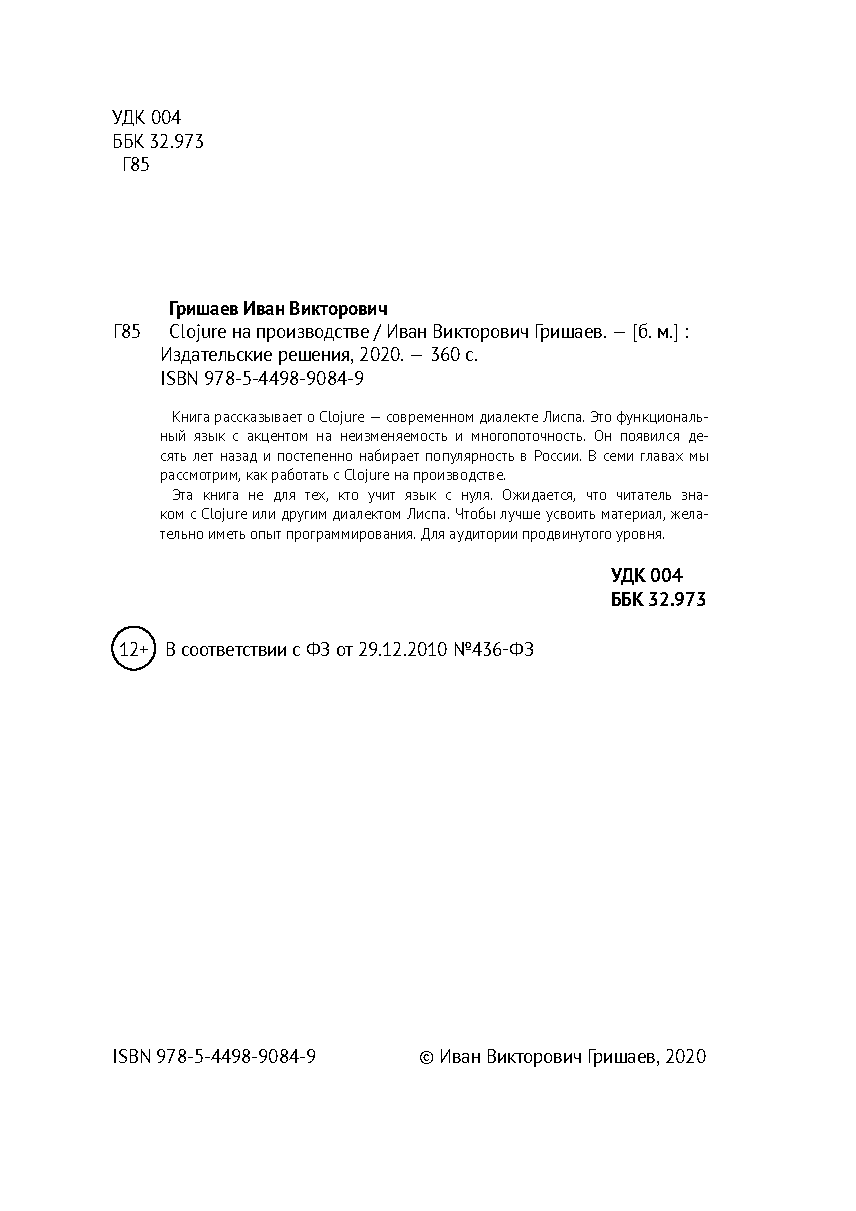
\includepdf[pages={1}]{media/ridero_opening.pdf}
\else
\thispagestyle{empty}

\small

Книга рассказывает о Clojure, современном диалекте Лиспа. Это функциональный
язык с акцентом на неизменяемость и многопоточность. Clojure появился десять лет
назад и плавно набирает популярность в России. В семи главах мы рассмотрим
проблемы, которые ждут вас на производстве.

Эта книга не для тех, кто учит язык с нуля. Ожидается, что читатель знаком с
Clojure или другим диалектом Лиспа. Чтобы лучше усвоить материал, желательно
иметь практический опыт программирования. Для аудитории продвинутого уровня.

\fi

%%
%% ToC https://tex.stackexchange.com/questions/41555/
%%
\let\Contentsline\contentsline
\renewcommand\contentsline[3]{\thispagestyle{empty}\Contentsline{#1}{#2}{#3}}
\cleardoublepage
\tableofcontents

\clearpage
\chapter*{Об этой книге}

У вас в руках книга о языке программирования Clojure. Это современный диалект
Лиспа, который работает на платформе JVM. От устаревших диалектов Clojure
отличается тем, что делает ставку на функциональный подход и неизменяемость
данных. Язык устроен так, чтобы решать сложные задачи максимально простым
способом.

Эта книга~--- не перевод. Она изначально написана на русском языке. Вы не
найдете тяжелых предложений, в которых отчетливо слышна английская речь. Вам не
придется читать <<маркер>> вместо <<токен>> и другую нелепицу. Все термины написаны
в том виде, чтобы быть понятными программисту.

В этой книге нет вводной части, где написано, что скачать и установить. Также мы
не рассматриваем базовые вещи вроде чисел и строк. На тему введения уже написаны
другие книги и посты в блогах. Автор считает, было бы нечестно предложить
читателю материал, который наполовину пересекается со сказанным ранее. Эта книга
от начала и до конца~--- то, о чем еще никто не писал.

Другое ее достоинство~--- упор на практику. Примеры кода взяты из реальных
Clojure-проектов. Все техники и приемы, упомянутые в книге, автор опробовал
лично. В описании проблем мы отталкиваемся от того, с чем вы столкнетесь на
производстве. Мы покажем, где теория расходится с практикой и что предпочесть в
таком случае.

Коротко о том, что вас ждет. Начнем с веб-разработки~--- вспомним протокол HTTP
и как с ним работать в Clojure. Затем рассмотрим Clojure.spec~--- библиотеку для
проверки данных. Третья глава рассказывает про исключения. Четвертая~--- про
изменяемые данные. Далее переходим к вопросам конфигурации. В шестой главе
знакомимся с компонентами и системами. В последней учимся писать тесты.

Даже если книга попала к вам случайно, и вы не любите Лисп, не спешите ее
откладывать. Clojure это другой мир и новые правила, а книга~--- шанс туда
попасть. Может быть, Clojure изменит ваше мнение о программировании. Обнаружит
вопросы там, где, казалось бы, все давно решено.

Автор будет признателен за указанные опечатки и неточности. Присылайте их по
адресу \spverb|ivan@grishaev.me|. Возможно, в промежутках между тиражами
получится обновить макет, и следующий читатель не увидит ошибки, о который вы
сообщили. И конечно, автор учтет все замечания при переводе на английский язык.

Пожелаем читателю терпения, чтобы прочесть книгу до конца.

\section*{Благодарности}

Спасибо стартапу Flyerbee, который стал моей первой работой на Clojure. Свои
скромные теоретические знания я обкатывал именно там.

Я счастлив работать в компании Exoscale в окружении талантливых мужчин и
женщин. О многих вещах, не только технических, я узнал благодаря им.

Спасибо Петру Маслову за крупную партию найденных опечаток. Досбол Жантолин внес
важное замечание к последней главе. Молодцы все, кто указывал на ошибки в
комментариях в блоге.

Благодарю коллектив издательства Геликон-Плюс за то, что взяли рукопись в
работу. Их усилиями вы читаете эту книгу сейчас.


\blank\chapter{Введение в~веб-разработку}

\begin{teaser}
В первой главе мы рассмотрим, как писать веб-приложения на Clojure. Поговорим о
том, как передают данные по протоколу HTTP. Какие абстракции строят поверх
протокола и что предлагает Clojure. Чем хорош функциональный подход и почему
разработка с~ним быстрее и~удобнее.
\end{teaser}

Каждый год компания Cognitect опрашивает\footnote{blog.cognitect.com/blog/2017/1/31/clojure-2018-results}
разработчиков на Clojure. Среди прочего в анкете вопрос о том, в какой области вы работаете? В~2010 году под
веб писали 50\% опрошенных, то есть каждый второй. К~2018 году
эта цифра выросла до 80\%. Это уже четыре человека из пяти. Похожую динамику показывают
опросы StackOverflow\footnote{insights.stackoverflow.com/survey/2018}.
Согласно им, все больше разработчиков переходит в веб из смежных областей.

Если вы найдете работу на Clojure, скорее всего это будет веб-приложение. Мы
специально не говорим <<сайт>>, чтобы подчеркнуть: термин уходит в
прошлое. Сегодня веб-приложение это не только HTML с картинками. В широком плане
это сложный обмен данными по протоколу HTTP.

Протокол разработан для передачи разметки, но удивительным образом подошел для
данных. Для этого даже не пришлось менять стандарт. Причина кроется в его
изящном дизайне, простоте и гибкости. Прежде чем перейти к Clojure, освежим в
памяти устройство протокола. Из каких частей он состоит и по каким правилам с
ним работает сервер. Это важно, потому что языки и фреймворки меняются, а
протокол нет.

\section{Основы HTTP}

HTTP это протокол, который работает поверх TCP/IP. В широком смысле протоколы~---
это соглашения о том, как читать и писать данные. Обычно они записаны в официальных
документах. Для HTTP такой документ называется RFC~2616\footnote{https://tools.ietf.org/html/rfc2616}.
Разработчики браузеров сверяются с~ним, чтобы технология работала
на разных языках и платформах.

HTTP удобен тем, что это текст. Разработчику не нужно декодировать байты, чтобы
понять, что происходит. Протокол передает и бинарные данные, но главные части
все же выражены текстом. В HTTP различают запрос и ответ. Оба состоят из трех
частей: \emph{первая строка}, \emph{заголовки} и \emph{тело}.

\emph{Первая (стартовая)} строка несет самую важную информацию. Ее формат
различается для запроса и ответа. Для запроса это метод, путь и версия, для
ответа~--- статус, сообщение и версия.

\emph{Заголовки} это пары ключ-значение. В современных фреймворках их
описывают словарем. Заголовки содержат дополнительные сведения о запросе или
ответе. Например, заголовок \spverb|Content-Type| сообщает, как трактовать тело
запроса. Был ли это XML- или JSON-документ? Программа проверяет заголовок
и~читает тело должным образом.

После заголовков следует \emph{тело}. Им может быть что угодно~--- текст, данные
в виде <<поле=значение>>, JSON-документ, картинка, фильм, электронное
письмо. Стандарт допускает смешанный тип, \spverb|multipart-encoding|. Тело
такого запроса разбито на ячейки, в каждом из которых свое содержимое. Например,
текст, картинка, снова текст, двоичный файл.

Рассмотрим примеры HTTP-трафика. Именно в таком виде он передается
по сети. Это запрос к главной странице Google, поисковой терм~--- \spverb|clojure|:

\begin{verbatim}
GET /search?q=clojure HTTP/1.1
Host: google.com
Accept-Language: en-us
Accept-Encoding: gzip, deflate
User-Agent: Mozilla/4.0 (compatible; MSIE 6.0; Windows NT 5.1)
(blank line)
\end{verbatim}

\noindent
А это POST-запрос с JSON-документом в теле:

\begin{verbatim}
POST /api/users/ HTTP/1.1
Host: example.com
Content-Type: application/json
User-Agent: Mozilla/4.0 (compatible; MSIE 6.0; Windows NT 5.1)

{
  "username": "John",
  "city": "NY"
}
\end{verbatim}

\noindent
Ответ на этот запрос:

\begin{verbatim}
HTTP/1.1 200 OK
Date: Tue, 19 Mar 2019 15:57:11 GMT
Server: Nginx
Connection: close
Content-Type: application/json

{
  "code": "CREATED",
  "message": "A user has been created successfully"
}
\end{verbatim}

Видно, как изящно устроен протокол. Данные в нем расположены по убыванию важности.
Прочитав только первую строку, клиент и сервер готовы принять решение о~том,
что делать дальше.

Рассмотрим сценарий: в запросе указаны метод и путь \spverb|GET /about|, но
такой страницы не существует. Сервер проверит это заранее, например, сверив путь
с конфигурацией маршрутов. Когда маршрута нет, вернется ответ со статусом
404. Не придется читать тело запроса, что ускорит работу сервера. Получив ответ,
клиент прочитает статус 404 из первой строки, что означает ошибку. Логика
клиента может быть такова, что для негативного статуса он не читает тело.

Чтение и разбор содержимого это дорогая операция. Современные фреймворки
исключают случаи, когда чтение происходит зря. Например, по заголовку
\spverb|Content-Type| мы определяем, стоит ли читать тело. Наше приложение
работает только с JSON, поэтому для значения \spverb|text/xml| вернем
ошибку. Аналогично с заголовком \spverb|Content-Length|, где содержится длина
тела в байтах. Если значение больше заданного лимита, сервер отклонит запрос еще
до чтения.

Центральные параметры запроса это \emph{метод} и \emph{путь}. Путь указывает на
определенный ресурс на сервере. Иногда сервер трактует путь как файл
относительно заданной папки. Например, \spverb|/images/map.jpg| означает вернуть
такой файл из \spverb|/var/www/static|. Но чаще всего путь обрабатывают по
внутренним правилам. Ответом может быть не только файл, но и js-скрипт,
HTML-разметка или JSON-документ.

\emph{Метод запроса} означает действие, которые мы намерены выполнить над
ресурсом. Основные методы это \spverb|GET|, \spverb|POST|, \spverb|PUT| и
\spverb|DELETE|. Их семантика в том же порядке~--- прочитать, создать, обновить,
удалить ресурс. Так, запрос \spverb|POST /users/| означает создать пользователя,
а \spverb|GET /users/|~--- получить их список.

Главный параметр ответа это \emph{статус}~--- целое положительное число. Статусы
группируют по старшему разряду. Значения с 200 до 299 (или \spverb|2хх|) считают
положительными. Они означают, что сервер обработал запрос без ошибки.

Значения из группы \spverb|3хх| связаны с перенаправлением на другую страницу.
В заголовке \spverb|Location| приходит путь, на который нужно послать
новый запрос. Браузеры и HTTP-клиенты достаточно умны, чтобы сделать это
автоматически. Например, при запросе страницы \spverb|http://yandex.ru| вы
получите пустой документ с заголовком \spverb|Location: https://yandex.ru|.
Сервер обязывает нас перейти на безопасное соединение. Но мы даже не заметим
этого: браузер сам сменит адрес.

Статусы из группы \spverb|4хх| означают ошибку на стороне клиента. Чаще всего это 404~---
страница не найдена. На ошибочные данные сервер отвечает 400~--- \spverb|Bad request|.
Когда нет прав доступа, клиент получит код 403.

Статусы из группы \spverb|5хх| говорят об ошибке сервера или его
недоступности. Это деление на ноль, отказ базы данных, недостаток места
на диске.

Принято считать, что ответ со статусом вне диапазона \spverb|2хх| означает
ошибку. Многие HTTP-клиенты бросают исключение на ответ с негативным статусом.
Строго говоря, это верно только на высоком, абстрактном уровне. С точки
зрения протокола ответ \spverb|404 Not Found| такой же правильный, как и \spverb|200 OK|.

Когда действий с ресурсом много, используют другие, более редкие
методы. Например, \spverb|HEAD|~--- получить краткие сведения о сущности. Сервис
Amazon S3 в ответ на HEAD-запрос вернет только статус и заголовки. В них указаны
тип файла и его размер, контрольная сумма, дата последнего изменения. В данном
случае \spverb|HEAD|-запрос предпочтительней GET. Метаданные хранят в особом
хранилище отдельно от файла. Доступ к нему обычно быстрее, чем к файлу на диске.

Подход <<метод-ресурс>> со временем вырос в то, что сегодня называется
\spverb|REST|\footnote{restapitutorial.com}. Сторонники
\spverb|REST| выделяют сущности и \spverb|CRUD|-операции над ними (\textbf{C}reate,
\textbf{R}ead, \textbf{U}pdate, \textbf{D}elete). Считается хорошим подход,
когда сущность задают через путь, например \spverb|/users/1|, а операцию~---
методом. Если это создание или изменение, данные читают из тела, где обычно записан
JSON-документ. Мы не будем задерживаться на \spverb|REST|, потому что это всего лишь
свод рекомендаций, не идеальный и не единственный.

Отметим, что протокол не заставляет следовать этим правилам. Разработчик вправе
работать с HTTP так, как это удобно в данном проекте. Например, принимать только
POST-запросы с данными в теле. Или только GET с параметрами строки. Верную
стратегию определяют инструменты, бизнес и потребители сервиса.

\section{Возвращаясь к Clojure}

Современные фреймворки строят абстракции над HTTP. Разработчик не читает запрос
по байтам вручную. Эту задачу берут на себя библиотеки. Взамен разработчик
получает набор классов, чтобы с их помощью выразить логику приложения. Типичный
веб-проект на Python или Java это комбинация нескольких классов. Как правило,
это \spverb|Application|~--- главная сущность проекта. Класс \spverb|Router|
определяет, на какой обработчик переключить входящий запрос~--- \spverb|Request|.
Обработчик~--- это класс \spverb|Handler| с методами \spverb|.onGet|,
\spverb|.onPost| и тд. Ожидается, что он вернет экземпляр класса \spverb|Response|.

По такому принципу устроены промышленные веб-фреймворки: Django, Rails,
Symfony. Названия классов и их комбинация отличаются, но смысл остается
прежним. Это приложение, роутер, обработчик, запрос и ответ. Проблема в том, что
классы одного фреммворка не работаю с другим и наоборот.

Рассмотрим язык Python и фреймворки Django и Flask. Оба следуют той же
структуре. Так, запрос в Django описан в классе \spverb|django.http.HttpRequest|,
а во Flask~--- \spverb|flask.Request|. Даже беглого взгляда достаточно,
чтобы увидеть, насколько они отличаются. У классов разные методы и поля.
То, что есть в первом классе, отсутствует во втором. Использовать \spverb|flask.Request|
в проекте на Django невозможно.

Со временем проект увязает в архитектуре фреймворка. Переезд на другое решение
становится все менее возможным. Хорошие практики предлагают делить проект на
слои. Слой транспорта отвечает за ввод и вывод данных по протоколу HTTP. Слой
логики исполняет внутренний код, ничего не зная о HTTP. С таким подходом логика
не зависит от транспорта, и последний можно сменить в любой момент. Но на
практике это работает не всегда. По разным причинам слои перемешиваются. Мы
обещаем, что в следующий раз не допустим этого, и все повторяется сначала.

В Clojure другой подход.

Разработчик Джеймс Ривз (James Reeves) известен своим вкладом в экосистему
Clojure. Он разработал 60 библиотек\footnote{github.com/weavejester} для разных
задач. Нет такого проекта на Clojure, который бы не использовал его
наработки. Заслуга Джеймса в том, что он вывел стандарт веб-разработки для
Clojure на заре языка. Вместо того, чтобы писать фремворк под сиюминутные нужды,
он придумал, как сделать удобно всем.

Джеймс предложил несколько простых идей. Первая~--- если приложение принимает
запрос и возвращает ответ, то резонно \emph{выразить его функцией}. Действительно,
приложения бывают сколь угодно сложным. Они полагаются на сторонние сервисы,
машинное обучение, учитывают сотню фактов о пользователе. Но они принимают
запрос и возвращают ответ, поэтому на абстрактном уровне это \emph{функция}.

Скептики заметят, что мысль не нова. В том же Django обработчик бывает
не классом, а функцией. Разница в том, что отдельный обработчик~--- это
еще не приложение. Ему не хватает роутера, middleware и других абстракций.
Поэтому в Django или Flask выразить обработчик функцией~--- всего лишь
приятная возможность, сахар.

В Clojure приложение остается функцией на всех уровнях. Маршрутизатор~--- это
функция, которая принимает запрос, определяет обработчик и передает ему
управление. Middleware это тоже функция, которая дополняет приложение новой
логикой. Каждую тяжелую абстракцию (классы \spverb|Application|,
\spverb|Router|, \spverb|Handler|) в мире Clojure заменяют функцией. Это удобно,
потому что в отличии от классов функции стыкуются между собой.

Вторая идея Джеймса в том, чтобы зафиксировать структуру запроса и
ответа. Должны быть документы (не код, а \emph{именно документы}), где описаны
поля структур и их семантика. Это напоминает протокол HTTP. Спецификация
упрощает код и делает его переносимым. Два веб-проекта на Clojure принимают и
отдают одинаковые структуры данных. Разработчик очередного фреймворка учитывает
спецификацию. Если фреймворк следует стандарту, проще привлечь сообщество.

\subsection{Ring}

Идеи нашли применение в проекте Ring\footnote{github.com/ring-clojure/ring}.
Сегодня это стандарт веб-разработки на Clojure. Репозиторий содержит спецификацию
запроса и ответа и базовый код для работы с ними. Прилагаются основные
middleware, запуск Jetty-сервера и документация. Удивительно, как мало кода
понадобилось проекту, чтобы попасть на компьютер каждому Clojure-разработчику.

Со временем появился термин <<Ring-совместимость>>. Ему следуют все
фреймворки на Clojure. Типичное Ring-приложение запускается на многих платформах:
Jetty, Netty и других без изменений в коде.

Библиотека Ring разбита на отдельные части, чтобы можно было установить только
необходимое. Перечислим компоненты, которые понадобятся по ходу главы:


\begin{itemize}
\item
  \spverb|ring-core|~--- базовая функциональность: параметры, разбор тела, куки, сессии;

\item
  \spverb|ring-jetty-adapter|~--- запуск сервера из функции-приложения.

\end{itemize}

Первое приложение вы напишете даже без библиотеки. Вот оно:

\begin{verbatim}
(defn app [request]
  (let [{:keys [uri request-method]} request]
    {:status 200
     :headers {"Content-Type" "text/plain"}
     :body (format "You requested %s %s"
                   (name request-method) uri)}))
\end{verbatim}

Приложение извлекает путь и метод из запроса и формирует ответ. Его статус
положительный~--- 200. Мы выставили заголовок с типом документа <<простой
текст>>. Поле \spverb|:body| содержит строку, которую строим функцией \spverb|format|.

Поскольку \spverb|app| это функция, вызовем ее с различными запросами:

\begin{verbatim}
(app {:request-method :get :uri "/index.html"})
{:status 200,
 :headers {"Content-Type" "text/plain"},
 :body "You requested get /index.html"}

(app {:request-method :post :uri "/users"})
{:status 200,
 :headers {"Content-Type" "text/plain"},
 :body "You requested post /users"}
\end{verbatim}

Работает. Но пока что это структуры данных, и не ясно, что будет в
браузере. Запустим приложение в виде сервера.

Сервер это отдельная сущность. Он связывает структуры данных с сетевым
вводом-выводом. Сервер принимает приложение с параметрами и запускает в фоне
сложный процесс. Он слушает указанный порт и читает байты. Из бинарных
данных получается словарь запроса. В отдельном треде сервер вызывает проложение с
этим запросом. Результатом будет словарь ответа. Сервер переводит ответ в
байтовый поток и пишет в удаленный порт клиента. Этот цикл повторяется для
каждого запроса.

Добавим в проект зависимости:

\begin{verbatim}
[ring/ring-core "1.7.1"]
[ring/ring-jetty-adapter "1.7.1"]
\end{verbatim}

Запустим сервер:

\begin{verbatim}
(require '[ring.adapter.jetty :refer [run-jetty]])
(run-jetty app {:port 8080 :join? true})
\end{verbatim}

Происходит следующее. Мы импортировали в текущее пространство функцию
\spverb|run-jetty|. Она принимает два параметра~--- приложение и словарь
опций. Ключ \spverb|join?| определяет, будет ли заблокирован текущий тред до
конца работы сервера. Если передать \spverb|false|, сервер запустится в
фоне. Чтобы остановить его, нужно запомнить результат \spverb|run-jetty| в
переменную и вызвать у него метод \spverb|.stop|:

\begin{verbatim}
(def server
  (run-jetty app {:port 8080 :join? false}))

;; after a while
(.stop server)
\end{verbatim}

Если флаг был \spverb|true|, как в первом случае, главный поток повиснет до
конца работы сервера. Придется либо завершить программу, либо нажать
\spverb|Ctrl-C|. Пока сервер работает, откройте браузер по адресу \spverb|127.0.0.1:8080|.
Вы увидите строку из примера выше. Впишите другой путь, например \spverb|/hello| или
\spverb|/path/to/file.txt|. Ответ сервера изменится.

\section{Запросы и ответы}

Мы написали приложение, которое на все запросы печатает метод и путь. Кроме этих
полей, запрос содержит порт и адрес сервера, строку параметров, тип протокола,
заголовки и тело. Все вместе это неизменяемый словарь с ключами типа
\spverb|keyword| (кейворды или ключевые слова, в других языках~--- теги). Полное
описание запроса и ответа лежит в репозитории
на Гитхабе\footnote{github.com/ring-clojure/ring/blob/master/SPEC}.

Обратим внимание на поля \spverb|:headers| и \spverb|:body|.

Заголовки это неизменяемый словарь, но его ключи не кейворды, а строки. Такой
словарь не работает привычным с destructuring assignment. Ниже переменная \spverb|host|
окажется \spverb|nil|:

\begin{verbatim}
(defn some-handler
  [request]
  (let [{:keys [headers]} request
        {:keys [host]} headers]
    ...))
\end{verbatim}

Чтобы извлечь заголовки правильно, используйте \spverb|:strs|:

\begin{verbatim}
(defn some-handler
  [{:keys [headers]}]
  (let [{:strs [host user-agent]} headers]
    ...))
\end{verbatim}

\noindent
или обычный \spverb|get| со строкой:

\begin{verbatim}
(get headers "host") ;; "127.0.0.1"
\end{verbatim}

Имя заголовка всегда в нижнем регистре. С точки зрения HTTP варианты
\spverb|Content-Type| и \spverb|content-type| одинаковы. \spverb|Ring| приводит заголовки к
нижнему регистру, чтобы избежать недоразумений.

Значения заголовков тоже строки. Даже если стандарт задает типы некоторым
заголовкам, \spverb|Ring| не выводит их. Например,  \spverb|Content-Length|
передает длину тела в байтах. Современные фреймворки
приводят его к числу и помещают в отдельное поле. По умолчанию Ring не делает
ничего подобного, но это легко исправить.

С заголовками связана одна проблема. В Clojure ключи словаря почти всегда
кейворды. Легко забыть, что у заголовков они строки. Так появляется ошибка,
когда вместо правильного значения приходит \spverb|nil|:

\begin{verbatim}
(get headers :host) ;; nil
\end{verbatim}

Можно обработать заголовки, заменив тип ключей. Для одного случая это
нормально. Но если этим занят каждый обработчик, получается лишняя
работа. Приложение меняют так, чтобы в функцию приходили уже исправленные
заголовки. Эта техника называется Middleware, и мы рассмотрим ее ниже.

Поле запроса \spverb|:body| опционально. Согласно HTTP тела может и не быть. При
попытке считать \spverb|:body| проверяйте его на \spverb|nil|. Обратите внимание
на тип тела. Это не строка, а входящий поток~---
\spverb|java.io.InputStream|. Поток~--- это источник данных, который можно
прочесть только раз. По умолчанию \spverb|Ring| не читает поток. Делать это или нет
остается на ваше усмотрение.

Чтение и разбор тела это сложная операция. По заголовкам
определяют тип документа, его длину и читают нужное число байт. Из них
восстанавливают данные (JSON, XML). Результат каждого шага проверяют по разным
критериям. Когда из \spverb|Content-Length| получают число, перехватывают
исключение разбора строки. Результат \spverb|-42| неверный, потому что число байт не
может быть отрицательным. Технически возможно послать серверу JSON-документ, но
указать тип \spverb|text/xml|. Сервер должен быть готов к подобным сценариям.

Легче всего считать тело в строку функцией \spverb|slurp|:

\begin{verbatim}
(defn handler [request]
  (when-let [content (some-> request :body slurp)]
    (process-content content))
  {:status 200})
\end{verbatim}

Но в современном вебе все меньше работают с текстом: на его место приходят данные в виде
JSON. Позже мы рассмотрим, как подружить Ring с этим форматом.

\subsection{Структура ответа}

Ответ \spverb|Ring| устроен проще. Это словарь с тремя полями:
\spverb|:status|, \spverb|:headers| и \spverb|:body|.

\begin{itemize}

\item
  \spverb|:status|~--- целое положительное число, признак успеха или неудачи. Мы
  рассмотрели семантику статуса в начале главы.

\item
  \spverb|:headers|~--- заголовки ответа. В отличии от запроса, ключи и
  значения не обязательно строки. Вариант ниже работает:

\begin{verbatim}
{:status 302
 :headers {:content-length 0
           :location "/new/page.html"}}
\end{verbatim}

\item
  \spverb|:body|~--- тело ответа. Как и в запросе, его может не быть. Обычно тело
  это строка, но может быть и файлом, ресурсом или потоком.

\end{itemize}

\section{Маршруты}

Мы запустили приложение и проверили его в браузере. На любой запрос оно выдает
текст с небольшими отличиями. Это слабый подход: невозможно поддерживать
приложение, в котором все запросы сходятся в одну точку. На практике пишут
отдельные обработчики для каждой задачи. Затем распределяют по ним входящие
запросы согласно правилам. Это называется маршрутизация или роутинг.

В мире Clojure и Ring нет класса роутера. Это функция, которая принимает
обработчики (хендлеры) и возвращает новую функцию-приложение. Она принимает
запрос и по методу и пути подбирает нужный обработчик. Затем вызывает его с
запросом и возвращает ответ.

Рассмотрим тривиальный случай. Вообразим, что адресу \spverb|/| мы бы хотели видеть
название сайта, а по \spverb|/hello|~--- приветствие. Все другие адреса вернут
\spverb|404 Page not found|. Напишем обработчики:

\begin{verbatim}
(defn page-index [request]
  {:status 200
   :headers {:content-type "text/plain"}
   :body "Learning Web for Clojure"})

(defn page-hello [request]
  {:status 200
   :headers {:content-type "text/plain"}
   :body "Hi there and keep trying!"})

(defn page-404 [request]
  {:status 404
   :headers {:content-type "text/plain"}
   :body "No such a page."})
\end{verbatim}

Каждый обработчик можно запустить как сервер и проверить в браузере. Осталось
связать их в единое целое.

\subsection{Наивный подход}

Сделаем самое простое, что приходит в голову. Напишем обработчик, который
вручную определяет маршрут. Для этого проверим путь оператором \spverb|case|:

\begin{verbatim}
(defn app [request]
  (let [{:keys [uri]} request]
    (case uri
      "/"      (page-index request)
      "/hello" (page-hello request)
      (page-404 request))))
\end{verbatim}

Ответ такой функции зависит от поля запроса \spverb|:uri|. Запустите приложение
в браузере и проверьте разные адреса. Это наивный перебор, но он работает.

Недостатки функции очевидны. Мы не учитываем метод запроса. \spverb|GET /users| и
\spverb|POST /users| отличаются по смыслу. Мы сравниваем пути в лоб без
учета параметров. В правильном роутинге запросы \spverb|GET /users/1|
и \spverb|GET /users/99| приходят в один обработчик, но с разным параметром \spverb|id|.
В целом код зашумлен. Хотелось бы иметь маршруты в виде правил без перебора.

Эти и другие проблемы решены в библиотеках. Мы рассмотрим две
из них: \spverb|Compojure| и \spverb|Bidi|. Обе решают задачу роутинга по-своему, их
подходы ортогональны.

\subsection{Compojure}

Библиотека \spverb|Compojure|\footnote{github.com/weavejester/compojure}
предлагает макросы для описания маршрутов. Макросы похожи на таблицу правил.
Добавим зависимость в проект:

\begin{verbatim}
[compojure "1.6.1"]
\end{verbatim}

\noindent
Вот как выглядит приложение на Compojure:

\begin{verbatim}
(require '[compojure.core :refer [GET defroutes]])

(defroutes app
  (GET "/"      request (page-index request))
  (GET "/hello" request (page-hello request))
  page-404)
\end{verbatim}

\noindent

Эта запись чище и короче той, что мы написали вначале.

Разберемся, что получилось на выходе. Переменная \spverb|app|~--- функция, которая
принимает запрос. Мы объявили ее не через \spverb|def| или \spverb|defn|,
а особым макросом. Мы поговорим о макросах в отдельной главе. Пока что
скажем, что \spverb|defroutes| делает две вещи: строит функцию-роутер и связывает ее с
переменной \spverb|app|. Это уловка, чтобы писать меньше кода.

Макрос принимает правила. Правило это форма <<метод, путь, запрос,
выражение>>. Первые два правила заданы макросом \spverb|GET|. Они читаются так: если
метод равен \spverb|GET| и путь \spverb|"/"|, то для запроса \spverb|request|
вернуть \spverb|(page-index request)|.

Правило компилируется в функцию, которая принимает запрос. Функция проверяет,
что метод и путь запроса совпадают с заданными. Если да, функция вычислит
выражение и вернет его результат, в нашем случае \spverb|(page-index request)|.

Если совпадения не было, функция вернет \spverb|nil|. Это
значит, надо взять следующее правило и так далее. Макрос \spverb|defroutes|
работает по этой схеме. Он оборачивает правила в особый цикл. На каждом
шаге макрос берет очередное правило, применяет к нему запрос и оценивает
результат. Первое значение, отличное от \spverb|nil|, станет ответом к текущему запросу.

Что будет, если не подошло ни одно правило? Это вполне возможно. Если
приложение вернуло \spverb|nil|, это вызовет ошибку сервера. Чтобы избежать \spverb|nil|,
к правилам добавляют еще одно, которое сработает всегда. В нашем случае это функция \spverb|page-404|.
Ее результат не зависит от запроса. Этим мы гарантируем, что даже если запрос не подошел
первым двум правилам, последнее сработает обязательно.

Так работает роутинг на \spverb|Compojure|. Приложение разбивают на обработчики.
Их пишут в отдельных модулях, затем с помощью макросов \spverb|GET|, \spverb|POST|
и других оборачивают в правила. Правило возвращает функцию, которая
проверяет, что метод и путь подходят. Если да, в результате получим вызов
обработчика с запросом.

\subsection{Продвинутые возможности}

Выше мы обозначили проблему: правила \spverb|GET /users/1| и \spverb|GET /users/99|
это один обработчик с параметром. Его записывают так:

\begin{verbatim}
(GET "/users/:id" [id :as request] (page-user request))
\end{verbatim}

Обратите внимание на двоеточие перед \spverb|id| и квадратные скобки в середине.
Часть пути с двоеточием означает параметр. \spverb|Compojure| поместит его в словарь
\spverb|params|. Обработчик \spverb|page-user| обратится к нему следующим образом:

\begin{verbatim}
(defn page-user [request]
  (when-let [user-id (-> request :params :id)]
    (let [user (get-user-by-id user-id)
          {:keys [fname lname]} user]
      {:status 200
       :body (format "User %s is %s %s"
                     user-id fname lname)})))
\end{verbatim}

В данном случае мы решили, что функция \spverb|get-user-by-id| вернет словарь
пользователя по номеру. Из словаря извлекаем имя и фамилию, формируем
строку и возвращаем ответ.

\spverb|Compojure| решает проблему вложенных путей. Предположим, приложение показывает и
редактирует товары. По адресу \spverb|/content/order/1/view| открывается карточка
товара. Страница \spverb|/content/order/1/edit| показывает форму редактирования этого товара.
Чтобы сохранить товар, нужно отправить форму по тому же пути, но методом \spverb|POST|.

Очевидно, правила пересекаются. Чтобы избежать повторов, используем макрос \spverb|context|:

\begin{verbatim}
(context "/content/order/:id" [order-id]
  (GET  "/view" request (order-view request))
  (context "/edit" []
    (GET  "/" request (order-form request))
    (POST "/" request (order-save request))))
\end{verbatim}

Каждое правило под макросом \spverb|context| наследует параметры запроса. Это значит,
обработчики \spverb|order-view|, \spverb|order-form| и \spverb|order-save| получат
параметр \spverb|:order-id|.

До сих пор качестве ответа в правилах мы писали что-то вроде
\spverb|(some-handler request)|. Бывает, что ответ заранее известен,
поэтому нет смысла помещать его в отдельную функцию. Рассмотрим это на примере
\spverb|healthcheck|-обработчика.

Современные приложения запускают в контейнерах и облачных сервисах.  Чтобы
узнать, работает приложение или нет, специальная служба периодически опрашивает
его. Привычный способ сделать это~--- послать приложению \spverb|GET|-запрос по адресу
\spverb|/health| и проверить статус. Тело и заголовки ответа не играют роли.

Чтобы не создавать лишний обработчик \spverb|(page-health request)|, поместим ответ в
тело:

\begin{verbatim}
(ANY "/health" _ {:status 200 :body "ok"})
\end{verbatim}

Можно сделать еще проще. В \spverb|Compojure| предусмотрен случай, когда
выражение это строка. Для \spverb|Compojure| она становится телом положительного
ответа:

\begin{verbatim}
(ANY "/health" _ "ok")
\end{verbatim}

\subsection{Роутинг с Bidi}

Библиотека Bidi\footnote{github.com/juxt/bidi} решает проблему роутинга по-другому.
\spverb|Compojure| предлагает макросы, чтобы задать правила и сделать по ним перебор. \spverb|Bidi|
опирается на данные~--- списки и словари. Этот сценарий состоит из нескольких шагов.

На \emph{первом этапе} объявляют дерево маршрутов. Это дерево~--- комбинация
векторов и словарей по определенным правилам. В листьях дерева помещают теги~---
уникальные метки. Особая функция принимает это дерево и запрос. Функция пытается понять,
на какую ветку дерева он ложится. Если ветку нашли, результатом будет ее тег и, возможно,
параметры пути. Например, \spverb|{:route :show-user, :route-params: {:id 1}}|.

На \emph{втором этапе} пишут middleware~--- промежуточный обработчик запроса.
Он принимает запрос, добавляет в него тег и передает дальше по цепочке.

На \emph{третьем этапе} пишут обработчик запроса. Но это не функция, а мультиметод.
Его функция-диспатчер возвращает тег. Метод с тегом \spverb|:default| возвращает
ответ \spverb|404|, \spverb|:show-user|~--- страницу пользователя и так далее.

На первый взгляд схема кажется сложной. Но однажды настроив, ее легко
расширять. Чтобы сервер подхватил новый путь, в дерево добавляют ветку и
расширяют мультиметод.

Перепишем на \spverb|Bidi| все то, что сделали на \spverb|Compojure|. Добавьте в проект
зависимость:

\begin{verbatim}
[bidi "2.1.5"]                  ;; project.clj
(:require [bidi.bidi :as bidi]) ;; namespace
\end{verbatim}

Начнем с дерева маршрутов. Вариант с \spverb|page-index|, \spverb|page-hello|
и \spverb|page-404| выглядит так:

\begin{verbatim}
(def routes
  ["/" {""      :page-index
        "hello" :page-hello
        true    :not-found}])
\end{verbatim}

Проверим, как работает матчинг пути по этому дереву. Функция \spverb|match-route|
принимает маршруты, путь и возвращает словарь с тегом:

\begin{verbatim}
(bidi/match-route routes "/hello")
{:handler :page-hello}

(bidi/match-route routes "/test")
{:handler :not-found}
\end{verbatim}

Объединим тег со словарем запроса. Чтобы сделать это за один шаг, воспользуемся
функцией \spverb|match-route*|. Это альтернативная версия \spverb|match-route|, которая принимает
словарь-накопитель. Роль накопителя сыграет запрос.

\begin{verbatim}
(let [request {:request-method :get
               :uri "/test"}]
  (bidi/match-route* routes (:uri request) request))

{:request-method :get
 :uri "/test"
 :handler :not-found}
\end{verbatim}

Видим, что \spverb|match-route*| вернула запрос, но добавила в него поле
\spverb|:handler|. Перепишем этот код на middleware. Это функция, которая
принимает обработчик и возвращает его измененную версию. Получив запрос, новый
обработчик добавит к нему поле \spverb|handler| и передаст в исходный
обработчик.

\begin{verbatim}
(defn wrap-handler [handler]
  (fn [request]
    (let [{:keys [uri]} request
          request* (bidi/match-route* routes uri request)]
      (handler request*))))
\end{verbatim}

Мы еще не касались техники middleware, но вынуждены применить ее сейчас. Ниже мы
рассмотрим в деталях, как они работают и почему так важны.

Проверим \spverb|wrap-handler| на скорую руку. Для удобства обернем функцию
\spverb|identity|. Она возвращает переданный в нее аргумент:

\begin{verbatim}
((wrap-handler identity)
 {:request-method :get
  :uri "/hello?foo=42"})

{:request-method :get,
 :uri "/hello?foo=42",
 :handler :page-hello}
\end{verbatim}

Обработчик запроса будет мультиметодом. Его функция-диспатчер просто
\spverb|:handler|.

\begin{verbatim}
(defmulti multi-handler :handler)

(defmethod multi-handler :page-index
  [request]
  {:status 200
   :headers {:content-type "text/plain"}
   :body "Learning Web for Clojure"})

(defmethod multi-handler :not-found
  [request]
  {:status 404
   :headers {:content-type "text/plain"}
   :body "No such a page."})
\end{verbatim}

Обернем \spverb|multi-handler| в middleware. Это и будет финальное
приложение. Запустите веб-сервер и проверьте результат в браузере.

\begin{verbatim}
(def app (wrap-handler multi-handler))
\end{verbatim}

Это был простой роутинг на \spverb|Bidi|. Теперь рассмотрим сценарий с товарами,
их просмотром и изменением. Новое дерево выглядит так:

\begin{verbatim}
(def routes
  ["/" {["content/order/" :id]
        {"/view" {:get  :page-view}
         "/edit" {:get  :page-form
                  :post :page-save}}}])
\end{verbatim}

В этой версии листья уже не теги, а словари. Ключ каждого словаря~--- метод
HTTP-запроса, а значение~--- тег. Запрос \spverb|GET /content/order/1/edit|
разрешается в тег \spverb|:page-form|, а \spverb|POST| с таким же адресом~--- в \spverb|:page-save|.
На этапе \spverb|wrap-handler| запрос получит поле \spverb|:route-params|.
В нашем случая это словарь \spverb|{:id "1"}|.

Набросаем штрихи обработчиков. \spverb|Page-view| находит товар по номеру и
верстает HTML-страницу с ним. Если товара нет, вернем ответ 404 <<не найдено>>.

\begin{verbatim}
(defmethod multi-handler :page-view
  [request]
  (if-let [order (-> request :route-params :id get-order-by-id)]
    {:status 200
     :headers {:content-type "text/html"}
     :body (render-order-page {:order order})}
    response-404))
\end{verbatim}

Страница с формой \spverb|:page-form| отличается тем, что вместо
\spverb|render-order-page| мы бы вызвали \spverb|render-order-form|. Эта
функция верстает HTML-форму с кнопками. Обновление товара сложнее: нужно выбрать поля из
запроса и записать их а базу. Для краткости опустим валидацию:

\begin{verbatim}
(defmethod multi-handler :page-save
  [request]
  (let [{:keys [params route-params]} request
        {order-id :id} route-params
        fields (select-keys params [:title :description :price])]
    (jdbc/update! *db* :orders fields ["id = ?" order-id])
    {:status 302
     :headers {:Location (format "/content/order/%s/view" order-id)}}))
\end{verbatim}

Обратите внимание: на изменение данных мы отвечаем не HTML-страницей, а
\emph{редиректом} на нее. Если браузер получил страницу в результате
\spverb|POST|-запроса, то при попытке ее обновить браузер снова отправит
форму. Это чревато спонтанными изменениями на сервере. Вариант с редиректом решает
эту проблему. Браузер загрузит страницу через \spverb|GET|, и побочных эффектов
при обновлении не будет.

%% ------------

\subsection{Выбор между Compojure и Bidi}

Автору приходилось работать с роутингом обоих типов. По субъективным ощущениям,
с Compojure легче начать. У библиотеки достойная документация с
примерами. Compojure написал тот же разработчик, что и Ring. Проекты близки и
дополняют друг друга.

Дерево маршрутов Bidi сложно для понимания. Оно многословно и не
интуитивно. Легко допустить ошибку, перепутать вектор и словарь. С другой
стороны, логика на мультиметодах несет преимущества. Код становится линейным,
более организованным, приложение легче наращивать.

Если вы начинающий Clojure-разработчик или проект небольшой, выбирайте
Compojure. Когда проект сложный со множеством эндпоинтов, рассмотрите переезд на
Bidi.

\section{Middleware}

Выше мы упоминали про middleware и даже кинули пробный шар~--- написали
wrap-route. В этом разделе мы разберем все вопросы о middleware и лучших
практиках по работе с ними. Автор считает этому тему самой важной в главе.

В переводе с английского Middleware значит промежуточный слой, середина. В
программировании под middleware понимают код, который обрабатывает данные между
посредниками. Обработка данных это приведение типов, добавление новых полей,
проверка прав доступа.

Паттерн <<декоратор>> это частный случай middleware. Декоратор это функция А,
которая принимает функцию B и возвращает функцию C. Говорят, что A декорирует
B. Результат декорирования это C. В ходе исполнения функция C вызывает B, но с
изменениями. Например, корректирует входные или выходные данные B.

Приведем примеры простых декораторов. with-echo добавляет к функции побочные
эффекты: печатает аргументы и результат.

\begin{verbatim}
(defn with-echo
  [func]
  (fn [& args]
    (apply println "The args are" args)
    (let [result (apply func args)]
      (println "The result is" result)
      result)))
\end{verbatim}

\spverb|With-catch| оборачивает целевую функцию в форму \spverb|try/catch|. Если во время
работы выброшено исключение, результатом будет его объект.

\begin{verbatim}
(defn with-catch
  [func]
  (fn [& args]
    (try
      (apply func args)
      (catch Throwable e
        e))))
\end{verbatim}

Мы уже рассматривали структуру Ring-запроса. Возможно, читатель заметил, что в
нем нет полей, с которыми он работал в других языках. Например, классы
\spverb|django.http.HttpRequest| и \spverb|flask.Request| в Python содержат поля \spverb|.params| или
\spverb|.values|. Это словари, полученные из адресной строки или тела запроса.

Почему в стандарте Ring нет столь важных вещей? Потому что не каждое приложение
в них нуждается. Фреймворк предоставляет только базовую информацию о
запросе. Остальные данные могут быть получены из исходных.

Представим, что на каждый запрос Ring парсит строку параметров и тело. Это
удобно разработчику, но резко снижает производительность сервера. Нет гарантии,
что параметры строки пригодятся в запросе. Но сервер потратит время и память на
их обработку. Еще хуже с обработкой тела. Вспомним, что это дорогая
операция. Возможен сценарий, когда сервер прочитал огромный JSON-документ, но
внутри обработчика выяснилось, что у пользователя нет прав на запись. Эту
проверку следовало выполнить раньше!

Как мы помним, обработчик запроса в Ring это функция, которая принимает запрос и
возвращает ответ. Техника middleware как нельзя лучше подходит, чтобы добавить
промежуточную логику. Параметры запроса, сессии, куки, права доступа~--- все это
функция, которая возвращает функцию.

Вам не придется писать все middleware с нуля. Ring уже содержит основные из
них. Остается только применить их к приложению. Рассмотрим некоторые middleware
и принципы их работы.

\subsection{Параметры запроса}

Стандарт HTTP разрешает передавать данные в адресной строке. Это пары вида
\spverb|"name=John&city=NY"| после знака вопроса. Удобно, когда параметры доступны в виде
словаря. В нашем случае это была бы структура \spverb|{:name "John" :city "NY"}|.

Аналогично с параметрами из тела запроса. Их передают в теле по разным
причинам. В основном это ограничение на длину и проблемы безопасности. Длина
адресной строки ограничена 2048 байтами, в то время как на тело запроса
ограничений нет. Пароли и адреса почты небезопасно передавать в адресной строке,
потому что они остаются в логах и истории браузера.

Функция wrap-params из модуля ring.middleware.params меняет функцию-обработчик
следующим образом. Переданный в нее запрос дополняется тремя полями:

%% TODO list
- \spverb|:query-params|~--- словарь параметров адресной строки;
- \spverb|:form-params|~--- словарь данных из тела запроса;
- \spverb|:params|~--- их комбинированная версия.

Пусть \spverb|app|~--- ваше веб-приложение. Чтобы получить его обернутую версию,
достаточно вызвать wrap-params c app. Результат будет финальным приложением. На
жаргоне разработчиков это называется "врапнуть" (анг. wrap~--- обернуть).

\begin{verbatim}
(require '[ring.middleware.params
           :refer [wrap-params]])

(def final-app
  (wrap-params app))
\end{verbatim}

Чтобы не запутаться в именах, придерживайтесь правил. Не обернутое приложение
называйте \spverb|app-naked| или \spverb|app-raw| (голое, сырое), а финальное просто \spverb|app|.

Доработайте веб-приложение из примера выше так, чтобы оно учитывало параметры
строки. Например, чтобы имя того, кого приветствовать, можно было задать
параметром who: /hello?who=John.

Подсказка: добраться до параметра who можно так:

\begin{verbatim}
(defn page-hello
  [request]
  (let [who (get-in request [:params "who"])]
    ...))
\end{verbatim}

или так:

\begin{verbatim}
(defn page-hello
  [request]
  (let [who (-> request :params (get "who"))]
    ...))
\end{verbatim}

Обратите внимание, что ключи \spverb|:params| это строки. Это нормально, но Clojure
всячески поощряет нас, когда ключи словаря кейворды. Исправим это. В поставке
Ring есть особое middleware, которое приводит поле \spverb|:params| к удобному
виду. Это \spverb|wrap-keyword-params| из модуля \spverb|ring.middleware.keyword-params|:

\begin{verbatim}
(require '[ring.middleware.keyword-params
           :refer [wrap-keyword-params]])

(def app
  (wrap-keyword-params (wrap-params app-naked)))
\end{verbatim}

Мы подошли к новой проблеме: когда врапперов много, от них возникает
шум. Типичное приложение включает десять-пятнадцать middleware:

\begin{verbatim}
(def app
  (wrap-something-else
    (wrap-current-user
      (wrap-session
        (wrap-keyword-params
          (wrap-params app-naked))))))
\end{verbatim}

Это кашу невозможно поддерживать. Представьте, что требуется добавить еще один
враппер где-то в середине. Это каскадно сдвинет элементы ниже. Чтобы победить
сложность, сделаем структуру линейной. Применим стрелочный оператор:

\begin{verbatim}
(def app
  (-> app-naked
      wrap-params
      wrap-keyword-params
      wrap-session
      wrap-current-user
      wrap-something-else))
\end{verbatim}

Такая форма напоминает обычный список, поэтому ее легко поддерживать.

Запись в стрелочном виде имеет особенность. Не заглядывая в следующее
предложение, догадайтесь, в каком порядке будут выполнены middleware? Правильный
ответ: снизу вверх для запроса и сверху вниз для ответа. Это может показаться
странным, но становится очевидным при мысленном разборе.

Сперва запрос зайдет в \spverb|wrap-something-else|. Код внутри него вызовет
обработчик, который получен из \spverb|wrap-current-user|. Обработчик внутри него –
результат \spverb|wrap-session|, и так далее. Вершиной подъема станет
\spverb|app-naked|. Структура ответа начнет опускаться по стеку вниз. Сначала он
пройдет через \spverb|wrap-params| и \spverb|wrap-keyword-params|. Эти два middleware не
изменяют ответ и просто возвращают его. \spverb|Wrap-session| и \spverb|wrap-current-user|,
возможно, допишут в него новые заголовки. Последним сработает
\spverb|wrap-something-else|. Цикл запроса и ответа пройден.

Цепочку middleware следует рассматривать как восхождение в гору и спуск с
нее. Другой аналогией может быть пузырек, который всплывает и опускается (не
имеет отношения к сортировке пузырьком).

По тому же принципу устроены middleware в Django, промышленном
Python-фреймворке. Хоть в Django их роль играют не функции, а классы, их порядок
обхода такой же.

Порядок middleware порой критичен. Некоторые из них опираются на данные, которые
подготовили предыдущие middleware. Рассмотрим уже знакомые \spverb|wrap-params| и
\spverb|wrap-keyword-params|. Последний отыскивает в запросе поле params и меняет тип
ключей. Подразумевается, что params был подготовлен
\spverb|wrap-keyword-params|. Поэтому \spverb|wrap-keyword-params| ставят строго после
\spverb|wrap-params|.

Посмотрим на форму \spverb|(def app...)| выше. В нее закралась ошибка. Запрос
поднимается снизу вверх, поэтому \spverb|wrap-keyword-params| сработает раньше. Он
попытается найти поле params в запросе, но безуспешно. Следом сработает
\spverb|wrap-params|. Он заполнит это поле словарем из адресной строки. В результате
params будет словарем с ключами-строками. В следует поменять wrap-params и
\spverb|wrap-keyword-params| местами.

Неверный порядок middleware стоит часов отладки. Но есть трюк. Если два и более
middleware идут в строгой последовательности, можно "схлопнуть" их в одно
целое. Стандартная функция comp принимает произвольное число функций и
возвращает супер-функцию, которая последовательно применяет их к
аргументу. Определим умный враппер параметров:

\begin{verbatim}
(def wrap-params+
  (comp wrap-keyword-params wrap-params))
\end{verbatim}

Плюс на конце означает, что это улучшенная версия обычного wrap-params. Теперь
заменим в стеке \spverb|wrap-params| и \spverb|wrap-keyword-params| на \spverb|wrap-params+|. Цепочка
middleware станет короче, а логика параметров соберется в отдельном месте.

Перечислим другие полезные middleware. Мы не будем останавливаться на детальном
описании каждого. Это скорее индекс, к которому можно обратиться в случае
надобности.

\subsection{Cookie}

В стандарте HTTP куки~--- это маленькие кусочки информации. Между сервером и
браузером особое соглашение о том, как хранить и передавать их. Если сервер
выставил куки, браузер запоминает их для этого сайта. В следующий раз браузер
отправит куки на сервер автоматически. Так продолжается до тех пор, пока сервер
не удалит куки или истечет их срок жизни.

Простейший случай, когда нужны куки~--- определить, был ли уже пользователь на
сайте. При первом визите приложение ищет в запросе куки с именем visited. Если
значение не установлено, сервер выставляет заголовок вроде:

\begin{verbatim}
Set-Cookie: visited=true;
\end{verbatim}

В последующих запросах браузер отправит это значение на сервер
самостоятельно. Приложение проверяет: если \spverb|visited true|, значит пользователь
уже был на сайте. Такие проверки влияют на показ рекламы, всплывающие окна,
попапы с обновлениями.

Технически куки~--- это один длинный заголовок, где значения и атрибуты разделены
специальными точками с запятой. Middleware wrap-cookie значительно облегчает
работу с куки. Во время запроса заголовок преображается в словарь в поле
\spverb|:cookies|. Чтобы сообщить клиенту новые куки, добавьте поле \spverb|:cookies| в
ответ. Из такого словаря образуется заголовок \spverb|Set-Cookie|.

Напишем простую страничку, которая определяет, видим ли мы ее в первый раз.

\begin{verbatim}
(require '[ring.middleware.cookies
           :refer [wrap-cookies]])

(defn page-seen
  [request]
  (let [seen-path [:seen :value]
        {:keys [cookies]} request
        seen? (get-in cookies seen-path)
        cookies (assoc-in cookies seen-path true)]
    {:status 200
     :cookies cookies
     :body (if seen?
             "Already seen"
             "The first time you see it") }))

(defn app
  (-> page-seen
      wrap-cookies))
\end{verbatim}

Запустите приложение в браузере. После обновления страницы надпись изменится на
"Already seen". Обратите внимание, что даже после перезагрузки сервера ответ
по-прежнему будет "Already seen", потому что флаг хранится в браузере. Только
очистив куки вы снова увидите "The first time you see it". Для полноты
эксперимента откройте приватную вкладку или другой браузер.

Куки тесно связаны с безопасностью. Даже если вам понятны технические детали,
убедитесь, что куки защищены от кражи и не раскрывают секретные данные (пароли,
ключи доступа). В этом разделе мы не обсуждаем тему веб-безопасности. Она
слишком обширна для этой главы и заслуживает отдельной книги.

\subsection{Сессии}

Стандарт HTTP не предполагает связи между двумя запросами. Считается, что два
запроса с соседних компьютеров разницей в пять минут связаны так же, как с
разных континентов разницей в год. Но сразу с рождения веба разработчики
нарушили стандарт. Понадобилось хранить состояние конкретного пользователя. Даже
если компьютеры за одним столом, сервер должен различать их. Это назвали сессией
или сеансом.

\spverb|Wrap-session| это довольно сложное middleware. Оно дополняет запрос полем
\spverb|:session|, в котором словарь. Его ключи~--- поля сессии. Чтобы обновить сессию,
следует положить ее новую версию в ответ по аналогии с \spverb|:cookie|. Middleware
различает \spverb|nil| и факт отсутствия сессии в ответе. Если поле \spverb|:session| \spverb|nil|, вся
сессия удаляется. Если ключа нет, ничего не происходит.

Сессия это абстрактное понятие, поэтому различают бэкенды сессии. Это разные
способы хранить значения физически. Сессия может храниться в памяти, на диске, в
базе данных, Memcached/Redis или даже куках. При выборе бэкенда важно учитывать,
способен ли он работать на нескольких машинах одновременно. Что получится, если
каждый запрос на случайно выбранной из десяти машин?

Если сессия хранится в памяти приложения, то на каждой машине будет ее разная
версия. Это чревато странным поведением и трудной отладкой. Аналогично с файлами
— машины не делят их между собой. А вот база данных или Redis это общее
хранилище. Оно гарантирует актуальность сессии для всех клиентов.

Интересно, что сессия на базе куки тоже работает на множестве машин. На каждый
запрос браузер передает и получает полную сессию в HTTP-заголовках. В этом
случае сессия хранится на клиенте. Но если пользователь очистит куки или
запустит другой браузер, сессия будет утеряна.

В стандартной поставке Ring сессия хранится в памяти или куках. Хранилище
определяется настройками wrap-session. Ring закладывает необходимые абстракции,
чтобы хранить сессию в базе или key-value системах типа Redis.

Рассмотрим пример со счетчиком посещений. Будем считать, сколько раз
пользователь зашел на наш сайт. Для простоты храним сессию в памяти.

\begin{verbatim}
(require '[ring.middleware.session
           :refer [wrap-session]])

(defn page-counter
  [request]
  (let [{:keys [session]} request
        session (update session :counter (fnil inc 0))]
    {:status 200
     :session session
     :body (format "Seen %s time(s)" (:counter session))}))

(defn app
  (-> page-counter
      wrap-session))
\end{verbatim}

Запустите app в веб-сервере и откройте браузер. Обновляйте страницу, и счетчик в
сообщении возрастет с каждым просмотром. Ради интереса проделайте то же самое в
другом браузере. Это будет вторая сессия, которая не зависит от
первой. Поскольку данные хранится в памяти, они будут утеряны при перезагрузке
сервера.

Упражнение: в примере выше мы считаем просмотры для всего сайта. Сделайте так,
чтобы счетчик работал в рамках страниц. Например, главная страница \spverb|/|
просмотрена пять раз, а справка \spverb|/help|~--- три раза. Параметры командной строки
не влияют на подсчет.

\subsection{JSON}

Формат JSON предназначен для передачи данных. Среду прочих его достоинств~---
типы, вложеность и совместимость с JavaScript.

JSON различает базовые типы данных~--- числа, строки, логический тип. Это выгодно
отличает его от параметров адресной строки или XML, где все значения строки.

Формат предусматривает основные коллекции~--- массив и словарь~--- и их произвольную
вложенность. В разное время были попытки передать вложенные данные в адресной
строке. Общий подход был в том, чтобы ключ содержал путь внутри
структуры. Например, если в данных несколько адресов, а у каждого адреса
несколько строк (line 1, line 2, etc), то получается что-то вроде:

\begin{verbatim}
address[0].line[0].value=SomeStreet
\end{verbatim}

Требовалось писать и поддерживать код для работы с такими парами. Каждый
фреймворк нес на борту собственный модуль, чтобы упаковывать и восстанавливать
коллекции. К счастью, сегодня с этим покончено. Сегодня только старые системы
передают коллекции через командную строку.

JSON совместим с JavaScript. Если передать такой документ в функцию \spverb|eval|, она
вернет данные~--- комбинацию списков и словарей.

Все это способствовало тому, чтобы JSON стал главным способом передать данные в
интернете.

Ring предлагает набор middleware для JSON. Они вынесены в отдельный пакет для
удобства разработки. Добавим в проект зависимость:

\begin{verbatim}
[ring/ring-json "0.4.0"]
\end{verbatim}

wrap-json-response облегчает возврат JSON-данных. Это middleware проверяет поле
ответа \spverb|:body|. Если это коллекция (вектор, словарь), то middleware заменяет его
на кодированную строку и выставляет заголовок \spverb|Content-Type: application/json|.


Рассмотрим пример:

\begin{verbatim}
(require '[ring.middleware.json
           :refer [wrap-json-response]])


(defn page-data
  [request]
  {:status 200
   :body {:some {:json ["data"]}}})

(def app
  (-> page-data
      wrap-json-response))
\end{verbatim}

Более сложный пример. Если пользователь нашелся, возвращаем его модель. Если
нет, то структуру ошибки.

\begin{verbatim}
(defn page-data
  [request]
  (let [user-id (-> request :params :id)]
    (if-let [user (get-user-by-id user-id)]
      {:status 200
       :body user}
      {:status 404
       :body {:error_code "MISSING_USER"
              :error_message "No such a user"
              :error_data {:id user-id}}})))
\end{verbatim}

Для входящего JSON-документа в библиотеке два middleware. Это \spverb|wrap-json-body| и
\spverb|wrap-json-params|. На фазе запроса оба проверяют, что заголовок \spverb|Content-Type|
содержит \spverb|application/json|. Если да, они парсят тело с учетом возможных
исключений. При ошибке разбора ответ будет 400 "JSON body malformed".

Разница между \spverb|wrap-json-body| и \spverb|wrap-json-params| в том, куда они складывают
полученные данные.

\spverb|Wrap-json-body| заменяет поле \spverb|:body| запроса на полученную структуру данных. В
примере ниже обработчик \spverb|page-body| извлекает имя и город пользователя из
\spverb|:body|. Тело запроса уже не входящий поток, а структура данных, о чем заботится
\spverb|wrap-json-body|. Обратите внимание, middleware принимает опциональные
параметры. Флаг \spverb|:keywords? true| Означает, что ключи словарей должны быть
приведены к кейвордам.

\begin{verbatim}
(require '[ring.middleware.json
           :refer [wrap-json-body]])

(defn page-body
  [request]
  (let [{:keys [body]} request
        {:keys [username city]} body]
    (create-user username city)
    {:status 200
     :body {:code "CREATED"
            :message "User created"}}))

(def app
  (-> page-body
      (wrap-json-body {:keywords? true})))
\end{verbatim}

Чтобы отправить JSON-запрос к серверу, понадобится специальная программа. Это
может быть утилита cURL или графическое приложение Postman. Пример с cURL:

\begin{verbatim}
curl \
  --header "Content-Type: application/json" \
  --request POST \
  --data '{"username":"John","city":"NY"}' \
  http://localhost:8080/
\end{verbatim}

Вариант с \spverb|wrap-json-params| Отличается тем, где хранится структура данных. Это
middleware заносит данные в поле \spverb|:json-params|. В дополнение, если данные были
словарем, они вливаются в поле \spverb|:params|. Это поле, как мы помним, используются
другими врапперами, например, \spverb|wrap-params|.

Таким образом, \spverb|:params| выступает универсальным аккумулятором
параметров. Продвинутое API может быть устроено так, что клиент вправе
передавать данные удобным ему способом. Например, GET-запросом с параметрами
строки, если это данные для чтения. POST с переменными в теле, чтобы изменять
сущности. Или POST с JSON-телом, если данные с глубокой вложенностью.

Вспомним, что params это словарь с ключам-строками. По этой причине
\spverb|wrap-json-params| сохраняет строки в ключах, чтобы слияние прошло
правильно. Чтобы исправить ключи \spverb|:params| на кейворды, используйте уже знакомое
нам \spverb|wrap-keyword-params|. Оно должно быть ниже \spverb|wrap-json-params| по стеку.

Разработчики не случайно выделяют поле \spverb|:json-params|. Тело JSON-документа не
обязательно словарь, это может быть массив. Такую структуру невозможно влить в
\spverb|:params|. Документ помещают в \spverb|:json-params|, и если это словарь, объединяют с
\spverb|:params|.

Продемонстрируем сказанное на примере. Передаем данные гибридно: \spverb|username| в
теле JSON-документа и \spverb|city| в параметрах строки. Обратите внимание на стек
middleware. Сперва мы парсим параметры строки, затем тело документа. Оба словаря
накапливаются в \spverb|:params|. Затем, уже после их накопления, исправляем тип
ключей.

\begin{verbatim}
(require '[ring.middleware.json
           :refer [wrap-json-params]])

(defn page-params
  [request]
  (let [{:keys [params]} request
        {:keys [username city]} params]
    (create-user username city)
    {:status 200
     :body {:code "CREATED"
            :message "User created"}}))

(def app
  (-> page-params
      wrap-keyword-params
      wrap-json-params
      wrap-params))
\end{verbatim}

Пример обращения к серверу:

\begin{verbatim}
curl \
  --header "Content-Type: application/json" \
  --request POST \
  --data '{"username":"John"}' \
  http://localhost:8080/?city=NY
\end{verbatim}

\subsection{Собственные middleware}

До сих пор мы использовали сторонние врапперы. Это те, что идут в поставке Ring
и смежных библиотек. Но рано или поздно вам потребуются собственные. Обычно их
накапливают в модуле с именем \spverb|<projectname>.middleware|. Рассмотрим примеры из
реальных проектов.

%% TODO
\emph{wrap-headers-kw} Этот простой враппер меняет ключи заголовков со строковых
на кейворды. Полезно, когда приложение часто обращается к заголовкам.

\begin{verbatim}
(require
 '[clojure.walk :refer [keywordize-keys]])

(defn wrap-headers-kw
  [handler]
  (fn [request]
    (-> request
      (update :headers keywordize-keys)
      handler)))
\end{verbatim}



\emph{wrap-request-id} В протоколе HTTP запрос и ответ не связаны друг с
другом. Порой трудно понять, к какому запросу относится тот или иной ответ и
наоборот. Важно, чтобы система могла их сопоставить. Например, была серия
ответов с кодом 500, но какие именно запросы вызвали ошибку?

Для этого ввели заголовок \spverb|X-Request-Id|. Если клиент не передал идентификатор
запроса, мы назначаем ему случайный. Тот же идентификатор возвращаем в
ответе. Все записи в лог содержат этот идентификатор.

Обратите внимание, что мы обращаемся к заголовкам как к ключевым словам. Мы
ожидаем, что \spverb|wrap-headers-kw| был выше по стеку.

\begin{verbatim}
(import 'java.util.UUID)

(defn wrap-request-id
  [handler]
  (fn [request]
    (let [uuid (or (get-in request [:headers :x-request-id])
                   (str (UUID/randomUUID)))]
      (-> request
          (assoc-in [:headers :x-request-id] uuid)
          (assoc :request-id uuid)
          handler
          (assoc-in [:headers :x-request-id] uuid)))))
\end{verbatim}

Мы храним идентификатор не только в заголовках, но и на уровне запроса в поле
\spverb|:request-id|. Для записи в лог мы будем часто обращаться к нему. Поэтому
вынесем в отдельную переменную вместе с другими полями в начале функции:

\begin{verbatim}
(defn some-handler
  [request]
  (let [{:keys [params request-id]} request]
    (log/info "Request id: %s" request-id)))
\end{verbatim}

\emph{wrap-current-user} Этот враппер определяет текущего пользователя
системы. Стратегия в том, что в запросе содержится идентификатор пользователя. В
данном случае мы ищем его в сессии. Если идентификатор найден, читаем модель
пользователя и присоединяем к запросу. Ожидается, что функция
\spverb|get-user-by-id| знает, как извлекать данные о пользователе. Чаще всего
это запрос к базе данных.

\begin{verbatim}
(defn wrap-current-user
  [handler]
  (fn [request]
    (let [user-id (-> request :session :user-id)
          user (when user-id
                 (get-user-by-id user-id))]
      (-> request
          (assoc :user user)
          handler))))
\end{verbatim}

Условно говоря, хранить \spverb|user-id| в сессии безопасно. Сессия подписана секретным
ключом, поэтому только сервер может менять ее значения. Не допускайте, чтобы
\spverb|user-id| передавался в параметрах командной строки.

\subsection{Прерывание стека}

Выше мы рассмотрели непрерывную цепочку middleware, где каждое звено передает
управление следующему. Но логика middleware не всегда линейна. Бывает, цепочку
необходимо разорвать. Например, еще на уровне middleware мы определили, что
пользователь не имеет прав к данному ресурсу. Продолжать цепочку по обычному
пути не имеет смысла. Наоборот, мы должны как можно скорее вывалиться из стека.

Стандартные врапперы из примеров выше работают на условиях. Так,
\spverb|wrap-json-params| читает тело только в том случае, если заголовок
\spverb|Content-Type| установлен в \spverb|application/json|. Если в нем что-то другое, он
оставит поток нетронутым. При разборе JSON-документа ловится возможное
исключение. Такое возможно, если документ сформирован с ошибками или поврежден
при передачи. В таком случае \spverb|wrap-json-params| не продолжает цепочку. Он
возвращает ответ с текстом "JSON body malformed". Ни одно middleware ниже по
стеку не сработает.

Рассмотрим частный случай с проверкой доступа. Предположим, приложение доступно
только авторизованным пользователям. Мы уже определили текущего пользователя в
\spverb|wrap-current-user|. То middleware только определяет пользователя, но не
ограничивает доступ. Добавим ниже по стеку другое:

\begin{verbatim}
(defn wrap-auth-user-only
  [handler]
  (fn [request]
    (if (:user request)
      (handler request)
      {:status 403
       :headers {:content-type "text/plain"}
       :body "Please sign in to see that page."})))
\end{verbatim}

Теперь все middleware ниже \spverb|wrap-auth-user-only| не сработает если пользователь
не авторизован.

Вспомним, цепочку middleware можно представить как восхождение и спуск с
горы. Если один из элементов терпит неудачу, мы как будто срезаем
верхушку. Словно добрались до середины, столкнулись с проблемой и повернули
обратно. Общее правило: чем раньше мы обнаружим проблему, тем меньше потратим
сил. Поэтому более общие проверки мы ставим выше по стеку.

Еще один вариант middleware с развилкой это перехват ошибок. Это критически
важный обработчик. Вы не найдете его в стандартных библиотеках, потому что
логика работы с ошибками меняется от проекта к проекту. Мы просто копируем такой
middleware из прошлого проекта с небольшими изменениями.

Что случится, если при обработке запроса выброшено исключение? Не существует
четких правил на этот счет. Каждый сервер или фреймворк обрабатывает исключения.

Один сервер покажет в браузере стек-трейс. Другой сервер вернет HTML-страницу с
отладочной информацией. Разработчики третьего посчитали, что выводить стек-трейс
небезопасно. Исключение пишут в лог, а в ответе статус 500 и фраза "Internal
Server Error".

Хорошо, когда разработчик сам определяет, что делать с исключениями. Ниже
простое middleware, которое перехватывает потенциальную ошибку, пишет ее в лог и
возвращает ответ-заглушку:

\begin{verbatim}
(defn wrap-exception
  [handler]
  (fn [request]
    (try
      (handler request)
      (catch Throwable e
        (let [{:keys [uri
                      request-method]} request]
          (log/errorf e "Error, method %s, path %s"
                      request-method uri)
          {:status 500
           :headers {:content-type "text/plain"}
           :body "Sorry, please try later."})))))
\end{verbatim}

В примере выше \spverb|log/errorf| это макрос для записи ошибок. Он принимает объект
исключения, шаблон и параметры. Мы хотим знать, какие были метод и путь запроса,
поэтому записываем их тоже. Это значительно облегчит анализ логов в будущем.

Чем выше \spverb|wrap-exception| расположено в стеке, тем меньше шансов возникнуть не
пойманному исключению. В идеале оно стоит на вершине цепочки, чтобы
гарантированно ловить все исключения.

Порой даже используют стратегию двойного перехвата. Дело в том, что ошибки в
разных частях системы заслуживают разного подхода. Например, нам важно знать все
об ошибках в бизнес-логике. Если пользователь не смог создать сущность на
сервере, мы обязаны записать дату, номер пользователя, имя модуля и функции,
данные, которые вызвали ошибку. Возможно, этот случай запишут сразу в несколько
журналов. Но проблемы при чтении JSON-документа нас интересуют меньше. Это
техническая проблема, не связанная с бизнесом.

Чтобы разделять бизнес- и технические проблемы, на границах стека middleware
расставляют разные wrap-exception. Самое нижнее оборачивает непосредственно
app-naked. Оно отлавливает исключения в бизнес-логике. Такую ошибку обрабатывают
подробно, во всех деталях. На вершине стека другая, облегченная версия
wrap-exception. Его задача~--- ловить мелкие ошибки, связанные с предварительной
обработкой запроса. По большей части это для того, чтобы возвращать адекватный
ответ пользователю.

\subsection{Middleware вне стека}

Интересен сценарий, когда middleware должно оказать эффект только на запросы по
определенному пути. Вернемся к wrap-auth-user-only. В чем его недостаток? Если
включить его в стек, анонимный пользователь не увидит ни одну
страницу. Абсолютно любой запрос будет отклонен со статусом 403. Главная
страница, контактные данные, форма входа~--- все страницы недоступны. В этом нет
никакого смысла.

Очевидно, \spverb|wrap-auth-user-only| должен перекрывать только некоторое подмножество
запросов. Например, тех, что начинаются с \spverb|/account|: \spverb|/account/cart|,
\spverb|/account/orders| и т.д. Место \spverb|wrap-auth-user-only| не в общем стеке, а ниже~---
на уровне роутинга.

Дальнейшая реализация зависит от того, как мы строим маршруты. В Compojure есть
особое middleware под названием wrap-routes. Оно принимает правило и другое
middleware. Если правило накладывается на текущий запрос, то целевой обработчик
оборачивается в переданное middleware. Столь сложная логика нужна, чтобы не
вызывать middleware, пока запрос не совпадет с правилом.

Вынесем семейство маршрутов для аккаунта в отдельную ветку:

\begin{verbatim}
(defroutes account-routes
  (with-context "/account" []
    (GET "/profile" request (account-profile request))
    (GET "/orders" request (account-orders request))
    (GET "/cart" request (account-cart request))))
\end{verbatim}

Обернем аккаунты в маршрутах верхнего уровня:

\begin{verbatim}
(defroutes app
  (GET "/" request (page-index request))
  (GET "/help" request (page-help request))
  (wrap-routes account-routes wrap-auth-user-only))
\end{verbatim}

Теперь \spverb|wrap-auth-user-only| сработает только для обработчиков
\spverb|account-profile|, \spverb|account-orders| и \spverb|account-cart|.

\section{Все вместе}

Middleware, которое принимает middleware~--- довольно крутая абстракция. Если вы
действительно поняли, как это работает и почему именно так~--- примите
поздравления. Это серьезный рубеж.

Пожалуй, это все, что можно сказать о middleware. Небольшое обобщение: все, что
мы проделали выше работает на функциях. Типичное middleware это функция, которая
принимает функцию и возвращает функцию. Middleware~--- универсальный строительный
материал.

Цепочку middleware называют стеком. Во время запроса мы движемся по стеку снизу
вверх, во время ответа~--- сверху вниз. Такой обход можно сравнить с восхождением
в гору. Каждое middleware может прервать цепочку в зависимости от
обстоятельств. Легче всего выразить стек с помощью стрелочного оператора. Это
экономит скобки и делает структуру наглядней.

%% TODO summary

%% static files

\blank\chapter{Clojure.spec}

\label{chapter-spec}

\index{spec}

\begin{teaser}
В этой главе мы рассмотрим clojure.spec~--- библиотеку для проверки данных в
Clojure. Это особенная библиотека: на ней пишут валидаторы и парсеры, с её
помощью генерируют данные для тестов. Spec фундаментальна по своей природе,
поэтому уделим ей пристальное внимание.
\end{teaser}

Название spec происходит от specification (с англ.~--- <<спецификация, описание>>). Это
набор функций и макросов, чтобы схематично описать данные. Например, из каких
ключей состоит словарь и типы его значений. Запись называют спецификацией данных или
сокращённо спекой. Далее мы будем использовать короткий термин.

Специальные функции проверяют, подходят ли данные к спеке. Если нет, получим
отчёт, в каком месте произошла ошибка и почему.

\index{модули!clojure.spec.alpha}

Spec входит в поставку Clojure начиная с версии 1.9. Полностью модуль называется
\verb|clojure.spec.alpha|. Не волнуйтесь о частичке alpha на конце
имени: она осталась по историческим причинам.

\index{валидация}
\index{парсинг}

Spec стала важной вехой в развитии Clojure. Ключевое свойство Spec в том, что
она фундаментальна. Валидация данных~--- это малая часть её возможностей. Spec
не только проверяет данные, но и преобразует их. На Spec легко писать парсеры.

Формально Spec~--- это обычная библиотека. Но её абстракции настолько мощны, что
Clojure переиспользует их. С версии 1.10 компилятор Clojure анализирует главные
макросы с помощью Spec. Так проекты дополняют друг друга.

Прежде чем браться за техническую часть, разберёмся с теорией. Вспомним, как
связаны между собой классы, типы и валидация.

\section{Типы и классы}

\label{type-and-pred}

\index{типизация!статическая}
\index{типизация!динамическая}

Считается, что код на языке со статической типизацией безопаснее, чем с
динамической. Компилятор не позволит сложить число и~строку ещё до того, как
мы запустим программу. Однако тип переменной~--- это лишь одно из многих
ограничений. Редко случается так, что тип задаёт все допустимые
значения. Чаще всего вместе с типом учитывают границы, длину, попадание в
интервалы и перечисления. Иногда значения верны по отдельности, но не могут
стоять в паре друг с другом.

\index{порт}

Рассмотрим, как выразить в коде сетевой порт. В операционной системе это число
от 0 до $2^{16}-1$. Целые типы обычно описаны степенями двойки, поэтому найдётся
условный \verb|unsigned int|, который охватит именно этот диапазон. У нулевого
порта особая семантика, и в~прикладных программах его не используют.
Вероятность, что в~языке предусмотрен тип от~1 до~$2^{16}-1$, крайне мала.

Легче всего увидеть проблему на диапазоне дат. Единичная дата может быть сколь
угодно разумной, но диапазон накладывает ограничение: начало строго меньше
конца. Бизнес дополняет: разница не больше недели, обе даты в рамках текущего
месяца.

\index{валидация}

В ООП знают об этой проблеме и решают её классами \verb|UnixPort|
и~\verb|DateRange|. Условный \verb|UnixPort|~--- это класс с конструктором. Он
принимает целое число и выполняет проверку на диапазон. Если число выходит за
рамки 1~\dots~$2^{16}-1$, конструктор бросит исключение. Программист уверен, что
создал новый тип. Это неверно~--- классы и типы не тождественны.

Конструктор~--- это обычный валидатор. Он неявно сработает, когда мы напишем
\verb|new UnixPort(8080)|. Из-за неявности возникает иллюзия, что мы создали
тип. На деле это валидация и синтаксический сахар.

\index{синтаксический сахар}

В промышленных языках нельзя описать класс так, чтобы выражение
\verb|new UnixPort(-42)| привело к ошибке компиляции. Найти её могут
только сторонние утилиты и плагины для IDE.

Конструктор нельзя использовать повторно. Представим классы \verb|UnixPort| и
\verb|NetPort|. Первый класс проверяет порт на~диапазон и~бросает
исключение. Выгодно пользоваться этим классом, поскольку он совмещён
с~валидацией. Однако сторонняя библиотека принимает \verb|NetPort|. Возникает
проблема конвертации: нужно извлечь <<сырой>> порт из \verb|UnixPort|
и~передать в~\verb|NetPort|. Это лишний код и путаница с~классами.

\index{классы}

Признаки удобной валидации~--- это независимость и компоновка. Независимость
означает, что данные не привязаны к валидации. Нет ничего зазорного в том, что
порт~--- это целое число. Пусть библиотека принимает \verb|integer|, а разработчик
сам решит, как его проверить. Появится выбор, насколько строгой должна быть
проверка.

\index{функции!композиция}

Компоновка означает, что полезно иметь несколько простых проверок, чтобы
составить из них сложные. Пусть заданы проверки <<это>> и~<<то>> и теперь нужны
комбинации <<это \emph{и}~то>>, <<это \emph{или}~то>>. В идеале компоновка
занимает пару строк и считается тривиальной задачей.

\index{функции}

Оба тезиса ложатся на функцию. На неё действует одна операция~--- вызов, что
упрощает схему. Функция принимает значение и возвращает истину или ложь. Это
ответ на вопрос, было ли значение правильным или нет. Функция~--- объект
высшего порядка, поэтому другие функции порождают из них комбинации.

\section{Основы spec}

С багажом рассуждений мы подходим к Spec. Подключим модуль в~текущее
пространство:

\begin{english}
  \begin{clojure}
(require '[clojure.spec.alpha :as s])
  \end{clojure}
\end{english}

Синоним \verb|s| нужен, чтобы избежать конфликтов имён с
\verb|clojure.core|. Модуль Spec несёт макросы \verb|s/and|, \verb|s/or| и
другие, у которых ничего общего с обычными \verb|and| и \verb|or|. Считается
дурным тоном, если имена одного модуля затеняют другие, поэтому обращаемся к
Spec через синоним.

\index{spec!def}

Главная операция в Spec~--- создать новую \emph{спеку}:

\begin{english}
  \begin{clojure}
(s/def ::string string?)
  \end{clojure}
\end{english}

\index{clojure.core!string?}

Макрос \verb|s/def| принимает ключ и предикат. Он создал объект спеки из
функции \verb|string?| и поместил в глобальный реестр с~ключом
\verb|::string|.

Важно понимать, что \verb|::string|~--- это не спека, а псевдоним. Макросы
Spec работают не с объектами спеки, а с ключам. Они сами найдут спеку в
реестре. Это удобно, потому что ключи глобальны. В любом месте можно сослаться
на \verb|::string| без лишних импортов.

\index{spec!get-spec}

Вторым аргументом идёт предикат \verb|string?|. Предикат~--- это функция,
которая возвращает истину или ложь. Функция~--- это не спека, а строительный
материал для неё. Спека оборачивает функцию в особый объект. Технически на
него можно сослаться: функция \verb|s/get-spec| по~ключу спеки вернёт
её объект. На практике он не нужен, потому что везде указывают ключи.

\ifx\devicetype\mobile

\begin{english}
  \begin{clojure}
(s/get-spec ::string)
;;#object[clojure.spec.alpha$reify 0x...]
  \end{clojure}
\end{english}

\else

\begin{english}
  \begin{clojure}
(s/get-spec ::string)
;; #object[clojure.spec.alpha$reify 0x3e9dde1d]
  \end{clojure}
\end{english}

\fi

\index{spec!регистр}

Спеки хранятся в глобальном реестре под своими ключами. Макрос \verb|s/def| не
проверяет, была ли уже такая спека, перед тем как поместить её в
реестр. Если была, мы потеряем старую версию.

\index{конфликты ключей}

Spec не работает с ключами без пространства, например \verb|:name| или
\verb|:email|. Это повышает риск конфликта ключей. Чтобы назначить ключу
текущее пространство, поставьте два двоеточия: \verb|::name|, \verb|::email|.

\index{пространства имён!текущее}

Самое простое, что можно сделать со спекой,~--- проверить, подходит ли ей
значение. Функция \verb|s/valid?| принимает ключ спеки, значение и~возвращает
\verb|true| или \verb|false|.

\begin{english}
  \begin{clojure}
(s/valid? ::string 1)      ;; false
(s/valid? ::string "test") ;; true
  \end{clojure}
\end{english}

Пустая строка пройдёт валидацию, но чаще всего в этом нет смысла. Пустые имя или
заголовок означают ошибку. Объявим спеку, которая дополнительно проверит, что
строка не пустая. Наивный способ это сделать~--- усложнить предикат:

\index{spec!::ne-string}

\begin{english}
  \begin{clojure}
(s/def ::ne-string
  (fn [val]
    (and (string? val)
         (not (empty? val)))))
  \end{clojure}
\end{english}

\noindent
Быстрая проверка:

\begin{english}
  \begin{clojure}
(s/valid? ::ne-string "test") ;; true
(s/valid? ::ne-string "")     ;; false
  \end{clojure}
\end{english}

Ключ \verb|::ne-string|~--- это сокращение от <<\textbf{n}on-\textbf{e}mpty
string>>. Спека встречается часто, поэтому логично сэкономить на её имени.

Более изящный способ задать эту спеку~--- объединить предикаты через
\verb|every-pred|. Функция принимает предикаты и возвращает супер-предикат. Он
вернёт истину только если истинны все предикаты.

\begin{english}
  \begin{clojure}
(s/def ::ne-string
  (every-pred string? not-empty))
  \end{clojure}
\end{english}

\index{spec!and}
\index{clojure.core!every-pred}
\index{предикаты}

Мы собираем новую сущность из базовых, что короче и следует функциональному
стилю. Но ещё лучше комбинировать не предикаты, а спеки. Макрос \verb|s/and|
объединяет несколько предикатов и спек в новую спеку:

\begin{english}
  \begin{clojure}
(s/def ::ne-string
  (s/and string? not-empty))
  \end{clojure}
\end{english}

Так в Clojure строят сложные спеки: объявляют примитивы и~наращивают их
комбинации.

\section{Исключения}

\index{исключения}

Во время проверки Spec не перехватывает исключения~--- о них заботится
программист. Рассмотрим спеку для проверки URL. Проще всего это сделать
регулярным выражением:

\index{clojure.core!re-matches}
\index{регулярные выражения}

\ifx\devicetype\mobile

\begin{english}
  \begin{clojure}
(s/def ::url
  (partial
    re-matches #"(?i)^http(s?)://.*"))

(s/valid? ::url "test") ;;false
(s/valid? ::url "http://test.com") ;;true
  \end{clojure}
\end{english}

\else

\begin{english}
  \begin{clojure}
(s/def ::url
  (partial re-matches #"(?i)^http(s?)://.*"))

(s/valid? ::url "test")            ;; false
(s/valid? ::url "http://test.com") ;; true
  \end{clojure}
\end{english}

\fi

Что-то отличное от строки вызовет ошибку:

\index{исключения}
\index{классы!NullPointerException}

\begin{english}
  \begin{clojure}
(s/valid? ::url nil)
;; Execution error (NullPointerException)
;; at java.util.regex.Matcher...
  \end{clojure}
\end{english}

\index{NPE}

Примечание: класс \verb|NullPointerException|~--- частый гость в мире Java. Для
краткости его называют \verb|NPE|.

Причина в том, что \verb|nil| попал в функцию \verb|re-matches|. Функция
трактует аргумент как строку, что приводит к \verb|NPE|. Перепишите спеку так,
чтобы она не бросала исключения. В примере с \verb|::url| сначала убедимся,
что это строка, и только потом проверим регулярным выражением.

\ifx\devicetype\mobile

\begin{english}
  \begin{clojure}
(s/def ::url
  (s/and ::ne-string
         (partial re-matches
           #"(?i)^http(s?)://.*")))

(s/valid? ::url nil) ;; false
  \end{clojure}
\end{english}

\else

\begin{english}
  \begin{clojure}
(s/def ::url
  (s/and ::ne-string
         (partial re-matches #"(?i)^http(s?)://.*")))

(s/valid? ::url nil) ;; false
  \end{clojure}
\end{english}

\fi

\index{spec!::ne-string}

Макрос \verb|s/and| устроен так, что на первой неудаче цепь
оборвётся. Всё, что после \verb|::ne-string|, не сработает, и
исключения не будет.

По аналогии проверим возраст пользователя. Это предикаты на~число и~диапазон.

\begin{english}
  \begin{clojure}
(s/def ::age
  (s/and int? #(<= 0 % 150)))

(s/valid? ::age nil) ;; false
(s/valid? ::age -1)  ;; false
(s/valid? ::age 42)  ;; true
  \end{clojure}
\end{english}

\section{Спеки-коллекции}

\index{коллекции}
\index{скаляры}

Выше мы проверяли примитивные типы, или \emph{скаляры}. Это удобно для примеров,
но редко встречается на практике. В~основном проверяют не скаляры,
а~коллекции. Spec предлагает макросы, чтобы задать спеки-коллекции из
примитивов.

\index{spec!coll-of}

Макрос \verb|s/coll-of| принимает предикат или ключ и возвращает
спеку-коллекцию. Она проверяет, что каждый элемент проходит валидацию. Вот так
мы определим список URL:

\begin{english}
  \begin{clojure}
(s/def ::url-list (s/coll-of ::url))
  \end{clojure}
\end{english}

\noindent
Быстрая проверка:

\ifx\devicetype\mobile

\begin{english}
  \begin{clojure}
(s/valid? ::url-list
  ["http://test.com" "http://ya.ru"])
;; true

(s/valid? ::url-list
  ["http://test.com" "dunno.com"])
;; false
  \end{clojure}
\end{english}

\else

\begin{english}
  \begin{clojure}
(s/valid? ::url-list ["http://test.com" "http://ya.ru"])
;; true

(s/valid? ::url-list ["http://test.com" "dunno.com"])
;; false
  \end{clojure}
\end{english}

\fi

\index{spec!map-of}
\index{HTTP!параметры}

Макрос \verb|s/map-of| описывает словарь. Вспомним поле \verb|:params| из
главы про веб-разработку \page{ring-params}. Его ключи~--- кейворды, а значения~---
строки. На языке спеки это выглядит так:

\ifx\devicetype\mobile

\begin{english}
  \begin{clojure}
(s/def ::params
  (s/map-of keyword? string?))

(s/valid? ::params
  {:foo "test"})  ;; true
(s/valid? ::params
  {"foo" "test"}) ;; false
  \end{clojure}
\end{english}

\else

\begin{english}
  \begin{clojure}
(s/def ::params
  (s/map-of keyword? string?))

(s/valid? ::params {:foo "test"})  ;; true
(s/valid? ::params {"foo" "test"}) ;; false
  \end{clojure}
\end{english}

\fi

Проверка \verb|s/map-of| довольно слабая, чтобы покрыть все варианты. Факт
того, что значения~--- строки не даёт полезной информации. Важнее убедиться, что
в словаре именно те ключи, что мы ожидаем. К тому же редко бывает так, что тип
значений одинаковый. Наоборот, словарь несёт разные сведения о сущности:
имя, возраст, дату.

\index{spec!keys}

В таких случаях используют макрос \verb|s/keys|, в котором перечислены
спеки. Имена спек совпадают с ключами словаря. Значения ключей проверяются
одноимёнными спеками.

Представим веб-страницу с адресом и описанием. Объявим примитивы:

\begin{english}
  \begin{clojure}
(s/def :page/address ::url)
(s/def :page/description ::ne-string)
  \end{clojure}
\end{english}

\index{пространства имён}

Обратите внимание на пространство ключей. Адрес и описание относятся к странице,
поэтому им задают своё пространство. У статьи или книги тоже могут быть адрес и
описание. Пространство обещает, что спеки \verb|:page/address| и
\verb|:book/address| не заменят друг друга.

Составим спеку страницы:

\begin{english}
  \begin{clojure}
(s/def ::page
  (s/keys :req-un [:page/address
                   :page/description]))
  \end{clojure}
\end{english}

\index{spec!:req-un}

В параметре \verb|:req-un| указан вектор спек. Для каждой из них спека ищет в
словаре ключ с таким же именем и проверяет значение. Рассмотрим, что означает
\verb|:req-un| и какие ещё параметры принимает \verb|s/keys|.

Имя \verb|:req-un| состоит из частей req и un. Это признаки наличия
ключа и его типа. Req (англ.~required) означает, что ключи обязательно должны
быть в словаре. Если хотя бы одного ключа нет, получим ошибку. Противоположный
по смыслу параметр называется opt (англ.~optional). В нём указаны ключи,
которых может не быть. Их валидация происходит, только если они были в словаре.

\index{spec!:un}

Частичка un означает unqualified, неполный ключ. При проверке un-ключей
спека отбрасывает их пространство. Например, если указать \verb|:page/address|
в списке \verb|:req-un|, то в словаре ищется ключ \verb|:address|, а не
\verb|:page/address|.

Неполные ключи встречаются часто. Данные приходят из чужих API и баз данных,
которые не знают о пространствах имён. Исключения бывают, когда весь стек фирмы
построен на Clojure. В этом случае клиент и сервер шлют данные с полными
ключами.

Различают следующие комбинации \verb|req|, \verb|opt| и \verb|un|:

\begin{itemize}

\item
  \verb|:req|~--- необходимые полные ключи,

\item
  \verb|:req-un|~--- необходимые краткие ключи,

\index{spec!:opt}

\item
  \verb|:opt|~--- опциональные полные ключи,

\index{spec!:opt-un}

\item
  \verb|:opt-un|~--- опциональные краткие ключи.

\end{itemize}

У спеки \verb|::page| ключи обязательны и не учитывают пространство. Ниже
примеры данных \emph{с ошибками}. Это может быть неправильный адрес, пустое
описание, пропавший ключ. Если каждый из словарей подставить в выражение
\clojureinline{(s/valid? ::page <data>)}, результат будет ложью.

\ifx\devicetype\mobile

\begin{english}
  \begin{clojure}
{:address "clojure.org" ;; not a URL
 :description "Clojure Language"}

;; empty string
{:address "https://clojure.org/"
 :description ""}

;; no description
{:address "https://clojure.org/"}

 ;; full keys
{:page/address "https://clojure.org/"
 :page/description "Clojure Language"}
  \end{clojure}
\end{english}

\else

\begin{english}
  \begin{clojure}
{:address "clojure.org" ;; not a URL
 :description "Clojure Language"}

{:address "https://clojure.org/"
 :description ""} ;; empty string

{:address "https://clojure.org/"} ;; no description

{:page/address "https://clojure.org/" ;; full keys
 :page/description "Clojure Language"}
  \end{clojure}
\end{english}

\fi

Обратите внимание на последний случай. Значения верны, но у ключей пространство
\verb|:page|. Валидация не сработает, потому что спека ищет \verb|:address|,
а не \verb|:page/address|. Чтобы исправить последний пример, замените тип
ключей \verb|:req-un| на \verb|:req| (необходимые полные).

\index{spec!valid?}

\ifx\devicetype\mobile

\begin{english}
  \begin{clojure}
(s/def ::page-fq
  (s/keys :req [:page/address
                :page/description]))

(s/valid? ::page-fq
  {:page/address "https://clojure.org/"
   :page/description "Clojure Language"})
;; true
  \end{clojure}
\end{english}

\else

\begin{english}
  \begin{clojure}
(s/def ::page-fq
  (s/keys :req [:page/address
                :page/description]))

(s/valid? ::page-fq
          {:page/address "https://clojure.org/"
           :page/description "Clojure Language"})
;; true
  \end{clojure}
\end{english}

\fi

Усложним пример: добавим странице статус, который мы получили при
последнем обращении к ней. Поле опционально, потому что если к странице ещё не
обращались, в него нечего записать. Новая спека:

\begin{english}
  \begin{clojure}
(s/def :page/status int?)

(s/def ::page-status
  (s/keys :req-un [:page/address
                   :page/description]
          :opt-un [:page/status]))
  \end{clojure}
\end{english}

Словари с правильным статусом и без него пройдут валидацию:

\ifx\devicetype\mobile

\begin{english}
  \begin{clojure}
(s/valid? ::page-status
  {:address "https://clojure.org/"
   :description "Clojure Language"})

(s/valid? ::page-status
  {:address "https://clojure.org/"
   :description "Clojure Language"
   :status 200})
  \end{clojure}
\end{english}

\else

\begin{english}
  \begin{clojure}
(s/valid? ::page-status
          {:address "https://clojure.org/"
           :description "Clojure Language"})

(s/valid? ::page-status
          {:address "https://clojure.org/"
           :description "Clojure Language"
           :status 200})
  \end{clojure}
\end{english}

\fi

\index{nil}

Заметим, что \verb|s/keys| различает \verb|nil| и наличие ключа. Если статус
\verb|nil|, он \emph{состоит} в словаре. Сработает проверка \verb|nil| на
\verb|int?|, что приведёт к ошибке. Это тот случай, когда пустое значение
не равно его отсутствию.

\ifx\devicetype\mobile

\begin{english}
  \begin{clojure}
(s/valid? ::page-status
  {:address "https://clojure.org/"
   :description "Clojure Language"
   :status nil})
;; false
  \end{clojure}
\end{english}

\else

\begin{english}
  \begin{clojure}
(s/valid? ::page-status
          {:address "https://clojure.org/"
           :description "Clojure Language"
           :status nil})
;; false
  \end{clojure}
\end{english}

\fi

\section{Вывод значений}

\label{spec-conform}

\index{вывод!значений}

До сих пор мы проверяли данные с помощью \verb|s/valid?|. Функция вернёт
истину или ложь, что значит~--- данные верны или нет. Но одной проверки
недостаточно: иногда значения корректны, но требуется привести их к~нужному
типу.

На вход поступило число в виде строки. Мы убедились, что строка состоит из цифр
и не превышает допустимой длины. После валидации значение по-прежнему строка, и
нужно парсить его вручную. Хотелось бы, чтобы типы вывел за нас какой-то
механизм.

\index{spec!conform}

Spec предлагает такие возможности. Это функции \verb|s/conformer|
и~\verb|s/conform| (англ.~conform~--- <<подчиняться>>).

\label{spec-invalid}

\index{spec!conformer}

\index{spec!::invalid}

Сначала пишут функцию вывода. Она принимает исходное значение и возвращает либо
новое, либо ключ \verb|::s/invalid|, что означает ошибку. Затем функцию
оборачивают в \verb|s/conformer|, чтобы получить спеку. \verb|S/conform|
принимает спеку-конформер и данные. Если вывод прошёл без ошибок, получим новое
значение, а иначе~--- ключ \verb|::s/invalid|.

Рассмотрим вывод числа из строки. Чтобы отличить конформер от валидатора, к
имени добавляют стрелку, что означает приведение типа.

\begin{english}
  \begin{clojure}
(s/def ::->int
  (s/conformer
   (fn [value]
     (try
       (Integer/parseInt value)
       (catch Exception e
         ::s/invalid)))))
  \end{clojure}
\end{english}

\noindent
Эту спеку передают в \verb|s/conform| с данными:

\begin{english}
  \begin{clojure}
(s/conform ::->int "42") ;; 42

(s/conform ::->int "dunno")
:clojure.spec.alpha/invalid
  \end{clojure}
\end{english}

\index{исключения}

\verb|S/conform| не ловит исключения при работе, а вывод типов богат на
них. Будет правильно перехватить исключение и вернуть \verb|::s/invalid|, как
в примере выше.

Обе спеки~--- валидатор и конформер~--- можно объединить через \verb|s/and|,
чтобы проверить тип перед выводом. В нашем случае убедимся, что значение~---
строка. Так мы не допустим, чтобы в \verb|parseInt| попал \verb|nil| или
что-то другое:

\begin{english}
  \begin{clojure}
(s/def ::->int
  (s/and ::ne-string ::->int))

(s/conform ::->int nil)
:clojure.spec.alpha/invalid
  \end{clojure}
\end{english}

\index{веб-разработка!даты}

Рассмотрим, как восстановить из строки дату. Это старая проблема веб-разработки:
JSON не поддерживает даты, поэтому их передают строкой ISO или числом
секунд. Возникает вопрос, как привести их к~объекту на сервере.

\index{модули!clojure.instant}
\index{функции!read-instant-date}

Понадобятся парсер строки и небольшая обвязка, чтобы подружить его со
спекой. Функция \verb|read-instant-date| из модуля \verb|clojure.instant|
читает дату из строки. Она лояльна к формату и учитывает разные
комбинации. Например, датой может быть только год.

\index{даты}

\ifx\devicetype\mobile

\begin{english}
  \begin{clojure}
(require '[clojure.instant
           :refer [read-instant-date]])

(read-instant-date "2019")
#inst "2019-01-01T00:00:00.000-00:00"
  \end{clojure}
\end{english}

\else

\begin{english}
  \begin{clojure}
(require '[clojure.instant :refer [read-instant-date]])

(read-instant-date "2019")
#inst "2019-01-01T00:00:00.000-00:00"
  \end{clojure}
\end{english}

\fi

Обернём функцию в спеку:

\begin{english}
  \begin{clojure}
(s/def ::->date
  (s/and
   ::ne-string
   (s/conformer
    (fn [value]
      (try
        (read-instant-date value)
        (catch Exception e
          ::s/invalid))))))
  \end{clojure}
\end{english}

Перед разбором мы делаем минимальные проверки. Убеждаемся, что это не пустая
строка, чтобы отсечь \verb|nil| и прочий мусор. Вывод даты:

\begin{english}
  \begin{clojure}
(s/conform ::->date "2019-12-31")
#inst "2019-12-31T00:00:00.000-00:00"
  \end{clojure}
\end{english}

\noindent
Дата и время:

\ifx\devicetype\mobile

\begin{english}
  \begin{clojure}
(s/conform ::->date
           "2019-12-31T23:59:59")
#inst "2019-12-31T23:59:59.000-00:00"
  \end{clojure}
\end{english}

\else

\begin{english}
  \begin{clojure}
(s/conform ::->date "2019-12-31T23:59:59")
#inst "2019-12-31T23:59:59.000-00:00"
  \end{clojure}
\end{english}

\fi

\section{Спеки-перечисления}

\index{spec!перечисления}

Иногда известно заранее, какие значения принимает поле. Представим, при вызове
API клиент передаёт архитектуру системы~--- 32 или 64 бита. Ради двух значений
нет смысла парсить число: подойдёт \verb|case| или словарь.

Вариант с макросом \verb|case|. Если ничего не найдено, сигналим об ошибке
ключом \verb|::s/invalid|. Заметим, что \verb|case| не означает линейный
перебор. Он строит индексы веток и сразу переходит на нужную.

\index{clojure.core!case}

\ifx\devicetype\mobile

\begin{english}
  \begin{clojure}
(s/def ::->bits
  (s/conformer
   (fn [value]
     (case value
       "32" 32 "64" 64
       ::s/invalid))))

(s/conform ::->bits "32") ;; 32

(s/conform ::->bits "42")
:clojure.spec.alpha/invalid
  \end{clojure}
\end{english}

\else

\begin{english}
  \begin{clojure}
(s/def ::->bits
  (s/conformer
   (fn [value]
     (case value
       "32" 32 "64" 64
       ::s/invalid))))

(s/conform ::->bits "32") ;; 32
(s/conform ::->bits "42") :clojure.spec.alpha/invalid
  \end{clojure}
\end{english}

\fi

\index{конфигурация}

Вариант со словарём для перевода значения. Удобно, что словарь живёт в
отдельной переменной. Его легко дополнить или вынести в~конфигурацию, при этом
логика валидации не изменится.

\begin{english}
  \begin{clojure}
(def bits-map {"32" 32 "64" 64})

(s/def ::->bits
  (s/conformer
   #(get bits-map % ::s/invalid)))
  \end{clojure}
\end{english}

Похожим образом читают логические значения из строк. Нет единого соглашения о
том, как передать истину и ложь в тексте. Это могут быть \verb|True|,
\verb|TRUE|, \verb|1|, \verb|yes| для истины и противоположности
\verb|FALSE|, \verb|no| и~другие. При разборе значений их приводят к одному
регистру. В~Clojure \verb|FALSE| и \verb|false|~--- это разные строки, даже если
отправитель имел в виду одно и то же. Сценарий выглядит так:

\begin{itemize}

\item
  убедиться, что значение~--- это строка;

\item
  привести её к нижнему регистру;

\item
  найти значение по словарю или \verb|case|.

\end{itemize}

\noindent
Код вывода:

\ifx\devicetype\mobile

\begin{english}
  \begin{clojure}
(s/def ::->bool
  (s/and
   ::ne-string
   (s/conformer
     clojure.string/lower-case)
   (s/conformer
    (fn [value]
      (case value
        ("true" "1" "on" "yes")
        true

        ("false" "0" "off" "no")
        false

        ::s/invalid)))))

  \end{clojure}
\end{english}

\else

\begin{english}
  \begin{clojure}
(s/def ::->bool
  (s/and
   ::ne-string
   (s/conformer clojure.string/lower-case)
   (s/conformer
    (fn [value]
      (case value
        ("true" "1" "on" "yes") true
        ("false" "0" "off" "no") false
        ::s/invalid)))))

  \end{clojure}
\end{english}

\fi

\noindent
Вывод в действии:

\begin{english}
  \begin{clojure}
(s/conform ::->bool "True") ;; true
(s/conform ::->bool "yes")  ;; true
(s/conform ::->bool "0")    ;; false
  \end{clojure}
\end{english}

\section{Продвинутые техники}

\index{паттерны}

Мы написали достаточно кода, чтобы увидеть одинаковые участки~--- паттерны. В
этом разделе мы вынесем их в функции и~макросы, которые ускорят вашу работу.

\subsection{Множества}

\index{множества}

Когда значения известны, на роль спеки подходит множество. Оно ведёт себя как
функция: если аргумент найден в множестве, получим его же. Если нет, результат
будет \verb|nil|. Представим, что статус задачи может быть строкой
\verb|todo|, \verb|in_progress| и \verb|done|. Опишем спеку множеством
этих значений:

\ifx\devicetype\mobile

\begin{english}
  \begin{clojure}
(s/def ::status
  #{"todo" "in_progres" "done"})
(s/valid? ::status "todo") ;; true
  \end{clojure}
\end{english}

\else

\begin{english}
  \begin{clojure}
(s/def ::status #{"todo" "in_progres" "done"})
(s/valid? ::status "todo") ;; true
  \end{clojure}
\end{english}

\fi

Множества подходят и для точного равенства. Если спека принимает строго одно
значение, её по-прежнему можно задать множеством одного
элемента. Предположим, параметр \verb|notify| определяет, как часто уведомлять
пользователя. Пока что мы поддерживаем только тип \verb|daily|, поэтому
запишем спеку так:

\begin{english}
  \begin{clojure}
(s/def ::notification #{"daily"})
  \end{clojure}
\end{english}

\noindent
Это же выражение можно переписать на \verb|partial| от равенства:

\ifx\devicetype\mobile

\begin{english}
  \begin{clojure}
(s/def ::notification
  (partial = "daily"))
  \end{clojure}
\end{english}

\else

\begin{english}
  \begin{clojure}
(s/def ::notification (partial = "daily"))
  \end{clojure}
\end{english}

\fi

Плюс множества в том, что его легче расширить, вынести в~файл или конфигурацию.

\subsection{Перечисления}

\index{clojure.core!contains?}

Множество не подходит в случаях, когда \verb|false| и \verb|nil| считают
верными значениями. \verb|S/valid?| трактует их как неудачу. Если \verb|nil|
или \verb|false| допустимы, их проверяют функцией \verb|contains?|:

\begin{english}
  \begin{clojure}
(contains? #{1 :a nil} nil) ;; true
  \end{clojure}
\end{english}

Чтобы не повторяться, напишем функцию \verb|enum|. Она принимает значения и
возвращает предикат. В свою очередь, предикат принимает аргумент и проверяет,
есть ли такой среди исходных значений.

\begin{english}
  \begin{clojure}
(defn enum [& args]
  (let [arg-set (set args)]
    (fn [value]
      (contains? arg-set value))))
  \end{clojure}
\end{english}

Функция внутри замкнута на переменной \verb|arg-set|. Это множество, которое
получили из списка аргументов. Мы создали его один раз, чтобы не делать это
постоянно при вызове предиката. Новые перечисления выглядят коротко и ясно:

\begin{english}
  \begin{clojure}
(s/def ::status
  (enum "todo"
        "in_progres"
        "done"))
  \end{clojure}
\end{english}

\subsection{With-conformer}

\index{макросы!with-conformer}
\index{исключения!try}
\index{исключения!catch}

Конформеры требуют особого внимания. В них легко допустить ошибку: не
перехватить исключение или не обернуть функцию во вспомогательный
~\verb|s/conformer|. Чтобы снизить риск ошибки, вынесем рутину в~макрос
\verb|with-conformer|.

Макрос принимает символ переменной и произвольное тело. Он порождает функцию
одного аргумента, которая выполнит тело в блоке \verb|try/catch|. Если
исключения не было, получим последнее выражение тела. В~противном случае
вернётся \verb|::s/invalid|. Мы специально поместили символ в~квадратные скобки,
чтобы синтаксис напоминал функцию (\verb|defn|).

\begin{english}
  \begin{clojure}
(defmacro with-conformer
  [[bind] & body]
  `(s/conformer
    (fn [~bind]
      (try
        ~@body
        (catch Exception e#
          ::s/invalid)))))
  \end{clojure}
\end{english}

\noindent

%% TODO MOBILE
Вывод числа:

\begin{english}

\noindent
\begin{tabular}{ @{}p{5cm} @{}p{5cm} }

  \begin{clojure}
(def ->int
  (with-conformer [val]
    (Integer/parseInt val)))
  \end{clojure}

&

  \begin{clojure}
(s/def ::->int
  (s/and ::ne-string
         ->int))
  \end{clojure}

\end{tabular}

\end{english}

\noindent
и булева типа:

\ifx\devicetype\mobile

\begin{english}
  \begin{clojure}
(s/def ::->bool
  (s/and
   ->lower
   (with-conformer [val]
     (case val
       ("true"  "1" "on"  "yes")
       true

       ("false" "0" "off" "no" )
       false))))
  \end{clojure}
\end{english}

\else

\begin{english}
  \begin{clojure}
(s/def ::->bool
  (s/and
   ->lower
   (with-conformer [val]
     (case val
       ("true"  "1" "on"  "yes") true
       ("false" "0" "off" "no" ) false))))
  \end{clojure}
\end{english}

\fi

\noindent
Переменная \verb|->lower|~--- это обёртка для приведения регистра:

\ifx\devicetype\mobile

\begin{english}
  \begin{clojure}
(def ->lower
  (s/and
    string?
    (s/conformer
      clojure.string/lower-case)))
  \end{clojure}
\end{english}
\else

\begin{english}
  \begin{clojure}
(def ->lower
  (s/and
    string?
    (s/conformer clojure.string/lower-case)))
  \end{clojure}
\end{english}

\fi

В \verb|case| необязательно указывать \verb|::s/invalid| на конце
макроса. Если \verb|case| не нашёл ветку и не задан вариант по умолчанию,
он~бросит исключение. \verb|With-conformer| перехватит его и вернёт
\verb|::s/invalid|.

\section{Логические пути}

\index{spec!логические пути}

Функция \verb|s/conform| не всегда возвращает то, что мы ожидаем. Некоторые
спеки оборачивают результат в вектор, где первый элемент~--- логический путь. Он
появляется там, где проверка ветвится из-за условных спек.

Знакомый нам \verb|s/and| обходит дочерние спеки по порядку и проверяет
данные. Иногда линейного обхода недостаточно из-за развилки. Например, если
значение~--- число, то оставить его как есть, а~если строка, то привести
к~числу. Спеки, в которых проверка ветвится, называют условными
\eng{conditional}.

Макрос \verb|s/or| принимает теги и дочерние спеки. Он применяет их к значению
до первого совпадения. Результат будет парой, где первый элемент~--- тег, а
второй~--- значение из спеки, которая подошла.

Тег становится частью пути, по которому шла проверка. Логический путь помогает
расследовать, в каком месте произошла ошибка. Для простых спек это не проблема,
но на практике условная спека вложена в другую условную, та тоже и так
далее. Найти ошибку без логического пути будет трудно.

\index{spec!explain}

Если валидация не прошла, логический путь получают из отладочной информации. Её
возвращают функции семейства \verb|s/explain*|, которые мы рассмотрим ниже.

Напишем спеку сетевого порта, которая принимает число или строку. Во втором
случае спека выводит число. Это полезно, если значение приходит из переменной
среды или INI-файла.

\begin{english}
  \begin{clojure}
(s/def ::smart-port
  (s/or :string ::->int :num int?))
  \end{clojure}
\end{english}

\noindent
Теперь \verb|s/conform| вернёт не просто значение, а пару с тегом:

\begin{english}
  \begin{clojure}
(s/conform ::smart-port 8080)
[:num 8080]

(s/conform ::smart-port "8080")
[:string 8080]
  \end{clojure}
\end{english}

\index{скаляры}
\index{spec!развилки}

Если в спеке была развилка (\verb|s/or|, \verb|s/alt|), то структура
\verb|s/conform| отличается от входных данных: на месте скаляра появится
вектор. Покажем это на вложенных данных. Пусть порт~--- одно из полей
подключения к базе:

\begin{english}
  \begin{clojure}
(s/def :conn/port ::smart-port)
(s/def ::conn
  (s/keys :req-un [:conn/port]))

(s/conform ::conn {:port "9090"})
{:port [:string 9090]}
  \end{clojure}
\end{english}

Топология результата изменилась, и это нужно учесть. Если передать поле
\verb|:port| в подключение, получим ошибку типов.

\section{Обратное действие}

\index{spec!unform}

У функции \verb|unform| противоположный смысл: по спеке и результату она
вернёт исходное значение. Выше мы получили словарь, где поле \verb|:port|~--- это
вектор. Чтобы вернуться к исходным данным, выполните:

\begin{english}
  \begin{clojure}
(s/unform ::conn {:port [:num 9090]})
{:port 9090}
  \end{clojure}
\end{english}

\noindent
Если передать пару со строкой, получим ошибку:

\ifx\devicetype\mobile

\begin{english}
  \begin{clojure}
(s/unform ::conn {:port [:string 9090]})
;;Execution error (IllegalStateException)
;;no unform fn for conformer
  \end{clojure}
\end{english}

\else

\begin{english}
  \begin{clojure}
(s/unform ::conn {:port [:string 9090]})
;; Execution error (IllegalStateException)
;; no unform fn for conformer
  \end{clojure}
\end{english}

\fi

Дело в том, что тегу \verb|:num| мы задали предикат. Он ничего не выводит,
поэтому для предиката \verb|unform| отбросит тег и вернёт значение. Тег
\verb|:string| указывает на спеку типа \verb|conformer|, которая
\emph{меняет} значение. Чтобы выполнить \verb|unform|, нужно сказать ей, как
это делается.

\index{spec!conformer}

Первый аргумент \verb|s/conformer|~--- это функция вывода типа. К ней обращается
\verb|s/conform|, когда его вызывают. Второй необязательный аргумент~--- это
функция с обратным эффектом: по результату \verb|conform| вернуть прежнее
значение. Функция сработает в момент \verb|s/unform|.

Изменим \verb|::->int|, чтобы он поддерживал \verb|unform|:

\begin{english}
  \begin{clojure}
(s/def ::->int
  (s/and
   ::ne-string
   (s/conformer
    (fn [string]
      (Integer/parseInt string))
    (fn [integer]
      (str integer)))))
  \end{clojure}
\end{english}

\noindent
Теперь порт со строкой не вызовет ошибки:

\begin{english}
  \begin{clojure}
(s/unform ::conn {:port [:string 9090]})
{:port "9090"}
  \end{clojure}
\end{english}

\verb|Unform| полезен, если вы утратили исходные данные, но сохранили их
\verb|conform|-вариант.

Читатель заметит, что нашей целью было вывести порт из строки, однако из-за
\verb|conform| и \verb|unform| всё пошло не так. \verb|Conform| вывел тип,
но добавил в результат теги, из-за чего изменилась структура. \verb|Unform|
убрал теги, но вернул строку на место числа. В чём смысл?

Если коротко, \verb|conform| и теги незаменимы для парсинга данных и их
обхода. Далее мы покажем, как с помощью \verb|conform| получить синтаксическое
дерево, без которого не обходится ни один компилятор. Что касается
\verb|unform|, его поведение можно исправить хитростью.

В спеке \verb|::->int| в \verb|unform|-части мы переводим число в обратно
строку. Если вернуть число без изменений, оно встанет на место \verb|:port| в
итоговом словаре:

\begin{english}
  \begin{clojure}
(s/def ::->int
  (s/and
   ::ne-string
   (s/conformer
    (fn [string]
      (Integer/parseInt string))
    (fn [integer]
      integer))))

(s/unform ::conn {:port [:string 9090]})
{:port 9090}
  \end{clojure}
\end{english}

\index{clojure.core!identity}

Для краткости вторым аргументом указывают \verb|identity|~--- функцию, которая
возвращает переданный аргумент. С таким подходом \verb|unform| всегда
вернёт то, что получили на этапе \verb|conform|. Полный цикл
\verb|conform| и \verb|unform|:

\begin{english}
  \begin{clojure}
(->> {:port "9090"}
     (s/conform ::conn)
     (s/unform ::conn))
{:port 9090}
  \end{clojure}
\end{english}

Чтобы не забыть \verb|unfrom| в спеке, сделайте его частью макроса
\verb|with-conformer|:

\begin{english}
  \begin{clojure}
(defmacro with-conformer
  [[bind] & body]
  `(s/conformer
    (fn [~bind]
      (try
        ~@body
        (catch Exception e#
          ::s/invalid)))
    identity))
  \end{clojure}
\end{english}

\section{Анализ ошибок}

\index{ошибки!spec}

\label{spec-explain}

Когда данные неверны, \verb|s/valid?| и \verb|s/conform| возвращают \verb|false|
и~\verb|::s/invalid|. Этого недостаточно, чтобы понять причину
ошибки. Представьте, что у вас спека пользователя. В ней несколько адресов,
в~каждом адресе несколько строк, и проверка вернула \verb|false|. Ручной поиск
ошибки займёт час.

Функции семейства \verb|s/explain| принимают спеку и данные. Если проверка не
удалась, получим отчёт. Это словарь, где указаны проблемные значения, спеки,
пути к ним и другие данные. Разница между функциями в том, как они поступают с
отчётом:

\begin{itemize}

\index{spec!explain}
\index{spec!explain-str}
\index{spec!explain-data}
\index{spec!отчёт}
\index{отчёт!spec}

\item
  \verb|s/explain| печатает его в стандартный поток (на экран);

\item
  \verb|s/explain-str| возвращает отчёт в виде строки;

\item
  \verb|s/explain-data| возвращает словарь. Это самый полный отчёт об~ошибке.

\end{itemize}

Попробуем функции в действии. Подготовим для них простую спеку:

\begin{english}
  \begin{clojure}
(s/def :sample/username ::ne-string)

(s/def ::sample
  (s/keys :req-un [:sample/username]))
  \end{clojure}
\end{english}

\noindent
На корректных данных функции не проявляют себя:

\ifx\devicetype\mobile

\begin{english}
  \begin{clojure}
(s/explain ::sample
  {:username "some user"})
Success!
nil

(s/explain-data ::sample
  {:username "some user"})
nil
  \end{clojure}
\end{english}

\else

\begin{english}
  \begin{clojure}
(s/explain ::sample {:username "some user"})
Success!
nil

(s/explain-data ::sample {:username "some user"})
nil
  \end{clojure}
\end{english}

\fi

\noindent
Попробуем число вместо имени:

\begin{english}
  \begin{clojure}
(s/explain ::sample {:username 42})
;; 42 - failed: string? in: [:username]
;; at: [:username] spec: ::string
  \end{clojure}
\end{english}

Вывод читается так: значение \verb|42| не прошло проверку предикатом
\verb|string?|. Путь к значению внутри словаря \verb|[:username]|. Ключ
спеки, где случилась ошибка,~--- \verb|::string|.

Отчёт показывает наиболее вложенные спеки и предикаты. Вспомним, что
\verb|::ne-string|~--- это комбинация \verb|::string| и
\verb|not-empty|. Ошибка случилась на этапе \verb|::string|, о чём и было
сказано.

Для пустой строки вывод будет другим. На этот раз причиной станет
\verb|not-empty|. Проверим это:

\begin{english}
  \begin{clojure}
(s/explain ::sample {:username ""})
;; "" - failed: not-empty in: [:username]
;; at: [:username] spec: ::ne-string
  \end{clojure}
\end{english}

\verb|Explain|~--- это быстрый способ сообщить о проблеме в конфигурации или
JSON-файле. Со временем вы научитесь читать его. Но чем сложнее данные, тем
меньше понятен \verb|explain|. Когда в коллекции больше трёх уровней,
отчёт заливает экран. Трудно даже разбить его на части, не говоря уж о
понимании. Чтобы подружиться с \verb|explain|, нужно промежуточное звено, о
котором речь в следующем разделе.

\section{Понятные ошибки}

\index{сообщения}
\index{spec!ошибки}

\label{spec-messages}

Когда проверяют данные, важен не только факт ошибки. Ещё важнее объяснить
клиенту, где именно он ошибся. Под клиентом не обязательно имеют в виду
человека. Даже если это другая программа, в~ответ добавляют понятный текст. Он
попадёт в логи, которые читают сотрудники.

Часто мы видим сообщения вроде <<Ошибка: DATAERROR>> без каких-либо деталей. Или
красную надпись <<проверьте данные>> над формой в два экрана. Этих глупостей
можно было избежать, умей программисты переводить язык машины на человеческий.

\index{интерфейс}
\index{пользователь}

Фраза \verb|"" - failed: not-empty in: [:username]| не только ничего не скажет
пользователю, но и отпугнёт его машинной природой. Кажется, что в интерфейсе
возникла брешь и пользователь видит то, что не должен. Это резко снижает
доверие к системе.

Чтобы составить сообщение, вернёмся к функции \verb|s/explain-data|. Она
возвращает словарь с полной информацией о неудаче. Пример такого отчёта:

\begin{english}
  \begin{clojure}
(s/explain-data ::sample {:username ""})

#:clojure.spec.alpha
{:problems
 ({:path [:username]
   :pred clojure.core/not-empty
   :val ""
   :via [::sample ::ne-string]
   :in [:username]})
 :spec ::sample
 :value {:username ""}}
  \end{clojure}
\end{english}

\index{языки!Python}
\index{языки!JavaScript}

На первый взгляд непонятно, что с ним делать. Некоторые программисты сдаются и
говорят, что Spec не подходит для ошибок. Это не так: в отчёте все
необходимые данные, нужно только правильно их обработать.

Новички спрашивают: почему бы не сделать понятные сообщения на уровне
библиотеки? Например, назначить спеке поле с текстом <<введите правильный
адрес>>? Почему не взять пример с библиотек для Python или JavaScript?

\index{фундаментальность}

Ответ на этот вопрос не устраивает новичков. Вспомним тезис из начала главы:
Spec~--- это \emph{фундаментальная библиотека}. То, что мы проверяем ей поля
формы,~--- всего лишь частный случай. У~спеки разные области применения, поэтому
структура ошибки тоже фундаментальна.

Трудно создать систему ошибок, которая устроит всех. В каждом проекте свои
правила о том, как показывать ошибки. Иногда это фиксированное сообщение, а в
других случаях~--- шаблон. Где-то учитывают язык пользователя. Всё вместе это
сложные сценарии.

Если бы разработчики Spec занялись ошибками, их фокус был бы смещён с главной
цели. Вместо Spec мы получили бы валидаторы по типу тех, что пишут десятками для
Python и JavaScript. Они скучны, не гибки и без концепции.

Словарь \verb|explain-data| содержит ключи \verb|:spec|, \verb|:value| и
\verb|:problems| с пространством \verb|clojure.spec.alpha|. Первые два~--- это
спека и значение, которые приняли участие в проверке. Нас интересует
\verb|:problems|. Это список словарей, где каждый описывает ошибку
валидации. Перечислим их поля и семантику:

\index{spec!развилки}

\begin{itemize}

\item
  \verb|:path|~--- логический путь валидации. Вектор ключей, где спеки
  чередуются с тегами-развилками. Условные спеки вроде \verb|s/or| пишут сюда
  свои метки;

\item
  \verb|:pred|~--- символ предиката, например \verb|clojure.core/string?|;

\item
  \verb|:val|~--- значение, для которого предикат вернул ложь (число,
  \verb|nil|, коллекция);

\item
  \verb|:via|~--- вектор спек, по которым прошло значение от верхнего уровня к
  нижнему;

\item
  \verb|:in|~--- физический путь к значению. Вектор ключей и индексов, который
  передают в функцию \verb|get-in|. Если выполнить \verb|(get-in <данные> <:in>)|,
  получим значение, которое вызвало ошибку.

\end{itemize}

В отчёте всё, что нам нужно. Из \verb|:val| возьмём проблемное
значение. Спека, на которой остановилась валидация~--- это последний элемент вектора
\verb|:via|.

Составим словарь, где ключ~--- спека, а значение~--- понятный текст или
шаблон. Зная спеку, которая вызвала ошибку, получим из словаря текст. В нашем
случае последний элемент \verb|:via|~--- это \verb|::ne-string|. Назначим ей
сообщение <<Строка не должна быть пустой>> или что-то похожее.

\ifx\devicetype\mobile

%% \begin{english}
  \begin{clojure}
(def spec-errors
  {::ne-string
   "Строка не должна быть пустой"})
  \end{clojure}
%% \end{english}

\else

%% \begin{english}
  \begin{clojure}
(def spec-errors
  {::ne-string "Строка не должна быть пустой"})
  \end{clojure}
%% \end{english}

\fi

Напишем функцию, которая принимает словарь ошибки (один из элементов
\verb|::s/problems|) и возвращает сообщение:

\index{функции!get-message}

\ifx\devicetype\mobile

%% \begin{english}
  \begin{clojure}
(defn get-message [problem]
  (let [{:keys [via]} problem
        spec (peek via)]
    (get spec-errors spec)))

(get-message {:via [::sample
                    ::ne-string]})
"Строка не должна быть пустой"
  \end{clojure}
%% \end{english}

\else

%% \begin{english}
  \begin{clojure}
(defn get-message [problem]
  (let [{:keys [via]} problem
        spec (peek via)]
    (get spec-errors spec)))

(get-message {:via [::sample ::ne-string]})
"Строка не должна быть пустой"
  \end{clojure}
%% \end{english}

\fi

Функция \verb|peek| похожа на \verb|last| (получить последний
элемент). Разница в том, что \verb|last| бежит от начала коллекции, что
неэффективно. \verb|Peek|~--- это версия \verb|last| для вектора, которая сразу
прыгает в конец.

Проверим способ на других полях. Добавим в спеку \verb|::sample| адрес почты:

\index{регулярные выражения}
\index{clojure.core!re-matches}

\ifx\devicetype\mobile

\begin{english}
  \begin{clojure}
(s/def ::email
  (s/and
    ::ne-string
    (partial re-matches
      #"(.+?)@(.+?)\.(.+?)")))

(s/def :sample/email ::email)

(s/def ::sample
  (s/keys :req-un [:sample/username
                   :sample/email]))
  \end{clojure}
\end{english}

\else

\begin{english}
  \begin{clojure}
(s/def ::email
  (s/and
   ::ne-string
   (partial re-matches #"(.+?)@(.+?)\.(.+?)")))

(s/def :sample/email ::email)

(s/def ::sample
  (s/keys :req-un [:sample/username
                   :sample/email]))
  \end{clojure}
\end{english}

\fi

Спека \verb|::email| проверяет, что строка не пустая и совпадает с~шаблоном
адреса. Шаблон требует, чтобы в строке были символ~\verb|@| и~точка, а~между
ними произвольные символы.

Если передать в \verb|email| пустую строку, последним элементом \verb|via|
будет \verb|::ne-string|. Для экономии места сократим вывод
\verb|explain-data|:

\ifx\devicetype\mobile

\begin{english}
  \begin{clojure}
(s/explain-data ::sample
  {:username "test" :email ""})

{:path [:email]
 :pred clojure.core/not-empty
 :val ""
 :via [::sample ::email ::ne-string]
 :in [:email]}
  \end{clojure}
\end{english}

\else

\begin{english}
  \begin{clojure}
(s/explain-data ::sample {:username "test" :email ""})

{:path [:email]
 :pred clojure.core/not-empty
 :val ""
 :via [::sample ::email ::ne-string]
 :in [:email]}
  \end{clojure}
\end{english}

\fi

Вызов \verb|get-message| с этой ошибкой вернёт сообщение о пустой
строке. Попробуем почту, которая не совпала с шаблоном. Последним элементом
\verb|:via| станет \verb|:sample/email|. Словарь ошибки выглядит так:

\ifx\devicetype\mobile

\begin{english}
  \begin{clojure}
(s/explain-data ::sample
  {:username "test" :email "test"})

{:path [:email]
 :pred
 (clojure.core/partial
  clojure.core/re-matches
  #"(.+?)@(.+?)\.(.+?)")
 :val "test"
 :via [::sample ::email]
 :in [:email]}
  \end{clojure}
\end{english}

\else

\begin{english}
  \begin{clojure}
(s/explain-data ::sample {:username "test" :email "test"})

{:path [:email]
 :pred
 (clojure.core/partial
  clojure.core/re-matches
  #"(.+?)@(.+?)\.(.+?)")
 :val "test"
 :via [::sample ::email]
 :in [:email]}
  \end{clojure}
\end{english}

\fi

Чтобы \verb|get-message| вернул новое сообщение, добавим в словарь ключ
\verb|::email|:

\ifx\devicetype\mobile

%% \begin{english}
  \begin{clojure}
(def spec-errors
  {::ne-string
   "Строка не должна быть пустой"
   ::email
   "Введите правильный почтовый адрес"})
  \end{clojure}
%% \end{english}

\else

%% \begin{english}
  \begin{clojure}
(def spec-errors
  {::ne-string "Строка не должна быть пустой"
   ::email "Введите правильный почтовый адрес"})
  \end{clojure}
%% \end{english}

\fi

\index{перевод}
\index{языки!ClojureScript}

Осталось наполнить его другими спеками и сообщениями, пока не покроем все
варианты. Система переводов, которую мы построили, довольно проста. Её легко
тестировать и менять под нужды конкретного проекта. Доработанные версии этой
системы работают в бою. В одной из них формы проверяют на клиенте до отправки на
сервер. Сообщение для виджетов получают тем же способом. Это возможно, поскольку
мощь Spec в полной мере доступна в ClojureScript.

Далее рассмотрим, как улучшить систему переводов.

\subsubsection{Сообщение по умолчанию}

Что случится, если перевода нет в словаре? В этом случае вернём нейтральное
<<исправьте ошибку в данных>>. Заодно запишем в лог событие с именем спеки. Лог
настроен так, что сообщения из модуля переводов оседают в отдельном файле. Позже
локализаторы прочтут его и~добавят перевод.

%% \begin{english}
  \begin{clojure}
(def default-message
  "Исправьте ошибку в данных")
  \end{clojure}
%% \end{english}

\ifx\devicetype\mobile

\begin{english}
  \begin{clojure}
(defn get-better-message [problem]
  (let [{:keys [via]} problem
        spec (peek via)]
    (or (get spec-errors spec)
        (do
          (log/warnf
            "Missing message for spec %s"
            spec)
          default-message))))
  \end{clojure}
\end{english}

\else

\begin{english}
  \begin{clojure}
(defn get-better-message [problem]
  (let [{:keys [via]} problem
        spec (peek via)]
    (or (get spec-errors spec)
        (do (log/warnf "Missing message for spec %s" spec)
            default-message))))
  \end{clojure}
\end{english}

\fi

\noindent
Для любой незнакомой спеки получим нейтральное сообщение. В~комментарии показан
лог, который возникнет в консоли при вызове:

\ifx\devicetype\mobile

%% \begin{english}
  \begin{clojure}
(get-better-message
    {:via [::unknown :unknown/field]})
;; WARN book.spec - Missing message for
;; spec :unknown/field
"Исправьте ошибки в поле"
  \end{clojure}
%% \end{english}

\else

%% \begin{english}
  \begin{clojure}
(get-better-message {:via [::unknown :unknown/field]})
;; WARN book.spec - Missing message for spec :unknown/field
"Исправьте ошибки в поле"
  \end{clojure}
%% \end{english}

\fi

\subsubsection{Восходящий поиск}

До сих пор мы работали с последним элементом вектора \verb|:via|. Давайте
рассмотрим его в целом. Для этого спровоцируем \verb|s/explain-data| с~пустой
почтой. В поле \verb|:via| окажется цепочка:

\ifx\devicetype\mobile

\begin{english}
  \begin{clojure}
(s/explain-data ::sample
  {:username "test" :email ""})

;; :via field
[::sample ::email ::ne-string]
  \end{clojure}
\end{english}

\else

\begin{english}
  \begin{clojure}
(s/explain-data ::sample {:username "test" :email ""})
[::sample ::email ::ne-string] ;; :via field
  \end{clojure}
\end{english}

\fi

Её читают так: ошибка в образце из-за почты \arr{} ошибка в почте из-за
пустой строки. Очевидно, спеки убывают по старшинству: на первом месте
глобальный объект, на последнем~--- локальная проблема. Из убывания можно
извлечь пользу: искать перевод не строго последней спеки, а по нарастанию
важности. Сперва проверить \verb|::ne-string|, затем \verb|::email| и, если
ничего не нашли, \verb|::sample|. Назовём метод восходящим поиском.

\index{clojure.core!keep}

В отличие от прошлых решений, мы ищем перевод для каждого элемента в обратном
порядке. Функции \verb|reverse| и \verb|keep| порождают ленивые коллекции,
поэтому вычислений не происходит, пока мы не обратимся к ним. В качестве
результата вернём первый не пустой элемент.

\begin{english}
  \begin{clojure}
(defn get-message
  [problem]
  (let [{:keys [via]} problem]
    (->> via
         reverse
         (keep spec-errors)
         first)))
  \end{clojure}
\end{english}

Преимущество метода в том, что он сохраняет нужную детализацию
сообщений. Например, \verb|::email| может состоять из нескольких мелких спек,
однако из-за их низкого уровня сообщение будет непонятным. Для более ясного
перевода удалим из-словаря \verb|::ne-string| и оставим \verb|::email|.

\ifx\devicetype\mobile

%% \begin{english}
  \begin{clojure}
(def spec-errors
  {::email
   "Введите правильный почтовый адрес"})

(get-message
  {:via [::sample ::email ::ne-string]})
"Введите правильный почтовый адрес"
  \end{clojure}
%% \end{english}

\else

%% \begin{english}
  \begin{clojure}
(def spec-errors
  {::email "Введите правильный почтовый адрес"})

(get-message {:via [::sample ::email ::ne-string]})
"Введите правильный почтовый адрес"
  \end{clojure}
%% \end{english}

\fi

Если в \verb|::sample| появится поле, для которого забыли перевод, поиск
разрешится в \verb|::sample|. Назначим ей общий перевод вроде <<образец
заполнен неверно>>, чтобы локализовать проблему. Это полезно, если
\verb|::sample| станет элементом другой спеки, та~--- ещё одной и так далее.

\subsubsection{Сходимость}

Чтобы объяснить, что такое сходимость и как ей управлять, объявим спеки книги и
фильма с одним полем~--- описанием:

\ifx\devicetype\mobile

\begin{english}
  \begin{clojure}
(s/def :book/description ::ne-string)
(s/def ::book
  (s/keys :req-un [:book/description]))

(s/def :movie/description ::ne-string)
(s/def ::movie
  (s/keys :req-un [:movie/description]))
  \end{clojure}
\end{english}

\else

\begin{english}
  \begin{clojure}
(s/def :book/description ::ne-string)
(s/def ::book (s/keys :req-un [:book/description]))

(s/def :movie/description ::ne-string)
(s/def ::movie (s/keys :req-un [:movie/description]))
  \end{clojure}
\end{english}

\fi

Если передать в описание пустую строку, в векторе \verb|:via| будет следующее:

\ifx\devicetype\mobile

\begin{english}
  \begin{clojure}
(s/explain-data ::book
  {:description ""})
[::book ::ne-string]
  \end{clojure}
\end{english}

\else

\begin{english}
  \begin{clojure}
(s/explain-data ::book {:description ""})
[::book ::ne-string]
  \end{clojure}
\end{english}

\fi

Заметим, что в векторе нет спеки \verb|:book/description|. Это значит, не
получится составить сообщение специально для этого поля, например <<неверное
описание книги>>. Аналогично ведёт себя \verb|::movie|: если передать
пустую строку, на конце via будет спека \verb|::ne-string|.

Выражение \clojureinline{(s/def :book/description ::ne-string)}~--- это
ссылка. Когда одна спека ссылается на другую, Spec укорачивает цепь, чтобы сразу
достичь \verb|::ne-string|. Говорят, что спеки \verb|:book/description|
и~\verb|:movie/description| \emph{сходятся} в \verb|::ne-string|. Иногда у
сходимости преимущества: можно задать перевод для \verb|::ne-string| и ссылаться
на неё во всех полях с текстом. В случаях, когда важен путь \verb|:via|, спеку
реорганизуют.

Один из способов это сделать~--- заменить ссылку на предикат. Перепишите
\verb|:book/description|, как в примере ниже:

\ifx\devicetype\mobile

\begin{english}
  \begin{clojure}
(def ne-string
  (every-pred string? not-empty))
(s/def :book/description ne-string)
  \end{clojure}
\end{english}

\else

\begin{english}
  \begin{clojure}
(def ne-string (every-pred string? not-empty))
(s/def :book/description ne-string)
  \end{clojure}
\end{english}

\fi

Теперь описание ссылается не на \verb|::ne-string|, а на предикат с~таким же
именем. Ниже \verb|:book/description| уже не будет спек. Если
\verb|ne-string| вернёт ложь, \verb|:book/description| станет последним
элементом \verb|:via|:

\ifx\devicetype\mobile

\begin{english}
  \begin{clojure}
(s/explain-data ::book
  {:description ""})
{:via [::book :book/description]}
  \end{clojure}
\end{english}

\else

\begin{english}
  \begin{clojure}
(s/explain-data ::book {:description ""})
{:via [::book :book/description]}
  \end{clojure}
\end{english}

\fi

То же самое с фильмом: укажите в спеке \verb|:movie/description| предикат
\verb|ne-string|, и она появится в \verb|:via| при ошибке. Добавьте спекам
отдельные переводы и выполните поиск, как мы делали выше.

\ifx\devicetype\mobile

%% \begin{english}
  \begin{clojure}
(def spec-errors
  {:book/description
   "Введите описание книги"
   :movie/description
   "Введите описание фильма"})

(get-message
  {:via [::book :book/description]})
"Введите описание книги"
  \end{clojure}
%% \end{english}

\else

%% \begin{english}
  \begin{clojure}
(def spec-errors
  {:book/description "Введите описание книги"
   :movie/description "Введите описание фильма"})

(get-message {:via [::book :book/description]})
"Введите описание книги"
  \end{clojure}
%% \end{english}

\fi

Другой способ повлиять на сходимость~--- обернуть ключ спеки в~функцию
\verb|s/spec|:

\ifx\devicetype\mobile

\begin{english}
  \begin{clojure}
(s/def :book/description
  (s/spec ::ne-string))
  \end{clojure}
\end{english}

\else

\begin{english}
  \begin{clojure}
(s/def :book/description (s/spec ::ne-string))
  \end{clojure}
\end{english}

\fi

При такой записи спека \verb|:book/description| заменит \verb|::ne-string|
в~векторе \verb|:via|:

\ifx\devicetype\mobile

\begin{english}
  \begin{clojure}
(s/explain-data ::book
  {:description ""})
[:book.spec/book :book/description]
  \end{clojure}
\end{english}

\else

\begin{english}
  \begin{clojure}
(s/explain-data ::book {:description ""})
[:book.spec/book :book/description]
  \end{clojure}
\end{english}

\fi

Преимущество \verb|s/spec| в том, что нужно только обернуть ссылки, а~предикаты
и~остальной код останутся без изменений.

\subsubsection{Гибкий поиск}

Решим обратную задачу. Предположим, в проекте много сущностей с~описанием:
книги, фильмы, игры и так далее. Хотелось бы, чтобы описания
\verb|:movie/description|, \verb|:book/description| и остальные сходились к
переводу <<неверное описание>>. Как это сделать, не добавляя каждую спеку в
перевод?

Чтобы не засорять словарь, пойдём на хитрость. Пусть функция ищет перевод по
полному ключу, а если его нет, то по имени. Тогда хватит ключа
\verb|:description|, чтобы все спеки сошлись в этот перевод. Если для
конкретного \verb|:book/description| нужна особая фраза, добавим полную
версию:

\ifx\devicetype\mobile

%% \begin{english}
  \begin{clojure}
(def spec-errors
  {:description
   "Неверное описание"
   :book/description
   "Введите описание книги"})
  \end{clojure}
%% \end{english}

\else

%% \begin{english}
  \begin{clojure}
(def spec-errors
  {:description "Неверное описание"
   :book/description "Введите описание книги"})
  \end{clojure}
%% \end{english}

\fi

Обновим поиск с учётом неполного ключа и фразы по умолчанию:

\ifx\devicetype\mobile

\begin{english}
  \begin{clojure}
(defn get-message
  [problem]
  (let [{:keys [via]} problem
        spec (peek via)]
    (or (get spec-errors spec)
        (get spec-errors
          (-> spec name keyword))
        default-message)))
  \end{clojure}
\end{english}

\else

\begin{english}
  \begin{clojure}
(defn get-message
  [problem]
  (let [{:keys [via]} problem
        spec (peek via)]
    (or (get spec-errors spec)
        (get spec-errors (-> spec name keyword))
        default-message)))
  \end{clojure}
\end{english}

\fi

\noindent
В действии:

\ifx\devicetype\mobile

%% \begin{english}
  \begin{clojure}
(get-message
  {:via [::movie :movie/description]})
"Неверное описание"

(get-message
  {:via [::movie :book/description]})
"Введите описание книги"
  \end{clojure}
%% \end{english}

\else

%% \begin{english}
  \begin{clojure}
(get-message {:via [::movie :movie/description]})
"Неверное описание"

(get-message {:via [::movie :book/description]})
"Введите описание книги"
  \end{clojure}
%% \end{english}

\fi

\subsubsection{Мультиметод}

Возможно, система переводов понравится вашим коллегам, и они захотят её
использовать. Разумно вынести код в библиотеку и подключить в зависимости. Тогда
проекты будут одинаковы в плане сообщений.

Минус словаря в том, что его трудно расширить со стороны. Чтобы добавить
перевод, нужно выпустить новую версию библиотеки и обновить зависимости, что в
целом долго. Предоставим клиентам только механизм перевода, а содержимое они
наполнят сами.

Для этого заменим словарь на мультиметод. Его диспатчер принимает словарь ошибки
и находит виновную спеку. Далее расширим мультиметод спеками. С таким подходом
каждый добавит свои переводы или заменит чужие, если они не подошли.

Объявим мультиметод с переводом \verb|::ne-string|:

\index{мультиметоды!problem\arr{}text}

%% \begin{english}
  \begin{clojure}
(defmulti problem->text
  (fn [{:keys [via]}]
    (peek via)))

(defmethod problem->text ::ne-string [_]
  "Строка не должна быть пустой")
  \end{clojure}
%% \end{english}

\noindent
Пример его работы:

\ifx\devicetype\mobile

%% \begin{english}
  \begin{clojure}
(problem->text
  {:val "" :via [::email ::ne-string]})
"Строка не должна быть пустой"
  \end{clojure}
%% \end{english}

\else

%% \begin{english}
  \begin{clojure}
(problem->text {:val "" :via [::email ::ne-string]})
"Строка не должна быть пустой"
  \end{clojure}
%% \end{english}

\fi

Ключ \verb|:default| отвечает за действие по умолчанию. Если перевод не
найден, вернём стандартную фразу:

\begin{english}
  \begin{clojure}
(defmethod problem->text :default [_]
  default-message)
  \end{clojure}
\end{english}

\index{наследование}

Вспомним сообщение для описания. Хотелось бы, чтобы обе спеки~---
\verb|:book/description| и \verb|:movie/description|~--- сходились в общий перевод
\verb|::description|, но так, чтобы можно было задать им частный перевод. Это
возможно с помощью иерархии ключей. Если у мультиметода нет ключа, но ключ
наследует родителя, мультиметод выполнит поиск для родителя.

Для этого унаследуем ключ \verb|:book/description| от
\verb|::description|. Если ошибка случится в спеке \verb|:book/description|,
получим общий перевод для любого описания.

\index{clojure.core!derive}

\ifx\devicetype\mobile

%% \begin{english}
  \begin{clojure}
(defmethod problem->text
  ::description [_] "Введите описание")

(derive :book/description ::description)

(problem->text
  {:val "" :via [:book/description]})
"Введите описание"
  \end{clojure}
%% \end{english}

\else

%% \begin{english}
  \begin{clojure}
(defmethod problem->text ::description [_]
  "Введите описание")

(derive :book/description ::description)

(problem->text {:val "" :via [:book/description]})
"Введите описание"
  \end{clojure}
%% \end{english}

\fi

\noindent
Если нужен особый перевод, расширим мультиметод:

\ifx\devicetype\mobile

%% \begin{english}
  \begin{clojure}
(defmethod problem->text
  :book/description [_]
  "Введите описание книги")

(problem->text
  {:val "" :via [:book/description]})
"Введите описание книги"
  \end{clojure}
%% \end{english}

\else

%% \begin{english}
  \begin{clojure}
(defmethod problem->text :book/description [_]
  "Введите описание книги")

(problem->text {:val "" :via [:book/description]})
"Введите описание книги"
  \end{clojure}
%% \end{english}

\fi

\index{синтаксис!\textbf{\_} (затенение)}

Заметим, что каждый метод принимает словарь ошибки. Мы затенили его символом
\verb|_|, потому что не обращаемся к нему и не хотим порождать лишнюю
переменную. В особых случаях можно построить фразу в зависимости от полей
ошибки. Например, добавить текущее значение:

\ifx\devicetype\mobile

%% \begin{english}
  \begin{clojure}
(defmethod problem->text
  :book/description
  [{:keys [val]}]
  (format "Ошибка в описании книги: %s"
    val))

(problem->text
  {:val "abc" :via [:book/description]})
"Ошибка в описании книги: abc"
  \end{clojure}
%% \end{english}

\else

%% \begin{english}
  \begin{clojure}
(defmethod problem->text :book/description
  [{:keys [val]}]
  (format "Ошибка в описании книги: %s" val))

(problem->text {:val "abc" :via [:book/description]})
"Ошибка в описании книги: abc"
  \end{clojure}
%% \end{english}

\fi

\emph{Замечание:} функция \verb|derive| с двумя аргументами порождает
глобальное наследование ключей. Это может повлиять на другие части программы,
где логика зависит от наследования. В Clojure пользуются локальными иерархиями
ключей. Изучите, что представляет собой третий аргумент \verb|derive| и как им
пользоваться в паре с мульмитеметодом.

\subsubsection{Шаблон}

\index{шаблоны}

Если варианты выше показались вам сложными, попробуйте сообщение по~шаблону. Оно
складывается из имени поля и значения, например: <<в~поле email неверное
значение test>>. Сообщение легко получить функцией \verb|format|. В нём
слышится машинная природа, зато способ быстрый и дешёвый.

Имя поля получим как последний кейворд поля \verb|:in|. Почему бы не взять
просто последний элемент? Вспомним, что \verb|:in|~--- это физический путь к данным,
который передают в функции \verb|get-in|, \verb|assoc-in| и~другие. Его
элементами могут быть не только кейворды для вложенных словарей, но и индексы
для векторов.

Приведём пример, когда \verb|:in| заканчивается на число. Пусть задана
спека \verb|::post| для публикации в блоге. Кроме заголовка у записи могут
быть теги, набор не пустых строк:

\ifx\devicetype\mobile

\begin{english}
  \begin{clojure}
(s/def :post/title ::ne-string)
(s/def :post/tags
  (s/coll-of ::ne-string))
(s/def ::post
  (s/keys :req-un [:post/title]
          :opt-un [:post/tags]))
  \end{clojure}
\end{english}

\else

\begin{english}
  \begin{clojure}
(s/def :post/title ::ne-string)
(s/def :post/tags (s/coll-of ::ne-string))
(s/def ::post (s/keys :req-un [:post/title]
                      :opt-un [:post/tags]))
  \end{clojure}
\end{english}

\fi

Предположим, один из тегов оказался пустым, что не имеет смысла. Привёдем
сокращённый отчёт \verb|s/explain-data|:

\ifx\devicetype\mobile

\begin{english}
  \begin{clojure}
(s/explain-data ::post
  {:title "On Clojure"
   :tags ["clojure" ""]})

{:path [:tags]
 :pred clojure.core/not-empty
 :val ""
 :via [:book.spec/post
       :post/tags
       :book.spec/ne-string
       :book.spec/not-empty]
 :in [:tags 1]}
  \end{clojure}
\end{english}

\else

\begin{english}
  \begin{clojure}
(s/explain-data ::post {:title "On Clojure"
                        :tags ["clojure" ""]})

{:path [:tags]
 :pred clojure.core/not-empty
 :val ""
 :via [:book.spec/post
       :post/tags
       :book.spec/ne-string
       :book.spec/not-empty]
 :in [:tags 1]}
  \end{clojure}
\end{english}

\fi

Последний элемент 1 указывает на второй проблемный тег, что верно. Чтобы узнать
имя поля, которое привело к ошибке, поднимемся на уровень выше и получим
\verb|:tags|. Значение, которое не прошло валидацию, находится в поле
\verb|:val|. Этого достаточно, чтобы построить фразу:

\ifx\devicetype\mobile

\begin{english}
  \begin{clojure}
(defn get-common-message
  [problem]
  (let [{:keys [in val]} problem
        field (->> in
                   reverse
                   (filter keyword?)
                   first)]
    (format
      "The field '%s' has
                an incorrect value '%s'."
      (name field) val)))
  \end{clojure}
\end{english}

\else

\begin{english}
  \begin{clojure}
(defn get-common-message
  [problem]
  (let [{:keys [in val]} problem
        field (->> in
                   reverse
                   (filter keyword?)
                   first)]
    (format "The field '%s' has an incorrect value '%s'."
            (name field) val)))
  \end{clojure}
\end{english}

\fi

Поле и значение заключим в кавычки, чтобы выделить из общего текста. Проверим,
что вернёт функция:

\ifx\devicetype\mobile

\begin{english}
  \begin{clojure}
(get-common-message
  {:val "" :in [:tags 1]})
"The field 'tags' has
          an incorrect value ''."
  \end{clojure}
\end{english}

\else

\begin{english}
  \begin{clojure}
(get-common-message {:val "" :in [:tags 1]})
"The field 'tags' has an incorrect value ''."
  \end{clojure}
\end{english}

\fi

Если поле множественное, одного имени недостаточно. Сообщение станет лучше, если
добавить индекс значения с~ошибкой, например \verb|'tags[1]'|. Подумайте, как
найти последовательность \tuple{кейворд, число}, и~доработайте алгоритм.

\subsection{Открытые вопросы}

За рамками остались несколько вопросов. Они слишком общие, чтобы претендовать на
конкретное решение. В этом разделе мы не будем писать код, а только
порассуждаем.

Что делать, если требуется локализация, то есть текст на русском или английском
в зависимости от настроек? Переделаем словарь ошибок. В нём станет два уровня:
на первом~--- код локали (\verb|ru|, \verb|en|), а на втором~--- переводы спек.

\index{локаль}
\index{перевод}

По локали мы получим словарь переводов, затем переводим сообщение, как делали
выше. С кодом локали можно схитрить, чтобы облегчить поиск. Для отдельных фраз
выделяют более точные локали, например американский и британский диалекты
с~кодами \verb|en_US| и~\verb|en_GB|. Изменим поиск так, что сперва он ищет
по младшей локали (\verb|en_US|), а затем по старшей (\verb|en|). Если
британского текста не оказалось, получим общий английский. Так работает перевод
сообщений в~широком смысле, не только ошибок.

Вопрос, откуда читать локаль, остаётся на ваше усмотрение. Можно хранить её в
сессии, параметрах запроса, базе данных, словом~--- как это удобно в проекте. Мы
ещё вернёмся к теме перевода строк в главе про изменяемость \page{translate}.

Второй вопрос~--- как связать ошибки с интерфейсом. Модель отделяют от
представления, и формы следуют этому правилу. Удобно, когда форма~--- это структура
данных. Операции над ней~--- это чистые функции, которые легко поддерживать. Каждая
функция возвращает форму в новом состоянии.

Представим форму в виде дерева. Ключи~--- это поля, а значения~--- виджеты. Виджет
содержит тип поля, текущее значение и ошибку. На каждый виджет подписан
React-компонент. При изменении виджета он рисует поле ввода с текущим
значением. Если ошибка не \verb|nil|, над полем появится красное сообщение.

Валидация принимает форму и строит дерево значений. У него такая же топология, но
на месте виджетов значения полей ввода. С~помощью спеки мы проверяем значения и
выводим типы из строк. В~случае ошибки получим отчёт \verb|explain|. Для
каждого элемента из поля \verb|problems| находим путь, спеку и сообщение об
ошибке. Это сообщение добавляем виджету в поле \verb|:error|. Компонент,
который подписан на виджет, заново отрисует его с ошибкой над полем.

\index{интерфейс}
\index{фреймворки!React}

Мы упомянули формы, React и проблемы интерфейса. Всё вместе это называется
\emph{фронтенд}. Мы не будем на нём останавливаться, потому что фронтенд~---
сложная тема, достойная отдельной книги.

\section{Парсинг}

Мы научились проверять данные и выводить типы. Перейдём к более сложной
операции~--- парсингу. Под термином понимают разбор данных на части, поиск
структуры там, где прежде её не было.

Возможно, вам приходилось писать регулярные выражения. Это шаблоны, которые
описывают структуру текста. Специальные функции принимают строку и регулярное
выражение. Они возвращают фрагменты текста, которые совпали с шаблоном.

Пример регулярного выражения~--- это IP-адрес. Он состоит из четырёх групп с
точками. Каждая группа~--- это число от 0 до 255.

\index{парсинг}
\index{регулярные выражения}

\begin{english}
  \begin{text}
\d{1,3}\.\d{1,3}\.\d{1,3}\.\d{1,3}
  \end{text}
\end{english}

В шаблоне мы ставим косую черту перед точкой. Без слеша точка означает любой
символ. Чтобы сослаться именно на символ точки, её экранируют.

В регулярных выражениях применяют операторы \verb|+|, \verb|?|, \verb|*| и
другие. Они указывают, сколько раз встречается шаблон перед ними: один и~более
раз, ни одного или один, произвольное число. В зависимости от оператора шаблон
захватывает разные части текста.

Представьте, что регулярные выражения откусывают строку частями. Та часть, что
легла на шаблон, уходит в результат. Остаток переходит к следующему шаблону, и
так далее.

Регулярные выражения подводят нас к \verb|regex|-спекам. Это особые спеки для
разбора данных по шаблону. Разница в том, что входные данные~--- это коллекции, а не
текст.

\index{spec!regex}

\subsection{Простой разбор}

Предположим, нужно разобрать массив пользователей. Каждый из них~--- это кортеж вида
\tuple{номер, почта, статус}. Все значения~--- строки. Для каждого пользователя
требуется:

\begin{itemize}

\item
  убедиться, что в кортеже именно три элемента;

\item
  привести номер к числу;

\item
  проверить почту на минимальные критерии;

\item
  привести статус к перечислению;

\item
  получить словарь с верными значениями.

\end{itemize}

Мы уже знакомы с \verb|s/conformer|. Можно написать функцию, которая примет
кортеж и выполнит действия выше. Это несложно, но функция будет монолитом со
слишком большим \emph{скоупом}. Рассмотрим другой способ.

\index{spec!cat}

Спека \verb|s/cat| служит для разбора коллекций. Она принимает набор тегов и
других спек. На вход подают коллекцию, и \verb|s/cat| накладывает её элементы на
спеки. Если они совпали, получим словарь. Ключи словаря~--- это теги, а значения~---
вызов дочерней спеки с элементом.

Составим спеку для разбора кортежа. Начнём со статуса: спека ниже приводит
строки \verb|active| и \verb|pending| к особым кейвордам. Другие значения
спровоцируют ошибку.

\begin{english}
  \begin{clojure}
(s/def :user/status
  (s/and ->lower
         (with-conformer [val]
           (case val
             "active"  :USER_ACTIVE
             "pending" :USER_PENDING))))

(s/def ::user
  (s/cat :id ::->int
         :email ::email
         :status :user/status))
  \end{clojure}
\end{english}

\noindent
Положительный случай даёт на выходе словарь:

\ifx\devicetype\mobile

\begin{english}
  \begin{clojure}
(s/conform ::user
  ["1" "test@test.com" "active"])
{:id 1
 :email "test@test.com"
 :status :USER_ACTIVE}
  \end{clojure}
\end{english}

\else

\begin{english}
  \begin{clojure}
(s/conform ::user ["1" "test@test.com" "active"])
{:id 1
 :email "test@test.com"
 :status :USER_ACTIVE}
  \end{clojure}
\end{english}

\fi

Варианты с плохим номером, почтой или статусом не пройдут разбор. Примеры ниже
вернут \verb|::s/invalid|:

\ifx\devicetype\mobile

\begin{english}
  \begin{clojure}
(s/conform ::user
  ["" "test@test.com" "active"])
(s/conform ::user
  ["1" "@test.com" "active"])
(s/conform ::user
  ["1" "test@test.com" "unknown"])
  \end{clojure}
\end{english}

\else

\begin{english}
  \begin{clojure}
(s/conform ::user ["" "test@test.com" "active"])
(s/conform ::user ["1" "@test.com" "active"])
(s/conform ::user ["1" "test@test.com" "unknown"])
  \end{clojure}
\end{english}

\fi

\subsection{Условный разбор}

Представим, что работаем с устаревшим форматом данных. В нём условие: если
перед номером стоит метка blocked, пользователь заблокирован. Например:

\begin{english}
  \begin{text}
blocked;1;test@test.com;active
  \end{text}
\end{english}

Это усложняет задачу, ведь теперь кортеж состоит из трёх \emph{или} четырёх
элементов. Сдвигается семантика полей: первый элемент не только номер, но и флаг
блокировки. В старых данных, особенно финансовых, бывают и более странные
условия.

В императивных языках они порождают каскад \verb|if/else|. В Clojure проблему
решают декларативно. Объявим спеку блокировки, которая выводит флаг из строки:

\begin{english}
  \begin{clojure}
(s/def ::blocked
  (s/and
   ->lower
   (s/conformer (partial = "blocked"))))
  \end{clojure}
\end{english}

\index{spec!?}

Добавим её в итоговую \verb|s/cat|, но укажем, что она встречается ни разу
или только один раз. Для этого \verb|::blocked| оборачивают в спеку
\verb|s/?|.  В регулярных выражениях знак вопроса делает то же самое для
шаблона.

Мы уже писали спеки для вывода чисел и почты. Осталось собрать их в общую
композицию:

\begin{english}
  \begin{clojure}
(s/def ::user
  (s/cat :blocked (s/? ::blocked)
         :id ::->int
         :email ::email
         :status :user/status))
  \end{clojure}
\end{english}

Теперь оба кортежа совпадают со спекой \verb|::user|. Если метки нет, получим
словарь, как в начале. Если пользователь заблокирован, в~словаре будет поле
\verb|:blocked|:

\ifx\devicetype\mobile

\begin{english}
  \begin{clojure}
(s/conform ::user
  ["1" "test@test.com" "active"])
{:id 1
 :email "test@test.com"
 :status :USER_ACTIVE}

(s/conform ::user
  ["BLOCKED" "1" "test@test.com" "active"])
{:blocked true
 :id 1
 :email "test@test.com"
 :status ...}
  \end{clojure}
\end{english}

\else

\begin{english}
  \begin{clojure}
(s/conform ::user ["1" "test@test.com" "active"])
{:id 1 :email "test@test.com" :status :USER_ACTIVE}

(s/conform ::user ["BLOCKED" "1" "test@test.com" "active"])
{:blocked true :id 1 :email "test@test.com" :status ...}
  \end{clojure}
\end{english}

\fi

Представим, что на входе коллекция кортежей. Чтобы не утруждать себя итерацией,
объявим спеку-коллекцию:

\ifx\devicetype\mobile

\begin{english}
  \begin{clojure}
(s/def ::users (s/coll-of ::user))

(def user-data
  [["1" "test@test.com" "active"]
   ["Blocked" "2" "joe@doe.com"
    "pending"]])

(s/conform ::users user-data)
[{:id 1
  :email "test@test.com"
  :status :USER_ACTIVE}
 {:blocked true
  :id 2
  :email "joe@doe.com"
  :status ...}]
  \end{clojure}
\end{english}

\else

\begin{english}
  \begin{clojure}
(s/def ::users (s/coll-of ::user))

(def user-data
  [["1" "test@test.com" "active"]
   ["Blocked" "2" "joe@doe.com" "pending"]])

(s/conform ::users user-data)
[{:id 1 :email "test@test.com" :status :USER_ACTIVE}
 {:blocked true :id 2 :email "joe@doe.com" :status ...}]
  \end{clojure}
\end{english}

\fi

\index{clojure.core!filter}
\index{clojure.core!complement}

Отсеем заблокированных пользователей с помощью \verb|filter| и предиката
\verb|(complement :blocked)|.

\subsection{Практика}

\index{форматы!INI}
\index{парсинг}

С помощью Spec парсят не только данные, но и текст. Рассмотрим, как прочитать
INI-файл в словарь данных. \footurl{INI}{https://en.wikipedia.org/wiki/INI\_file}[INI][-3mm]~---
это старый формат конфигурации. Он состоит из заголовков и пар полей и
значений. Пример условного \verb|config.ini|:

\begin{english}
  \begin{ini}
[database]
host=localhost
port=5432
user=test

[server]
host=127.0.0.1
port=8080
  \end{ini}
\end{english}

Наша цель~--- получить словарь, где на первом уровне заголовки, а~под ними поля
и значения.

\begin{english}
  \begin{clojure}
{:database {:host "localhost"
            :port 5432
            :user "test"}
 :server {:host "127.0.0.1"
          :port 8080}}
  \end{clojure}
\end{english}

Если отбросить пустые строки и комментарии, формат сводится к~грамматике
\verb|([title], (key=value)*)*|, где звёздочка означает сколько угодно раз, в
том числе ничего.

\index{clojure.core!doall}
\index{clojure.core!with-open}

Для начала прочитаем строки из файла. Спеки не должны иметь побочных эффектов,
поэтому чтение выносят в отдельный шаг. Функция \verb|line-seq| ленива: она
возвращает коллекцию строк, которая наполняется по мере обхода. Форма
\verb|doall| насильно перебирает её, чтобы считать все элементы. Без
\verb|doall| мы выйдем из макроса \verb|with-open| с~незаполненной
коллекцией, но файл уже будет закрыт.

\index{итерация!doall}

\index{clojure.core!doall}

\begin{english}
  \begin{clojure}
(require '[clojure.java.io :as io])

(defn get-ini-lines [path]
  (with-open [src (io/reader path)]
    (doall (line-seq src))))
  \end{clojure}
\end{english}

Переходим к парсеру. Это спека, которая принимает список строк. Алгоритм
следующий:

\begin{itemize}

\item
  удалить пустые строки и комментарии;

\item
  сгруппировать оставшиеся строки по заголовкам;

\item
  разбить поля и значения по знаку равенства;

\item
  построить вложенный словарь;

\item
  вывести типы и проверить результат.

\end{itemize}

Опишем спеку по принципу <<сверху вниз>>, словно все компоненты готовы. Ниже~---
композиция, которая решает задачу:

\begin{english}
  \begin{clojure}
(s/def ::->ini-config
  (s/and
   (s/conformer clear-ini-lines)
   (s/* :ini/section)
   (s/conformer remap-ini-data)
   ::ini-config))
  \end{clojure}
\end{english}

\index{функции!clear-ini-lines}
\index{clojure.core!some-fn}

Перейдём к недостающим элементам. Функция \verb|clear-ini-lines| убирает
пустые строки и комментарии. В INI они начинаются с символа решётки.

\ifx\devicetype\mobile

\begin{english}
  \begin{clojure}
(defn comment? [line]
  (str/starts-with? line "#"))

(defn clear-ini-lines [lines]
  (remove
    (some-fn comment? str/blank?) lines))
  \end{clojure}
\end{english}

\else

\begin{english}
  \begin{clojure}
(defn comment? [line]
  (str/starts-with? line "#"))

(defn clear-ini-lines [lines]
  (remove (some-fn comment? str/blank?) lines))
  \end{clojure}
\end{english}

\fi

\index{spec!*}

Функция \verb|some-fn| объединяет несколько предикатов логикой <<любой
из>>. Спека \verb|(s/* :ini/section)| читается как <<ноль и более
секций>>. Под секцией понимают заголовок и прилегающие поля и значения. Запишем
её в виде \verb|s/cat|:

\ifx\devicetype\mobile

\begin{english}
  \begin{clojure}
(s/def :ini/section
  (s/cat :title
    :ini/title :fields (s/* :ini/field)))
  \end{clojure}
\end{english}

\else

\begin{english}
  \begin{clojure}
(s/def :ini/section
  (s/cat :title :ini/title :fields (s/* :ini/field)))
  \end{clojure}
\end{english}

\fi

Объявим спеку \verb|:ini/title|. Она проверяет, что строка~--- это
заголовок. Согласно формату, заголовок пишут в квадратных скобках. Если первый и
последний символы~--- это скобки, отбросим их и вернём заголовок:

\begin{english}
  \begin{clojure}
(s/def :ini/title
  (s/and
   #(str/starts-with? % "[")
   #(str/ends-with? % "]")
   (with-conformer [line]
     (subs line 1 (dec (count line))))))
  \end{clojure}
\end{english}

\noindent
То же самое с регулярным выражением:

\ifx\devicetype\mobile

\begin{english}
  \begin{clojure}
(s/def :ini/title
  (with-conformer [line]
    (or (second
         (re-matches #"^\[(.+)\]$" line))
        ::s/invalid)))
  \end{clojure}
\end{english}

\else

\begin{english}
  \begin{clojure}
(s/def :ini/title
  (with-conformer [line]
    (or (second (re-matches #"^\[(.+)\]$" line))
        ::s/invalid)))
  \end{clojure}
\end{english}

\fi

\index{алгоритмы!base64}

Спека \verb|:ini/field| парсит поле и значение. Строку разбивают по знаку
равенства. Цифра 2 означает, что в результате должно быть не более двух
элементов: ключ и значение. Это важно, потому что в~значении может быть знак
равенства, например если это base64-строка. Если не получили пару, сигналим об
ошибке.

\begin{english}
  \begin{clojure}
(s/def :ini/field
  (with-conformer [line]
    (let [pair (str/split line #"=" 2)]
      (if (= (count pair) 2)
        pair
        ::s/invalid))))
  \end{clojure}
\end{english}

Не терпится проверить нашу работу. Обернём черновую спеку в~функцию
\verb|parse-ini|, которая читает файл.

\begin{english}
  \begin{clojure}
(s/def ::->ini-config
  (s/and
   (s/conformer clear-ini-lines)
   (s/* :ini/section)))

(defn parse-ini [path]
  (let [lines (get-ini-lines path)]
    (s/conform ::->ini-config lines)))
  \end{clojure}
\end{english}

\noindent
Пробный результат:

\begin{english}
  \begin{clojure}
(parse-ini "config.ini")

[{:title "database"
  :fields [["host" "localhost"]
           ["port" "5432"]
           ["user" "test"]]}
 {:title "server"
  :fields [["host" "127.0.0.1"]
           ["port" "8080"]]}]
  \end{clojure}
\end{english}

Разбор прошёл удачно, хотя структура отличается от той, что мы планировали. Это
неважно: мы вывели данные из текста, а привести словарь к нужному виду
легко. Напишем функцию \verb|remap-ini-data|:

\ifx\devicetype\mobile

\begin{english}
  \begin{clojure}
(defn remap-ini-data [data-old]
  (reduce
   (fn [data-new entry]
     (let [{:keys [title fields]} entry]
       (assoc data-new
         title (into {} fields))))
   {}
   data-old))
  \end{clojure}
\end{english}

\else

\begin{english}
  \begin{clojure}
(defn remap-ini-data [data-old]
  (reduce
   (fn [data-new entry]
     (let [{:keys [title fields]} entry]
       (assoc data-new title (into {} fields))))
   {}
   data-old))
  \end{clojure}
\end{english}

\fi

\noindent
Если передать в неё вектор из последнего шага, получим словарь:

\ifx\devicetype\mobile

\begin{english}
  \begin{clojure}
{"database" {"host" "localhost"
             "port" "5432"
             "user" "test"}
 "server" {"host" "127.0.0.1"
           "port" "8080"}}
  \end{clojure}
\end{english}

\else

\begin{english}
  \begin{clojure}
{"database" {"host" "localhost" "port" "5432" "user" "test"}
 "server" {"host" "127.0.0.1" "port" "8080"}}
  \end{clojure}
\end{english}

\fi

Напишем спеку для вывода типов и проверки. Номера портов приводим к числам, хост
и пользователь~--- не пустые строки.

\ifx\devicetype\mobile

\begin{english}
  \begin{clojure}
(s/def :db/host ::ne-string)
(s/def :db/port ::->int)
(s/def :db/user ::ne-string)

(s/def ::database
  (s/keys :req-un
    [:db/host :db/port :db/user]))

(s/def :server/host ::ne-string)
(s/def :server/port ::->int)

(s/def ::server
  (s/keys :req-un
    [:server/host :server/port]))

(s/def ::ini-config
  (s/keys :req-un [::database ::server]))
  \end{clojure}
\end{english}

\else

\begin{english}
  \begin{clojure}
(s/def :db/host ::ne-string)
(s/def :db/port ::->int)
(s/def :db/user ::ne-string)

(s/def ::database
  (s/keys :req-un [:db/host :db/port :db/user]))

(s/def :server/host ::ne-string)
(s/def :server/port ::->int)

(s/def ::server
  (s/keys :req-un [:server/host :server/port]))

(s/def ::ini-config
  (s/keys :req-un [::database ::server]))
  \end{clojure}
\end{english}

\fi

\index{модули!clojure.walk}
\index{функции!keywordize-keys}

Последний штрих~--- исправить тип ключей в словаре. В настоящий момент это
строки, но спека \verb|::ini-config| ожидает кейворды. Модуль
\verb|clojure.walk| предлагает функцию \verb|keywordize-keys| на этот
случай. Она обходит словарь любой вложенности и меняет ключи. Итоговая спека:

\begin{english}
  \begin{clojure}
(require '[clojure.walk :as walk])

(s/def ::->ini-config
  (s/and
   (s/conformer clear-ini-lines)
   (s/* :ini/section)
   (s/conformer remap-ini-data)
   (s/conformer walk/keywordize-keys)
   ::ini-config))
  \end{clojure}
\end{english}

\noindent
Результат:

\begin{english}
  \begin{clojure}
(parse-ini "config.ini")

{:database {:host "localhost"
            :port 5432
            :user "test"}
 :server {:host "127.0.0.1"
          :port 8080}}
  \end{clojure}
\end{english}

Получились аккуратные данные из текста. Обратите внимание, что в коде нет
состояния и в целом он выглядит как цепочка шагов. Каждый шаг легко исправить
или добавить новый между ними.

Устраните мелкие недостатки в коде. Пусть пара \verb|"foo="| становится
\verb|{:foo nil}|, а не \verb|{:foo ""}|.  Удалите пустые символы из
имён полей и~значений. Опробуйте код на больших INI-файлах.

\section{Разбор кода (теория)}

\index{парсинг}
\index{макросы}

В завершение темы поговорим о том, как парсить код. Мы уже видели, что Spec
подходит для разбора коллекций. Код на Clojure состоит из списков. Это приводит
к неожиданному решению: код можно проверить спекой и вернуть ошибку до того, как
он запущен.

Проверку удобно делать в макросах. Это особые функции, которые работают на этапе
компиляции. Макрос принимает код в виде списка символов. В коде могут быть
ошибки, но макрос об этом ничего не знает: для него это просто символы.

Задача макроса в том, чтобы перестроить список в другой, понятный
Clojure. Компилятор заменит вызов макроса на то, что он вернул, и запустит
код. Макросы~--- это отдельная веха в изучении Clojure. Пока что рассмотрим, как
проверить макрос спекой.

Каждый макрос~--- это мини-язык с соглашением о том, что подавать на вход. В простых
случаях код парсят функциями \verb|first|, \verb|rest| и условиями. Сложные
макросы разбирают грамматиками, как мы делали это с INI-файлом. Если код
нарушает правила, мы должны объяснить, в чём ошибка.

Иногда один и тот же макрос допускает разные записи. Хорошим примером служит
\verb|defn|~--- определение функции. Кроме обязательных параметров он принимает
дополнительные: строку документации, пре- и постпроверки. У функции может быть
несколько тел:
%% ------------ TODO MOBILE
\begin{english}

\noindent
\begin{tabular}{ @{}p{2.5cm} @{}p{4.5cm} @{}p{3cm} }

  \begin{clojure}
(defn my-inc
  [x]
  (+ x 1))
  \end{clojure}

&

  \begin{clojure}
(defn my-inc
  "Increase the number."
  [x]
  {:pre [(int? x)]
   :post [(int? %)]}
  (+ x 1))
  \end{clojure}

&

  \begin{clojure}
(defn my-inc
  ([x]
   (my-inc x 1))
  ([x delta]
   (+ x delta)))
  \end{clojure}

\end{tabular}

\end{english}

Это одна и та же функция, записанная по-разному. Очевидно, разобрать все
варианты вручную тяжело. До версии Clojure 1.10 каждый макрос парсил код как
придётся. Это было неорганизованно. С выходом Spec основные макросы перешли на
спеку. Появился общий подход, которым легко управлять.

\index{spec!cat}

Разберём устно, как бы мы построили спеку для разбора \verb|defn|. Это список,
поэтому на верхнем уровне поместим \verb|s/cat|. Первый его элемент~--- символ
\verb|defn|, второй~--- символ с именем функции. После имени следует строка
документации (её может и не быть). Далее~--- тело или список тел. Набросаем
черновик:

\begin{english}
  \begin{clojure}
(s/def ::defn
  (s/cat :tag #{'defn}
         :name symbol?
         :doc (s/? string?)
         :body ...))
  \end{clojure}
\end{english}

Что скрывается за ключом \verb|:body|, пока неизвестно. Проблема в том, что
\verb|defn| принимает либо одно тело, либо их список. Сравните первый и третий
столбики в примере с \verb|my-inc|.

Для начала напишем спеку обычного тела. Считаем, что тело начинается с вектора
параметров. После него идёт опциональный словарь пре- и постпроверок. Затем
произвольные формы, из которых состоит тело функции.

\begin{english}
  \begin{clojure}
(s/def :defn/body
  (s/cat :args vector?
         :prepost (s/? map?)
         :code (s/* any?)))
  \end{clojure}
\end{english}

Теперь обернём спеку \verb|:defn/body| так, чтобы она учитывала оба
случая: одно тело и несколько. Обозначим её звёздочкой. Поскольку
\verb|:defn/body|~--- это \verb|regex|-спека, сгруппируем её с помощью
\verb|s/spec|.

\ifx\devicetype\mobile

\begin{english}
  \begin{clojure}
(s/def :defn/body*
  (s/alt :single :defn/body
         :multi (s/+
                  (s/spec :defn/body))))
  \end{clojure}
\end{english}

\else

\begin{english}
  \begin{clojure}
(s/def :defn/body*
  (s/alt :single :defn/body
         :multi (s/+ (s/spec :defn/body))))
  \end{clojure}
\end{english}

\fi

\index{синтаксис!\textquotesingle{ }(заморозка)}

Подготовим данные для спеки. Это список, который повторяет выражение
\verb|defn|. Он состоит из примитивов~--- символов, чисел, строк~--- и вложенных
коллекций. Список можно составить комбинацией \verb|list| и~экранированных
символов. Выражение \verb|'something| не вычисляет символ за апострофом,
а~только возвращает его. Эту запись называют квотированием \eng{quote} или
заморозкой. На жаргоне программистов говорят <<заквотить символ>>.

\begin{english}
  \begin{clojure}
(def defn-expr
  (list 'defn 'my-inc
        "Increase a number"
        ['x]
        {:pre [(list 'int? 'x)]} ...))
  \end{clojure}
\end{english}

Если выполнить \verb|defn-expr| в REPL, увидим код в том виде, в каком он
выглядел бы в редакторе. Однако из-за частых \verb|list| и апострофов код
получился шумный, и в нём легко допустить ошибку. Для краткости заморозим не
отдельные символы, а выражение \verb|defn| целиком. Так мы сохраним оригинальный
синтаксис:

\begin{english}
  \begin{clojure}
(def defn-expr
  '(defn my-inc
     "Increase a number"
     [x]
     {:pre [(int? x)]
      :post [(int? %)]}
     (+ x 1)))
  \end{clojure}
\end{english}

Заметим, что во внутреннем \verb|defn| могут быть какие угодно ошибки, но мы
о~них не узнаем. С точки зрения Clojure это список символов без всякой
семантики. Для этого мы и пишем спеку~--- убедиться, что у~списка правильная
структура. Распарсим его:

\begin{english}
  \begin{clojure}
(s/conform ::defn defn-expr)
  \end{clojure}
\end{english}

\noindent
Результат:

\ifx\devicetype\mobile

\begin{english}
  \begin{clojure}
{:tag defn
 :name my-inc
 :doc "Increase a number"
 :body
 [:single
  {:args [x]
   :prepost {:pre [(int? x)]
             :post [(int? %)]}
   :code [(+ x 1)]}]}
  \end{clojure}
\end{english}

\else

\begin{english}
  \begin{clojure}
{:tag defn
 :name my-inc
 :doc "Increase a number"
 :body
 [:single
  {:args [x]
   :prepost {:pre [(int? x)] :post [(int? %)]}
   :code [(+ x 1)]}]}
  \end{clojure}
\end{english}

\fi

Обратите внимание на поле \verb|:body|. Это вектор из метки и результата. Для
одного тела получим метку \verb|:single| и словарь. Для нескольких тел метка
будет \verb|:multi|, а значение~--- вектор словарей:

\ifx\devicetype\mobile

\begin{english}
  \begin{clojure}
[:multi [{:args [x]
          :code [(println 1)]}
         {:args [x y]
          :code [(println 2)]}]]
  \end{clojure}
\end{english}

\else

\begin{english}
  \begin{clojure}
[:multi [{:args [x] :code [(println 1)]}
         {:args [x y] :code [(println 2)]}]]
  \end{clojure}
\end{english}

\fi

Чтобы проверить метку (одно тело или несколько), пригодится оператор
\verb|case|. Ниже в переменой \verb|result| записан результат
парсинга. Функция \verb|process-body| обрабатывает словарь тела:

\begin{english}
  \begin{clojure}
(let [{:keys [body]} result
      [tag body] body]
  (case tag
    :single
    (process-body body)
    :multi
    (doseq [body body]
      (process-body body))))
  \end{clojure}
\end{english}

\subsection{Самостоятельная работа}

\index{сообщения}

Каждый уровень спеки расширяется вглубь. Доработаем аргументы функции: разделим
их на обязательные и остаточные. Например, чтобы параметры \verb|[x y & other]|
предстали в виде словаря:

\begin{english}
  \begin{clojure}
{:req [x y] :opt other}
  \end{clojure}
\end{english}

\noindent
По аналогии разберите словари пре- и постпроверок.

Передайте в спеку данные с ошибками. Что делать в таком случае? Как составить
\emph{понятное} сообщение о том, где именно ошибка и чего вы ожидали? Подойдёт ли
словарь переводов? Получится ли у вас сделать ошибки лучше, чем в промышленных
языках?

Данные, которые вернула спека-парсер, называются \emph{абстрактным синтаксическим деревом}
(англ.~abstract syntax tree, \footurl{AST}{https://en.wikipedia.org/wiki/Abstract\_syntax\_tree}[AST][-2mm]).
Это вложенная структура, которую получают из текста. AST~--- важный этап в~исполнении
программы. Только построив дерево, можно выполнить логику, которая за ним стоит.

\index{интерпретатор}

Spec работает в том числе как парсер грамматик: можно разобрать данные и
построить дерево. Вы в шаге от того, чтобы написать простой интерпретатор~---
программу, которая читает код и выполняет его. Узлы дерева~--- это функции, а
потомки~--- аргументы или другие функции. Напишите обход дерева и его
вычисление. Даже если это курсовая работа, простой интерпретатор улучшит ваши
навыки.

\section{Спецификация функций}

\index{spec!функции}

Проблема валидации касается и функций. Они получают данные от посредников, и
всегда есть шанс, что в них ошибка. Вспомним функцию с диапазоном дат. Если
поменять их местами (начало больше конца), проверки на интервал вернут
ложь. Здесь и пригодится спека.

Опишем параметры функции. Это \verb|s/cat|, которая <<откусывает>>
от~аргументов даты и помещает в словарь с ключами \verb|:start| и
\verb|:end|.

\ifx\devicetype\mobile

\begin{english}
  \begin{clojure}
(s/def ::date-range-args
  (s/and
    ;; parse args
    (s/cat :start inst? :end inst?)
    ;; compare args
    (fn [{:keys [start end]}]
      (<= (compare start end) 0))))
  \end{clojure}
\end{english}

\else

\begin{english}
  \begin{clojure}
(s/def ::date-range-args
  (s/and
   (s/cat :start inst? :end inst?) ;; parse args
   (fn [{:keys [start end]}]       ;; compare args
     (<= (compare start end) 0))))
  \end{clojure}
\end{english}

\fi

\index{clojure.core!compare}

Вторая функция в \verb|s/and| принимает словарь и сравнивает даты. Для дат
используют функцию \verb|compare|, которая вернёт -1, 0 и 1 для случаев
<<меньше>>, <<равно>> и <<больше>>. Быстрая проверка:

\ifx\devicetype\mobile

\begin{english}
  \begin{clojure}
(s/valid? ::date-range-args
          [#inst "2019" #inst "2020"])
;; true

(s/valid? ::date-range-args
          [#inst "2020" #inst "2019"])
;; false
  \end{clojure}
\end{english}

\else

\begin{english}
  \begin{clojure}
(s/valid? ::date-range-args
          [#inst "2019" #inst "2020"]) ;; true

(s/valid? ::date-range-args
          [#inst "2020" #inst "2019"]) ;; false
  \end{clojure}
\end{english}

\fi

\index{декораторы}

Напрашивается декоратор, который принимает функцию и спеку. Перед тем как
запустить функцию, он проверяет аргументы и в случае ошибки бросит исключение. То
же самое проделаем с результатом.

\index{модули!clojure.spec.test.alpha}
\index{функции!instrument}

Писать декоратор не нужно, потому что его включили в Spec. Это функция
\verb|instrument| из модуля \verb|clojure.spec.test.alpha|
(англ.~instrument~--- <<оснастить, оборудовать>>). Обратите внимание на пространство:
в него закралась частичка test. Оснащение функций вынесли в отдельный
модуль.

\index{monkey patch}

\verb|Instrument| принимает символ функции, которую <<заряжают>>. Таким же
символом задают спеку для функции. \verb|Instrument| подменяет функцию на
такую же, но с проверками. Это своего рода \footurl{monkey patch}{https://en.wikipedia.org/wiki/Monkey\_patch}[Monkey patch][-3mm], когда один модуль изменяет другой. Функциональную спеку объявляют макросом \verb|s/fdef|.
Ему передают символ функции и спеки входящих параметров, результата и их композиции.

\index{даты}
\index{классы!Date}

Напишем функцию и спеку к ней. Пусть функция считает разницу между датами в
секундах. Если первая дата больше второй, результат отрицательный.

\ifx\devicetype\mobile

\begin{english}
  \begin{clojure}
(import 'java.util.Date)

(defn date-range-sec
  "Return the difference
           between two dates in seconds."
  [^Date date1 ^Date date2]
  (quot (- (.getTime date2)
           (.getTime date1))
        1000))
  \end{clojure}
\end{english}

\else

\begin{english}
  \begin{clojure}
(import 'java.util.Date)

(defn date-range-sec
  "Return the difference between two dates in seconds."
  [^Date date1 ^Date date2]
  (quot (- (.getTime date2)
           (.getTime date1))
        1000))
  \end{clojure}
\end{english}

\fi

Теги \verb|^Date| нужны, чтобы компилятор знал тип объектов \verb|date1| и
\verb|date2|. Если тега нет, Clojure находит тип во время исполнения
рефлексией, что медленней. Посчитаем разницу в сутках:

\ifx\devicetype\mobile

\begin{english}
  \begin{clojure}
(date-range-sec #inst "2019-01-01"
                #inst "2019-01-02")
86400
  \end{clojure}
\end{english}

\else

\begin{english}
  \begin{clojure}
(date-range-sec #inst "2019-01-01" #inst "2019-01-02")
86400
  \end{clojure}
\end{english}

\fi

\noindent
Если поменять даты местами, получим то же число с минусом.

Опишем функциональную спеку с символом \verb|date-range-sec|. В~ключе
\verb|:args| указывают спеку входящих параметров. Это список, поэтому пригодится
\verb|s/cat|. Он разбивает список на словарь, чтобы спеки ниже работали с
ключами.

Ключ \verb|:ret| означает спеку результата. Чаще всего это проверка на число или
строку: \verb|int?|, \verb|string?| или их \verb|nilable|-версии, которые
допускают \verb|nil|: \verb|(s/nilable int?)| и так далее.

\index{spec!fdef}

\begin{english}
  \begin{clojure}
(s/fdef date-range-sec
  :args (s/cat :start inst? :end inst?)
  :ret int?)
  \end{clojure}
\end{english}

В ключи \verb|:args| и \verb|:ret| можно передать готовые спеки, что полезно
для повторного использования. У вас может быть несколько спек для диапазона дат.

При создании функциональная спека не меняет функцию. Она только объявляет
проверки, но не запускает их. Чтобы подменить функцию на её оснащенную версию,
вызывают \verb|instrument|:

\ifx\devicetype\mobile

\begin{english}
  \begin{clojure}
(require '[clojure.spec.test.alpha
           :refer [instrument]])
(instrument `date-range-sec)
  \end{clojure}
\end{english}

\else

\begin{english}
  \begin{clojure}
(require '[clojure.spec.test.alpha :refer [instrument]])
(instrument `date-range-sec)
  \end{clojure}
\end{english}

\fi

\index{синтаксис!\textasciigrave{ }(заморозка)}

Символ функции должен быть полным (с пространством). Чтобы подставить в символ
текущее пространство, перед ним ставят обратную кавычку \verb|`|.

Теперь \verb|date-range-sec| проверит аргументы и результат. Что случится,
если передать в <<заряженную>> функцию не тот аргумент? Получим исключение
\verb|ExceptionInfo|:

\ifx\devicetype\mobile

\begin{english}
  \begin{clojure}
(date-range-sec nil #inst "2019")
;; Execution error - invalid arguments
;; to date-range-sec
;; nil - failed: inst? at: [:start]
  \end{clojure}
\end{english}

\else

\begin{english}
  \begin{clojure}
(date-range-sec nil #inst "2019")
;; Execution error - invalid arguments to date-range-sec
;; nil - failed: inst? at: [:start]
  \end{clojure}
\end{english}

\fi

\index{spec!explain}
\index{отчёт!explain}

Сообщение и тело нам знакомы. В поле \verb|message| текст из функции
\verb|s/explain-str|. В поле \verb|data| отчёт из
\verb|s/explain-data|. Чтобы добраться до него, передайте исключение в функцию
\verb|(ex-data e)|.

\subsection{Документация}

\index{документация}
\index{модули!clojure.repl}

Функциональная спека улучшает документацию. Функция \verb|doc| из модуля
\verb|clojure.repl| выводит справку о запрошенной функции. С появлением Spec
её поведение изменилось: кроме документации она выводит спеку, если её
задали. Вот как выглядит справка для \verb|date-range-sec| после того, как
объявили спеку:

\ifx\devicetype\mobile

\begin{english}
  \begin{clojure}
(clojure.repl/doc date-range-sec)
-------------------------
([date1 date2])
  Return the difference
            between two dates in seconds.
Spec
  args: (cat :start inst? :end inst?)
  ret: int?
  \end{clojure}
\end{english}

\else

\begin{english}
  \begin{clojure}
(clojure.repl/doc date-range-sec)
-------------------------
([date1 date2])
  Return the difference between two dates in seconds.
Spec
  args: (cat :start inst? :end inst?)
  ret: int?
  \end{clojure}
\end{english}

\fi

\index{библиотеки!Autodoc}

На функцию \verb|doc| полагаются IDE и редакторы, чтобы подсказывать аргументы
в коде. Утилита для сборки документации \footurl{Autodoc}{https://github.com/tomfaulhaber/autodoc}[Autodoc][-3mm]
добавляет спеки в HTML-файлы.

\subsection{Производительность}

\index{производительность}

\verb|Instrument| помогает в тестировании. На время тестов функции
<<заряжают>>, чтобы выявить ошибки. Это делают с помощью модуля, который
выполняет серию \verb|(instrument ...)| при загрузке. Проект устроен так, что
модуль загружается только на время тестов. Если функция получила не те
аргументы, это станет заметно.

\index{бенчмарк}

\verb|Instrument| не подходит для боевого режима, потому что замедляет
код. Напишем бенчмарк, который вызывает функцию много раз:

\index{clojure.core!time}

\ifx\devicetype\mobile

\begin{english}
  \begin{clojure}
(time
 (dotimes [n 10000]
   (date-range-sec #inst "2019"
                   #inst "2020")))
;; Elapsed time: 1.783962 msecs
  \end{clojure}
\end{english}

\else

\begin{english}
  \begin{clojure}
(time
 (dotimes [n 10000]
   (date-range-sec #inst "2019" #inst "2020")))
;; Elapsed time: 1.783962 msecs
  \end{clojure}
\end{english}

\fi

\noindent
То же самое после оснащения:

\ifx\devicetype\mobile

\begin{english}
  \begin{clojure}
(time
 (dotimes [n 10000]
   (date-range-sec #inst "2019"
                   #inst "2020")))
;; Elapsed time: 116.984496 msecs
  \end{clojure}
\end{english}

\else

\begin{english}
  \begin{clojure}
(time
 (dotimes [n 10000]
   (date-range-sec #inst "2019" #inst "2020")))
;; Elapsed time: 116.984496 msecs
  \end{clojure}
\end{english}

\fi

\index{тесты}

Разница в сто раз! Проверка \emph{существенно} замедляет приложение. Вот почему
\verb|instrument| не претендует на запуск в бою: это слишком дорогая
цена. Однако в тестах нас не волнует скорость. На время прогона код покрывают
как можно б\'{о}льшим числом проверок, чтобы поймать все ошибки.

\section{Повторное использование спек}

\index{повторное использование}
\index{библиотеки!JDBC}

В Clojure принято снабжать библиотеки спеками, чтобы помочь другим
разработчикам. Если библиотека активно работает с какой-то структурой данных,
опишите её спекой. Хорошим примером служит
\footurl{JDBC}{https://github.com/clojure/java.jdbc}[JDBC][-7mm], обёртка для реляционных
баз данных.

Подключение к базе задают словарём с ключами \verb|:host|, \verb|:port|,
\verb|:user| и другими. Обычно словарь читают из конфигурации. Перед
подключением его нужно проверить, чтобы не получить \verb|NPE| и другие
странности.

\index{NPE}

Предположим, конфигурация описана в ресурсе EDN. Поле \verb|:db| задаёт
подключение к базе.

\index{форматы!EDN}

\begin{english}
  \begin{clojure}
{:db {:dbtype "mysql"
      :host "127.0.0.1"
      :port 3306
      :dbname "project"
      :user "user"}}
  \end{clojure}
\end{english}

Ключи \verb|:dbtype|, \verb|:host| и другие уже описаны в библиотеке. Один
из модулей JDBC несёт спеки подключения и основных функций. Используем их
повторно:

\ifx\devicetype\mobile

\begin{english}
  \begin{clojure}
(require
  '[clojure.java.jdbc.spec :as jdbc])
(s/def ::db ::jdbc/db-spec)
(s/def ::config (s/keys :req-un [::db]))
  \end{clojure}
\end{english}

\else

\begin{english}
  \begin{clojure}
(require '[clojure.java.jdbc.spec :as jdbc])
(s/def ::db ::jdbc/db-spec)
(s/def ::config (s/keys :req-un [::db]))
  \end{clojure}
\end{english}

\fi

\noindent
Прочитаем конфигурацию из файла и проверим спекой:

\ifx\devicetype\mobile

\begin{english}
  \begin{clojure}
(def config
  (read-string (slurp "config.edn")))
(s/valid? ::config config)
  \end{clojure}
\end{english}

\else

\begin{english}
  \begin{clojure}
(def config (read-string (slurp "config.edn")))
(s/valid? ::config config)
  \end{clojure}
\end{english}

\fi

\label{jdbc-conform-warning}

\index{spec!or}

Будьте внимательны с \verb|::jdbc/db-spec|: это сложная спека с макросами
\verb|s/or|, которые порождают развилки. Если передать её в
\verb|s/conform|, получим поля с тегами (строки 3, 4, 6):

\begin{english}
  \begin{clojure/lines}
(s/conform ::config config)
{:db
 [:friendly
  {:dbtype   [:name "mysql"]
   :host     "127.0.0.1"
   :port     [:port 3306]
   :dbname   "project"
   :user     "user"
   :password "********"}]}
  \end{clojure/lines}
\end{english}

Результат не работает с \verb|jdbc/query| и другими функциями JDBC. Мы
ограничились \verb|s/valid?|, чтобы оставить структуру прежней.

Иногда спеки выносят в отдельную библиотеку. Так поступили разработчики
\footurl{Alia}{https://github.com/mpenet/alia}[Alia][-2mm]~--- клиента для БД
Cassandra. Проект \verb|qbits.alia| содержит основные функции для работы с
базой. Спеки идут в пакете \verb|cc.qbits/alia-spec|, который подключают
отдельно.

\section{Дополнения}

Spec входит в поставку Clojure и поэтому меняется не так часто, как хотелось бы
разработчикам. Дополнения к Spec выпускают в виде библиотек. Среди прочих
заслуживают внимания Expound и Spec.tools. Коротко опишем возможности каждой.

\index{библиотеки!Expound}

Библиотека \footurl{Expound}{https://github.com/bhb/expound}[Expound] улучшает сообщения об
ошибках. Сигнатура функции \verb|expound| аналогична \verb|s/explain|: она
тоже принимает спеку и~данные. Новое сообщение об ошибке выглядит так:

\index{spec!ошибки}
\index{сообщения}

\begin{english}
  \begin{clojure}
(expound/expound string? 1)
-- Spec failed --------------------
  1
should satisfy
  string?
-------------------------
Detected 1 error
  \end{clojure}
\end{english}

\index{spec!explain}

Это всё ещё машинный текст, который нельзя показывать пользователю. Всё же
он лучше, чем сырой \verb|s/explain|: его прочтут инженеры, которые не знают
Clojure. \verb|Expound| подойдёт для проверки конфигурации на старте
приложения. Конфигурацию обновляют часто, поэтому внятный отчёт об ошибке
полезен.

\index{организации!Metosin}
\index{библиотеки!Spec.tools}
\index{веб-разработка!Swagger}
\index{веб-разработка!REST}

Разработчики Metosin собрали улучшения для Spec в проекте
\footurl{Spec.tools}{https://github.com/metosin/spec-tools}[Spec tools]. В сердце библиотеки
лежит объект \verb|Spec|. Он оборачивает стандартную спеку и дополняет её
новыми методами. С помощью Spec.tools формируют JSON-схему и описывают REST
API по стандарту Swagger. Библиотека играет роль посредника между
REST-фреймворком и спекой.

\section{Будущее спеки}

\index{библиотеки!Schema}
\index{библиотеки!Bouncer}

На сегодняшний день пакет Spec всё ещё не избавился от частички
alpha в названии. Авторы экспериментируют со спекой, ищут лучшие способы
валидации. Это смущает некоторых разработчиков: опасаясь, что по окончании
эксперимента от Spec избавятся, они используют другие решения:
\footurl{Schema}{https://github.com/plumatic/schema}[Schema][-27mm],
\footurl{Bouncer}{https://github.com/leonardoborges/bouncer}[Bouncer][-4mm] и другие.

Отдельные группы пишут обёртки над спекой, чтобы расширить её
возможности. Например, подружить с JSON-схемой и инструментами вроде
Swagger. Это путь Spec.tools, которую мы рассмотрели.

\index{люди!Рич Хикки}
\index{видео!Maybe Not}

В докладе \footurl{Maybe Not}{https://youtube.com/watch?v=YR5WdGrpoug}[Maybe\\*Not] Рич
Хикки анонсировал вторую версию Spec. В ней упростят работу со словарями (спека
\verb|select|) и множественными типами (когда значение~--- строка или
число). Разработка идёт в~открытом режиме, но ещё рано говорить о
результатах. Обсуждение второй спеки выходит за рамки главы.

\section{Заключение}

Spec~--- это библиотека Clojure, которая идёт в поставке с языком. Spec предлагает
набор функций и макросов. Ими описывают правила, которым подчиняются
данные. Правила~--- это предикаты~--- функции, которые возвращают истину или ложь.

Предикаты гибче и мощнее типов. Если известно, что значение верного типа, это не
гарантирует корректности. Классы вроде \verb|UnixPort|~--- это не типы, а
валидация в рантайме. Она привязана к вызову класса с помощью синтаксиса.

В отличие от классов, предикаты компонуются друг с другом. Легко составить
предикат с логикой <<каждый из>>, <<любой из>> и другие.

Библиотека выводит новые данные из старых. Функция \verb|s/conform|
оборачивает другую функцию для вывода значения. Этим пользуются для вывода чисел
и дат из строк.

Spec предлагает regex-спеки, похожие на регулярные выражения. От~обычных спек
они отличаются тем, что захватывают часть коллекции. На regex-спеках пишут
парсеры данных, в том числе для самой Clojure. Основные макросы проверяют тело с
помощью Spec.

Библиотека полезна в тестах. Функция \verb|instrument| изменяет другую функцию
так, что её аргументы проверяются спекой. Это замедляет вызов, но делает тесты
надёжней. Функциональная спека становится частью документации.

Spec не предлагает решения для сообщений об ошибках. Как их~строить и показывать
клиенту, зависит от проекта. Один из подходов основан на словаре, где ключи~---
спеки, а значения~--- текст ошибки или тег перевода. Если заменить словарь на
мультиметод, потребителям будет проще расширить его.

Мы рассмотрели основные возможности библиотеки. В обсуждение не попали
генераторы, мультиспеки и другие интересные вещи. Всё это читатель найдёт в
официальной документации. Не прощаемся со спекой~--- в следующих главах мы
вернёмся к ней.

\blank\chapter{Исключения}

\begin{teaser}
В этой главе мы рассмотрим исключения в Clojure: как они устроены и чем
отличаются от аналогов Java. Когда лучше кидать, а когда перехватывать
исключения. Как и что писать в лог, чтобы расследовать инцидент было легко.
\end{teaser}

Возможно, читателю покажется странным, что исключениям отдана целая глава. Тему
считают простой: исключения можно кинуть, поймать и записать в лог. В теории
этого хватит, чтобы работать в проекте.

Исключения просты с технической стороны, но несут обширную
\emph{семантику}. Когда именно кидать исключения, а когда перехватывать? Как
извлечь полезную информацию из их цепочки? Куда их записывать? Можно ли ловить
исключения предикатами? На практике мы тонем во множестве частных случаев.

Новички следуют только положительному пути, поэтому в их коде тяжело
расследовать ошибки. Сервер вернул статус 500. Почему?  Возможны сотни причин,
по которым запрос не удался. Запись в логе слишком скудна, чтобы понять, что
произошло.

Хороший программист внимателен к ошибкам. С опытом становится ясно: экономия на
исключениях не дает выигрыша. Да, мы быстрее закроем задачу, и кода получится
меньше. Однако позже возникнут задачи на устранение ошибок и их детализацию.

Исключения в коде столь же равноправны, как и нормальное поведение. Избегайте
мысли, что это недоразумение, которое не случится с вами. Если в проекте много
задач на непойманные ошибки, это значит, пора разобраться с темой.

\section{Основы исключений}

Прежде чем углубляться в детали, вспомним, что такое исключения~и как они себя
ведут.

Исключение это объект, чаще всего экземпляр класса \spverb|Exception|. От других
классов он отличается тем, что его можно \emph{бросить}. В разных языках для
этого служат операторы \spverb|throw|, \spverb|raise| и другие.

Брошенный объект прерывает исполнение и всплывает по стеку вызовов. Возможны два
исхода: либо его поймали оператором \spverb|catch| на одном из уровней, либо
перехват не состоялся.

В первом случае мы получим \emph{объект} исключения. К нему обращаются как
обычно: читают поля, вызывают методы, передают в функции. Дальнейшее поведение
зависит от логики программы. Иногда исключение пишут в лог и завершают
программу, в других случаях продолжают работу.

Когда исключение не поймали, программа завершится с ошибкой. Если не
предусмотрено иное, перед выходом программа запишет его в \spverb|stderr| (канал
ошибок). Мы увидем класс исключения, его текст и то, что называют
<<стектрейс>>. Это цепочка вызовов, которые прошло исключение.

Отдельные платформы позволяют задать реакцию на не пойманное
исключение. Например, записать его в файл или завершить программу особым
способом.

Clojure это гостевой язык (анг. hosted language). Он опирается на возможности,
которые предлагает домашняя платформа, \emph{хост}.  Исключения~--- одна из
областей, в которую Clojure не вмешивается. По умолчанию Clojure использует
формы \spverb|try| и \spverb|catch|, аналогичные Java.

Рассмотрим исключения в Java. Платформа содержит базовый класс
\spverb|Throwable|, общий предок всех исключений. Другие классы наследуют его и
расширяют семантику. Наследники первого уровня это классы \spverb|Error| и
\spverb|Exception|. Последний это предок \spverb|RuntimeException| и так далее.

\chart{chart-ex-tree}

Пакеты Java несут дополнительные исключения, унаследованные от описанных
выше. Например, \spverb|java.io.IOException| для ошибок ввода-вывода,
\spverb|java.net.ConnectException| для сетевых проблем другие. Бросать
\spverb|Throwable| считается дурным тоном. Этот класс несет слишком мало
информации о том, что случилось.

В дереве исключений каждый класс дополняет семантику предка. Рассмотрим
исключение \spverb|FileNotFoundException|. Оно возникает, когда файла не
оказалось на диске. Родословная класса выглядит так:

\begin{english}
  \begin{text}
java.lang.Object
  java.lang.Throwable
    java.lang.Exception
      java.io.IOException
        java.io.FileNotFoundException
  \end{text}
\end{english}

Схему читают <<объект \arr выбрасываемое \arr исключение \arr ошибка
ввода-вывода \arr файл не найден>>. По имени \spverb|FileNotFoundException|
легко догадаться, с чем связана проблема. Если же разработчик бросил
\spverb|Throwable|, это усложнит поиск причины.

Различают \spverb|checked| и \spverb|unchecked| исключения, проверяемые и
нет. Разница между ними в семантике. Разработчик должен предвидеть
\spverb|checked| исключения и обработать в коде. При чтении файла справедливо
ожидать, что его не окажется на диске. Поэтому \spverb|FileNotFoundException|
относится к категории \spverb|checked|.

Предсказать нехватку памяти трудно, поэтому \spverb|OutOfMemoryError|
непроверяемое исключение. Когда оборудование на пределе, любое действие может
исчерпать память. Перехватывать это исключение нет смысла, поскольку при
нехватке памяти система нестабильна.

Классы, унаследованные от \spverb|Error| и \spverb|RuntimeException| это
непроверяемые (unchecked) исключения. Унаследованные от \spverb|Exception|~---
проверяемые (checked).

Чтобы бросить исключение, его экземпляр передают оператору
\spverb|throw|. Оператор \spverb|catch| перехватывает исключения. В Java и
других языках он устроен на иерархии классов. Если искомый тип
\spverb|IOException|, мы поймаем все исключения, унаследованные от этого класса.

Чем выше класс в дереве наследования, тем больше исключений поймает
\spverb|catch|. В Java считается плохим тоном ловить ошибки классами
\spverb|Throwable| или \spverb|Exception|. Современные IDE выдают предупреждение
<<too wide catch expression>>, что значит слишком широкий охват. Класс
\spverb|Exception| заменяют на несколько более точных исключений. Например,
отдельно ошибки ввода-вывода, сети и другие.

Одного класса недостаточно, чтобы понять причину
исключения. У~\spverb|FileNotFoundException| нет поля \spverb|file|, чтобы
отследить, какой именно файл не удалось найти. Большинство исключений принимают
строку с сообщением об ошибке. Сообщение должно быть понятно человеку, например
<<File С:/work/test.txt not found>>.

Иногда текста не хватает, чтобы объяснить причину ошибки. Предположим, данные не
прошли валидацию, и нам хотелось бы исследовать их позже. Если записать данные в
сообщение, текст получится слишком большим. Это небезопасно: в данных могут быть
личные данные или ключи доступа. Такое сообщение нельзя писать в лог или
показывать пользователю. Даже путь к файлу может выдать важную информацию.

Если нужно сохранить данные для расследования, создают новый класс исключения. У
него отдельное поле для данных, из-за которых произошла ошибка. Поле заполняют в
конструкторе исключения. Сообщение формируют так, чтобы оно не выдало приватную
информацию.

\section{Цепочки и контекст}

Исключения строятся в цепочку. Каждый экземпляр принимает необязательный
аргумент \spverb|cause| (анг. причина). Он хранит либо \spverb|Null|, либо
ссылку на другое исключение.

Цепочки образуются, когда код перехватил исключение, но не знает, как с ним
поступить.  Это нормально, потому что на низком уровне код не видит полной
картины. Предположим, метод пишет данные в файл. У него нет полномочий решить
что делать, если файла нет, поэтому метод бросит исключение. Его перехватит
метод, который тоже не принимает решений. Остается бросить новое исключение со
ссылкой на первое. Это и есть цепочка.

В конце управление перейдет к методу, который знает, что делать. Логика зависит
от типа исключения и бизнес-правил. Если файла нет, программа создаст его или
выполнит поиск в другом месте. Если в HTTP-запросе произошел сбой, выждать
секунду и повторить его. После третьей попытки завершить программу.

В системе должен быть последний рубеж, где перехватывают все исключения. Если
ошибка дошла до этого уровня, значит, ее не поймали правила рангом ниже. Это
говорит о нештатном поведении системы. Клиенту выводят нейтральный текст о том,
что запрос не прошел. Чтобы расследовать причину, исключение пишут в лог и
передают сборщику ошибок.

На верхнем уровне кода лежит бизнес-логика. Это шаги, которые диктует бизнес,
чтобы заработать больше денег. При спуске вниз начинается техническая
часть. Представим, что функция \spverb|get-user| находит пользователя по
номеру. Снаружи это черный ящик: мы не знаем, откуда приходят
данные. Предположим, из сетевого сервиса. Выразим это на псевдокоде:

\begin{english}
  \begin{python}
def get-user(id):
  url = "http://api.company.com/user/" + str(id)
  return http.GET(url).body.json()
  \end{python}
\end{english}

Если вызвать функцию с номером, которого нет в системе, получим исключение
\spverb|HTTP Error: status 404|. Текст ничего не говорит о пользователе. Если
встретить эту запись в журнале, мы даже не поймем, к какому сервису обращались.

Чем больше мы углубляемся в технические детали, тем меньше знаем о бизнесе. В
HTTP нет понятия пользователя. Известны лишь метод, адрес и другие поля
запроса. Разделим ошибку на две половины. Верхняя часть называет бизнес-причину:
не найден пользователь с номером 42. Почему? Из-за технического сбоя: запрос GET
к адресу \spverb|http://api.company.com/user/42| вернул статус 404.

Расставим в коде дополнительные \spverb|try/catch|. Когда исключение пришло из
технических недр, дополним его контекстом и отправляем наверх. Этот паттерн
называется \spverb|re-throw|, повторный выброс. Улучшенный псевдокод:

\begin{english}
  \begin{js}
def get-user(id):
  try {
    url = "http://api.company.com/user/" + str(id)
    return http.GET(url).body.json()
  } catch error {
    message = "Cannot fetch user " + str(id)
    throw Error(message, cause=error)
  }
  \end{js}
\end{english}

Новое исключение описывает бизнес-проблему и при этом ссылается на
техническую. У ошибки HTTP тоже может быть причина: устаревший сертификат,
проблемы соединения. Образуется цепочка исключений. В проектах они достигают
пять и более звеньев.

Спуск по цепочке напоминает допрос. На каждое <<почему>> мы получаем новую пищу
для размышлений, пока не доберемся до сути. Это не значит, что самое нижнее
исключение важнее других: одно лишь \spverb|HTTPError| не описывает
ситуацию. Важно то, как к нему пришли.

Так работают исключения в промышленных языках: Java, Python и других. У каждой
платформы особенности, но в целом картина не меняется. Теперь рассмотрим, что
предлагает Clojure.

\section{Переходим к Clojure}

Чтобы познакомиться с исключением, спровоцируем его. Подойдет старый прием~---
поделить число на ноль. Включите REPL и выполните \spverb|(/ 1 0)|. Появится
текст:

\begin{english}
  \begin{text}
Execution error (ArithmeticException)...
Divide by zero
  \end{text}
\end{english}

Это отчет об ошибке. В зависимости от редактора и настроек оно выглядит
по-разному. Например, Emacs с модулем Cider откроет буфер \spverb|*cider-error*|
с подробной информацией.

Заметим, что исключение в REPL не завершает его: от нас по-прежнему ждут
команды. В боевом запуске программы на Clojure ведут себя как обычно. Если в
главном потоке не поймано исключение, программа остановится.

Чтобы поймать исключение, код помещают в форму \spverb|try|. За ним следует одна
и более \spverb|catch|. В них указывают, какие классы перехватывать и что делать
с исключением. Вот как безопасно разделить число:

\begin{english}
  \begin{clojure}
(try
  (/ 1 0)
  (catch ArithmeticException e
    (println "Weird arithmetics")))
  \end{clojure}
\end{english}

Форма \spverb|catch| принимает класс и произвольный символ. С ним будет связано
исключение, если управление перейдет в эту ветку. Далее идет произвольный код. В
нем исключение доступно как локальная переменная \spverb|e|.

Мы вывели на экран текст, что вычисления прошли неудачно. Это слишком
поверхностное объяснение. Метод \spverb|.getMessage| верн\"{е}т сообщение, которое
назначили исключению при создании. С версии 1.10 Clojure предлагает функцию
\spverb|ex-message|, которая делает то же самое:

\begin{english}
  \begin{clojure}
(try
  (/ 1 0)
  (catch ArithmeticException e
    (println (ex-message e))))
;; Divide by zero
  \end{clojure}
\end{english}

Класс \spverb|ArithmeticException| ловит не все ошибки вычислений. Что случится,
если сложить 1 и \spverb|nil|? Даже если поместить расчеты в \spverb|try/catch|,
мы не поймаем исключение:

\begin{english}
  \begin{clojure}
(try
  (+ 1 nil)
  (catch ArithmeticException e
    (println "Weird arithmetics")))
;; Execution error (NullPointerException)...
  \end{clojure}
\end{english}

Дело в том, что классы \spverb|ArithmeticException| и
\spverb|NullPointerException| не пересекаются. У них разные пути в дереве
наследования, поэтому перехват одного не влияет на другое. Это правильно, потому
что у классов разная семантика. Ошибка в арифметике это не то же самое, что
\spverb|Null| вместо значения.

Форма \spverb|try| принимает несколько \spverb|catch|. Перехватим оба случая:

\begin{english}
  \begin{clojure}
(try
  (+ 1 nil)
  (catch ArithmeticException e
    (println "Weird arithmetics"))
  (catch NullPointerException e
    (println "You've got a null value")))
  \end{clojure}
\end{english}

Макрос перебирает классы из каждого \spverb|catch| и остановится на первом
подходящем варианте. Результатом \spverb|try| станет последнее выражение из
блока \spverb|catch|, который подошел. В примере выше результат будет
\spverb|nil|, потому что его верн\"{е}т \spverb|println|. Если ни одна ветка не
подошла, исключение продолжит путь вверх по стеку вызовов.

Чем выше класс исключения в дереве, тем больше случаев он поймает. Если заменить
\spverb|ArithmeticException| на \spverb|Throwable|, ветка захватит любое
исключение, будь то деление на ноль или \spverb|NPE|:

\begin{english}
  \begin{clojure}
(try
  (/ 1 0)
  (+ 1 nil)
  (catch Throwable e
    (println "I catch everything!")))
  \end{clojure}
\end{english}

В отличие от Java, в Clojure нет строгих правил о том, какие исключения
перехватывать. Это остается на ваше усмотрение. Здравый смысл подсказывает, что
перехват \spverb|Throwable| опасен: возникает ложное ощущение, что код работает
без ошибок.

В случае с \spverb|ArithmeticException| проблема в расчетах, но для \spverb|NPE|
это не так. \spverb|Nil| вместо числа говорит о том, что проблема в функции,
которая вернула \spverb|nil|, а не в арифметике. Вот почему перехват
\spverb|NPE| вреден.

Форму \spverb|try/catch| с широким охватом ставят на верхний уровень кода. Это
нужно, чтобы программа не остановилась никогда. Так работают веб-серверы,
очереди сообщений, сетевое ПО.

Иногда мы намеренно бросаем исключение, чтобы сообщить о нештатной
ситуации. Оператор \spverb|new| создает новый Java-объект. Ему передают класс и
параметры конструктора. Форма \spverb|throw| принимает исключение и запускает
механизм выброса.

\begin{english}
  \begin{clojure}
(let [e (new Exception "Something is wrong!")]
  (throw e))
  \end{clojure}
\end{english}

Такое сообщение не информативно. Даже если мы указали, что проблема в арифметике
или базе данных, хотелось бы знать, какие именно значения вызвали ошибку. Для
этого сообщение строят функцией \spverb|format|. Она принимает шаблон и
параметры подстановки:

\begin{english}
  \begin{clojure}
(defn add [a b]
  (if (and a b)
    (+ a b)
    (let [message (format "Value error, a: %s, b: %s" a b)]
      (throw (new Exception message)))))
  \end{clojure}
\end{english}

\noindent
Если вызвать \spverb|add| с одним и параметров \spverb|nil|, сообщение станет
понятнее:

\begin{english}
  \begin{clojure}
Execution error at book.exceptions/add (exceptions.clj:86).
Value error, a: 1, b: null
  \end{clojure}
\end{english}

Функция \spverb|format| полезна тем, что отображает \spverb|nil| как
\spverb|null|. Это преимущество перед \spverb|str|, которая приводит
\spverb|nil| к пустой строке. Вариант со \spverb|str| выглядит так:

\begin{english}
  \begin{clojure}
(str "Value error, a:" 1 ", b: " nil)
;; Value error, a:1, b:
  \end{clojure}
\end{english}

\noindent
Текст вводит в заблуждение: \spverb|b| это \spverb|nil| или пустая строка?
Непонятно.

\section{Контекст}

Данные в тексте приводят к риску. Сообщение может оказаться слишком большим или
выдать лишние сведения. Проблему решает класс \spverb|ExceptionInfo|~---
исключение из поставки Clojure. Оно устроено так, чтобы хранить данные. Clojure
предлагает ряд функций для работы с ним.

Ключевая функция \spverb|ex-info| создает экземпляр \spverb|ExceptionInfo|. Она
принимает сообщение и словарь данных. Это контекст, в котором возникло
исключение. Например, если HTTP-запрос не удался, в словарь помещают метод,
адрес и код ответа.

\spverb|Ex-info| только создает исключение, но не бросает его. Результат
передают в \spverb|throw|:

\begin{english}
  \begin{clojure}
(throw (ex-info
        "Cannot fetch user."
        {:user-id 42
         :http-status 404
         :http-method "GET"
         :http-url "https://host.com/users/42"}))
  \end{clojure}
\end{english}

Мы разделили сообщение и данные. Текст не выдает номер пользователя и адрес
сервиса. Его запишут в лог или отправят пользователю, а контекст обработают
отдельно.

При работе с контекстом помните несколько правил. Словарь не может быть
\spverb|nil|. Это редкий случай, когда Clojure отличает \spverb|nil| от
коллекции. Не храните в словаре значения, которые нельзя записать в файл,
например поток или сетевое подключение. В идеале контекст это данные, которые
пишут в JSON. Позже мы рассмотрим, что делать с контекстом.

Функция \spverb|ex-data| верн\"{е}т данные из исключения. Если это <<родное>>
\spverb|ExceptionInfo|, получим словарь. Для других классов результат будет
\spverb|nil|.

Теперь поймаем исключение: в форме \spverb|catch| укажем класс
\spverb|ExceptionInfo|. Функция \spverb|ex-data| извлекает словарь, который
передали в \spverb|ex-info|. Разделим его на поля и построим сообщение.

\begin{english}
  \begin{clojure}
(try
  (get-user 42)
  (catch clojure.lang.ExceptionInfo e
    (let [{:keys [http-method http-url]} (ex-data e)]
      (format "HTTP error: %s %s" http-method http-url))))
;; HTTP error: GET https://host.com/users/42
  \end{clojure}
\end{english}

\section{Когда бросать исключения}

До сих пор не ясно, когда бросать исключения, а когда ограничиться
проверкой. Рассмотрим типичные ситуации и решения.

При обходе коллекций нет смысла бросать исключения. \spverb|Nil| ведет себя как
пустая коллекция того типа, который имеет в виду функция. Выражения:

\begin{english}
  \begin{clojure}
(assoc nil :test 42)
(update nil :test (fnil inc 0))
(into nil [1 2 3])
(merge nil {:test 42})
  \end{clojure}
\end{english}

\noindent
вернут списки и словари. Ключ от \spverb|nil| верн\"{е}т \spverb|nil|. Разбор
словаря или вектора сообщит переменным \spverb|nil|, если поля не совпали. Оба
\spverb|let| вернут вектор из трех \spverb|nil|.

\begin{english}
  \begin{clojure}
(let [{:keys [a b c]} nil]
  [a b c])

(let [[a b c] nil]
  [a b c])
  \end{clojure}
\end{english}

\noindent


Термин <<nil punning>> означает лояльность к \spverb|nil|. С таким подходом
пустые значения не вызывают ошибок. Нельзя утверждать, что Clojure полностью
<<nil punning>>. \spverb|Nil| дружит с коллекциями, но не работает с~арифметикой
и регулярными выражениями.

Если вы сомневаетесь в коллекции, используйте спеку. Функции \spverb|s/valid?| и
\spverb|s/conform| из прошлой главы \page{spec-conform} помогут убедиться, что
коллекция верна. Этим вы отделите проверку от работы с данными. Если валидация
не прошла, бросайте исключение. Передайте в контекст данные \spverb|explain|,
чтобы разобрать их позже.

\begin{english}
  \begin{clojure}
(require '[clojure.spec.alpha :as s])
(s/def ::data (s/coll-of int?))
(when-let [explain (s/explain-data ::data [1 2 nil])]
  (throw (ex-info "Some item is not an integer"
                  {:explain explain})))
  \end{clojure}
\end{english}

Другой случай, когда прибегают к исключению~--- отказ ресурса. Если не удалось
прочитать файл, недостаточно сказать об этом. Возможны десятки причин: файла
нет, он занят другим процессом, кончилось место на диске, ошибка в кодировке. От
ошибки зависит, кто ее исправляет и как не допустить ее снова.

В индустрии нет единого мнения о том, бросать ли исключение на негативный
HTTP-ответ. Согласно протоколу, ответ со статусом 404 такой же верный, как и
200. Продвинутые библиотеки предлагают флаг, чтобы управлять этим поведением.

Предположим, наш HTTP-клиент не бросает исключение. Сделаем это вручную:
проверим статус и бросим исключение с подробностями:

\begin{english}
  \begin{clojure}
(defn authenticate-user [user-id]
  (let [url "http://auth.company.com"
        params {:as :json :form-params {:user-id user-id}}
        response (client/post url params)
        {:keys [status body]} response]
    (if (= status 200)
      body
      (throw (ex-info "Authentication error"
                      {:user-id user-id
                       :http-url url
                       :http-status status
                       :http-body body})))))
  \end{clojure}
\end{english}

Исключения полезны в библиотеках. Код условно делится на два типа: исполнение и
координация. Библиотеки относятся с исполнительному коду. На уровне библиотеки
мы не знаем, в какой семантике работает код. Если бросить исключение,
бизнес-логика перехватит его и продолжит работу. Но если молча подавлять ошибки,
потребители будут недовольны. Это касается и паттерна <<вернуть \spverb|nil| и
записать в лог>>, что значит проигнорировать проблему.

\section{Подробнее о цепочках}

Рассмотрим цепочки исключений на практике. Функция \spverb|ex-info|
принимает третий необязательный параметр \spverb|cause|. Это либо \spverb|nil|,
либо другое исключение, которое станет частью нового. Ниже функция
\spverb|divide| ловит ошибку арифметики и бросает новое исключение с контекстом.

\label{re-throw-example}

\begin{english}
  \begin{clojure}
(defn divide [a b]
  (try
    (/ a b)
    (catch ArithmeticException e
      (throw (ex-info
              "Calculation error"
              {:a a :b b}
              e)))))
  \end{clojure}
\end{english}

Функция \spverb|ex-cause| возвращает причину исключения. Если ее не было,
получим \spverb|nil|.

\begin{english}
  \begin{clojure}
(try
  (divide 1 0)
  (catch Exception e
    (println (ex-message e))
    (println (ex-message (ex-cause e)))))
  \end{clojure}
\end{english}

\noindent
Код выведет:

\begin{english}
  \begin{text}
Calculation error
Divide by zero
  \end{text}
\end{english}

Напишем функцию, которая верн\"{е}т список исключений. Расположим их по убыванию
старшинства. На первом месте исходное исключение, на втором его причина, далее
причина причины и так далее. Проще всего сделать это формой \spverb|loop|:

\begin{english}
  \begin{clojure}
(defn ex-chain [e]
  (loop [e e
         result []]
    (if (nil? e)
      result
      (recur (ex-cause e) (conj result e)))))
  \end{clojure}
\end{english}

Для экспериментов объявим переменную \spverb|e|. Это цепь исключений из трех
звеньев. На первом уровне ошибка бизнес-логики: не удалось извлечь
пользователя. На втором уровне проблема с авторизацией. На третьем ошибка
транспорта: HTTP-запрос вернул статус 403.

\begin{english}
  \begin{clojure}
(def e
  (ex-info
   "Get user info error"
   {:user-id 42}
   (ex-info "Auth error"
            {:api-key "........."}
            (ex-info "HTTP error"
                     {:method "POST"
                      :url "http://api.site.com"}))))
  \end{clojure}
\end{english}

Получилось дерево искючений, но не всегда удобно работать с деревом. Плоская
структура лучше поддается обходу. Пригодится функция \spverb|ex-chain|, которую
мы написали. Вот как получить сообщения всех исключений:

\begin{english}
  \begin{clojure}
(map ex-message (ex-chain e))
("Get user info error" "Auth error" "HTTP error")
  \end{clojure}
\end{english}

\noindent
А так напечатать построчно:

\begin{english}
  \begin{clojure}
(doseq [e (ex-chain e)]
  (-> e ex-message println))

;; Get user info error
;; Auth error
;; HTTP error
  \end{clojure}
\end{english}

Выразим \spverb|ex-chain| короче через \spverb|iterate|. Это функция, которая
шаг за шагом применяет другую функцию к аргументу. Ограничение
\spverb|take-while| нужно, чтобы остановиться на первом пустом элементе.

\begin{english}
  \begin{clojure}
(defn ex-chain [^Exception e]
  (take-while some? (iterate ex-cause e)))
  \end{clojure}
\end{english}

\section{Печать исключений}

Что-то пошло не так, и мы оказались в ветке \spverb|catch|. На искючение
ссылается локальная переменная. Как с ней посупить?

Самое простое, что можно сделать с исключением~--- напечатать в консоль. Функция
\spverb|println| достаточно умна: перед выводом она переводит исключение в
словарь. Это удобно для редакторов и IDE, потому что словарь легко разобрать на
части. Например, показать только ту часть стек-трейса, что касается Clojure.

Последнее исключение в цепочке наывают корнем, \emph{root}. Для удобства
\spverb|println| дублирует корень в начале, чтобы сразу было видно
первопричину. Вот что выведет \spverb|(println e)|:

\begin{english}
  \begin{clojure}
#error {
 :cause HTTP error
 :data {:method POST, :url http://api.site.com}
 :via
 [{:type clojure.lang.ExceptionInfo
   :message Get user info error
   :data {:user-id 42}}
  {:type clojure.lang.ExceptionInfo
   :message Auth error
   :data {:api-key .........}}
  {:type clojure.lang.ExceptionInfo
   :message HTTP error
   :data {:method POST, :url http://api.site.com}}]
 :trace
 [[clojure.lang.AFn applyToHelper AFn.java 156]
  [clojure.lang.AFn applyTo AFn.java 144]
  [clojure.lang.Compiler$InvokeExpr eval Compiler.java 3701]
  ..........]}
  \end{clojure}
\end{english}

Вектор \spverb|:trace| называют стек-трейсом. Это методы Java, по которым прошло
исключение с момента выброса до перехвата. Элемент трейса это вектор с именем
класса, метода, файла и номера строки.

Мы сократили трейс, чтобы не тратить на него место. В реальности трейсы занимают
несколько экранов. Они показывают Java-код, который получился из Clojure, и это
сбивает с толку. Шумные трейсы~--- справедливый упрек в адрес Clojure. С другой
стороны, ими страдают многие JVM-языки.

В пакете \spverb|clojure.stacktrace| несколько функций для печати
исключений. \spverb|Print-throwable| выводит сообщение и словарь:

\begin{english}
  \begin{clojure}
(clojure.stacktrace/print-throwable e)
clojure.lang.ExceptionInfo: Get user info error
{:user-id 42}
  \end{clojure}
\end{english}

Макрос \spverb|with-out-str| перехватывает вывод в консоль. Код ниже ничего не
печатает, но верн\"{е}т строку:

\begin{english}
  \begin{clojure}
(with-out-str
  (clojure.stacktrace/print-stack-trace e))
  \end{clojure}
\end{english}

Функции \spverb|print-stack-trace| и \spverb|print-cause-trace| печатают трейс с
небольшими отличиями. Они принимают параметр \spverb|n|, чтобы задать глубину
трейса.

\section{Логирование}

Вывод в консоль помогает в отладке, не не подходит для боевого
запуска. Перечислим, что ожидают от кода, который ловит ислючения.

Для любого сообщения важны его вспомогательные данные: время, модуль, номер
процесса. Сообщения различают по уровню важности: информационное,
предупреждение, тревога и другие. Печать не несет этих сведений, а их ручной
сбор увеличит код.

Если программа работает на многих серверах, сбор сообщений
централизован. Представьте, что админ переключается между сотней машин, чтобы
читать логи. Если сообщение пришло по сети, нужно запомнить адрес источника.

Не все сообщения одинаково важны. Иногда библиотеки порождают сотни отладочных
сообщений в минуту. Нужен механизм, чтобы отбрасывать их по некоторым признакам.

Наконец, консоль и файл~--- не единственные каналы данных. Особо важные
сообщения пишут в журнал операционной системы, шлют на почту, ботам в чате или в
смс ответственным лицам.

Указанные проблемы решает логирование. Это система, которая принимает сообщения
и пересылает в нужные каналы. Библиотека \spverb|clojure.tools.logging|
предлагает функции и макросы, чтобы логировать сообщения. Это сторонний проект,
поэтому добавьте зависимость:

\begin{english}
  \begin{clojure}
[org.clojure/tools.logging "0.4.1"]
  \end{clojure}
\end{english}

\noindent
Запишем простое сообщение:

\begin{english}
  \begin{clojure}
(require '[clojure.tools.logging :as log])
(log/info "A message from my module")
  \end{clojure}
\end{english}

\noindent
В REPL появится строка. По умолчанию лог добавляет уровень важности. В нашем
случае это информационный уровень, \spverb|INFO|.

\begin{english}
  \begin{text}
INFO: A message from my module
  \end{text}
\end{english}

%% ---------------

В Clojure логирование устроено из двух уровней. Первый это входная точка,
макросы \spverb|log/info|, \spverb|log/error| и другие. Второй уровень называют
бекендом. Под ним понимают Java-библиотеку, которая выполняет основную работу:
пишет сообщения в файлы, отправляет их по сети и так далее.

Такое устройство несет преимущества. Исторически сложилось так, что для Java
написано много библиотек логирования. Каждая из них предлагает свои классы и
методы. Если проект использует конкретный Java-бекенд, не получится сменить его
без правок в коде.

В Clojure эту проблему решили дизайном. При старте модуль \spverb|logging| ищет
библиотеки \spverb|Logback|, \spverb|Log4j| и другие. Если ничего не найдено, он
использует стандартный пакет \spverb|java.util.logging|. Вызов \spverb|log/info|
сводится к вызову класса из найденной библиотеки.

Чтобы нужный бекенд <<подхватился>>, добавьте его в зависимости. Особенно
популярен проект \spverb|Logback|. От аналогов его отличает большой выбор
\emph{аппендеров} (анг. appenders). Так называют пункт назначения, куда писать
сообщения. Это может быть файл, удаленный syslog, почтовый сервер.

Добавьте Logback к проекту:

\begin{english}
  \begin{clojure}
[ch.qos.logback/logback-classic "1.2.3"]
  \end{clojure}
\end{english}

Библиотеки логирования ищут настройки в стандартных местах. Если в папку
\spverb|resources| положить XML-файл для бекенда, он прочтет его при
старте. Запишите туда следующий файл \spverb|logback.xml|:

\begin{english}
  \begin{xml}
<?xml version="1.0" encoding="UTF-8"?>
<configuration>
  <appender name="STDOUT" class="...ConsoleAppender">
    <encoder>
      <charset>UTF-8</charset>
      <pattern>%date %-5level %logger{36} - %msg %n</pattern>
    </encoder>
  </appender>
  <root level="INFO">
    <appender-ref ref="STDOUT"/>
  </root>
</configuration>
  \end{xml}
\end{english}

Мы задали appender для вывода в консоль. В теге \spverb|pattern| указан
шаблон сообщения. Параметры шаблона начинаются со знака процента. Подстановка
\spverb|\%msg| означает сообщение, \spverb|\%date|~--- дату. Ее формат
задают в фигурных скобках, например \spverb|%date{ISO8601}|. Залогируйте
что-нибудь в REPL. Вывод изменится:

\begin{english}
  \begin{clojure}
(log/info "Hello Logback!")
;; 2019-05-03 17:36:04,001 INFO book.exceptions - Hello Logback!
  \end{clojure}
\end{english}

\label{log-ex-param}

Макросы \spverb|log/info|, \spverb|log/error| и другие допускают, что первым
аргументом может быть не текст, а исключение. Выше мы объявили переменную
\spverb|e| для экспериментов. Запишем ее в лог:

\begin{english}
  \begin{clojure}
(log/error e "HTTP Error")

2019-05-03 17:41:03,913 ERROR book.exceptions - HTTP Error
clojure.lang.ExceptionInfo: Get user info error
    at java.lang.Thread.run(Thread.java:745)
Caused by: clojure.lang.ExceptionInfo: Auth error
    at clojure.lang.Compiler$InvokeExpr.eval(Compiler.java:3701)
    ... 30 common frames omitted
Caused by: clojure.lang.ExceptionInfo: HTTP error
    at clojure.lang.Compiler$InvokeExpr.eval(Compiler.java:3701)
    ... 31 common frames omitted
  \end{clojure}
\end{english}

Для экономии мы удалили часть трейса. Из примера видно, что цепочка состоит из
трех звеньев~--- как и задали \spverb|e|. Проблема в том, что у каждого звена
пропали данные. Logback не подозревает, что поле \spverb|data| класса
\spverb|ExceptionInfo| так важно для нас.

Библиотека предлагает несколько шаблонов для исключения: \spverb|%xEx|,
\spverb|%xException| и другие. Они влияют на длину и детализацию трейса, но
игнорируют данные. Похоже ведут себя Log4j и другие проекты.

В Java проблему решают новым классом. Как правило, библиотека содержит класс,
который переводит исключение в строку. Его наследуют и заменяют нужный метод. В
настройках логирования указывают путь к этому классу.

Способ работает и в Clojure, но с неудобствами. Чтобы наследовать класс в
Clojure, нужен отдельный модуль с директивой \spverb|:gen-class|. прид\"{е}тся
читать документацию к библиотеке, исследовать ее классы и интерфейсы. Решение
будет завязано на конкретный бекенд. Если проект переедет на Log4j, прид\"{е}тся
наследовать другой класс. Это не тот способ, которому следуют в Clojure.

Напишем функцию логирования ошибок. Это об\"{е}ртка над \spverb|log/error| с
небольшой разницей: перед записью в лог исключение переходит в текст, как удобно
нам. Чтобы собрать данные об ошибке, построим цепочку исключений с помощью
\spverb|ex-chain|. Функция \spverb|ex-print| пробегает по ней и печатает данные
в консоль.

\begin{english}
  \begin{clojure}
(defn ex-print
  [^Throwable e]
  (let [indent "  "]
    (doseq [e (ex-chain e)]
      (println (-> e class .getCanonicalName))
      (print indent)
      (println (ex-message e))
      (when-let [data (ex-data e)]
        (print indent)
        (clojure.pprint/pprint data)))))
  \end{clojure}
\end{english}

Результат выглядит приятнее, чем пирамида трейсов. Четко видны данные, которые
привели к ошибке:

\begin{english}
  \begin{clojure}
clojure.lang.ExceptionInfo
  Get user info error
  {:user-id 42}
clojure.lang.ExceptionInfo
  Auth error
  {:api-key "........."}
clojure.lang.ExceptionInfo
  HTTP error
  {:method "POST", :url "http://api.site.com"}
  \end{clojure}
\end{english}

Чтобы перехватить печать на экран, вызов \spverb|ex-print| оборачивают в
\spverb|with-out-str|:

\begin{english}
  \begin{clojure}
(defn log-error
  [^Throwable e & [^String message]]
  (log/error
   (with-out-str
     (println (or message "Error"))
     (ex-print e))))
  \end{clojure}
\end{english}

Вторым аргументом в \spverb|log-error| передают сообщение. Если его нет, запишем
нейтральное <<Error>>. Чтобы сообщение и тело не слиплись, используем
\spverb|println| для переноса строки.

\begin{english}
  \begin{clojure}
(log-error e)
(log-error e "HTTP Error 500")
  \end{clojure}
\end{english}

Второй вызов запишет в лог следующее:

\begin{english}
  \begin{text}
2019-05-03 19:00:05,590 ERROR book.exceptions - HTTP Error 500
clojure.lang.ExceptionInfo
  Get user info error
  ...
  \end{text}
\end{english}

Доработайте \spverb|log-error| так, чтобы сообщение было шаблоном, а функция
принимала параметры подстановки:

\begin{english}
  \begin{clojure}
(log-error e "Cannot find user %s, status %s" 42 404)
  \end{clojure}
\end{english}

Сообщения об ошибках отделяют от прочих записей. Для этого заводят минимум два
аппендера: консоль и файл. В консоль выводят все сообщения, чтобы программист
был в курсе дела. Ошибки требуют реакции, поэтому их пишут в файл или пересылают
по сети. Позже их анализируют вручную или специальными программами.

В главе про изменяемость мы расскажем, как сделать так, чтобы макрос
\spverb|log/error| сводился к вызову \spverb|log-error| \page{install-logger}.
Так мы избавимся от импорта \spverb|log-error| в каждый модуль, где логируют ошибку.
Однако сейчас об этом говорить преждевременно.

%% --------------

\section{Сбор исключений}

Мы придумали, как выразить исключение текстом. Теперь можно записать его в файл,
отправить письмом или даже распечатать. Недостаток в том, что у текста нет
структуры. С точки зрения кода это поток символов, и неясно, где что. При сборе
ошибок важно выделить их ключевые данные: тип, подсистему, модуль. Это нужно по
следующим причинам.

\textbf{Предотвратить дублирование.} Во время наплыва клиентов может вскрыться
ошибка, которую не заметили ранее. Если каждый раз писать ее в файл, получим
тысячи одинаковых сообщений. Это расточительно в плане ресурсов и затрудняет
поиск.

Сборщик определяет схожесть ошибок по особым правилам. Сообщения <<user 1 not
found>> и <<user 2 not found>> отличаются, но сборщик схлопнет их в одну запись
и по запросу покажет остальные.

\textbf{Поиск.} Нельзя построить эффективный поиск без структуры. Когда ошибки в
виде текста, можно искать только по вхождению слова или регулярному
выражению. Такой поиск нерелевантен, то есть не учитывает, насколько точно
элемент подходит запросу. Еще он не отсекает дубли: не хотелось бы видеть тысячу
одинаковых сообщений в выдаче.

\textbf{Статистика.} Когда ошибки разобрали на части, можно строить по ним
отчеты. Например, сколько ошибок случилось за прошлый месяц или
год. Группировать данные по проектам или командам. Выявить проекты, где ошибки
случаются чаще всего.

\textbf{База знаний.} В системе сбора каждая ошибка становится артефактом. К ней
пишут комментарии, прикрепляют скриншоты и записи с экрана. На ошибку можно
сослаться в задаче или ревью. Если исключения хранят в логах, это невозможно.

Среди прочих систем достойно выглядит Sentry\footurl{https://sentry.io},
веб-приложение на Django. В нем заводят проекты, которые накапливают ошибки от
клиентов. Чтобы отправить ошибку в Sentry, к нему обращаются по HTTP методом
POST. В теле передают JSON с различными полями. Sentry предлагает десятки полей,
чтобы описать ошибку. Сюда входят параметры машины, операционной системы, детали
HTTP-запроса, стек-трейс и другие.

Как правило, приложение не собирает эти данные вручную, а пользуется
библиотеками. Часто они называются Raven или похожим образом. Семантика в том,
что \emph{сторожевой ворон} (анг. raven) несет вести \emph{дозорному}
(анг. sentry).

Для Clojure написаны библиотеки Sentry-clj\footurl{https://github.com/getsentry/sentry-clj}
и Exoscale Raven\footurl{https://github.com/exoscale/raven}. Первая опирается
на официальную Java-библиотеку. Добавьте ее в проект:

\begin{english}
  \begin{clojure}
[io.sentry/sentry-clj "0.7.2"]
  \end{clojure}
\end{english}

Задайте библиотеке нужный DSN. Под DSN понимают адрес проекта в Sentry. Проект
объединяет сообщения по глобальному признаку: ошибки бекенда в одном проекте,
фронтенда~--- во втором, мобильного приложения~--- в третьем. DSN находится в
настройках проекта в разделе <<интеграция>>.

\begin{english}
  \begin{clojure}
(require '[sentry-clj.core :as sentry])
(def DSN "https://.....@sentry.io/.....")
(sentry/init! DSN)
  \end{clojure}
\end{english}

Когда DSN задан, отправим сообщение с помощью функции \spverb|send-event|. Среди
прочих параметров нас интересует \spverb|:throwable|, в который передают
исключение.

\begin{english}
  \begin{clojure}
(sentry/send-event {:throwable e})
  \end{clojure}
\end{english}

В ответ получим номер события, а в проекте появится новая запись. Предположим,
мы передали экземпляр \spverb|e|, который задали выше (цепочку из трех
исключений). В интерфейсе Sentry увидим информацию о каждом из них. В поле
\spverb|:extra| окажутся данные верхнего исключения,
словарь \spverb|{:user-id 42}|.

Недостаток \spverb|sentry-clj| в том, что она недостаточно гибка. Хотелось бы
видеть данные всех уровней, а не только верхнего. Иначе мы не узнаем, какой был
API-ключ, по какому адресу мы обратились в сеть и другие детали. Не хватает
всего контекста; можно собрать его вручную и передать в ключ \spverb|:extra|, но
это увеличит код.

Библиотека Exoscale Raven написана на Clojure и потому учитывает тонкости
языка. С недавней версии она передает полные данные об исключении. Подключите ее
в проект и отправье исключение \spverb|e|:

\begin{english}
  \begin{clojure}
[exoscale/raven "0.4.8"]

(require '[raven.client :as raven])
(raven/capture! DSN e)
  \end{clojure}
\end{english}

Откройте событие в Sentry и промотайте вниз. В секции \spverb|extra| появится
ключ \spverb|:via| с детальной информацией (приведем фрагмент):

\begin{english}
  \begin{json}
[ {
  "type": "clojure.lang.ExceptionInfo",
  "message": "Get user info error",
  "data": {
    "user-id": 42
  },
  "at": ["clojure.lang.AFn", "applyToHelper", "AFn.java", 160]
}, {
  "type": "clojure.lang.ExceptionInfo",
  "message": "Auth error",
  "data": {
    "api-key": "........."
  },
  "at": ["clojure.lang.AFn", "applyToHelper", "AFn.java", 160]
} ]
  \end{json}
\end{english}

Каждый словарь состоит из класса исключения, сообщения и данных. В поле
\spverb|:at| вектор четырех элементов: класс, метод, имя файла и строка, на
которой возникло исключение. С таким отчетом найти причину будет проще.

Структуру выше получили функцией \spverb|Throwable->map|. Она принимает
исключение и отдает словарь с ключами \spverb|:via|, \spverb|:cause| и
другими. Элементы словарей это строки и символы, поэтому результат легко
записать в JSON или EDN.

\section{Sentry и Ring}

Теперь когда вы знакомы с Sentry, напишем защитный декоратор для
Ring-приложения. Он ловит ошибки, отправляет в Sentry и возвращает нейтральный
ответ о том, что запрос не удался. Декоратор ставят на вершину стека middleware.

\begin{english}
  \begin{clojure}
(defn wrap-exception
  [handler]
  (fn [request]
    (try
      (handler request)
      (catch Exception e
        (try
          (raven/capture! DSN e)
          (catch Exception e-sentry
            (log/errorf e-sentry "Sentry error: %s" DSN)
            (log/error e "Request failed"))
          (finally
            {:status 500
             :body "Internal error, please try later"}))))))
  \end{clojure}
\end{english}

Обратите внимание, что запрос к Sentry тоже обернут в \spverb|try/catch|. Sentry
это отдельный сервис, который может быть недоступен. В этом случае в лог пишут
оба исключения: и первичное, и связанное с Sentry. Если вы забыли, как работают
декораторы и middleware, вернитесь к главе про веб-резработку \page{decorator}.

\section{Переходы}

До сих пор мы рассматривали исключение как сигнал об ошибке. Вспомним ключевое
свойство: исключение прерывает программу и всплывает вверх, пока его не
поймают. Иногда этим пользуются, чтобы перейти вверх по стеку. Если бросить
условное \spverb|MyGOTOException|, а сверху поставить \spverb|catch| с этим
классом, получим оператор \spverb|GOTO|:

\begin{english}
  \begin{clojure}
(try
  (do-first-step)
  (do-second-step)
  (when (condition)
    (throw (new MyGOTOException)))
  (do-third-step)
  (catch MyGOTOException e
    (println "The third step has been skipped")))
  \end{clojure}
\end{english}

Если \spverb|(condition)| верн\"{е}т истину, мы пропустим третий шаг. В литературе
трюк называют <<исключение как способ управления исполнением>>. Это
противоречивая практика; применяйте ее осторожно. Код становится неочевидным и
трудным в поддержке.

Все же бывают моменты, когда нужно прервать исполнение. Например, мы выяснили,
что у пользователя нет прав к ресурсу. Усложним задачу: пусть проверок
несколько, и на каждой нужно пресечь запрос. В императивных языках это легкая
задача. Код на Python выглядел бы так:

\begin{english}
  \begin{python}
class AccountHandler(RequestHandler):
  def on_get(self, request):
    if not self.check_params(request):
      return BadRequest("Wrong input data")
    if not self.check_account(request):
      return NotFound("No such an account")
    if not self.check_quotas(request):
      return QuotasReached("Request rate is limited")
    return JSONResponse(self.get_data_from_db())
  \end{python}
\end{english}

В Clojure нет оператора \spverb|return|. Результат нескольких форм это результат
последней. Мы не можем расположить несколько \spverb|when| на одном уровне друг
под другом. Даже если одна из них верн\"{е}т ложь, исполнение перейдет к следующей
форме.

Вариант с каскадом \spverb|if/else| работает, но выглядит громоздко. По-другому
его называют <<Pyramid of Doom>>. Чем ниже вложенность, тем больше проблем у
разработчика. Ради интереса добавьте условие в середину:

\begin{english}
  \begin{clojure}
(defn account-handler [request]
  (if (check-this request)
    (if (check-that request)
      (if (check-quotas request)
        {:status 200
         :body (get-data-from-db)}
        (quotas-reached "Request rate is limited"))
      (not-found "No such an account"))
    (bad-request "Wrong input data")))
  \end{clojure}
\end{english}

Пирамиду решают разными способами, в том числе исключениями. Библиотека <<Ring
HTTP Response>> предлагает функции, чтобы кидать исключения с HTTP-ответом. В
middleware добавляют декоратор, который ловит такие исключения и возвращает из
них ответ. Добавьте библиотеку в проект:

\begin{english}
  \begin{clojure}
[metosin/ring-http-response "0.9.1"]
  \end{clojure}
\end{english}

\noindent
Напишем \spverb|account-handler| по-другому:

\begin{english}
  \begin{clojure}
(require '[ring.util.http-response
           :refer [not-found!
                   bad-request!
                   enhance-your-calm!]])

(defn account-handler [request]
  (when-not (check-params request)
    (bad-request! "Wrong input data"))
  (when-not (check-account request)
    (not-found! "No such an account"))
  (when-not (check-quotas request)
    (enhance-your-calm! "Request rate is limited"))
  {:status 200
   :body (get-data-from-db)})
  \end{clojure}
\end{english}

Новый код похож на императивный. Некоторых уязвляет факт, что в Clojure
пользуются императивным подходом. Все в порядке: наша задача сделать так, чтобы
код был удобным в поддержке. Вопрос парадигмы при этом не важен.

Функции из модуля \spverb|ring.util.http-response| бывают с восклицательным
знаком и без него. Это сигнал о том, что функция бросает исключение. Например,
\spverb|not-found!| породит \spverb|ex-info|, в теле которого HTTP-ответ со
статусом 404.

Чтобы схема работала, добавим декоратор \spverb|wrap-http-response|. Он ловит
ошибки от функций с восклицательным знаком, достает из них ответ и возвращает
клиенту.

\begin{english}
  \begin{clojure}
(require '[ring.middleware.http-response
           :refer [wrap-http-response]])

(def app
  (-> app-naked
      wrap-params
      wrap-session
      wrap-cookies
      wrap-http-response))
  \end{clojure}
\end{english}

Избегайте исключений для прыжков по коду. Убедитесь, что это крайняя мера: вы
должны что-то выиграть: сократить код или оперативно решить горящую
проблему. Если пришлось идти на этот шаг, возьмите библиотеку, чтобы сослаться
на примеры и опыт других людей.

%% --------------

\section{Finally и контекстный менеджер}

Иногда код выполняют в рамках ресурса. Это может быть файл, сокет или транзакция
базы данных. В начале работы ресурс <<открывают>>, а в конце
<<закрывают>>. Открытый ресурс считается занятым. Когда ресурс занят, другие
клиенты не могут пользоваться им в полной мере. Открытый кем-то файл можно
читать, но не менять.

Закрывайте ресурс сразу же, как только в нем отпала нужда. Этому может помешать
ошибка. Если код, который работает с ресурсом, не поймал исключение, файл или
порт останутся открытыми до конца работы. Чтобы закрыть ресурс даже в случае
ошибки, прибегают к форме \spverb|finally|.

Форму ставят последней в \spverb|try|. Управление переходит в \spverb|finally|
даже в случае исключения. Если его не было, \spverb|finally| сработает после
основного кода из \spverb|try|. Когда ошибка возникла, \spverb|finally|
сработает в промежутке между ее появлением и выбросом.

Рассмотрим ручной доступ к файлу: запишем в него несколько
байт. \spverb|Finally| гаранитрует, что файл закроется, даже если если что-то
пойдет не так.

\begin{english}
  \begin{clojure}
(import '[java.io File FileWriter])

(let [out (new FileWriter (new File "test.txt"))]
  (try
    (.write out "Hello")
    (.write out " ")
    (.write out "Clojure")
    (finally
      (.close out))))
  \end{clojure}
\end{english}

Чтобы вы не забыли закрыть файл, современные языки предлагают контекстные
менеджеры. Это может быть класс, оператор или макрос. Менеджер исполняет блок
кода с дополнительными эффектами. Перед блоком сработает логика входа, а после
него~--- логика выхода. Последний получит управление даже если блок бросил
исключение. Платформа удержит его, выполнит код выхода и снова бросит.

Особо изящно менеджер устроен в Python. Это оператор \spverb|with|, который
ожидает объект. У объекта должны быть методы \spverb|__enter__| и
\spverb|__exit__|, которые сработают при входе и выходе. \spverb|With| применяют
для файлов, транзакций базы данных, фикстур в тестах. Пример с файлом:

\begin{english}
  \begin{python}
with open("/path/to/file.txt", "w") as f:
    f.write("test")
  \end{python}
\end{english}

Напишем похожий менеджер для Clojure. Это макрос, который принимает символ и
путь к файлу. Внутри макроса файл связан с символом. \spverb|Finally|
гарантирует, что файл закроется при выходе из блока.

\begin{english}
  \begin{clojure}
(defmacro with-file-writer
  [[bind path] & body]
  `(let [~bind (new FileWriter (new File ~path))]
     (try
       ~@body
       (finally
         (.close ~bind)))))
  \end{clojure}
\end{english}

\noindent
Выполните код и проверьте файл \spverb|test.txt|:

\begin{english}
  \begin{clojure}
(with-file-writer [out "test.txt"]
  (.write out "Hello macro!")
  (\ 0 0))
  \end{clojure}
\end{english}

Контекстные менеджеры именуют с префиксом \spverb|with-|. Так делают акцент на
том, что код работает в рамках ресурса.

В Clojure предусмотрен макрос \spverb|with-open|. Это улучшенная версия кода,
что мы написали. В отличии от нашего примера, \spverb|with-open| работает с
более абстрактным источником, в том числе и файлом. Выход из макроса, даже с
ошибкой, закрывает источник.

В \spverb|finally| нет смысла при работе с коллекциями или чистыми
функциями. Пользуйтесь им только если ресурс занят и должен быть освобожден.

\section{Исключения на предикатах}

Система \spverb|try/catch| работает на классах и наследовании. Если нужно
поймать особый случай, пишут класс и бросают его экземпляр. Типичный проект на
Java или Python несет на борту модуль с исключениями. Среди них базовый класс
\spverb|ProjectException| и унаследованные от него \spverb|UserNotFound|,
\spverb|AccessDenied| и другие. Это однообразный код, написанный вручную.

В главе про Spec мы говорили, что предикаты мощнее типов
\page{type-and-pred}. Это верно и для исключений: если можно поймать их
функцией, не понадобится класс. Подход на предикатах предлагает библиотека
Slingshot\footurl{https://github.com/scgilardi/slingshot} (анг. <<рогатка>>). В
ней находятся улучшенные версии \spverb|try|, \spverb|catch| и \spverb|throw|.

Это удивит тех, кто не знаком с Clojure. С помощью макросов в ней меняют даже
такие фундаментальные вещи как перехват исключений. В других языках подобные
изменения ждут годами, а в Clojure подключают библиотеку.

Slingshot предлагает макросы \spverb|throw+| и \spverb|try+|. Они совместимы с
обычными \spverb|throw| и \spverb|try|: если заменить старые формы на версии с
плюсом, ничего не изменится. Однако новые формы несут преимущества.

Макрос \spverb|throw+| принимает не только исключение, но и любой объект. На эту
роль подходит словарь: он несет несколько значений и их семантику в
ключах. Пример ниже бросит \spverb|ex-info| с заданным словарем:

\begin{english}
  \begin{clojure}
(require '[slingshot.slingshot :refer [try+ throw+]])
(throw+ {:user-id 42 :action :create})
  \end{clojure}
\end{english}

Кроме объекта, \spverb|throw+| принимает причину, шаблон сообщения и параметры
подстановки. Обратите внимание, что порядок аргументов отличается от
\spverb|ex-info|.

\begin{english}
  \begin{clojure}
(let [path "/var/lib/file.txt"]
  (try
    (slurp path)
    (catch Exception e
      (throw+ {:path path} e "File error: %s" path))))
  \end{clojure}
\end{english}

Кроме классов, форма \spverb|catch| внутри \spverb|try+| ловит исключения по
селектору и предикату. Под селектором понимают вектор, где нечетный элемент это
ключ словаря, а четный~--- значение. Селектор проверяет, что ключи и значения
входят в контекст. Если да, управление переходит в ветку с этим селектором.

\begin{english}
  \begin{clojure}
(try+
 (throw+ {:type ::user-error
          :user 42
          :action :update
          :data {:name "Ivan"}})
 (catch [:type ::user-error] e
   (clojure.pprint/pprint e)))
  \end{clojure}
\end{english}

Когда бросают словарь, добавляют поле \spverb|:type|. В нем указывают ключ с
текущим простанстом. В нашем случе это \spverb|::user-error|. При отлове
исключений указывают \spverb|[:type :book.exceptions/user-error]|. Пространство
гарантирует, что мы не поймаем \spverb|:user-error| из другого модуля.

Пример выше напечатает брошенный словарь. Внутри \spverb|catch| переменная
\spverb|e| ссылается не на исключение, а данные, которые передали в
\spverb|throw+|.

Вместо селектора может быть предикат, функция одного аргумента. Если класс
ошибки \spverb|ExceptionInfo|, предикат получит словарь данных, а иначе объект
исключения. Функция должна учесть, что тип аргумента может быть разным. Когда
предикат вернул истину, управление переходит в его ветку \spverb|catch|.

Предикатами пользуются, когда нужно тонкое условие перехвата. Рассмотрим
загрузку файла в Amazon S3. В особых случаях Java SDK бросает исключение уже
после того, как файл загружен. Это случается из-за разницы в контрольных
суммах. Загрузка считается неудачной, и мы должны удалить файл, чтобы он не
занимал место.

К сожалению, в SDK нет класса \spverb|ChecksumError| или аналога. Вместо него
приходит обычный \spverb|AmazonS3Exception| с длинным текстом. Чтобы выделить
наш случай, сравним сообщение с шаблоном. Вынесем проверку в функцию:

\begin{english}
  \begin{clojure}
(defn aws-checksum-error? [e]
  (and (instance? AmazonS3Exception e)
       (some?
        (re-find
         #"(?i)The Content-Md5 you specified did not match"
         (ex-message e)))))
  \end{clojure}
\end{english}

\noindent
Поместим ее в \spverb|try+|, чтобы поймать случай с контрольной суммой:

\begin{english}
  \begin{clojure}
(try+
  (s3/put-object...)
  (catch aws-checksum-error? e
    (s3/delete-object...)))
  \end{clojure}
\end{english}

Slingshot используют в Clj-http\footurl{https://github.com/dakrone/clj-http},
популярном HTTP-клиенте для Clojure. В случае ошибки он бросает ответ через
\spverb|throw+|. Если обернуть запрос в \spverb|try+|, получим более тонкий
разбор ошибок. Например, отдельные ветки для статуса 500 и негативного ответа в
целом.

\begin{english}
  \begin{clojure}
(require '[clj-http.client :as client])

(try+
 (client/get "http://example.com/test")
 (catch [:status 500] e
   (println "The service is unavailable"))
 (catch [:type :client/unexceptional-status] e
   (println "Negative response")))
  \end{clojure}
\end{english}

Slingshot делает ставку на данные, а не классы, что поощрается
в~Clojure. Начинающим не всегда очевидны плюсы этого подхода. Советуем читателю
сперва разобраться с обычными \spverb|try/catch|. Подключайте Slingshot только
если чувствуете в ней потребность.

Slingshot не единственный пример <<кложурных>> исключений. Обратите внимание на
Ex\footurl{https://github.com/exoscale/ex}~--- аналог, которым пользуются в
Exoscale. Библиотека учитывает семантику ключей (\spverb|:fault|,
\spverb|:conflict|), их наследование, поддерживает \spverb|manifold| и многое
другое.

\section{При\"{е}мы и функции}

Рассмотрим несколько техник для исключений. Они просты и потому не стоят того,
чтобы выносить их в отдельную библиотеку. Чаще всего их копируют из проекта в
проект с небольшими изменениями.

\textbf{Безопасный вызов функции.} В языке Lua нет операторов \spverb|try| и
\spverb|catch|. Чтобы обезопасить вызов от ошибки, используют
\spverb|pcall|\footurl{https://www.lua.org/pil/8.4.html}. Это сокращение от
<<protected call>>, защищенный вызов. Иногда прием полезен и в Clojure.

В \spverb|pcall| передают функцию и аргументы. Результатом будет пара
значений. Первое означает успех выполнения. Если это истина, то на втором месте
результат вычислений, а иначе экземпляр ошибки. Тот же самое в Clojure:

\begin{english}
  \begin{clojure}
(defn pcall [f & args]
  (try
    [true (apply f args)]
    (catch Exception e [false e])))
  \end{clojure}
\end{english}

\noindent
Для краткости разбейте результат в \spverb|let|:

\begin{english}
  \begin{clojure}
(let [[ok? result-error] (pcall inc 1)]
  (if ok?
    (println (str "The result is " result-error))
    (println "Failure")))
  \end{clojure}
\end{english}

В JavaScript популярна другая семантика. Функции-колбеки принимают
аргументы \spverb|error| и \spverb|result|. Функция \spverb|pcall-js| это
измененный вариант \spverb|pcall|, который верн\"{е}т пару \tuple{ошибка, результат}.

\begin{english}
  \begin{clojure}
(defn pcall-js [f & args]
  (try
    [nil (apply f args)]
    (catch Exception e [e nil])))
  \end{clojure}
\end{english}

\noindent
Разбиение выглядит по-другому:

\begin{english}
  \begin{clojure}
(let [[e user] (pcall-js get-user-by-id 42)]
  (if e
    (println (ex-message e))
    (println user)))
  \end{clojure}
\end{english}

\textbf{Попытки с задержкой.} Иногда сторонний сервис нестабилен, и к нему
обращаются несколько раз. Чтобы не копировать код, обернем повтор в
функцию. \spverb|Pcall-retry| пытается выполнить целевую функцию за несколько
подходов. Первый удачный вызов станет результатом. Если была ошибка, но попытки
еще не кончились, функция ждет и повторяет вызов. Когда попытки закончились,
функция бросит исключение. Внутри используется \spverb|pcall|, который мы задали
выше.

\begin{english}
  \begin{clojure}
(defn pcall-retry [n f & args]
  (loop [attempt n]
    (let [[ok? res] (apply pcall f args)]
      (cond
        ok? res

        (< attempt n)
        (do (Thread/sleep (* attempt 1000))
            (recur (inc n)))

        :else (throw res)))))
  \end{clojure}
\end{english}

Это наивная версия, и в реальности ее улучшают: меняют стратегию ожидания,
добавляют логи. Однако принцип остается прежним.

Любопытно, что функции стыкуются между собой. Построим комбинацию из
\spverb|pcall-retry| в \spverb|pcall|. Даже если сервис недоступен и мы
стучались в него много раз, получим пару \spverb|[ok? result]|.

\begin{english}
  \begin{clojure}
(pcall pcall-retry get-user-by-id 42)
  \end{clojure}
\end{english}

\textbf{Исключения в Loop.} Форма \spverb|loop| устроена особо: ее часть
\spverb|recur| не может быть внутри \spverb|try|. Предположим, мы хотим написать
функцию повтора без \spverb|pcall|. Фрагмент кода:

\begin{english}
  \begin{clojure}
(defn pcall-retry [n f & args]
  (loop [attempt n]
    ...
    (try
      (apply f args)
      (catch Exception e
        (recur (inc n))))))
  \end{clojure}
\end{english}

Компилятор не примет код с сообщением <<Can only recur from tail
position>>. Чтобы исправить ошибку, нужно вынести \spverb|recur| из
\spverb|try|. Проще всего это сделать с помощью \spverb|pcall| как в примере с
\spverb|pcall-retry|.

\textbf{Throw in place.} До сих пор мы кидали исключения с помощью
\spverb|ex-info| и \spverb|throw|. Первая строит исключение, а вторая
бросает. Совместим их в функцию \spverb|error!| и упростим аргументы:

\begin{english}
  \begin{clojure}
(defn error! [message & [data e]]
  (throw (ex-info message (or data {}) e)))
  \end{clojure}
\end{english}

Чтобы вызвать исключение, нужна только строка, а остальное по желанию:

\begin{english}
  \begin{clojure}
(error! "error")
(error! "error" {:type ::error})
(error! "error" {:type ::error} e)
  \end{clojure}
\end{english}

\textbf{Сообщение с параметрами.} Иногда нужен не контекст, а подробное
сообщение. В этом плане \spverb|ex-info| избыточен, потому что требует
словарь. Напишем функцию, которая бросает \spverb|Exception| с форматированным
сообщением. В нее передают шаблон и значения подстановки. Частичка \spverb|f| на
конце имени означает форматирование.

\begin{english}
  \begin{clojure}
(defn errorf! [template & args]
  (let [message (apply format template args)]
    (throw (new Exception ^String message))))

(errorf! "Error, user: %s, action: %s" 42 :delete)
  \end{clojure}
\end{english}

\textbf{Безопасный макрос.} Перехват исключений работает и в макросах. Код с
макросами обычно короче и выразительней, чем обычная функция. Следующий пример
показывает, как выполнить код в безопасном режиме, игнорируя ошибку:

\begin{english}
  \begin{clojure}
(defmacro with-safe [& body]
  `(try
     ~@body
     (catch Exception e#)))
  \end{clojure}
\end{english}

Пустая форма \spverb|catch| верн\"{е}т \spverb|nil|. Мы получим его, если случится
ошибка:

\begin{english}
  \begin{clojure}
(with-safe (/ 0 0))
nil
  \end{clojure}
\end{english}

На практике \spverb|nil| не всегда означает ошибку, поэтому возвращают ключи
\spverb|:error| или \spverb|:invalid|. Так работает Spec, которую мы разобрали в
прошлой главе \page{spec-invalid}. Иногда в \spverb|catch| добавляют запись в
лог или обращение к Sentry. Подавляйте ошибку только если результат
действительно неважен.

\section{Заключение}

Исключения в Clojure устроены как в Java. Формы \spverb|try| и \spverb|catch|
похожи на одноименные операторы. Перехват работает на классах и
наследовании. Чем выше класс в иерархии, тем больше ошибок он покрывает.

Класс \spverb|ExceptionInfo| создан специально для Clojure. Его поле
\spverb|data| принимает любой словарь. Тип исключения определяют по полю
\spverb|:type| словаря. Функция \spverb|ex-info| это конструктор исключения.

У ошибки может быть причина, \spverb|cause|. Если вы поймали исключение, но не
знаете, что с ним делать, бросьте новое с контекстом и ссылкой на исходное. Так
собираются цепочки исключений. Чтобы выяснить причину, пригодятся данные со всей
цепочки, а не только верхнего звена.

Код на вершине приложения решает, что делать с исключением. Лучше всего
отправить его в систему сбора ошибок. На эту роль подходит Sentry и
аналоги. Убедитесь, что клиент к Sentry передает всю информацию об ошибке, а не
только стек-трейс.

В \spverb|finally| обычно закрывают ресурс, чтобы он не остался открытым при
ошибке. Доступ к ресуру упрощает контекстный менеджер. Это макрос вида
\spverb|with-<something>|, который оборачивает блок кода в
\spverb|try/finally|. Для файлов Clojure предлагает макрос \spverb|with-open|.

Иногда исключением пользуются, чтобы перейти в другое место в коде. Это
противоречивый подход, и на него должны быть причины.

Slingshot предлагает улучшенную схему \spverb|try/catch|. В таком подходе
ошибки ловят не классами, а селекторами и предикатами. Исключения заменяют на
словари.

Ряд функций упрощают контроль за исключениями. Возьмите их на заметку, чтобы
сократить код.

\blank
\chapter{Изменяемость}

\index{изменяемость}

\begin{teaser}

В этой главе речь пойдёт об изменяемых типах. В этом плане Clojure занимает
особую позицию. В классических языках данные меняются, а стандартная библиотека
предлагает ограничения: локи, атомарные действия, постоянные коллекции. В
Clojure, наоборот, данные не меняются, а мутабельные типы задвинуты на второй
план. Это сделано специально, потому что неизменяемость~--- центральная идея
языка.
\end{teaser}

Руководства по Clojure учат нас постоянным коллекциям. Это правильный подход:
чем труднее изменить данные, тем меньше шансов сделать это по ошибке. Но
полностью избежать изменений невозможно, и вы должны знать, как управлять ими.
Поэтому займём другую сторону: рассмотрим, как управлять состоянием в программах
на Clojure.

\section{Общие проблемы}

Код на Clojure с трудом ложится на императивный стиль, который делает акцент на
изменение данных. Скажем, чтобы получить список удвоенных чисел в классическом
языке, мы должны:

\index{итерация}

\begin{itemize}
\item
  создать пустой список~--- будущий результат;
\item
  пройти по элементам исходного списка;
\item
  на каждом шаге вычислить новый элемент;
\item
  добавить его к результату.
\end{itemize}

Выразим алгоритм в коде на Python:

\begin{english}
  \begin{python}
numbers = [1, 2, 3]
doubles = []

for x in numbers:
    y = x * x
    doubles.append(y)

doubles # [1, 4, 9]
  \end{python}
\end{english}

Базовые типы Clojure не меняются, и к ним нельзя применить тот же подход. Те,
кто пришёл из императивных языков, поначалу не могут писать код с постоянными
коллекциями. Привычка менять данные настолько укрепилась в них, что
иммутабельность кажется физическим ограничением.

Автор Clojure полагает, что изменяемость~--- основная проблема в разработке
ПО. Когда мы пишем код, то видим его начальное состояние, в котором он будет
первый такт машинного времени. Затем программа инициирует классы, заполнит поля,
и объекты изменятся.

Многие ошибки трудно расследовать, потому что код и состояние расходятся. Чтобы
исправить ошибку, её повторяют в локальном окружении. Однако привести код в
конкретное состояние не так просто. Неизменяемые данные отсекают целый пласт
ошибок, от которых страдают императивные языки.

\index{языки!Python}

Рассмотрим примеры на Python. В модуле заданы параметры запроса по
умолчанию. Функция \verb|api_call| принимает дополнительные параметры,
объединяет со стандартными и передаёт в HTTP-клиент:

\ifnarrow

\begin{english}
  \begin{python/lines}
DEFAULT_PARAMS = {
    "allow_redirects": True,
    "timeout": 5,
    "headers": {"Content-Type":
                "application/json"},
    "auth": ("username", "password"),
}

def api_call(**params):
    api_params = DEFAULT_PARAMS
    api_params.update(params)
    url = "https://api.host.com"
    response = \
      requests.post(url, **api_params)
    return response.json()
  \end{python/lines}
\end{english}

\else

\begin{english}
  \begin{python/lines}
DEFAULT_PARAMS = {
    "allow_redirects": True,
    "timeout": 5,
    "headers": {"Content-Type": "application/json"},
    "auth": ("username", "password"),
}

def api_call(**params):
    api_params = DEFAULT_PARAMS
    api_params.update(params)
    resp = requests.post(
        "https://api.host.com", **api_params
    )
    return resp.json()
  \end{python/lines}
\end{english}

\fi

\index{передача по ссылке}

В теле \verb|api_call| грубая ошибка: переменная \verb|api_params| получает
не копию глобальных параметров, а ссылку на них \ifnarrow\coderef{10}\else\coderef{9}\fi.
Изменяя \verb|api_params|, мы на самом деле меняем \verb|DEFAULT_PARAMS|
\ifnarrow\coderef{11}\else\coderef{10}\fi. На каждый вызов
глобальные параметры меняются, что ведёт к странному поведению программы.
Наше представление о коде не совпадает с тем, как он работает.

Другой пример: на собеседованиях часто показывают функцию с сигнатурой
ниже. Объясните, что в ней не так, и приведите пример ошибки.

\begin{english}
  \begin{python}
def foo(bar=[]):
  \end{python}
\end{english}

Ответ: параметры функции по умолчанию создаются однажды. В~данном случае
\verb|bar| равен пустому списку. В Python список изменяется. Если в
\verb|bar| ничего не передали, получим исходный список. Добавим в~него
элемент, и в следующий раз \verb|bar| будет уже не пустой:

\begin{english}
  \begin{python}
def foo(bar=[]):
    bar.append(1)
    return bar
  \end{python}
\end{english}

Вызов \verb|foo| вернёт списки \verb|[1]|, \verb|[1, 1]| и так
далее. Ещё хуже: если результат \verb|foo| сохранить в переменную и позже
добавить к нему элемент, на самом деле изменится злосчастный \verb|bar|.

Современные IDE проверяют код на неявные ошибки. Про список в~сигнатуре знают
все анализаторы и линтеры. Но мы не можем целиком положиться на утилиты: если
данные меняются постоянно, трудно понять, где ошибка, а где умысел.

Начинающих кложуристов выдаёт состояние там, где оно не требуется:

\begin{english}
  \begin{clojure}
(let [result (atom [])
      data [1 2 3 4 5]]
  (doseq [item data]
    (let [new-item (* 2 item)]
      (swap! result conj new-item)))
  @result)
  \end{clojure}
\end{english}

\index{императивный стиль}

Это привычка из императивного прошлого. Атом-аккумулятор лишний, достаточно
\verb|map| или \verb|for|:

\ifnarrow

\begin{english}
  \begin{clojure}
(map (partial * 2)
     [1 2 3 4 5])
  \end{clojure}

\splitter

  \begin{clojure}
(for [n [1 2 3 4 5]]
  (* n 2))
  \end{clojure}
\end{english}

\else

\begin{english}

\noindent
\begin{tabular}{ @{}p{5cm} @{}p{5cm} }

  \begin{clojure}
(map (partial * 2)
     [1 2 3 4 5])
  \end{clojure}

&

  \begin{clojure}
(for [n [1 2 3 4 5]]
  (* n 2))
  \end{clojure}

\end{tabular}

\end{english}

\fi

Оба выражения короче и понятней. Не нужно создавать вектор и добавлять в него
элементы~--- это делают функции. Если обход коллекции завязан на
атоме, скорее всего это слабое решение.

Авторы Clojure сделали всё, чтобы выделить состояние на общем фоне. Прибегайте к
нему только в крайних случаях. Если вы написали код с состоянием без
уважительной причины, вам сделают замечание или не примут работу.

\index{состояние}

\subsection{В защиту состояния}

Мы говорили, что состояние несёт потенциальные ошибки. Это слишком линейное
заявление: без состояния работают только небольшие программы. Например, скрипты,
которые запускают раз в день. Писать промышленный код без состояния невозможно.

\index{ресурсы}

Постоянные данные избавляют нас от ошибок с перезаписью полей. Это весомый
выигрыш, но кроме данных приложение полагается на ресурсы. Для них действует
правило: дешевле работать с открытым ресурсом, чем постоянно открывать и
закрывать его. Состояние повышает скорость программы.

\index{веб-разработка}
\index{протоколы!CGI}

Много лет назад веб-серверы работали по протоколу CGI,
\footurl{Common Gateway Interface}{https://en.wikipedia.org/wiki/Common\_Gateway\_Interface}[CGI].
На каждый запрос сервер запускал скрипт или бинарный файл. Скрипт получал данные
запроса из переменных среды. Программа писала ответ в стандартный поток. Сервер
перехватывал его и выводил пользователю.

Схема была простой и удобной. Приложение могло быть скриптом на Perl или
программой на C\Plus\Plus. У сервера не было состояния. В любой момент
разработчик обновлял файл, и изменения вступали в силу немедленно.

За преимущества платили низкой скоростью. Каждый запрос к~серверу порождал новый
процесс. Даже если программа написана на Си, запуск процесса занимает
время. Индустрия пришла к тому, что приложение должно работать постоянно, а не
по запросу.

\index{протоколы!FastCGI}

Приложение на FastCGI устроено как самостоятельный сервер. Его
производительность на два порядка выше, чем у CGI. В нём появилось состояние~---
открытый порт и цикл ввода-вывода. Цикл читает запрос и~делегирует отдельному
потоку. Это усложнило разработку, но вместе с тем открыло новые парадигмы.

Похоже устроены соединения с базой данных. Представим, что на каждый запрос мы
открываем соединение, работаем с ним и закрываем. В машинном мире открыть
TCP-соединение~--- долгая операция. Так появились пулы соединений.

\index{пул соединений}

Пул~--- это объект, который держит несколько открытых соединений. Пул знает,
какое из них занято или свободно. Чтобы работать с~базой, мы занимаем одно из
свободных соединений, используем его и возвращаем. Для потребителя пул~---
примитивный объект, который выдаёт и забирает соединения.

Но логика пула довольно сложна. Если соединений не хватает, он увеличивает свою
ёмкость, а при избытке сокращает. Для каждого соединения пул считает время
работы, простоя и прочие метрики. Он же решает, когда закрыть соединение и
заменить его новым. Пул работает в~отдельном потоке, чтобы не блокировать
основную программу.

Столь сложное устройство компенсирует скорость доступа. Каждый запрос протекает
по заранее открытому соединению, что намного быстрее, чем открывать его каждый
раз.

Сама архитектура машин поощряет изменять данные. В школе нам объясняют память
компьютера как массив ячеек. Запись в ячейку по~адресу дёшева. И в C\Plus\Plus,
и в Python одинаково легко обновить элемент массива:

\begin{english}
  \begin{python}
items[i] = 5;
  \end{python}
\end{english}

Постоянные структуры хуже ложатся на эту модель памяти. Поэтому они сложнее:
неизменяемый список~--- уже не цепочка, а дерево узлов с указателем. Постоянные
коллекции умны и копируют данные не полностью, а частично. Всё же на больших
объёмах выгоднее работать с~изменяемыми структурами.

Мы не призываем всюду внедрять состояние. Древовидность и замедление~--- та
цена, которую платят за меньший риск ошибки. Инженер должен знать, на что идёт,
когда добавляет состояние или избавляется от него.

Далее мы изучим императивные возможности Clojure~--- как ими пользоваться и
когда это действительно нужно.

\section{Атомы}

\index{атом}

Clojure предлагает несколько способов менять данные. Самый простой из них~---
атом. Это объект, который прячет в себе другой объект. Атом получают одноимённой
функцией с начальным значением:

\begin{english}
  \begin{clojure}
(def store (atom 3))
  \end{clojure}
\end{english}

Если напечатать атом, увидим его номер и содержимое:

\begin{english}
  \begin{clojure}
#<Atom@10ed2e87: 3>
  \end{clojure}
\end{english}

Чтобы извлечь значение, применяют оператор \verb|@|. Это один из немногих
символов, который раскрывается ещё на этапе чтения кода компилятором. Запись
\verb|@store|~--- это укороченный вариант \verb|(deref store)|. Функция
\verb|deref| принимает атом и возвращает содержимое\footnote{Если точнее,
  \texttt{deref} вызывает одноимённый метод у переданного объекта, а что именно
  происходит в методе, зависит от типа объекта. Оператор \texttt{@} поддерживает
  не только атом, но и футуры, агенты и другие сущности. Более того: любой
  объект можно научить технике \texttt{deref}.}. Семантически это то же самое,
что получить значение по указателю. В русской литературе операцию называют
<<разыменование>>. В разговорном языке говорят <<дереф>> или <<дерефнуть>>.

\index{дереф}
\index{разыменование}
\index{синтаксис!@ (дереф)}
\index{clojure.core!deref}

\begin{english}
  \begin{clojure}
@store ;; 3
  \end{clojure}
\end{english}

В отличие от коллекций, атом меняет содержимое и остаётся тем самым
объектом. Это важно: если добавить к словарю ключ, получим новый словарь, при
этом старый не изменится. Если изменить содержимое атома, это будет всё тот
же атом с номером \verb|10ed2e87|.

\index{clojure.core!reset"!}

Наивный способ изменить атом~--- передать его в \verb|reset!|. Функция принимает атом
и новое значение. Оно может быть любого типа, в том числе \verb|nil|,
коллекцией, исключением:

\ifnarrow

\begin{english}
  \begin{clojure}
(reset! store nil)
(reset! store {:items [1 2 3]})
(reset! store (ex-info "error"
                {:id 3}))
  \end{clojure}
\end{english}

\else

\begin{english}
  \begin{clojure}
(reset! store nil)
(reset! store {:items [1 2 3]})
(reset! store (ex-info "error" {:id 3}))
  \end{clojure}
\end{english}
\fi

Если выполнить \verb|@store| после каждого выражения, получим то, что передали в
\verb|reset!|. Обратите внимание на последний случай: разыменование только
вернёт исключение, но не бросит его, потому что нет оператора \verb|throw|.

\subsection{Приращение атома}

\index{счётчики}
\index{атом!приращение}

Мы назвали \verb|reset!| наивным, потому что функция не учитывает текущего
значения атома. На практике атом изменяют, отталкиваясь от содержимого. Если это
счётчик, неважно, какое значение в нём сейчас. Атому посылают команду <<прибавь
единицу>>. Для вектора сообщение выглядит как <<добавь элемент>>, для
словаря~--- <<удали ключ>> и так далее.

Значение атома уходит на второй план; нас интересует действие. Чтобы обновить
атом с учётом состояния, ему посылают функцию. Функция принимает текущее
значение и возвращает новое, которое заменит содержимое. Подобное приращение
нызывается \verb|swap!|. В него передают атом и функцию для расчёта нового
значения:

\index{clojure.core!swap"!}

\begin{english}
  \begin{clojure}
(def counter (atom 0))
(swap! counter inc) ;; 1
  \end{clojure}
\end{english}

\noindent
Если повторять вызов \verb|swap!| с \verb|inc|, значение \verb|counter| каждый
раз будет увеличиваться на единицу, а с \verb|dec|~--- уменьшаться.

\verb|Swap!| принимает дополнительные параметры для расчёта. Предположим, мы
хотим увеличить счётчик сразу на три позиции или отмотать назад. Вместо
\verb|inc| возьмём сложение и вычитание, функции \verb|+| и \verb|-|. Их
первым аргументом станет текущее значение атома, а второй аргумент передают в
\verb|swap!|:

\begin{english}
  \begin{clojure}
(swap! counter + 3) ;; increase by 3
(swap! counter - 2) ;; decrease by 2
  \end{clojure}
\end{english}

Атом вычислит новое значение по правилу:

\begin{english}
  \begin{clojure}
(+ <current> 3)
(- <current> 2),
  \end{clojure}
\end{english}

\noindent
где \verb|<current>|~--- текущее значение.

Это был частный случай \verb|swap!| с одним аргументом. В общем случае функция
принимает их произвольное количество:

\begin{english}
  \begin{clojure}
(swap! <atom> func arg2 arg3 arg4 ...)
  \end{clojure}
\end{english}

\noindent
Новое значение будет найдено формой:

\subsection{Атомы и словари}

\begin{english}
  \begin{clojure}
(func <current> arg2 arg3 arg4 ...)
  \end{clojure}
\end{english}

До сих пор мы хранили в атомах счётчики, но на практике редко считают одну
сущность. Гораздо чаще счётчики ведут в разрезе чего-то. Например, просмотры
страниц по адресам, число сообщений у~пользователя и так далее.

Чтобы не создавать по атому на каждую сущность, их объединяют в
словарь. Рассмотрим подсчёт системных ресурсов. Ключи словаря означают тип
ресурса, значения~--- степень потребления в байтах или процентах.

\begin{english}
  \begin{clojure}
(def usage
  (atom {:cpu 35
         :store 63466734
         :memory 10442856}))
  \end{clojure}
\end{english}

Отдельная функция вычисляет потребление диска. Чтобы записать новое значение в
атом по ключу \verb|:store|, вызовем \verb|swap!| следующим образом:

\begin{english}
  \begin{clojure}
(defn get-disk-usage []
  (rand-int 99999999))

(let [store (get-disk-usage)]
  (swap! usage assoc :store store))
  \end{clojure}
\end{english}

Эта форма перепишет значение в поле \verb|:store| на новое. Возможен и~другой
подход, когда мы не считаем всё занятое место на диске, а~фиксируем разницу на
каждое изменение. Скажем, если пользователь создал или удалил файл, мы читаем
событие и обновляем \verb|:store| с~приращением.

Пусть функция \verb|get-file-event| каким-то образом вернёт событие файловой
системы. Это словарь с ключами \verb|:action| и \verb|:size|. В зависимости от
\verb|:action| мы наращиваем или уменьшаем потребление диска. Наша версия
\texttt{get-file-event}~--- заглушка, которая случайно вернёт одно из двух
событий: удаление или создание.

\begin{english}
  \begin{clojure}
(defn get-file-event []
  (rand-nth
   [{:action :delete
     :path "/path/to/deleted/file.txt"
     :size 563467}
    {:action :create
     :path "/path/to/new/photo.jpg"
     :size 7345626}]))
  \end{clojure}
\end{english}

Пересчёт потребления диска изменится: если тип события \verb|:delete|, уменьшим
поле \verb|:store| на размер \verb|size|, а для \verb|:create|~--- увеличим.

\ifnarrow

\begin{english}
  \begin{clojure}
(let [{:keys [action size]}
      (get-file-event)]
  (case action
    :delete
    (swap! usage update :store - size)
    :create
    (swap! usage update :store + size)))
  \end{clojure}
\end{english}

\else

\begin{english}
  \begin{clojure}
(let [{:keys [action size]} (get-file-event)]
  (case action
    :delete
    (swap! usage update :store - size)
    :create
    (swap! usage update :store + size)))
  \end{clojure}
\end{english}

\fi

\index{файлы}

Так считают ресурсы в облачных платформах. Обращение к диску~--- дорогая
операция: нельзя мгновенно обойти дерево папок и вычислить их объём. Иногда
файлы одного клиента лежат на разных дисках и~серверах. Поэтому ресурсы считают
итеративно и раз в интервал сверяют цифры.

\index{PID}
\index{процессы}

Усложним пример с ресурсами: теперь их считают в разрезе пользователей. Ключи
верхнего уровня означают номер пользователя, а~значения~--- словари ресурсов. К
уже знакомым ресурсам добавим ещё один с полем \verb|:pids|~--- множество
идентификаторов процессов \footurl{PID}{https://en.wikipedia.org/wiki/Process\_identifier}[PID]
\coderef{5}.

\ifnarrow

\begin{english}
  \begin{clojure/lines}
(def usage-all
  (atom {1005 {:cpu 35
               :store 63466734
               :memory 10442856
               :pids #{6266
                       5426
                       6542}}}))
  \end{clojure/lines}
\end{english}

\else

\begin{english}
  \begin{clojure/lines}
(def usage-all
  (atom {1005 {:cpu 35
               :store 63466734
               :memory 10442856
               :pids #{6266, 5426, 6542}}}))
  \end{clojure/lines}
\end{english}
\fi

Чтобы добавить процесс 9999 пользователю 1005, выполним \verb|swap!|:

\ifnarrow

\begin{english}
  \begin{clojure}
(swap! usage-all
  update-in [1005 :pids] conj 9999)
  \end{clojure}
\end{english}

\else

\begin{english}
  \begin{clojure}
(swap! usage-all update-in [1005 :pids] conj 9999)
  \end{clojure}
\end{english}

\fi

Это сложная комбинация: в \verb|swap!| передали функцию, которая принимает
функцию. Разберём по шагам, что произошло.

\begin{itemize}

\item
  Сперва получили множество старых процессов \verb|<pids>|:\\
  \verb|(get-in <current> [1005 :pids])|.

\item
  Добавили к нему новый процесс: \spverb|(conj <pids> 9999)|.\ifnarrow\else\\\fi
  Обозначим новое множество \verb|<pids*>|.

\item
  Обновили \verb|<current>| этим множеством по пути 1005 \arr{} \verb|:pids|:\\
  \ifnarrow
  \verb|(assoc-in <current>| \\
  \verb|  [1005 :pids] <pids*>)|
  \else
  \verb|(assoc-in <current> [1005 :pids] <pids*>)|.
  \fi

\end{itemize}

Чтобы удалить процесс, замените \verb|conj| на \verb|disj|. Это обратная
функция, которая удаляет элемент из множества.

\index{clojure.core!get-in}
\index{clojure.core!update-in}

\ifnarrow

\begin{english}
  \begin{clojure}
(swap! usage-all
  update-in [1005 :pids] disj 9999)
  \end{clojure}
\end{english}

\else

\begin{english}
  \begin{clojure}
(swap! usage-all update-in [1005 :pids] disj 9999)
  \end{clojure}
\end{english}

\fi

Подытожим: функция \verb|reset!| нужна, чтобы сбросить атом в исходное
состояние. В других случаях важно знать текущее значение, чтобы вычислить
новое. Поэтому \verb|swap!| мощнее и гибче \verb|reset!|.

\subsection{Совместный доступ}

\index{чистые функции}
\index{атом!перезапуск}

Функция, которую передают в \verb|swap!|, должна быть без побочных эффектов. В
терминах функционального программирования её бы назвали чистой функцией. Она не
должна обращаться к базе данных, файлам, выводу на экран. Технически это
возможно, но вы столкнётесь со странным поведением атома. Дело в том, что иногда
функция срабатывает несколько раз за один \verb|swap!|. Причина кроется в
способе, которым атом обновляет содержимое.

Предположим, ресурсы считают в нескольких потоках: один слушает события файловой
системы, второй следит за памятью. Возникает проблема совместного
доступа. Возможна ситуация, когда два потока обновляют одни и те же
данные. Первый поток справился быстрее и~записал в атом свою версию
данных. Второй поток рассчитал другой вариант. Если он изменит атом, эффект
первого аннулируется.

\index{терминал}

Это классическая задача про терминал и семейную пару. Муж и~жена вносят наличные
на общий пустой счёт. Жена вносит 100 рублей, терминал прибавляет эту сумму к
нулю и записывает в базу. Муж вносит 50 рублей, терминал делает то же
самое. Итого на счёте 50 рублей, а 100 пропали.

Атом не допустит такого поведения. Он запоминает начальное значение в~момент
вычисления нового. Перед тем как обновить содержимое, атом проверяет, что
текущее значение совпадает с начальным. Если они не равны, атом обновили из
другого потока.

В этом случае атом повторяет цикл. Текущее становится начальным, и от него
вычисляют новое значение. Затем атом ещё раз сравнивает текущее и начальное
значения. Цикл повторяется до тех пор, пока они не будут равны. Это значит, что
за время вычислений атом не обновили. Атом меняет текущее значение на новое и
выходит из цикла.

Покажем сказанное на примере. Возьмем атом со словарём:

\begin{english}
  \begin{clojure}
(def sample (atom {:number 0}))
  \end{clojure}
\end{english}

Понадобится функция медленного сложения. Она принимает два числа и время
простоя. Для ясности добавим вывод в консоль.

\ifnarrow

\begin{english}
  \begin{clojure}
(defn +slow
  [a b timeout]
  (println
    (format "Current: %s, timeout: %s"
      a timeout))
  (Thread/sleep timeout)
  (+ a b))
  \end{clojure}
\end{english}

\else

\begin{english}
  \begin{clojure}
(defn +slow
  [a b timeout]
  (println (format "Current: %s, timeout: %s" a timeout))
  (Thread/sleep timeout)
  (+ a b))
  \end{clojure}
\end{english}

\fi

\index{clojure.core!future}
\index{футуры}

Обновим атом одновременно из двух потоков. Для этого вызовем \verb|swap!| в
футуре. В первой ждём две секунды, во второй~--- пять:

\ifnarrow

\begin{english}
  \begin{clojure}
(do (future (swap! sample update
              :number +slow 1 2000))
    (future (swap! sample update
              :number +slow 2 5000)))
  \end{clojure}
\end{english}

\else

\begin{english}
  \begin{clojure}
(do (future (swap! sample update :number +slow 1 2000))
    (future (swap! sample update :number +slow 2 5000)))
  \end{clojure}
\end{english}

\fi

\noindent
Проверим атом:

\begin{english}
  \begin{clojure}
@sample ;; {:number 3}
  \end{clojure}
\end{english}

\noindent
Это правильное значение: $0 + 1 + 2 = 3$. Вывод консоли:

\begin{english}
  \begin{text}
Current: 0, timeout: 2000 ;; 1
Current: 0, timeout: 5000 ;; 2
Current: 1, timeout: 5000 ;; 2
  \end{text}
\end{english}

Вторая функция сработала два раза, что и следует из алгоритма. Второй
\verb|swap!| начал расчёты с начальным значением \verb|{:number 0}|, а
к~завершению оно стало \verb|{:number 1}|~--- его записал первый
\verb|swap!|. Чтобы избежать ошибки, атом запустил второй \verb|swap!| ещё раз
относительно \verb|{:number 1}|.

Когда атом меняют из нескольких потоков, перезапуск может случиться больше двух
раз. Это недопустимо для функций, которые меняют окружение.

\subsection{Валидаторы и вотчеры}

\index{атом!валидация}
\index{валидация!в атоме}

Поведение атомов расширяют с помощью валидаторов и вотчеров (англ. watcher~---
<<наблюдатель>>). Валидаторы означают функции проверки. Они принимают новое
значение до того, как оно записано в текущее. Если валидатор вернул ложь, вызов
\verb|swap!| обернётся ошибкой.

\index{clojure.core!set-validator"!}

Функция \verb|set-validator!| добавляет валидатор к атому. Предположим, что
счётчик не может быть отрицательным. При попытке понизить его при нуле получим
исключение:

\ifnarrow

\begin{english}
  \begin{clojure}
(def counter (atom 2))
(set-validator!
  counter (complement neg?))
;;repeat 3 times...
(swap! counter dec)
;; Execution error IllegalStateException
;; Invalid reference state
  \end{clojure}
\end{english}

\else

\begin{english}
  \begin{clojure}
(def counter (atom 2))
(set-validator! counter (complement neg?))
(swap! counter dec) ;; repeat 3 times...
;; Execution error (IllegalStateException)
;; Invalid reference state
  \end{clojure}
\end{english}

\fi

Вотчеры~--- это побочные эффекты атома. Они срабатывают после того, как атом
перешёл в новое состояние. Вотчер задают уникальным ключом и функцией. Она
принимает четыре аргумента: ключ, атом, старое и новое значения. Одному атому
можно назначить несколько вотчеров.

Разберёмся, когда полезны вотчеры. Вспомним подсчёт ресурсов: система получает
события и обновляет атом. Если потребление диска превысило лимит, мы не можем
бросить исключение. В этом нет смысла, потому что события поступают из внешней
системы. Исключение на нашей стороне не остановит поток событий.

\index{атом!вотчер}

Правильно задать реакцию на превышение лимита. Например, уведомить пользователя,
что ресурс исчерпан или обратиться в сервис, который отвечает за доступ. Для
этого и нужен вотчер: он связывает изменение атома с действием.

\index{логирование!в атоме}

В нашем случае, если потребление диска вышло за лимит, запишем в лог
сообщение. Объявим функцию вотчера \verb|store-watcher|. Из четырёх параметров
нам нужен только последний~--- \verb|value|, новое значение атома. В боевом коде
мы бы назначили первым трём символ подчёркивания. Оно затеняет лишние переменные
и поэтому работает быстрее. Однако мы оставили понятные имена, чтобы передать
семантику параметров.

\index{синтаксис!\textbf{\_} (затенение)}

\ifnarrow

\begin{english}
  \begin{clojure}
(def STORE_LIMIT (* 1024 1024 1024 25))
;; 25 Gb

(defn store-watcher
  [_key _atom _old value]
  (let [{:keys [store]} value]
    (when (> store STORE_LIMIT)
      (log/errorf
        "Disk usage %s has
                   reached the limit %s"
        store STORE_LIMIT))))
  \end{clojure}
\end{english}

\else

\begin{english}
  \begin{clojure}
(def STORE_LIMIT (* 1024 1024 1024 25)) ;; 25 Gb

(defn store-watcher
  [_key _atom _old value]
  (let [{:keys [store]} value]
    (when (> store STORE_LIMIT)
      (log/errorf
        "Disk usage %s has reached the limit %s"
        store STORE_LIMIT))))
  \end{clojure}
\end{english}

\fi

Добавим атому вотчер с ключом \verb|:watch-store|:

\ifnarrow

\begin{english}
  \begin{clojure}
(def usage
  (atom {:cpu 35
         :store 63466734
         :memory 10442856}))

(add-watch usage
  :watch-store store-watcher)
  \end{clojure}
\end{english}

\else

\begin{english}
  \begin{clojure}
(def usage
  (atom {:cpu 35
         :store 63466734
         :memory 10442856}))

(add-watch usage :watch-store store-watcher)
  \end{clojure}
\end{english}

\fi

\noindent
Если потребление диска превысит лимит, увидим запись в лог:

\ifnarrow

\begin{english}
  \begin{clojure}
(swap! usage update :store + STORE_LIMIT)
;; Disk usage 26907012334
;; has reached the limit 26843545600
  \end{clojure}
\end{english}

\else

\begin{english}
  \begin{clojure}
(swap! usage update :store + STORE_LIMIT)
;; Disk usage 26907012334 has reached
;; the limit 26843545600
  \end{clojure}
\end{english}

\fi

Валидацию и вотчеры рассматривают как пре- и постэффекты. Разница в том, что
первые могут прервать исполнение, а вторые нет. У них разные задачи:
предварительные эффекты проверяют то, что может случиться, а постэффекты~--- то,
что уже случилось. Поэтому на них реагируют по-разному.

\subsection{Другие примеры}

\index{мемоизация}
\index{clojure.core!memoize}
\index{декораторы}

На атомы опираются некоторые функции Clojure, например \verb|memoize|. Это
декоратор, который возвращает улучшенную версию функции. Она запоминает
результат относительно аргументов и записывает во внутреннюю таблицу. Если
вызвать функцию с теми же аргументами, получим результат из таблицы без
вычислений. Код функции \verb|memoize| из поставки Clojure:

\index{clojure.core!find}

\begin{english}
  \begin{clojure}
(defn memoize [f]
  (let [mem (atom {})]
    (fn [& args]
      (if-let [e (find @mem args)]
        (val e)
        (let [ret (apply f args)]
          (swap! mem assoc args ret)
          ret)))))
  \end{clojure}
\end{english}

Роль таблицы играет атом. Функция-ре\-зуль\-тат \verb|memoize| замкнута на
атоме, который виден только ей. Заметим, что для поиска в~словаре используют
\verb|find| вместо \verb|get|. Разница в том, как функции трактуют пустое
значение. Если по ключу записан \verb|nil|, \verb|get| тоже вернёт \verb|nil|,
и~форма \verb|if-let| выполнит ложную ветку. Функция \verb|find| вернёт пару
\verb|MapEntry|, значение из которой находят при помощи \verb|val|.

Проверим декоратор на функции \verb|+slow|, которую задали выше. Объявим её
\verb|memoize|-версию и замерим вызовы:

\begin{english}
  \begin{clojure}
(def +mem (memoize +slow))

(time (+mem 1 2 2000))
;; Elapsed time: 2004.699832 msecs

(time (+mem 1 2 2000))
;; Elapsed time: 0.078052 msecs
  \end{clojure}
\end{english}

\index{классы!Thread}

Первый вызов долгий, потому что работает \verb|Thread/sleep| в теле
\verb|+slow|. Второй вызов получит результат из атома, что на порядки быстрее.

\index{счётчики}

Атомы полезны в веб-разработке: это дешёвый способ хранить состояние между
запросами. На атомах легко сделать счётчики просмотров, сессии, кэш. Счётчик
просмотра страниц~--- это комбинация атома и middleware:

\ifnarrow

\begin{english}
  \begin{clojure}
(def page-counter
  (atom {"/" 0}))

(defn wrap-page-counter
  [handler]
  (fn [request]
    (let [{:keys [uri request-method]}
          request]
      (when (= request-method :get)
        (swap! page-counter
          update uri (fnil inc 0)))
      (handler request))))
  \end{clojure}
\end{english}

\else

\begin{english}
  \begin{clojure}
(def page-counter
  (atom {"/" 0}))

(defn wrap-page-counter
  [handler]
  (fn [request]
    (let [{:keys [uri request-method]} request]
      (when (= request-method :get)
        (swap! page-counter update uri (fnil inc 0)))
      (handler request))))
  \end{clojure}
\end{english}

\fi

\index{HTTP!GET}

На каждый GET-запрос мы увеличиваем счётчик для текущего адреса. Обратите
внимание на форму \verb|fnil| в вызове \verb|update| (предпоследняя строка). Она
возвращает версию \verb|inc|, которая не вызовет исключение, если первый
аргумент \verb|nil|. Это возможно, если в словаре ещё нет нужного ключа, и
вместо нуля функция получит \verb|nil|.

\index{форматы!HTML}
\index{библиотеки!Hiccup}

Чтобы узнать число просмотров, нужно достать из~атома словарь и~выполнить
\verb|get| по~текущему адресу. Напишем компонент для подвала сайта, где мелким
шрифтом указано, сколько раз смотрели страницу. Для HTML-разметки подойдут
библиотека \footurl{Hiccup}{https://github.com/weavejester/hiccup}[Hiccup]
и~аналоги.

\ifnarrow

\begin{english}
  \begin{clojure}
(defn component-footer [uri]
  [:div {:class "footer"}
   (let [seen (get @page-counter uri 0)]
     [:p [:small
          "The page has been seen " seen
          " time(s)."]])])
  \end{clojure}
\end{english}

\else

\begin{english}
  \begin{clojure}
(defn component-footer [uri]
  [:div {:class "footer"}
   (let [seen (get @page-counter uri 0)]
     [:p [:small "The page has been seen "
                 seen
                 " time(s)."]])])
  \end{clojure}
\end{english}

\fi

\subsection{Замечания к атому}

У решений на атомах есть недостатки. Атомы не связаны с другими экземплярами
программы. Когда приложение занимает несколько нод, каждая хранит свой
счётчик. Если запросы расходятся по нодам случайно, клиент увидит разные
данные. Чтобы избежать странностей, используют сетевые хранилища вроде Redis.

\index{базы данных!Redis}

Атомы непостоянны: если завершить программу, они теряют состояние. С другой
стороны, атом быстрее, чем файловая система или сетевой сервис. Встречаются
гибридные схемы, когда на старте атом читает ресурс и раз в интервал сохраняет в
него изменения.

\section{Volatile}

Атом устроен довольно сложно: он отвечает за параллельный доступ, вызывает
валидацию и следит за изменениями. Иногда эти возможности излишни, и пользуются
его упрощённой версией~--- \verb|volatile|.

\index{clojure.core!volatile}
\index{clojure.core!vreset"!}

Объект \verb|volatile| тоже хранит и изменяет значение. Одноимённая функция
создаёт объект с состоянием. Функции \verb|vreset!| и \verb|vswap!|
аналогичны тем, что мы рассмотрели для атома. Префикс \verb|v| означает, что
они работают с \verb|volatile|.

Пример с ресурсами: на этот раз вместо атома используем другой тип хранилища:

\ifnarrow

\begin{english}
  \begin{clojure}
(def vusage (volatile! nil))
(vreset! vusage
         {:cpu 35
          :store 63466734
          :memory 10442856})
(vswap! vusage
  update :store + (* 1024 1024 5))
(println
  "Disk usage is" (get @vusage :store))
;; Disk usage is 68709614
  \end{clojure}
\end{english}

\else

\begin{english}
  \begin{clojure}
(def vusage (volatile! nil))
(vreset! vusage
         {:cpu 35
          :store 63466734
          :memory 10442856})
(vswap! vusage update :store + (* 1024 1024 5))
(println "Disk usage is" (get @vusage :store))
;; Disk usage is 68709614
  \end{clojure}
\end{english}

\fi

Тип \verb|volatile| отличается от атома тем, что не контролирует запись
из~нескольких потоков. Перепишем пример с футурами:

\ifnarrow

\begin{english}
  \begin{clojure}
(def vnum (volatile! {:number 0}))
(do (future (vswap! vnum update
              :number +slow 1 2000))
    (future (vswap! vnum update
              :number +slow 2 5000)))
;; Current: 0, timeout: 2000
;; Current: 0, timeout: 5000
@vnum ;; {:number 2}
  \end{clojure}
\end{english}

\else

\begin{english}
  \begin{clojure}
(def vnum (volatile! {:number 0}))
(do (future (vswap! vnum update :number +slow 1 2000))
    (future (vswap! vnum update :number +slow 2 5000)))
;; Current: 0, timeout: 2000
;; Current: 0, timeout: 5000
@vnum ;; {:number 2}
  \end{clojure}
\end{english}

\fi

\index{clojure.core!future}
\index{футуры}

Вывод говорит, что второе действие сработало один раз. Если для атома итог был
3, то с \verb|volatile| получилось 2. Операцию \verb|+1| мы потеряли. Из
этого следует, что \verb|volatile| не подходит для многопоточного кода.

С другой стороны, в этом есть и преимущества. Из-за того, что \verb|volatile| не
упорядочивает доступ, изменения в нём протекают быстрее. По той же причине он не
поддерживает валидаторы и вотчеры. В целом \verb|volatile| нацелен на скорость.

\subsection{Применение}

У \verb|volatile| две области применения~--- трансдьюсеры и императивный
код. \footurl{Трансдьюсеры}{https://clojure.org/reference/transducers}[Trans\-ducers]~---
это особый способ работы с коллекциями. Они оборачивают функции \verb|map|,
\verb|reduce| и другие таким образом, что их комбинация не порождает
промежуточных списков. Трансдьюсеры часто полагаются на внутреннее состояние,
роль которого играет \texttt{volatile}. В данном случае возможности атома
излишни, потому что трансдьюсеры не делят состояние между потоками и не
нуждаются в валидаторах и вотчерах.

\verb|Volatile| полезен, когда пишут императивный код. Относитесь к этому
спокойно: иногда бизнес-требования слишком сложны, чтобы накладывать их на
функциональный стиль.

Представим, что нужно получить плоский список из дерева. Алгоритм обхода
сложный: если в первой ветке одно значение, то рассмотреть вторую, а иначе~---
третью. Когда для первой и третьей веток выполняется некое условие, добавить в
список произведение значений.

\index{императивный стиль}

Требования насквозь императивны, и выгодно задать их таким же образом. Этим мы
сделаем код ближе к бизнес-логике и облегчим поддержку. Малая часть дерева:

\ifnarrow

\begin{english}
  \begin{clojure}
(def data
  {:items [{:stats {:value 74}}
           {:stats {:value 65}}]
   :records [{:usage 99
              :date "2018-09-09"}
             {:usage 52
              :date "2018-11-05"}]})
  \end{clojure}
\end{english}

\else

\begin{english}
  \begin{clojure}
(def data
  {:items [{:stats {:value 74}}
           {:stats {:value 65}}]
   :records [{:usage 99 :date "2018-09-09"}
             {:usage 52 :date "2018-11-05"}]})
  \end{clojure}
\end{english}

\fi

Код разбивают на блоки, где каждый из них~--- это каскад \verb|when-let|. На
нижнем уровне мы изменяем коллекцию. Императивный стиль в данном случае удобен:
если одно из правил станет лишним, блок удаляют. Полезно ставить над блоком
комментарий или ссылку на документацию:

\ifnarrow

\begin{english}
  \begin{clojure}
(let [result (volatile! [])]

  ;; see section 5.4 from the doc
  (when-let [a (some-> data
                       :items
                       first
                       :stats
                       :value)]
    (when-let [b (some-> data
                       :records
                       last
                       :usage)]
      (when (> a b)
        (vswap! result conj (* a b)))))

  ;; more blocks...
  @result)
  \end{clojure}
\end{english}

\else

\begin{english}
  \begin{clojure}
(let [result (volatile! [])]

  ;; see section 5.4 from the doc
  (when-let [a (some-> data :items first :stats :value)]
    (when-let [b (some-> data :records last :usage)]
      (when (> a b)
        (vswap! result conj (* a b)))))

  ;; more blocks...
  @result)
  \end{clojure}
\end{english}

\fi

\section{Переходные коллекции}

\index{коллекции!транзиентные}
\index{clojure.core!transient}

С помощью атома мы создали подобие изменяемых коллекций. Познакомьтесь с новой
техникой: Clojure предлагает настоящие изменяемые коллекции. По-другому
они называются \verb|transient| (англ.~временный, переходный).

Изменяемые коллекции получают из постоянных аналогов. С ними работают лишь
несколько функций, буквально добавить и удалить элемент. Стандартные \verb|map|,
\verb|filter| и другие не поддерживают \verb|transient|-коллекции. Происходит
своего рода обмен: мы теряем мощь стандартной библиотеки, но обретаем скорость и
императивный подход.

Транзиентные коллекции быстрее постоянных. Изменить ячейку памяти проще, чем
выделить новую и сдвинуть часть данных. Коллекция не должна пребывать в режиме
\verb|transient| всё время. Когда алгоритм закончил работу, её
замораживают и получают неизменяемую версию обратно.

\subsection{Примеры}

Функция \verb|transient| порождает переходную коллекцию из исходной. Для работы
с ней используют функции \verb|conj!|, \verb|assoc!|, \verb|dissoc!| и
другие. Восклицательный знак на конце предупреждает об изменении данных. Функции
меняют содержимое коллекции и возвращают её же по аналогии с обычными
\verb|conj| и \verb|assoc|

\index{clojure.core!persistent"!}

Функция \verb|persistent!| завершает работу с переходной коллекцией. Она
возвращает постоянную версию и одновременно <<запечатывает>> оригинал. После
\verb|persistent!| коллекцию уже нельзя изменить.

Рассмотрим переходный вектор. На него действуют функции \verb|conj!| и
\verb|pop!|, добавить и убрать элемент с конца:

\index{clojure.core!conj"!}

\begin{english}
  \begin{clojure}
(let [items* (transient [1 2 3])]
  (conj! items* :a)
  (conj! items* :b)
  (pop! items*)
  (persistent! items*))

;; [1 2 3 :a]
  \end{clojure}
\end{english}

\index{clojure.core!assoc"!}
\index{clojure.core!dissoc"!}

\noindent
Вариант со словарём, \verb|assoc!| и \verb|dissoc!|:

\begin{english}
  \begin{clojure}
(let [params* (transient {:a 1})]
  (assoc! params* :b 2)
  (assoc! params* :c 3)
  (dissoc! params* :b)
  (persistent! params*))

;; {:a 1, :c 3}
  \end{clojure}
\end{english}

Примечание: в примерах выше мы обозначили переменную звёздочкой. Это не нарушает
синтаксис Clojure. В отличие от других языков, в имени переменной могут быть
непривычные символы: дефис, штрих, знак вопроса. Особые переменные выделяют
штрихом или звёздочкой. Переходные коллекции встречаются редко, поэтому подходят
на роль особых.

Поскольку \verb|conj!| и аналоги возвращают переходную коллекцию, примеры выше
легко переписать на стрелочный оператор. С ним результат мутирующего вызова
переходит в следующее выражение:

\label{thread-transient}

\ifnarrow

\begin{english}

  \begin{clojure}
(-> [1 2 3]
    (transient)
    (conj! :a)
    (conj! :b)
    (pop!)
    (persistent!))

;; [1 2 3 :a]
  \end{clojure}

\splitter

  \begin{clojure}
(-> {:a 1}
    (transient)
    (assoc! :b 2)
    (assoc! :c 3)
    (dissoc! :b)
    (persistent!))

;; {:a 1 :c 3}
  \end{clojure}

\end{english}

\else

\begin{english}

\noindent
\begin{tabular}{ @{}p{5cm} @{}p{5cm} }

  \begin{clojure}
(-> [1 2 3]
    (transient)
    (conj! :a)
    (conj! :b)
    (pop!)
    (persistent!))

;; [1 2 3 :a]
  \end{clojure}

&

  \begin{clojure}
(-> {:a 1}
    (transient)
    (assoc! :b 2)
    (assoc! :c 3)
    (dissoc! :b)
    (persistent!))

;; {:a 1 :c 3}
  \end{clojure}

\end{tabular}

\end{english}

\fi

Переход к изменяемым коллекциями сводится к \verb|transient| и
\code{persistent!} на границах стрелочного оператора и восклицательным знакам в
\verb|assoc!| и аналогах. Заметим, что для одиночных \verb|transient| и
\verb|persistent!| скобки не обязательны, но мы добавили их, чтобы стиль кода
был одинаковым.

После вызова \verb|persistent!| коллекцию нельзя изменить. Следующий пример
бросит исключение:

\begin{english}
  \begin{clojure}
(let [params* (transient {:a 1})]
  (assoc! params* :b 2)
  (persistent! params*)
  (assoc! params* :c 3))

;; IllegalAccessError:
;; Transient used after persistent! call
  \end{clojure}
\end{english}

\subsection{Итерация с изменением}

\index{итерация}

Мы говорили, что переходные коллекции быстрее постоянных. Это заметно на долгих
итерациях через \verb|loop/recur|. Как правило, одна из переменных
\verb|loop|~--- это коллекция-результат. В каждом \verb|recur| мы передаем её
копию, дополненную через \verb|conj| или \verb|assoc|.

Когда итераций много, прибегают к уловке: вместо постоянной коллекции передают
её транзиентный вариант. Этим код ускоряют в 2--4 раза. Изменения в коде малы,
нужно лишь учесть следующее:

\begin{itemize}

\item
  обернуть коллекцию в \verb|transient|;

\item
  вместо \verb|conj| или \verb|assoc| вызвать их аналоги: \verb|conj!|
  и~\verb|assoc!|;

\item
  в конце вернуть постоянную коллекцию через \verb|persistent!|.

\end{itemize}

Для экспериментов объявим переменную \verb|nums|, список из миллиона целых
чисел:

\begin{english}
  \begin{clojure}
(def nums (range 999999))
  \end{clojure}
\end{english}

\index{clojure.core!loop}
\index{итерация!loop}

\noindent
Построим копию этого списка обычным \verb|loop|:

\begin{english}
  \begin{clojure}
(loop [result []
       [n & nums] nums]
  (if n
    (recur (conj result n) nums)
    result))
  \end{clojure}
\end{english}

\noindent
То же самое с изменяемым вектором:

\begin{english}
  \begin{clojure}
(loop [result* (transient [])
       [n & nums] nums]
  (if n
    (recur (conj! result* n) nums)
    (persistent! result*)))
  \end{clojure}
\end{english}

Число строк осталось прежним; изменилось только имя переменной и некоторые
детали. Правки не вышли за пределы \verb|loop|, что упрощает разработку. На
ранних стадиях мы напишем код без изменяемых коллекций, чтобы не отвлекаться на
них. Затем, если скорость критична, улучшим цикл так, что данные меняются.

Макрос \verb|time| принимает блок кода и печатает затраченное время. Если
обернуть в \verb|time| оба примера, получим результаты:

\begin{english}
  \begin{text}
;; 166.688721 msecs (persistent)
;;  69.415038 msecs (transient)
  \end{text}
\end{english}

Точные цифры зависят от оборудования и среды, в которой запущен код. Однако
отчётливо видна разница в несколько раз. Транзиентные коллекции действительно
быстрее постоянных аналогов.

\index{clojure.core!reduce}
\index{свёртка}

Ускорение работает и для \verb|reduce|. В других языках функция называется
\verb|fold| или <<свёртка>>. Центральная точка \verb|reduce|~---
аккумулятор результата. Им может быть любой тип, в том числе число или строка
для сложения и конкатенации. Однако чаще всего это список и словарь.

Различают два способа начать свёртку. В первом аккумулятор~--- начальный элемент
коллекции. Для списка \verb|(1, 2, 3)| и сложения им станет единица. Во втором
способе аккумулятор задают отдельно, например пустым вектором, куда в будущем
запишут данные.

Идея в том, чтобы сделать аккумулятор транзиентной коллекцией. На каждом шаге
\verb|reduce| меняет её функциями \verb|conj!| и~аналогами. Сравним
обычный \verb|reduce| и его мутабельную версию:

\ifnarrow

\begin{english}

  \begin{clojure}
(reduce
 (fn [result n]
   (conj result n))
 []
 nums)
  \end{clojure}

\splitter

  \begin{clojure}
(persistent!
 (reduce
  (fn [result* n]
    (conj! result* n))
  (transient [])
  nums))
  \end{clojure}

\end{english}

\else

\begin{english}

\noindent
\begin{tabular}{ @{}p{5cm} @{}p{5cm} }

\linegap

  \begin{clojure}
(reduce
 (fn [result n]
   (conj result n))
 []
 nums)
  \end{clojure}

&

  \begin{clojure}
(persistent!
 (reduce
  (fn [result* n]
    (conj! result* n))
  (transient [])
  nums))
  \end{clojure}

\end{tabular}

\end{english}

\fi

Второй \verb|reduce| пришлось обернуть в \texttt{per\-sis\-tent!}. В случае с
\verb|loop| мы втянули \verb|persistent!| внутрь и изолировали изменения. В
этом плане \verb|reduce| не такой гибкий: внутри анонимной функции мы не
знаем, достигли конца итерации или нет. Без \verb|persistent!| второй пример
вернёт транзиентную коллекцию, что недопустимо.

\subsection{Скрытые детали}

Кажется, что изменяемые коллекции снимают преграды на пути к императивному
стилю. Это особенно помогает в сложной бизнес-логике. Представим, что нужно
наполнить вектор в зависимости от многих условий. Логично выразить это следующим
кодом:

\begin{english}
  \begin{clojure/lines}
(let [result* (transient [])
      push! (fn [item]
              (conj! result* item))]

  (when-let [a ...]
    (when-let [b ...]
      (when (> a b)
        (push! (- a b)))))

  ;; ... more of when/push! blocks

  (persistent! result*))
  \end{clojure/lines}
\end{english}

Функция \verb|push!| во второй строке замкнута на аккумуляторе \verb|result*|, чтобы не
требовать его в аргументах при каждом вызове. Обратите внимание, что результат
\verb|conj!| мы игнорируем. В английском языке приём называют
\footurl{<<bash in place>>}{https://clojure.org/reference/transients}[Transient\\*Structures].
Действительно, зачем нужен результат \verb|conj!|, если \verb|result*| доступен
в любом месте \verb|let|? Схема кажется удобной, но лучше воздержаться
от неё по двум причинам.

Во-первых, если код отталкивается от результата \verb|conj!| или \verb|assoc!|,
это делает его похожим на обычный вариант с постоянными коллекциями. Выше мы
рассмотрели пример со стрелочным оператором: изменяемая версия отличалась только
дополнительными \verb|persistent!| и \verb|transient| на
границах \page{thread-transient}. Похоже ведут себя итерация и свёртка: чтобы
ускорить обход, на каждом шаге передают транзиентный аккумулятор.

Из этого следует, что переход к транзиентным коллекциям (или вынужденный отказ
от них) должен проходить легко. В идеале вы добавляете \verb|persistent!| и
\verb|transient| и меняете \verb|conj| и \verb|assoc| на версии с
восклицательным знаком. Пример с локальной функцией \verb|push!| нарушает это
правило: его нельзя переписать на постоянные коллекции без серьёзных
изменений. В лучшем случае мы заменим \verb|transient| на \verb|atom|, а функция
\verb|push!| будет вызывать \verb|swap!| вместо \verb|conj!|.

Вторая и более важная причина в том, что иногда повторный вызов \verb|assoc!| на
исходной коллекции даёт неверный результат. Предположим, вы часто объединяете
словари и провели оптимизацию: написали функцию \verb|fast-merge| на переходных
коллекцях\footnote{Пример основан на комментариях к~функции \texttt{conj!} с
  сайта \texttt{clo\-ju\-re\-docs.org}}. Функция принимает два словаря. Из
первого она получает \verb|transient|-версию, затем в цикле добавляет пары из
второго словаря. Результат~--- постоянная коллекция:

\begin{english}
  \begin{clojure}
(defn fast-merge [map1 map2]
  (let [map* (transient map1)]
    (doseq [[k v] map2]
      (assoc! map* k v))
    (persistent! map*)))
  \end{clojure}
\end{english}

Проверка показывает, что всё верно: работает и замена ключей, и их дополнение:

\begin{english}
  \begin{clojure}
(fast-merge {:a 1 :b 2} {:a 3 :c 5})
;; {:a 3 :b 2 :c 5}
  \end{clojure}
\end{english}

Но для словаря объёмом более восьми ключей вы потеряете данные: в результате не
будет ключа \verb|:extra|:

\begin{english}
  \begin{clojure}
(fast-merge
 {:a 1 :b 2 :c 3 :d 4 :e 5 :f 6 :g 7 :h 8}
 {:extra 9})

;; {:a 1 :b 2 :c 3 :d 4
;;  :e 5 :f 6 :g 7 :h 8}
  \end{clojure}
\end{english}

Если сократить первый словарь до семи ключей, \verb|:extra| попадёт в
него. Конечно, будет нелепо считать ключи и в зависимости от этого менять
алгоритм. Перепишем \verb|fast-merge| так, чтобы каждый \verb|assoc!| работал
относительно прошлого результата. Для этого подойдёт свёртка:

\begin{english}
  \begin{clojure}
(defn fast-merge [map1 map2]
  (persistent!
   (reduce-kv
    (fn [map* k v]
      (assoc! map* k v))
    (transient map1)
    map2)))
  \end{clojure}
\end{english}

Новая функция не теряет ключи, хотя их порядок отличается от исходного:

\begin{english}
  \begin{clojure}
(fast-merge
 {:a 1 :b 2 :c 3 :d 4 :e 5 :f 6 :g 7 :h 8}
 {:extra 9})

;; {:extra 9 :e 5 :g 7 :c 3
;;  :h 8 :b 2 :d 4 :f 6 :a 1}
  \end{clojure}
\end{english}

Такое поведение связано со внутренним устройством класса
\texttt{Tran\-si\-ent\-Hash\-Map}, в который мы не будем сейчас
углубляться. Достаточно запомнить, что многократный вызов \verb|assoc!| на одной
и той же коллекции может подвести вас. Тесты на малых словарях пройдут без
ошибок, но в бою вы потеряете ключи. Найти подобную ошибку ст\'{о}ит больших усилий.

\subsection{Семантика и ограничения}

Изменяемые данные~--- это продвинутая техника, которая требует внимания. Как только
вы отказались от постоянных коллекций, контроль за изменениями ложится на вас.

Выигрыш в скорости ещё не значит, что их используют на каждом шагу. Худшее, что
может сделать разработчик,~--- написать код, где функции обмениваются
переходными коллекциями. Если это ваш случай, задумайтесь, почему автор языка
уделил так много внимания неизменяемости. Будет ошибкой игнорировать его идеи.

\index{люди!Дональд Кнут}

Феномен, когда на раннем этапе пытаются выжать из кода скорость, называется
преждевременной оптимизацией. Как заметил Дональд Кнут, это корень всех зол. Во
время оптимизации задавайте себе вопросы. Действительно важно ускорить этот
цикл? Не затруднит ли оптимизация поддержку кода? Это поможет проекту или вы
действуете из любопытства?

Изолируйте транзиентные коллекции в небольших функциях. Тогда переход от
постоянных типов к изменяемым не повлияет на результат. Рефакторинг должен
касаться только функции, а не её потребителей.

Изменяемая коллекция не имеет право быть глобальной. Воздержитесь от определений
\spverb|(def users* (transient []))| и~подобных. Вы придёте к~тому, что
\verb|users*| станет буфером обмена между функциями. Предсказать их результат
станет невозможно.

В отличие от атома, транзиентные типы не регулируют обращение из разных
потоков. Следите, чтобы только один поток изменял коллекцию. Не передавайте их в
футуры.

\section{Переменные и alter-var-root}

\index{переменные}
\index{clojure.core!alter-var-root}

\label{alter-var-root}

Атомы и переходные коллекции меняют объект, а не переменную. Это не всегда то,
чего мы ожидаем. Представим, что \verb|size|~--- это атом:

\begin{english}
  \begin{clojure}
(def size (atom 0))
  \end{clojure}
\end{english}

Чтобы изменить его, вызовем \verb|reset!| или \verb|swap!|, как в примерах
выше. Однако \verb|size| останется атомом. То же самое с переходными
коллекциями: легко добавить и удалить элемент, но это будет та же самая
коллекция. Невозможно присвоить ей \verb|nil|.

Иногда переменную нужно изменить: сделать так, чтобы сперва она была
\verb|nil|, затем словарём, затем снова \verb|nil|. Авторы намеренно
усложнили этот сценарий. Менять переменные можно, но нежелательно с точки зрения
языка.

Clojure не поощряет императивный стиль, когда переменную меняют много
раз. Глобальная переменная без уважительной причины~--- признак плохого кода.
Программист должен понимать, зачем она понадобилась и можно ли от неё
избавиться.

\index{monkey patch}

Всё же бывают случаи, когда глобальные переменные полезны. Один из них~---
компоненты системы.

Проект на Clojure состоит из отдельных компонентов или доменов. Это веб-сервер,
база данных, очередь сообщений. Каждый домен помещают в свой модуль:
\verb|http.clj|, \verb|db.clj| и так далее. В модуле объявляют переменную,
которая хранит состояние компонента. Например, \verb|server| в модуле сервера и
\verb|conn| в модуле базы. Возникает проблема, как объявить
переменную. Начинающие делают это в лоб:

\ifnarrow

\begin{english}
  \begin{clojure}
(def server
  (jetty/run-jetty app {:port 8080}))
  \end{clojure}
\end{english}

\else

\begin{english}
  \begin{clojure}
(def server (jetty/run-jetty app {:port 8080}))
  \end{clojure}
\end{english}

\fi

Выражение запустит сервер при загрузке модуля. Это плохая практика, потому что в
загрузке не должно быть побочных эффектов. С таким кодом невозможно работать в
REPL: он делает то, о чём не просили.

Сервер, базы данных и другие компоненты должны включаться по требованию, поэтому
их переменные вначале равны \verb|nil|. Функция \verb|start!| запускает
сервер и записывает его в \verb|server|. Функция \verb|stop!| останавливает
и меняет переменную на \verb|nil|.

\index{clojure.core!alter-var-root}

Чтобы изменить переменную, прибегают к \verb|alter-var-root|. Функция работает с
объектами, которые задали через \verb|def| и \verb|defn|. Вызов похож на
\verb|swap!| для атома: в параметры передают объект \verb|Var| и другую функцию,
которая вычислит новое значение из прежнего. Но перед тем как менять переменные,
познакомимся с ними ближе.

\subsection{Понятие переменной}

\label{var-section}

\index{переменные}
\index{классы!Var}

Рассмотрим, что такое \verb|Var|. Это экземпляр одноимённого класса из модуля
\verb|clojure.lang|. Класс описывает переменную в пространстве имён.  Чтобы
получить объект переменной, её символ передают в макрос \verb|var|, например
\verb|(var server)|. Эта запись аналогична \verb|#'server|, что немного короче.

\index{синтаксис!\texttt{\#\textquotesingle} (переменная)}

\index{символ}

Символ переменной и её объект~--- разные сущности. Сам по себе
символ ничего не значит: он равен только самому себе. Представьте, что символ~---
это слово языка, комбинация букв. В языке не бывает одинаковых слов, но у
слова может быть много значений.

\index{пространства имён}

Символ~--- это посредник между пространством имён и переменной. Когда мы пишем
\verb|(def num 42)|, это не значит, что переменная \verb|num| равна числу
42. На самом деле мы создали объект \verb|Var| со значением 42. Затем
поместили его в текущее пространство под символом \verb|num|.

Пространство имён работает как словарь. Его ключи~--- символы, а~значения~---
переменные. Формы \verb|def| и \verb|defn| наполняют этот словарь. Можно
сказать, \verb|def| задаёт слову смысл, и в момент компиляции Clojure
понимает это слово.

С символом связана операция вычисления. Если в REPL ввести \verb|num|,
он выполнит поиск с таким ключом в пространстве имён. Когда ключ найден, REPL
вернёт значение переменной, в нашем случае 42. В противном случае возникнет
ошибка.

Clojure намеренно скрывает от нас стадию переменной, и это правильно. Если бы
выражение \verb|num| вернуло переменную, в этом не было бы смысла. Технически
\verb|Var|~--- не цифра, а сложный объект. Значение 42~--- лишь одно из
множества его полей. Как правило, переменные скрыты от пользователя. Разработчик
видит либо их символ (\verb|num|), либо значение (\verb|42|). Функция
\verb|alter-var-root|~--- тот случай, когда переменные вступают в~игру.

\subsection{Запуск по требованию}

Вернёмся к серверу. Объявим переменную, которая в будущем станет объектом
\texttt{jetty.server\-.Server}. По умолчанию она равна \verb|nil|:

\begin{english}
  \begin{clojure}
(def server nil)
  \end{clojure}
\end{english}

Функция \verb|start!| заменяет \verb|server| результатом анонимной функции. Она
принимает текущее значение переменной. Если значение~--- \verb|nil|, создаём и
возвращаем новый сервер. Если нет, вернём текущий.

\ifnarrow

\begin{english}
  \begin{clojure}
(defn start! []
  (alter-var-root
   (var server)
   (fn [server]
     (if-not server
       (run-jetty app {:port 8080
                       :join? false})
       server))))
  \end{clojure}
\end{english}

\else

\begin{english}
  \begin{clojure}
(defn start! []
  (alter-var-root
   (var server)
   (fn [server]
     (if-not server
       (run-jetty app {:port 8080 :join? false})
       server))))
  \end{clojure}
\end{english}

\fi

\noindent
Аналогично работает \verb|stop!|: если сервер включен (не \verb|nil|),
остановим его и вернём \verb|nil|.

\begin{english}
  \begin{clojure}
(defn stop! []
  (alter-var-root
   (var server)
   (fn [server]
     (when server
       (.stop server))
     nil)))
  \end{clojure}
\end{english}

Вызов \verb|(start!)| запустит сервер в фоне. Браузер ответит на запросы по
адресу \texttt{localhost\-:8080}. Переменная \verb|server| напечатает в REPL
объект сервера.

\index{пул соединений}
\index{библиотеки!JDBC}

Похожим образом работают с базой. Чтобы не открывать подключение на каждый
запрос, применяют пулы соединений. В модуле объявляют переменную \verb|pool| со
значением \verb|nil|. Функция \verb|start!| создаёт новый пул и обновляет
переменную. После запуска к базе посылают запросы. Функции \verb|query|,
\verb|insert!| и другие из пакета JDBC принимают первым аргументом подключение к
базе или пул:

\ifnarrow

\begin{english}
  \begin{clojure}
(jdbc/query pool "select * from users")
(jdbc/insert! pool
  :users {:name "Ivan"})
  \end{clojure}
\end{english}

\else

\begin{english}
  \begin{clojure}
(jdbc/query pool "select * from users")
(jdbc/insert! pool :users {:name "Ivan"})
  \end{clojure}
\end{english}

\fi

Функция \verb|stop!| выключает пул, что закрывает открытые соединения, и
выставляет \verb|pool| в \verb|nil|. Опустим код этих функций, потому что они
аналогичны примерам для HTTP-сервера. Разница только в имени глобальной
переменной и выражении, которое создаёт сервер или пул.

\subsection{Коротко о системах}

\index{системы}

\label{systems-intro}

Техника \verb|alter-var-root| управляет состоянием модуля: включён или
выключен. С таким подходом проект удобно включать по частям, а не полностью. Для
отладки базы не нужен веб-сервер, а кэширование не зависит от рассылки писем.

Модули с состоянием называют компонентами. Вместе они образуют систему. С
помощью \verb|alter-var-root| строят системы в небольших проектах. В основном
это веб-приложение с сервером и базой данных. Подобные системы не зависят от
сторонних библиотек. Каждый модуль выставляет универсальные <<ручки
управления>>: функции \verb|start!| и \verb|stop!|, которые обращаются к
\verb|alter-var-root|. Это простая и удобная схема.

У этих систем недостаток: они не знают, как один компонент зависит от
другого. Со временем зависимости становятся проблемой, поэтому большие системы
строят с помощью библиотек. Некоторые из них тоже опираются на
\verb|alter-var-root|, но предлагают больше контроля за компонентами. Системам
посвящена отдельная глава этой книги \page{chapter-systems}.

\subsection{Патчинг}

\index{clojure.core!alter-var-root}
\index{патчинг}

Выше мы изменили переменную в текущем модуле. Истинная мощь
\verb|alter-var-root| в том, что функция работает с переменными любого
пространства. Под любым мы понимаем:

\begin{itemize}

\item
  текущий модуль;

\item
  соседние модули проекта;

\item
  сторонние библиотеки;

\item
  стандартные модули Clojure, например \texttt{clo\-ju\-re.co\-re}.

\end{itemize}

\index{monkey patch}

Это мощная техника, но к ней прибегают редко. Менять код в~полёте считается
сомнительной практикой. По-другому её называют
\footurl{monkey patch}{https://en.wikipedia.org/wiki/Monkey\_patch}[Monkey patch].
Термин означает изменение классов и функций не в~коде, а~когда программа уже запущена.

Если патчингом злоупотребляют, программа ведёт себя неочевидным образом. Ваши
коллеги не сразу поймут, почему в коде написано одно, а~выполняется другое. Это
затрудняет поддержку и вносит разногласие в коллектив. К патчингу прибегают,
если сошлись несколько условий:

\begin{itemize}

\item
  без изменений нельзя двигаться дальше;

\item
  проблема в сторонней библиотеке или платформе;

\item
  решение проблемы по регламенту займёт время, но вы не можете ждать.

\end{itemize}

Патчинг оправдан, когда вы нашли ошибку в чужой библиотеке. Даже если автор
принял изменения, новая версия появится не сразу. Чтобы не задерживать релиз,
подмените проблемную функцию с~помощью \verb|alter-var-root|.

Представим, что условная библиотека Yamler парсит файлы YAML. Её функция
\verb|read-yaml-tag| отвечает за теги. Выяснялось, что в особых случаях функция
бросает исключение вместо нормальной работы. Если ошибку легко исправить,
напишем функцию со звёздочкой и заменим оригинал:

\ifnarrow

\begin{english}
  \begin{clojure}
(defn read-yaml-tag*
  "A fixed version of
   `yamler.tags/read-yaml-tag`.
   See pull request..."
  [stream tag]
  ...)

(alter-var-root
 (var yamler.tags/read-yaml-tag)
 (constantly read-yaml-tag*))
  \end{clojure}
\end{english}

\else

\begin{english}
  \begin{clojure}
(defn read-yaml-tag*
  "A fixed version of `yamler.tags/read-yaml-tag`.
   See pull request..."
  [stream tag]
  ...)

(alter-var-root
 (var yamler.tags/read-yaml-tag)
 (constantly read-yaml-tag*))
  \end{clojure}
\end{english}

\fi

В комментарии добавьте ссылку на артефакт (GitHub, Jira), где описана проблема и
её решение. Создайте задачу, чтобы удалить патч по выходу новой версии
библиотеки.

Патчинг полезен и в разработке. Мы часто печатаем данные на экран, чтобы
исследовать их. Недостаток \verb|println| в том, что вывод не
структурирован. Коллекции слипаются в одну строку, поэтому их трудно читать.

\index{печать!с отступами}
\index{модули!clojure.pprint}

Пакет \verb|clojure.pprint| (сокращение от англ. \textbf{p}retty \textbf{p}rinting)
решает эту проблему. Функция \verb|pprint| выводит данные с отступами и~переносами строк,
что удобно для вложенных коллекций. Но писать \code{(clojure.\-pprint/\-pprint data)}
вместо \verb|(println data)| долго. Чтобы сократить код, заменим \verb|println|
на \verb|pprint|. Для этого пропатчим функцию:

\begin{english}
  \begin{clojure}
(alter-var-root
 (var println)
 (constantly clojure.pprint/pprint))
  \end{clojure}
\end{english}

Выполните этот патч один раз в любом месте проекта. Теперь вызов
\verb|(println data)| напечатает данные, как это делает \verb|pprint|:

\ifnarrow

\begin{english}
  \begin{clojure}
(println <vector-of-dicts-of-vectors>)

[{:foo 42
  :bar [1 2 3 4 5 {:foo 42
                   :bar [1 2 {# #}]}]}
 {:foo 42
  :bar [1 2 {:foo 42
             :bar [1 2 {# #}]}]}]
  \end{clojure}
\end{english}

\else

\begin{english}
  \begin{clojure}
(println <vector-of-dicts-of-vectors>)

[{:foo 42
  :bar [1 2 3 4 5 {:foo 42
                   :bar [1 2 {# #}]}]}
 {:foo 42
  :bar [1 2 {:foo 42
             :bar [1 2 {# #}]}]}]
  \end{clojure}
\end{english}

\fi

Функция заменит глобоко вложенные участки на символ \verb|#|, чтобы не обрушить
на вас лавину данных. Глубину и длину печати задают особые переменные. Позже мы
узнаем, как управлять ими.

\subsection{В боевом режиме}

\label{install-logger}

\index{логирование!исключений}
\index{исключения!логирование}
\index{логирование!бекэнды}

Рассмотрим, когда \verb|alter-var-root| полезен в промышленном запуске. В
предыдущей главе мы отметили проблему: у нас нет контроля за тем, как выглядит
исключение в логе \page{log-ex-param}. Перевод исключения в текст остаётся на
усмотрение бекэнда (log4j, Logback и других Java-библиотек).

Мы написали функцию \verb|ex-print|, которая печатает исключение как нужно
нам. Функция не вываливает стек-трейс на весь экран, а обходит цепочку
исключений. Для каждого звена она выводит класс, сообщение и контекст:

\ifnarrow

\begin{english}
  \begin{clojure}
(defn ex-print
  [^Throwable e]
  (let [indent "  "]
    (doseq [e (ex-chain e)]
      (println (-> e
                   class
                   .getCanonicalName))
      (print indent)
      (println (ex-message e))
      (when-let [data (ex-data e)]
        (print indent)
        (clojure.pprint/pprint data)))))
  \end{clojure}
\end{english}

\else

\begin{english}
  \begin{clojure}
(defn ex-print
  [^Throwable e]
  (let [indent "  "]
    (doseq [e (ex-chain e)]
      (println (-> e class .getCanonicalName))
      (print indent)
      (println (ex-message e))
      (when-let [data (ex-data e)]
        (print indent)
        (clojure.pprint/pprint data)))))
  \end{clojure}
\end{english}

\fi

\noindent
Минус в том, что вместо \verb|(log/error e)| приходится писать:

\begin{english}
  \begin{clojure}
(log/error (with-out-str (ex-print e)))
  \end{clojure}
\end{english}

Это долго и вынуждает импортировать \code{ex-print} в каждый модуль, где логируют
исключения. Будет удобней, если останется только \code{(log/\-error~e)}, а
\verb|ex-print| сработает где-то за кадром. Это возможно с помощью
\texttt{alter-var\--root}.

Для начала заметим, что \verb|log/error|, \verb|log/info| и аналоги~--- это не
функции, а макросы. Макрос~--- эфемерная сущность, на которую нельзя сослаться
через \verb|var|. Макрос живет до компиляции программы. Позже на его месте
остаётся код, который он произвёл. Нельзя изменить макрос, но можно подменить
функцию, которую он вызывает.

\index{логирование}

Макрос \verb|log/error| и другие сводится к функции \verb|log/log*|. Это
бутылочное горлышко, через которое проходят все логи. Вот как выглядит её
сигнатура:

\ifnarrow

\begin{english}
  \begin{clojure}
(defn log*
  [logger level throwable message])
  \end{clojure}
\end{english}

\else

\begin{english}
  \begin{clojure}
(defn log* [logger level throwable message])
  \end{clojure}
\end{english}

\fi

Параметр \verb|throwable|~--- исключение или \verb|nil|. Подменим \verb|log*| на
анонимную функцию со следующей логикой:

\begin{itemize}

\item
  если \verb|throwable| равен \verb|nil|, вызвать \verb|log*| с исходными
  аргументами;

\item
  если же нет, то перевести исключение в текст с помощью \verb|ex-print|;

\item
  добавить его к исходному сообщению через перенос строки;

\item
  вызвать оригинальный \verb|log*| с новым сообщением и \verb|nil| для
  \verb|throwable|. В исключении отпала потребность, поскольку теперь оно
  часть сообщения.

\end{itemize}

Для ясности разделим код на две части. Поместим первую часть в функцию
\code{install-better-logging}. Она подменяет \verb|log*| с помощью неизвестной
пока что \texttt{make-better-logger}.

\begin{english}
  \begin{clojure}
(defn install-better-logging []
  (alter-var-root
   #'clojure.tools.logging/log*
   make-better-logger))
  \end{clojure}
\end{english}

Заметим, что если модулю логирования назначили псевдоним, ссылку на \verb|log*|
можно записать короче:

\index{функции!install-better-logging}

\ifnarrow

\begin{english}
  \begin{clojure}
(require '[clojure.tools.logging :as log])

(defn install-better-logging []
  (alter-var-root
    #'log/log* make-better-logger))
  \end{clojure}
\end{english}

\else

\begin{english}
  \begin{clojure}
(require '[clojure.tools.logging :as log])

(defn install-better-logging []
  (alter-var-root #'log/log* make-better-logger))
  \end{clojure}
\end{english}

\fi

Вторая часть: функция \texttt{make-better-logger} принимает старую функцию
логирования и возвращает новую. Она принимает те же аргументы, но логика
логирования отличается. Новая функция меняет входные параметры и вызывает с ними
старую функцию логирования.

\ifnarrow

\begin{english}
  \begin{clojure/lines}
(defn make-better-logger
  [log*] ;; origin function
  (fn [logger lvl e msg]
    (if e
      (let [msg*
            (str msg \newline
                 (with-out-str
                   (ex-print e)))]
        (log* logger lvl nil msg*))
      (log* logger lvl e msg))))
  \end{clojure/lines}
\end{english}

\else

\begin{english}
  \begin{clojure/lines}
(defn make-better-logger
  [log*] ;; origin function
  (fn [logger level throwable message]
    (if throwable
      (let [ex-out (with-out-str (ex-print throwable))
            message* (str message \newline ex-out)]
        (log* logger level nil message*))
      (log* logger level throwable message))))
  \end{clojure/lines}
\end{english}

\fi

Хитрость кроется во второй строке: параметр \verb|log*| ссылается на исходную
функцию \verb|clojure.tools.logging/log*|. Новая функция логирования замкнута на
исходной и может её вызывать.

Получился декоратор: мы только меняем входные параметры и передаём дальше. После
вызова \verb|(install-better-logging)| вывод исключений изменится. Достаточно
написать \texttt{(log/error e message)}, чтобы ошибка приняла нужный вид.

Преимущество в том, что мы управляем всем процессом на уровне Clojure. Если
понадобится улучшить логи, доработаем \verb|ex-print| в любой момент. Это
удобнее, чем наследовать условный \verb|com.logging.ErrorRenderer|
и~переопределять его методы.

Вред от необдуманного \verb|alter-var-root| сводит на нет плюсы, что мы
рассмотрели. Функция нужна, чтобы точечно менять переменные в~особых
случаях. Прибегайте к патчингу только если другие варианты исчерпаны.

\section{Присваивание с set!}

\index{печать!с отступами}
\index{модули!clojure.pprint}

Вернёмся к функции \verb|pprint| для красивой печати. Она интересна тем, что
проверяет длину и уровень коллекций. Так мы не допустим ситуации, когда печать
заливает несколько экранов. Проверка на длину особенно важна, потому что
некоторые коллекции не просто велики, а бесконечны.

\index{коллекции!бесконечные}
\index{clojure.core!*print-length*}
\index{clojure.core!set"!}

Глобальные переменные \verb|*print-length*| и \verb|*print-level*| задают длину
и вложенность вывода. По умолчанию переменная \verb|*print-length*| равна 100. Это довольно
много, особенно если учесть, что элементами могут быть другие
коллекции. Например, результат запроса к базе~--- список словарей. Печатать сто
словарей расточительно, поэтому уменьшим \verb|*print-length*| на старте
приложения. Для этого служит форма \verb|set!|:

\begin{english}
  \begin{clojure}
(set! *print-length* 8)
  \end{clojure}
\end{english}

Теперь вывод бесконечной коллекции покажет только первые восемь
элементов. Многоточие означает, что остальные элементы отбросили.

\begin{english}
  \begin{clojure}
(println (repeat 1))
;; (1 1 1 1 1 1 1 1 ...)
  \end{clojure}
\end{english}

Вложенность или уровень коллекции~--- это воображаемый индекс. Когда одна коллекция
становится элементом другой, её индекс увеличивается на единицу. Объявим
вложенную структуру:

\begin{english}
  \begin{clojure}
(def data {:foo
            {:bar
              {:baz [42]}}})
  \end{clojure}
\end{english}

\noindentnarrow
Вывод с различными значениями \texttt{*print\--le\-vel*}:

\ifnarrow

\begin{english}
  \begin{clojure}
(set! *print-level* 4)
(println data)
;; {:foo {:bar #}}
  \end{clojure}

\splitter

  \begin{clojure}
(set! *print-level* 2)
(println data)
;; {:foo #}
  \end{clojure}
\end{english}

\else

\begin{english}
\noindent
\begin{tabular}{ @{}p{5cm} @{}p{5cm} }


  \begin{clojure}
(set! *print-level* 4)
(println data)
;; {:foo {:bar #}}
  \end{clojure}

&

  \begin{clojure}
(set! *print-level* 2)
(println data)
;; {:foo #}
  \end{clojure}

\end{tabular}

\end{english}

\fi

\noindent
При нулевом уровне увидим только \verb|#|.

В Clojure около десяти переменных с <<ушками>>. По-другому их~называют
системными, потому что они влияют на поведение языка в~целом. Две переменных мы
уже рассмотрели: это \verb|*print-length*| и~\verb|*print-level*| для
печати. Перечислим несколько других:

\index{синтаксис!\texttt{*}ушки\texttt{*}}

\begin{itemize}

\index{рефлексия}
\index{clojure.core!*warn-on-reflection*}

\item
  \verb|*warn-on-reflection*|: если истина, компилятор предупредит о местах, где
  он обратился к рефлексии. Проблему решают расстановкой тегов с типами;

\index{clojure.core!assert}
\index{clojure.core!*assert*}

\item
  \verb|*assert*|: если ложь, отключает макрос assert. Этот макрос \verb|assert|
  проверяет выражение на истинность. Если оно ложно, макрос бросит исключение.
  По умолчанию \verb|assert|ы включены; ими пользуются в разработке и
  тестировании. В боевом режиме их~выключают, чтобы не тратить ресурсы;

\label{print-meta}

\index{метаданные}
\index{печать!метаданных}
\index{clojure.core!*print-meta*}
\index{библиотеки!Component}

\item
  \verb|*print-meta*|: выводить или нет метаданные объекта при печати. По
  умолчанию~--- ложь. Иногда в метаданных хранят поля, которые влияют на работу
  программы. Например, библиотека Component управляет зависимостями компонентов
  через метаданные. Чтобы увидеть их, установите \verb|*print-meta*| в~истину.

\end{itemize}

Эти и другие переменные изменяют формой \verb|set!|. Рассмотрим несколько
примеров.

Показать предупреждения, если компилятор не вывел тип:

\ifnarrow

\begin{english}
  \begin{clojure}
(set! *warn-on-reflection* true)
(def ms (System/currentTimeMillis))

(.toString ms) ;; reflection warning
(.toString ^Long ms) ;; no warning
  \end{clojure}
\end{english}

\else

\begin{english}
  \begin{clojure}
(set! *warn-on-reflection* true)
(def ms (System/currentTimeMillis))

(.toString ms)       ;; reflection warning
(.toString ^Long ms) ;; no warning
  \end{clojure}
\end{english}

\fi

Отключить формы \verb|assert|. Ложные выражения не вызовут ошибку:

\begin{english}
  \begin{clojure}
(set! *assert* false)
(assert (get {:foo 3} :bar))
;; won't throw an exception
  \end{clojure}
\end{english}

Вывести объект с метаданными (приведём фрагмент в~листинге
\ref{fig:print-var-meta}). Обратите внимание, что переменная хранит путь к файлу
и номер строки в~нём. Эти сведения используют плагины к редактору и IDE для
навигации по коду.

\begin{listing}[ht!]

\begin{english}
  \begin{clojure}
(set! *print-meta* true)
(var +)

^{:added "1.2"
  :name +
  :file "clojure/core.clj"
  :column 1
  :line 984
  :arglists ([] [x] [x y] [x y & more])
  :doc "Returns the sum of nums..."}
#'clojure.core/+
  \end{clojure}
\end{english}

\caption{Печать переменной в REPL с метаданными}
\label{fig:print-var-meta}

\end{listing}

\index{утилиты!lein}
\index{профили!lein}

Утилиты для управления проектами читают переменные с <<ушками>> из
настроек. Например, \verb|lein| учитывает ключ \texttt{:glo\-bal\--vars} в файле
\verb|project.clj|. Ещё большей гибкости можно добиться, если указать переменные
в профилях. Ниже мы задаём разные переменные в зависимости от режима разработки
(\verb|dev|) или сборки (\verb|uberjar|). Идея в том, чтобы видеть все случаи
рефлексии локально, но не засорять ими вывод в боевом режиме.

\ifnarrow

\begin{english}
  \begin{clojure}
{:profiles
 :dev {:global-vars
       {*warn-on-reflection* true
        *assert* true}}
 :uberjar {:global-vars
           {*warn-on-reflection* false
            *assert* false}}}
  \end{clojure}
\end{english}

\else

\begin{english}
  \begin{clojure}
{:profiles
 :dev {:global-vars {*warn-on-reflection* true
                     *assert* true}}
 :uberjar {:global-vars {*warn-on-reflection* false
                         *assert* false}}}
  \end{clojure}
\end{english}

\fi

Внутри \verb|binding| форма \verb|set!| работает как оператор
присваивания. Переменная должна быть динамической. Умножим ставку на число дней
в императивном стиле:

\begin{english}
  \begin{clojure}
(def ^:dynamic *rate*)
(def ^:dynamic *days*)

(binding [*rate* 0
          *days* 0]
  (when-let [rate (calc-date)] ;; 3
    (set! *rate* rate))
  (when-let [days (calc-days)] ;; 4
    (set! *days* days))
  (* *rate* *days*))
;; 12
  \end{clojure}
\end{english}

За пределами \verb|binding| вызов \verb|set!| обернётся ошибкой, даже если
переменная с~<<ушками>>:

\ifnarrow

\begin{english}
  \begin{clojure}
(def ^:dynamic *data* nil)

(set! *data* {:user 1})
;; Unhandled IllegalStateException
  \end{clojure}
\end{english}

\else

\begin{english}
  \begin{clojure}
(def ^:dynamic *data* nil)

(set! *data* {:user 1})
;; Unhandled java.lang.IllegalStateException
;; Can't change root binding of: *data* with set
  \end{clojure}
\end{english}

\fi

\section{Изменения в контексте}

\index{контекст}
\index{изменения!в контексте}

Приёмы, которые мы рассмотрели, похожи в следующем: их эффект длится до конца
программы. Изменения в атомах, транзиентных коллекциях и глобальных переменных
называют персистентными (англ.~persistent~--- постоянный).

Иногда изменения должны быть временными: глобальная переменная равна $x$, но
участок кода ожидает $y$. Можно сделать временные изменения на базе постоянных:
окружить код вызовом \verb|alter-var-root| с новым и старым значениями. У
такого подхода две проблемы: изоляция и откат.

\index{clojure.core!alter-var-root}

Как правило, от временных изменений ожидают, что они происходят в одном
потоке. У~\texttt{alter\--var\--root} противоположный эффект~--- функция меняет
переменную для всех потоков. Если фрагмент кода вызывает \verb|alter-var-root|,
он влияет на всех участников. Это приводит к странному поведению программы.

Проблема отката означает, что при выходе из блока переменную нужно вернуть в прежнее
состояние. Когда код оборачивают в формы \verb|alter-var-root| или \verb|set!|, одна
из них может потеряться или не получить управление из-за ошибки.

Clojure предлагает несколько форм, чтобы выполнить код в контексте переменных с
другими значениями. Одна из них называется \verb|binding| \eng{связывание}.

\index{связывание}
\index{clojure.core!binding}

Синтаксис \verb|binding| похож на \verb|let|: форма связывания и произвольный
код. Связывание~--- это вектор, где указаны символы переменных и~новые
значения. Символы ссылаются на уже объявленные переменные. Блок кода запускается
с новыми значениями переменных. Результат \verb|binding|~--- последнее выражение
блока. Изменения \verb|binding| протекают в рамках текущего потока и не влияют
на соседние. При выходе переменные получат старые значения.

\subsection{Динамические переменные}

\label{dynamic-vars}

\index{переменные!динамические}
\index{синтаксис!\texttt{\^} (метаданные)}

\verb|Binding| работает только с динамическими переменными. Компилятор считает
переменную таковой, если ей назначили тег \verb|^:dynamic|. Это сокращённая
форма \verb|^{:dynamic true}| перед именем переменной:

\begin{english}
  \begin{clojure}
(def ^:dynamic *server* nil)
;; or
(def ^{:dynamic true} *server* nil)
  \end{clojure}
\end{english}

Словарь с крышкой в \verb|def| называют метаданными. Это дополнительные
параметры будущей переменной. В данном случае мы сообщаем компилятору, что
переменная динамическая и может быть изменена в~будущем.

Глобальные переменные выделяют <<ушками>>, звёздочками по краям. В английском
языке такую запись называют earmuffs syntax. Правило возникло в старых диалектах
Лиспа, где было принято выделять глобальные переменные на общем фоне. В этом
плане Clojure следует традиции.

\index{языки!Lisp}

<<Ушки>> и динамичность связаны между собой. Если переменная с~<<ушками>>, но не
динамическая, компилятор предупредит о расхождении. Сами по себе <<ушки>> не
делают переменную динамической, это просто соглашение.

\ifnarrow

\begin{english}
  \begin{clojure}
(def *server* nil)
;; Warning: *server* not declared dynamic
  \end{clojure}
\end{english}

\else

\begin{english}
  \begin{clojure}
(def *server* nil)
;; Warning: *server* not declared dynamic and thus [...]
;; Please either indicate ^:dynamic *server*
;; or change the name.
  \end{clojure}
\end{english}

\fi

\noindent
Если переменная не динамическая, \verb|binding| бросит исключение:

\ifnarrow

\begin{english}
  \begin{clojure}
(binding [*server* {:port 8080}]
  (println *server*))
;; IllegalStateException
;; Can't dynamically bind
;; non-dynamic var: *server*
  \end{clojure}
\end{english}

\else

\begin{english}
  \begin{clojure}
(binding [*server* {:port 8080}]
  (println *server*))
;; Execution error (IllegalStateException)
;; Can't dynamically bind non-dynamic var: *server*
  \end{clojure}
\end{english}

\fi

\subsection{Отказ от set!}

Вспомним параметры длины и глубины печати. Чтобы обезопасить себя от бесконечных
данных, мы писали что-то вроде:

\begin{english}
  \begin{clojure}
(set! *print-level* 4)
(println data)
  \end{clojure}
\end{english}

\index{печать!с отступами}

Это неудачный пример: он нарушает принципы изоляции и отката, которые мы
рассмотрели. Изменение \verb|*print-level*| не изолировано и~влияет на систему
глобально. Если другой поток что-то напечатает, мы увидим результат с уровнем 4,
что может нас не устроить. После \verb|(println data)| нужно восстановить
прежнее значение \verb|*print-level*|, но об этом легко забыть.

Код ниже избавлен от недостатков. Вне \texttt{bin\-ding} переменные останутся с
прежними значениями, а внутри него изменения коснутся только текущего потока.

\ifnarrow

\begin{english}
  \begin{clojure}
(binding [*print-level* 8
          *print-length* 4]
  (println
    {:foo {:bar {:baz (repeat 1)}}}))
;; {:foo {:bar {:baz (1 1 1 1 ...)}}}
  \end{clojure}
\end{english}

\else

\begin{english}
  \begin{clojure}
(binding [*print-level* 8
          *print-length* 4]
  (println {:foo {:bar {:baz (repeat 1)}}}))
;; {:foo {:bar {:baz (1 1 1 1 ...)}}}
  \end{clojure}
\end{english}

\fi

\index{clojure.core!*out*}
\index{классы!Writer}

Чтобы направить печать в файл, свяжите переменную \verb|*out*| с~объектом
\verb|Writer|:

\begin{english}
  \begin{clojure}
(require '[clojure.java.io :as io])

(with-open [out (io/writer "dump.edn")]
  (binding [*out* out]
    (clojure.pprint/pprint {:test 42})))
  \end{clojure}
\end{english}

Объединим эти примеры в функцию для сброса данных в файл. Функция полезна для
отладки больших данных. Она принимает путь к файлу и коллекцию. Функция
связывает вывод с открытым файлом и печатает данные. Чтобы увидеть все элементы,
повысим длину и~глубину печати.

\begin{english}
  \begin{clojure}
(defn dump-data
  [data path]
  (with-open [out (io/writer path)]
    (binding [*out* out
              *print-level* 32
              *print-length* 512]
      (clojure.pprint/pprint data))))
  \end{clojure}
\end{english}

\noindent
Сброс данных в файл:

\ifnarrow

\begin{english}
  \begin{clojure}
(dump-data
  {:foo [1 2 3 {:foo [1 2 3]}]}
  "sample.edn")
  \end{clojure}
\end{english}

\else

\begin{english}
  \begin{clojure}
(dump-data {:foo [1 2 3 {:foo [1 2 3]}]} "sample.edn")
  \end{clojure}
\end{english}

\fi

\noindent
и восстановление:

\begin{english}
  \begin{clojure}
(-> "sample.edn" slurp read-string)
;; {:foo [1 2 3 {:foo [1 2 3]}]}
  \end{clojure}
\end{english}

\index{clojure.core!*print-level*}
\index{clojure.core!*print-length*}

Доработайте функцию так, чтобы длину и глубину печати можно было задать
произвольно. В идеале это необязательный словарь \verb|opt|, в~котором функция
ищет настройки.

\subsection{Практика: перевод строк}

\label{translate}

Привёдем пример с \verb|binding| из реального проекта. Это веб-приложение на
разных языках. В зависимости от настроек клиент видит английский или русский
текст в интерфейсе и сообщениях.

\index{перевод}

Переводы хранят в словаре с двумя уровнями: локаль и теги. Локаль~--- это код
языка: \verb|ru|, \verb|en| и другие. Локаль может быть с доменами, например
\verb|en_US| или \verb|en_GB|. Части \verb|US| и \verb|GB| означают
американский и~британский диалекты. В редких случаях локаль бывает тройной,
чтобы указать местный алфавит или регион.

Под тегом понимают короткую машинную строку. Она описывает семантику фразы, на
которую позже её заменят. По тегу \verb|ui/add-to-cart| легко понять, что это
надпись <<добавить в корзину>> в интерфейсе.

Словари могут быть в коде или файлах, но принцип перевода не меняется. По локали
и тегу библиотека ищет перевод в словаре (или <<совершает lookup>>). Напишем
наивный подход на Clojure:

\ifnarrow

%% \begin{english}
  \begin{clojure}
(def tr-map
  {:en {:ui/add-to-cart "Add to Cart"}
   :ru {:ui/add-to-cart
        "Добавить в корзину"}})

(defn tr [locale tag]
  (or (get-in tr-map [locale tag])
      (format "<%s%s>" locale tag)))
  \end{clojure}
%% \end{english}

\else

%% \begin{english}
  \begin{clojure}
(def tr-map
  {:en {:ui/add-to-cart "Add to Cart"}
   :ru {:ui/add-to-cart "Добавить в корзину"}})

(defn tr [locale tag]
  (or (get-in tr-map [locale tag])
      (format "<%s%s>" locale tag)))
  \end{clojure}
%% \end{english}

\fi

\index{локализация}

Функция \verb|tr| возвращает перевод по локали и тегу. Если перевод не найден,
получим машинное выражение, которое заметят локализаторы.

Недостаток функции в том, что каждый раз нужно указывать локаль. Это
утомительно, особенно с учётом того, что локаль не меняется в рамках
запроса. Между локалью и переводом большие физическая и ментальная
дистанции, и хотелось бы их сократить.

\index{стек вызовов}

Под физическим расстоянием понимают стек вызовов. Обычно локаль вычисляют в
начале запроса. Перевод текста, напротив, работает ближе к его концу. Если не
сделать локаль глобальной, придётся спускать её в аргументах по стеку вызовов,
что усложнит код.

\index{фреймворки!Django}

Ментальная дистанция означает, что в момент перевода нам не важно, откуда пришла
локаль. Эти сведения избыточны. Хотелось бы примитивную операцию <<перевести
тег>>, и не больше. По этим принципам работает шаблонная система в фреймворке
\footurl{Django}{https://docs.djangoproject.com/en/2.2/topics/templates/}[Django templates].
Она оказалась столь удобной, что со временем перешла на другие платформы.

\index{библиотеки!Selmer}
\index{шаблоны}

Аналог такой системы в Clojure называется \footurl{Selmer}{https://github.com/yogthos/Selmer}[Selmer].
Её шаблоны похожи на обычные HTML-файлы со вставками в фигурных скобках. Код в
скобках~--- значения или выражения. Вертикальные линии означают фильтры, функции
преобразования. Например, запись:

\begin{english}
  \begin{htmldjango}
<p>{{ user.email|lower }}</p>
  \end{htmldjango}
\end{english}

\noindent
означает, что между тегами параграфа находится поле \verb|:email| из словаря
\verb|user|. Регистр поля меняют на нижний фильтром \verb|lower|. На Clojure
это выглядело бы так:

\ifnarrow

\begin{english}
  \begin{clojure}
(str "<p>"
     (str/lower-case (:name user))
     "</p>")
  \end{clojure}
\end{english}

\else

\begin{english}
  \begin{clojure}
(str "<p>" (str/lower-case (:name user)) "</p>")
  \end{clojure}
\end{english}

\fi

Хотелось бы, чтобы шаблон выглядел как можно проще: в фигурных скобках идёт тег
фразы, а за ним~--- фильтр перевода.

\ifnarrow

\begin{english}
  \begin{htmldjango}
<div class="widget">
  <a href="/login">
    {{ "ui/log-in"|tr }}
  </a>
  <a href="/help">
    {{ "ui/help"|tr }}
  </a>
</div>
  \end{htmldjango}
\end{english}

\else

\begin{english}
  \begin{htmldjango}
<div class="widget">
  <a href="/login">{{ "ui/log-in"|tr }}</a>
  <a href="/help">{{ "ui/help"|tr }}</a>
</div>
  \end{htmldjango}
\end{english}

\fi

Технически фильтр \verb|tr|~--- функция одной переменной. Она принимает строку
тега и возвращает перевод. Очевидно, локаль должна быть известна
заранее. Сделаем так, чтобы фильтр читал её из middleware и при этом не влиял на
перевод в параллельных запросах.

Поможет связывание через \verb|binding|. Объявим переменную \verb|*locale*| без
значения. В Clojure такая переменная называется несвязанной. Считайте её
ячейкой, в которой нет данных.

Изменим функцию \verb|tr|: теперь она принимает только тег, а в качестве
локали ссылается на глобальную \verb|*locale*|:

\begin{english}
  \begin{clojure}
(def ^:dynamic *locale*)

(defn tr [tag]
  (get-in tr-map [*locale* tag]))
  \end{clojure}
\end{english}

\index{макросы!with-locale}

Чтобы изолировать \verb|*locale*| от потребителей, предоставим макрос
\verb|with-locale|. Он выполняет тело, пока переменная связана с заданной
локалью. Внутри макроса любой перевод сработает для этой локали:

\begin{english}
  \begin{clojure}
(defmacro with-locale
  [locale & body]
  `(binding [*locale* ~locale]
     ~@body))
  \end{clojure}
\end{english}

Примеры для разных языков:

\ifnarrow

\begin{clojure}
(with-locale :en
  (tr :ui/add-to-cart))
;; "Add to Cart"
\end{clojure}

\splitter

\begin{clojure}
(with-locale :ru
  (tr :ui/add-to-cart))
;; "Добавить в корзину"
\end{clojure}

\else

%% \begin{english}

\noindent
\begin{tabular}{ @{}p{5cm} @{}p{5cm} }

  \begin{clojure}
(with-locale :en
  (tr :ui/add-to-cart))
;; "Add to Cart"
  \end{clojure}

&

  \begin{clojure}
(with-locale :ru
  (tr :ui/add-to-cart))
;; "Добавить в корзину"
  \end{clojure}

\end{tabular}

%% \end{english}

\fi

\index{middleware!wrap-locale}

Напишем middleware, чтобы определить локаль. Для простоты решим, что это
параметр \verb|lang| из адресной строки. Если параметра нет, берём локаль по
умолчанию. Для удобства вынесем поиск локали в функцию:

Код ниже по стеку обёрнут в макрос \texttt{with\--lo\-ca\-le}:

\ifnarrow

\begin{english}
  \begin{clojure}
(defn request->locale [request]
  (let [lang (get-in request
               [:params "lang"])]
    (keyword
      (get #{"en" "ru"} lang "en"))))
  \end{clojure}
\end{english}

\else

\begin{english}
  \begin{clojure}
(defn request->locale [request]
  (let [lang (get-in request [:params "lang"])]
    (keyword (get #{"en" "ru"} lang "en"))))
  \end{clojure}
\end{english}

\fi

Так выглядит middleware. Код ниже по стеку сработает в рамках
\verb|with-locale|:

\ifnarrow

\begin{english}
  \begin{clojure}
(defn wrap-locale [handler]
  (fn [request]
    (with-locale
      (request->locale request)
      (handler request))))
  \end{clojure}
\end{english}

\else

\begin{english}
  \begin{clojure}
(defn wrap-locale [handler]
  (fn [request]
    (with-locale (request->locale request)
      (handler request))))
  \end{clojure}
\end{english}

\fi

Напишем фильтр \verb|tr| для шаблонной системы. В Selmer нельзя указать кейворд,
поэтому вместо \verb|{{ :ui/sign-in }}| пишут \verb|{{ "ui/sign-in"}}|.  Фильтр
\verb|tr| переводит строку в кейворд, а затем ищет по нему перевод. Функция
\verb|add-filter!| добавляет \verb|tr| в регистр фильтров.

\ifnarrow

\begin{english}
  \begin{clojure}
(require
 '[selmer.filters :refer [add-filter!]])

(add-filter! :tr
 (fn [line]
   (-> line keyword tr)))
  \end{clojure}
\end{english}

\else

\begin{english}
  \begin{clojure}
(require '[selmer.filters :refer [add-filter!]])

(add-filter! :tr
 (fn [line]
   (-> line keyword tr)))
  \end{clojure}
\end{english}

\fi

Теперь нам не важен источник локали в переводах. В любой момент мы изменим код
\verb|with-locale| и \verb|wrap-locale|, но это не отразится на
шаблонах. Запись \verb={{ "ui/log-in"|tr }}= останется прежней, даже если
механизм переводов изменится.

\section{Локальные переменные в~контексте}

\index{clojure.core!with-local-vars}
\index{clojure.core!let}
\index{clojure.core!var-get}
\index{clojure.core!var-set}
\index{переменные!локальные}

Макрос \verb|with-local-vars| задаёт локальные переменные. Внутри макроса они
ведут себя как маленькие атомы. В переменную можно записать значение и получить
его обратно <<дерефом>>. Локальные переменные полезны в запутанной
бизнес-логике. Блок с ними выглядит линейно, и его проще читать.

Форма \verb|with-local-vars| похожа на \verb|let|: это вектор связывания и
произвольный код. Разница в том, что внутри макроса работают функции
\verb|var-get| и \verb|var-set|. С их помощью читают и~записывают
переменные. Если макрос объявил переменную \verb|a|, форма \verb|(var-set a 9)|
присвоит ей~9.

Важно: символ переменной вернёт её объект, а не значение. В~примере ниже получим
не ноль, а объект типа \verb|Var|. Запись \verb|(+ a 1)| приведёт~к ошибке
типов.

\begin{english}
  \begin{clojure}
(with-local-vars [a 0] a)
;; #<Var: --unnamed-->
  \end{clojure}
\end{english}

Функция \verb|var-get| получает значение из переменной. Для краткости
прибегают к оператору \verb|@|: \verb|(+ @a 1)|.

Представим: нужно найти в дереве несколько величин и вернуть их композицию. В
прошлый раз мы работали с атомом, теперь решим задачу на локальных переменных.

Функция \verb|calc-billing| рассчитывает сумму к оплате для клиента. В параметре
\verb|data|~--- данные о потреблении ресурсов. Итоговую сумму находят из трёх
составляющих. Каждую из них рассчитывают по сложным условиям. Чтобы код был
ближе к бизнес-логике, запишем его императивно:

\begin{english}
  \begin{clojure}
(defn calc-billing [data]
  (with-local-vars
    [a 0 b 0]

    ;; find a
    (when-let [usage ...]
      (when-let [days ...]
        (var-set a (* usage days))))

    ;; find b
    (when-let [vms ...]
      (when-let [limits ...]
        (var-set b (* limits vms))))

    ;; result
    (* @a @b)))
  \end{clojure}
\end{english}

Расчёт делится на блоки, каждый из которых находит составляющую. Каскад
\verb|when-let| собирает нужные переменные, и если они нашлись, завершается
\verb|var-set|. Если исполнение не дошло до \verb|var-set|, переменная останется
нулём.

Локальные переменные не настолько продвинуты, как атомы. Для переменных нет
аналога \verb|swap!|, когда значение меняют функцией. \verb|With-local-vars| не
подходит для приращения коллекций. Если \verb|user|~--- это локальный словарь,
добавить ему новое поле будет трудно. Функция \verb|var-set| задаёт только новый
словарь, а комбинация \verb|var-set| и \verb|var-get| выглядит неуклюже:

\ifnarrow

\begin{english}
  \begin{clojure}
(with-local-vars [user {:name "Ivan"}]
  ;; won't work
  ;; (var-set user assoc :age 33)
  ;; ugly
  (var-set user (assoc @user :age 33))
  @user)
  \end{clojure}
\end{english}

\else

\begin{english}
  \begin{clojure}
(with-local-vars [user {:name "Ivan"}]
  ;; (var-set user assoc :age 33) ;; won't work
  (var-set user (assoc @user :age 33)) ;; ugly
  @user)
  \end{clojure}
\end{english}

\fi

Макрос \verb|with-local-vars| полезен, когда логика опирается на простые типы
(числа, строки). На локальных переменных удобно писать конечные автоматы и
алгоритмы с состоянием. Техника редко встречается в Clojure, но в нужный момент
экономит время и код.

\section{Глобальные изменения в~контексте}

\index{clojure.core!binding}
\index{изменения!глобальные}

\label{with-redefs}

Преимущество \verb|binding| в том, что изменения протекают только в~текущем
потоке. Говорят, что эффект \verb|binding| потокобезопасный, что расценивают
как благо. И всё же бывают случаи, когда изменения должны быть глобальными. Для
этого служит форма \verb|with-redefs|.

Её синтаксис похож на \verb|binding|: вектор связывания и произвольный
код. Эффект \verb|with-redefs| действует \emph{на все} потоки. Представим
веб-сервер, который отвечает на запросы параллельно. Если одна из страниц
выполняет логику в \verb|with-redefs|, это повлияет на соседние
запросы. По аналогии с \verb|binding| и \verb|let|, изменения откатываются при
выходе из макроса.

Пример ниже объясняет принципы \texttt{with\--re\-defs}. Мы подменяем функцию
\verb|println| на суррогат, который печатает постоянный текст. Если обратиться к
\verb|println| внутри макроса, увидим на экране fake print независимо от того,
какие аргументы передали в функцию.

\begin{english}
  \begin{clojure}
(with-redefs [println
              (fn [& _]
                (print "fake print\n"))]
  (println {:some "data"}))
;; fake print
  \end{clojure}
\end{english}

\index{clojure.core!future}
\index{футуры}

Более интересный случай связан с футурой. Футура (или фьючер,
англ.~\emph{future}, <<будущее>>)~--- это посредник между клиентом и
многопоточностью. Футура принимает блок кода и передаёт его исполнителю
(executor). Чаще всего исполнитель занимает несколько тредов (потоков
процессора) и распределяет по ним задачи. Когда задача выполнена, клиент
получает результат <<дерефом>> футуры.

В следующем коде тело футуры \spverb|(println "hello")| сработает в другом
потоке. Оператор \verb|@| перед футурой означает: ждать до тех пор, пока не
придёт результат от исполнителя. Код ниже напечатает <<fake print>>:

\index{clojure.core!constantly}

\ifnarrow

\begin{english}
  \begin{clojure}
(with-redefs
  [println (constantly
             (print "fake print"))]
  @(future (println "hello")))
;; fake print
  \end{clojure}
\end{english}

\else

\begin{english}
  \begin{clojure}
(with-redefs
  [println (constantly (print "fake print\n"))]
  @(future (println "hello")))
;; fake print
  \end{clojure}
\end{english}

\fi

Это произошло потому, что \verb|with-redefs| повлиял в том числе и на тот
поток, в котором исполнитель обработал задачу.

Если убрать оператор \verb|@|, эффект \verb|with-redefs| пропадёт: футура
напечатает <<hello>>. Причина в том, что цикл футуры занимает хоть и малое, но
время. Без оператора \verb|@| мы только запускаем футуру и сразу выходим из
\verb|with-redefs|. Пул доберётся до задачи \verb|(println "hello")|, когда
эффект макроса уже закончится.

Документация \verb|with-redefs| подчёркивает, что макрос полезен в
тестировании. Иногда приложение опирается на сторонние сервисы вроде геопоиска
или графа социальных связей. При тестировании возникает проблема доступа к
сервисам. Приложение не должно обращаться к~ним: это усложняет тесты и делает их
зависимыми.

Идея в том, чтобы на время тестов подменить функции, которые обращаются в
сеть. Рассмотрим на практике, как это сделать.

\subsection{Практика: приложение с~координатами}

\index{HTTP!POST}
\index{координаты}
\index{геолокация}

Мобильное приложение шлёт на сервер координаты пользователя~--- долготу и
широту. Позже пользователь изучает историю путешествий. Очевидно, он ожидает не
машинные цифры, а названия мест. Для каждой пары координат нужно найти данные об
этом месте.

Страница \verb|POST /location| принимает координаты в теле запроса. Чтобы узнать
данные о месте, мы обращаемся к стороннему сервису. Из ответа читаем его поля и
пишем в базу вместе с координатами. Возвращаем клиенту ответ 200 OK. Схематично
изобразим HTTP-обработчик этой страницы:

\ifnarrow

\begin{english}
  \begin{clojure}
(defn location-handler [request]
  (let [{:keys [params]} request
        point (select-keys params
                [:lat :lon])
        place (geo/place-info point)]
    (db/create-location
      (merge place point))
    {:status 200 :body "OK"}))
  \end{clojure}
\end{english}

\else

\begin{english}
  \begin{clojure}
(defn location-handler [request]
  (let [{:keys [params]} request
        point (select-keys params [:lat :lon])
        place (geo/place-info point)]
    (db/create-location (merge place point))
    {:status 200 :body "OK"}))
  \end{clojure}
\end{english}

\fi

Функция \verb|geo/place-info| обращается к сетевому сервису. На выходе получим
словарь с ключами \verb|:title|, \verb|:country|, \verb|:image_url| и
другими. Условный код:

\begin{english}
  \begin{clojure}
(defn place-info
  [{:keys [lat lon]}]
  (let [http-opt
        {:headers {:token "..."}
         :query-params {:lat lat
                        :lon lat}}]
    (-> "https://api.maps.com/search"
        (client/get http-opt)
        :body)))
  \end{clojure}
\end{english}

\noindent
и пример работы:

\begin{english}
  \begin{clojure}
(place-info {:lat 51.678790
             :lon 39.206855})

{:title "Voronezh"
 :country "Russia"
 ...}
  \end{clojure}
\end{english}

Пока мы ищем данные о точке, мобильное приложение ждёт ответа. С машинной точки
зрения это долго, ведь сеть не гарантирует мгновенный отклик. Чем больше
клиентов шлют координаты, тем больше запросов мы посылаем геосервису. Растёт
число открытых соединений, система замедляется.

\index{clojure.core!future}

Быстрое решение в том, чтобы записать координаты в базу и сразу ответить
клиенту, а сбор данных о месте вынести в футуру. Этим мы сократим ожидание:
теперь приложение ждёт только запись в базу, что быстрее, чем запрос к сторонней
службе.

В новой версии функция \verb|db/create-point| пишет координаты в базу
и~возвращает \verb|id| новой записи. Ключ нужен, чтобы позже обновить запись по
\verb|id| данными о месте. Поиск данных и обновление протекают в~футуре.

\ifnarrow

\begin{english}
  \begin{clojure}
(defn location-handler
  [request]
  (let [{:keys [params]} request
        point (select-keys params
                [:lat :lon])
        row-id (db/create-point point)]
    (future
      (let [place (geo/place-info
                    point)]
        (db/update-place row-id place)))
    {:status 200 :body "OK"}))
  \end{clojure}
\end{english}

\else

\begin{english}
  \begin{clojure}
(defn location-handler
  [request]
  (let [{:keys [params]} request
        point (select-keys params [:lat :lon])
        row-id (db/create-point point)]
    (future
      (let [place (geo/place-info point)]
        (db/update-place row-id place)))
    {:status 200 :body "OK"}))
  \end{clojure}
\end{english}

\fi

Возможны и другие способы решить эту задачу, например очередь сообщений. Но этот
вариант дольше в реализации и вдобавок требует изменений в инфраструктуре, а
футура займёт пару строк. Футура~--- простое и дешёвое решение, которое даст
время на поиск более проработанного.

\subsection{Тесты}

\index{тесты}
\index{clojure.core!with-redefs}

Напишем тест для нового обработчика. Чтобы не порождать сетевых запросов,
временно заменим функцию \verb|geo/place-info|. Для полноты картины проверим,
что случится, если геопоиск бросит исключение.

Каждый тест начинается с выражения \code{with-re\-defs} для замены
\code{geo/\-place-info}. Для краткости напишем макрос
\texttt{with\--place\--info}. Он~принимает тело функции и~блок теста:

\begin{english}
  \begin{clojure}
(defmacro with-place-info
  [result & body]
  `(with-redefs [geo/place-info
                 (fn [~'point] ~result)]
     ~@body))
  \end{clojure}
\end{english}

Приведём положительный сценарий. В макросе \texttt{with\--place\--info} геопоиск
вернёт заданный словарь. Мы вызываем обработчик и проверяем, что ответ
положительный. Чтобы убедиться, что футура записала данные в базу, мы немного
ждём и~читаем последнюю локацию. В~ней должны быть значения из геопоиска.

\ifnarrow

\begin{english}
  \begin{clojure}
(deftest test-place-ok
  (with-place-info
    {:title "test_title"
     :country "test_country"}
    (let [request {:params
                   {:lat 11.111
                    :lon 22.222}}
          {:keys [status]}
          (location-handler request)]
      (is (= 200 status))
      (Thread/sleep 100)
      (let [location
            (db/get-last-location)
            {:keys [title country]}
            location]
        (is (= "test_title" title))
        (is (= "test_country"
               country))))))
  \end{clojure}
\end{english}

\else

\begin{english}
  \begin{clojure}
(deftest test-place-ok
  (with-place-info
    {:title "test_title"
     :country "test_country"}
    (let [request {:params {:lat 11.111 :lon 22.222}}
          {:keys [status]} (location-handler request)]
      (is (= 200 status))
      (Thread/sleep 100)
      (let [location (db/get-last-location)
            {:keys [title country]} location]
        (is (= "test_title" title))
        (is (= "test_country" country))))))
  \end{clojure}
\end{english}

\fi

\index{HTTP!429}

Негативный сценарий: пусть геопоиск бросил исключение с кодом 429. Это
возможно, если превышен лимит на число запросов. Объявим исключение:

\ifnarrow

\begin{english}
  \begin{clojure}
(def ex-quota
  (ex-info
    "The limit of requests
               has been reached"
    {:status 429
     :body {:code :QUOTA_REACHED}}))
  \end{clojure}
\end{english}

\else

\begin{english}
  \begin{clojure}
(def ex-quota
  (ex-info "The limit of requests has been reached"
           {:status 429 :body {:code :QUOTA_REACHED}}))
  \end{clojure}
\end{english}

\fi

Проверим, что приложение вернёт положительный статус, но в базе нет данных о
месте, потому что запрос геопоиску не прошёл.

\ifnarrow

\begin{english}
  \begin{clojure}
(deftest test-place-quota-reached
 (with-place-info
   (throw ex-quota)
   (let [request {:params {:lat 11.111
                          :lon 22.222}}
        {:keys [status body]}
        (location-handler request)]
      (is (= 200 status))
      (Thread/sleep 100)
      (is (nil?
            (db/get-last-location))))))
  \end{clojure}
\end{english}

\else

\begin{english}
  \begin{clojure}
(deftest test-place-quota-reached
  (with-place-info
    (throw ex-quota)
    (let [request {:params {:lat 11.111 :lon 22.222}}
          {:keys [status
                  body]} (location-handler request)]
      (is (= 200 status))
      (Thread/sleep 100)
      (is (nil? (db/get-last-location))))))
  \end{clojure}
\end{english}

\fi

С помощью \verb|with-place-info| можно спровоцировать любое исключение. Приём
полезен, когда \verb|catch| ожидает конкретные классы. Следующий тест имитирует
сбой в сети. Если в приложении особая реакция этот случай, тест его
зафиксирует. Правки в коде станут невозможны без изменений в тестах.

\index{тесты!ошибки}

\ifnarrow

\begin{english}
  \begin{clojure}
(deftest test-place-conn-err
  (with-place-info
    (throw (new java.net.ConnectException
             "test_timeout"))
    ...))
  \end{clojure}
\end{english}

\else

\begin{english}
  \begin{clojure}
(deftest test-place-conn-err
  (with-place-info
    (throw (new java.net.ConnectException "test_timeout"))
    ...))
  \end{clojure}
\end{english}

\fi

\index{моки}

Подмена функций и классов называется мокинг (англ.~mock~--- <<подделка>>). Мы
подробно рассмотрим тесты в последней главе \page{chapter-tests}. Пока что
заметим, что макрос \verb|with-redefs|~--- это простой способ что-то <<замокать>>,
то есть подменить на время тестов.

\subsection{Коротко о with-redefs-fn}

\index{clojure.core!with-redefs-fn}

Макрос \verb|with-redefs| опирается на функцию \verb|with-redefs-fn|. Отличие
в~синтаксисе: она принимает словарь и функцию без аргументов. Ключи словаря~---
объекты \verb|Var|. Функция сработает в момент, когда переменные получили новые
значения.

Перепишем пример с \verb|geo/place-info| на \texttt{with\--re\-defs\--fn}. Напомним, что
запись \verb|#'|\texttt{some\-thing} означает \verb|(var something)|:

\ifnarrow

\begin{english}
  \begin{clojure}
(with-redefs-fn
  {#'geo/place-info (fn [point]
                      {:title "test"})}
  (fn []
    (geo/place-info {:lat 1 :lon 2})))

;; {:title "test"}
  \end{clojure}
\end{english}

\else

\begin{english}
  \begin{clojure}
(with-redefs-fn
  {#'geo/place-info (fn [point] {:title "test"})}
  (fn []
    (geo/place-info {:lat 1 :lon 2})))

;; {:title "test"}
  \end{clojure}
\end{english}

\fi

\index{синтаксис!\texttt{\#} (решётка)}

Важно, что \verb|with-redefs-fn|~--- это именно функция, поэтому она не может
принять произвольный код, как это делают макросы. Чтобы передать код, его
оборачивают в функцию без аргументов. Если код~--- одна большая форма
(\verb|let| или \verb|do|), необязательно заключать её в
\verb|(fn [])|. Поставьте спереди знак \verb|#|, чтобы превратить форму в
анонимную функцию.

\ifnarrow

\begin{english}
  \begin{clojure}
(with-redefs-fn
  {#'geo/place-info (fn [point]
                      {:title "test"})}
  #(let [point {:lat 1 :lon 2}
         place (geo/place-info point)]
     ...))
  \end{clojure}
\end{english}

\else

\begin{english}
  \begin{clojure}
(with-redefs-fn
  {#'geo/place-info (fn [point] {:title "test"})}
  #(let [point {:lat 1 :lon 2}
         place (geo/place-info point)]
     ...))
  \end{clojure}
\end{english}

\fi

Функция \verb|with-redefs-fn| выглядит непривычно из-за словаря и~символов
\verb|#'|. Она не похожа на \verb|let|, \verb|binding| и другие формы
связывания в Clojure. Макрос \verb|with-redefs| скрывает эти особенности; по
возможности пользуйтесь им.

\section{Заключение}

Clojure предлагает специальные типы для изменяемых данных. В~отличие от
императивных языков, где изменения встроены в синтаксис, в~Clojure пользуются
особыми формами. Язык устроен так, что данные меняют редко. Это продвинутый
уровень, к которому приходят после азов неизменяемости. Перечислим техники,
которые мы рассмотрели, и случаи, когда они полезны.

Атом~--- это обёртка вокруг значения. Чтобы получить содержимое, применяют
оператор \verb|@| или функцию \verb|(deref <atom>)|. Новое значение сообщают
функцией \verb|reset!|. В основном атом изменяют итеративно с~помощью
\verb|swap!|, которая вычисляет новое значение из текущего.

В атомах хранят состояние проекта: счётчики, сессии, локальный кэш для ускорения
расчётов. Атомы подходят на роль переменных в императивном коде. Иногда атом
используют в качестве состояния модуля, например текущего подключения к базе.

Объект \verb|volatile|~--- облегчённый вариант атома. В отличие от него,
\verb|volatile| не поддерживает валидаторы и вотчеры и не управляет доступом из
разных потоков.

Переходные, или транзиентные, коллекции получают из постоянных аналогов. С~ними
работают функции \verb|conj!|, \verb|assoc!| и другие с восклицательным знаком
на конце.  Когда коллекция транзиентна, меняется её содержимое. Функция
\verb|persistent!| запечатывает коллекцию и~возвращает её постоянную копию.

Транзиентные коллекции полезны на больших данных, потому что быстрее
неизменяемых. Работайте с ними из одного потока. Другие части кода не должны
знать о том, что коллекция изменяется. Обмен переходными коллекциями~--- грубая
ошибка.

Функция \verb|alter-var-root| заменяет глобальную переменную. С её помощью можно
вторгнуться в чужое пространство и что-то исправить. К~\verb|alter-var-root|
прибегают, чтобы изменить код, которым не владеют. Другое её применение~---
модули с состоянием, из которых собирается система.

У формы \verb|set!| несколько применений. Одно из них~--- изменять системные
переменные Clojure. Это особые переменные с~<<ушками>>, которые влияют на
поведение системы в целом. \verb|Set!| редко встречается в коде; лучше указать
переменные в настройках проекта.

Макрос \verb|binding| выполняет код в рамках временных изменений. Макрос
связывает динамическую переменную с новым значением. Чтобы переменная была
динамической, ей сообщают флаг \verb|^:dynamic| и выделяют <<ушками>>.

\verb|Binding| действует только в текущем потоке. К нему прибегают, чтобы
участок кода вёл себя по-иному. Например, выводил текст не на экран, а в
файл. Динамические переменные легче спустить по стеку вызовов, как в примере с
локалью. Внутри \verb|binding| форма \verb|set!| работает как обычное
присваивание.

Макрос \verb|with-local-vars| выполняет тело с произвольными переменными. Они
похожи на атом с двумя действиями: прочитать и записать значение. Форма полезна,
когда имеют дело со сложной императивной логикой. При выходе из макроса
переменные исчезают.

Конструкция \verb|with-redefs| временно изменяет
\verb|def|-оп\-ре\-де\-ле\-ния. В~отличие от \verb|binding|, она действует глобально:
все фоновые сущности (футуры, агенты) подхватят
изменения. \verb|With-redefs|~--- это обёртка над низкоуровневой функцией
\texttt{with-redefs-fn}. В~основном ей пользуются в~тестах (<<мокинг>>).

\blank\chapter{Конфигурация}

\index{конфигурация}

\label{chapter-config}

\begin{teaser}
В этой главе мы рассмотрим, как сделать проект на Clojure удобным в
настройке. Разберём основы конфигурации: форматы файлов, переменные среды,
библиотеки, их достоинства и недостатки.
\end{teaser}

\section{Постановка проблемы}

В материалах по Clojure встречаются примеры:

\begin{english}
  \begin{clojure}
(def server
  (jetty/run-jetty app {:port 8080}))

(def db {:dbtype   "postgres"
         :dbname   "test"
         :user     "ivan"
         :password "test"})
  \end{clojure}
\end{english}

Это сервер на порту 8080 и параметры подключения к базе. Польза примеров в том,
что их можно скопировать в REPL и оценить результат: открыть страницу в браузере
или выполнить запрос.

На практике код пишут так, чтобы в нём не было конкретных чисел и строк. С точки
зрения проекта плохо, что серверу явно задали порт. Это подойдёт для
документации и примеров, но не для боевого запуска.

Порт 8080 и другие комбинации нулей и восьмёрок популярны
у~программистов. Велики шансы, что порт занят другим сервером. Это случается,
когда запускают не отдельный сервис, а их связку на время разработки или тестов.

Код, написанный программистом, проходит несколько стадий. В~разных фирмах набор
отличается, но в целом это разработка, тестирование, предварительный и боевой
запуск.

\label{hardcode}

На каждой стадии приложение запускают бок о бок с другими
проектами. Предположение, что порт 8080 свободен в любой момент,~--- это
утопия. На жаргоне разработчиков ситуацию называют <<хардкод>> \eng{hardcode}
или <<прибито гвоздями>>. Когда в коде <<прибитые>> значения, это вносит
проблемы в его цикл. Из-за конфликта портов вы не сможете запустить два сервиса
одновременно.

Приложение не должно знать порт сервера~--- информация об этом приходит извне. В
простом случае это файл настроек. Программа читает из него порт и запускает
сервер именно так, как это нужно на~конкретной машине.

\index{менеджер конфигураций}

В более сложных сценариях файл составляет не человек, а специальная
программа~--- менеджер конфигураций. Менеджер хранит информацию о топологии
сети, адреса машин, параметры доступа к~базам. По запросу он выдаёт файл для
определённой машины или сегмента сети.

Процесс, когда приложению сообщают параметры, а оно принимает их, называется
конфигурацией. Это интересный и важный этап в~разработке программ. Когда он
устроен верно, проект легко проходит по всем стадиям производства.

\section{Семантика}

Цель конфигурации в том, чтобы управлять программой без изменений в коде. К ней
приходят с ростом кодовой базы и инфраструктуры. Если у вас мелкий скрипт на
Python, нет ничего зазорного в том, чтобы открыть его в блокноте и поменять
константу. На предприятиях такие скрипты работают годами.

Чем сложнее инфраструктура фирмы, тем больше в ней ограничений. Современный
подход сводит на нет спонтанные изменения в~проекте. Нельзя делать пуш
напрямую в мастер; запрещён \verb|merge|, пока вашу работу не одобрят
двое коллег; приложение не попадёт на~сервер, пока не пройдут тесты.

Это приводит к тому, что малейшее изменение в коде займёт час, чтобы попасть в
бой. Правка конфигурации дешевле, чем выпуск новой версии продукта. Из этого
следует правило: если можно вынести что-то в конфигурацию, сделайте это сейчас.

\index{фичи}
\index{feature flags}

В крупных фирмах практикуют то, что называют feature flag. Это логическое поле,
которое включает целый пласт логики в приложении. Например, новый интерфейс,
систему обработки заявок, улучшенный чат. Обновления проверяют до выпуска, но
всегда остаётся риск, что в бою \emph{что-то пойдёт не так}. В таком случае флаг
меняют на ложь и~перезапускают сервер. Это не только сэкономит время, но и
сохранит репутацию фирмы.

\label{feature-flags}

\section{Цикл конфигурации}

Чем лучше устроено приложение, тем больше его частей опирается на параметры.
Поэтому первое, что делает программа при запуске~--- ищет конфигурацию. Её
обработка~--- не монолитная задача, а набор шагов. Перечислим наиболее важные из
них.

На первом этапе программа \textbf{читает конфигурацию}. Чаще всего она находится
в файле в формате JSON, YAML и других. Приложение содержит код, чтобы разобрать
формат и получить данные. Мы рассмотрим плюсы и минусы известных форматов ниже.

Другой способ сообщить программе настройки~--- поместить их в переменные среды.
Переменные~--- часть операционной системы, глобальный словарь в памяти. Каждое
приложение наследует его при запуске. Языки и фреймворки предлагают функции,
чтобы считать переменные в строки и словари.

Файлы и переменные среды дополняют друг друга. Например, приложение читает
данные из файла, но путь к нему ищет в переменных среды.

Возможна и обратная схема: приложение читает параметры из файла, а~секретные
данные~--- из переменных. Так поступают, чтобы другие программы, в том числе
шпионские, не смогли прочитать из файлов пароли и ключи доступа.

\index{теги}

Продвинутые конфигурации используют теги. Перед значением в файле ставят тег~---
короткую строку, которая означает, что значение нужно обработать особо.
Например, в строке \verb|:password #env DB_PASSWORD| тег \verb|#env| говорит о
том, что в \verb|:password| окажется значение одноимённой переменной.

Первый этап завершается тем, что мы получили данные. Неважно, был ли это файл,
переменные среды или что-то другое. Приложение переходит ко второму этапу~---
\textbf{выводу типов}.

\index{вывод!типов}

JSON и YAML выделяют базовые типы: строки, числа, булево и~\verb|null|. Легко
заметить, что среди них нет даты. С помощью дат задают промоакции или события,
связанные с календарём. В файлах даты указывают либо строкой в формате ISO, либо
числом секунд c~1~января~1970 года (\footurl{эпоха UNIX}{https://en.wikipedia.org/wiki/Unix\_time}[Unix time]).
Специальный код приводит такую запись к типу даты, принятому в языке.

Вывод типов применяют и для коллекций. Иногда словарей и~массивов не хватает для
комфортной работы. Если нужно указать допустимые значения чего-либо, логично
сделать это множеством, потому что оно отсекает дубли и предлагает быструю
проверку на вхождение.

Сложные типы удобнее описать скаляром (числом или строкой) и позже вывести
их. Например, строка \verb|"http://test.com"| станет экземпляром класса
\verb|java.net.URL|, а цепочка из 36 символов и дефисов~--- объектом
\verb|java.util.UUID|.

Переменные среды не настолько гибки, как современные форматы. Если JSON выделяет
скаляры и коллекции, то переменные несут только текст. Вывод типов для них не
просто желателен, а необходим. Нельзя передать порт в виде строки туда, где
ожидают число.

\index{валидация}

После вывода типов приступают к \textbf{валидации данных}. В главе про Spec мы
выяснили, что тип не обещает верное значение \page{type-and-pred}. Проверка
нужна, чтобы в конфигурации нельзя было указать порт 0 или -1.

Из той же главы мы помним, что иногда значения верны по отдельности, но не могут
быть в паре. Пусть в конфигурации задан период акции. Это массив из двух дат,
начало и завершение. Легко перепутать даты местами, и любая проверка на интервал
вернёт ложь.

После валидации переходят к последней стадии. Приложение решает, где
\textbf{хранить конфигурацию}. Это может быть глобальная переменная или
компонент системы. Другие части программы читают параметры уже оттуда, а не из
файла.

\section{Ошибки конфигурации}

\index{ошибки!конфигурации}

На каждом этапе может возникнуть ошибка: не найден файл, нарушения в синтаксисе,
неверное поле. В этом случае программа выводит сообщение и завершается.  Текст
должен чётко отвечать на вопрос, что случилось. Часто программисты держат в
голове только положительный путь и забывают об ошибках. При запуске их программ
виден стек-трейс, который трудно понять.

Если ошибка случилась на этапе проверки конфигурации, объясните, какое поле тому
виной. В главе про Spec мы рассмотрели, как улучшить отчёт
спеки \page{spec-messages}.  Это требует усилий, но окупается со временем.

\index{DevOps}
\index{отчёт!explain}

В IT-индустрии одни сотрудники пишут код, а другие управляют им. Ваш
коллега-DevOps не знает Clojure и не поймёт сырой \verb|explain|. Рано или
поздно он попросит доработать сообщение конфигурации. Сделайте это заранее из
уважения к коллегам.

Если с конфигурацией что-то не так, программа не должна работать в надежде, что
всё обойдется. Бывает, один из параметров задан неверно, но в данный момент
программа не обращается к нему. Избегайте этого: ошибка появится в самый
неподходящий момент.

\index{каналы!stderr}

Когда один из шагов конфигурации не сработал, программа завершается с кодом,
отличным от нуля. Сообщение пишут в канал \verb|stderr|, чтобы подчеркнуть
внештатную ситуацию. Продвинутые терминалы печатают текст из \verb|stderr|
красным цветом, чтобы привлечь к себе внимание.

\section{Загрузчик конфигурации}

\index{конфигурация!загрузка}

Чтобы закрепить теорию, напишем свою систему конфигурации. Это отдельный модуль
примерно на сто строк. Прежде чем садиться за редактор, обдумаем основные
положения.

Будем хранить конфигурацию в JSON-файле. Считаем, что фирма недавно перешла на
Clojure и у DevOps уже написаны скрипты на Python для управления настройками. В
данном случае нам бы подошёл формат EDN, но он усложнит работу коллегам.

\index{даты}

Путь к файлу задают в переменной среды \verb|CONFIG_PATH|. От файла мы ожидаем
порт сервера, параметры базы данных и диапазон дат для промоакции. Даты должны
стать объектами \verb|java.util.Date|. Дата начала строго меньше конца.

Готовый словарь запишем в глобальную переменную \verb|CONFIG|. Если на одном
из шагов случилась ошибка, покажем сообщение и завершим программу.

Начнём со вспомогательной функции \verb|exit|. Она принимает код завершения,
текст и параметры форматирования. Если код равен нулю, пишем сообщение в
\verb|stdout|, иначе~--- в \verb|stderr|.

\index{функции!exit}

\ifnarrow

\begin{english}
  \begin{clojure}
(defn exit
  [code template & args]
  (let [out (if (zero? code)
              *out*
              *err*)]
    (binding [*out* out]
      (println (apply format
        template args))))
  (System/exit code))
  \end{clojure}
\end{english}

\else

\begin{english}
  \begin{clojure}
(defn exit
  [code template & args]
  (let [out (if (zero? code) *out* *err*)]
    (binding [*out* out]
      (println (apply format template args))))
  (System/exit code))
  \end{clojure}
\end{english}

\fi

Переходим к загрузчику. Это набор шагов, каждый из которых принимает результат
предыдущего. Получилось четыре этапа: найти путь к файлу, прочитать файл,
обработать данные, записать их в глобальную переменную. Вывод типов и валидацию
мы совместили в \verb|coerce-config|, поскольку технически это вызов
\verb|s/conform|.

\index{функции!load-config"!}

\begin{english}
  \begin{clojure}
(defn load-config!
  []
  (-> (get-config-path)
      (read-config-file)
      (coerce-config)
      (set-config!)))
  \end{clojure}
\end{english}

Теперь опишем каждый шаг. Функция \texttt{get\-/config\-/path} читает переменную
среды и проверяет, есть ли такой файл на диске. Если всё в~порядке, функция
вернёт путь к файлу, а иначе вызовет \verb|exit|:

\index{файлы}

\pagebreaklarge

\ifnarrow

\begin{english}
  \begin{clojure}
(import 'java.io.File)

(defn get-config-path []
  (if-let [filepath (System/getenv
                      "CONFIG_PATH")]
    (if (-> filepath (new File) .exists)
      filepath
      (exit 1 "File %s does not exist"
        filepath))
    (exit 1 "File path is not set")))
  \end{clojure}
\end{english}

\else

\begin{english}
  \begin{clojure}
(import 'java.io.File)

(defn get-config-path []
  (if-let [filepath (System/getenv "CONFIG_PATH")]
    (if (-> filepath (new File) .exists)
      filepath
      (exit 1 "File %s does not exist" filepath))
    (exit 1 "File path is not set")))
  \end{clojure}
\end{english}

\fi

Шаг \verb|read-config-file| читает файл по его пути. Для разбора JSON служит
библиотека Cheshire. Её функция \verb|parse-string| вернёт данные из строки
документа.

\index{библиотеки!Cheshire}
\index{модули!cheshire.core}

\ifnarrow

\begin{english}
  \begin{clojure}
(require '[cheshire.core :as json])

(defn read-config-file
  [filepath]
  (try
    (-> filepath
        slurp
        (json/parse-string true))
    (catch Exception e
      (exit 1
        "Malformed config,
                   file: %s, error: %s"
            filepath (ex-message e)))))
  \end{clojure}
\end{english}

\else

\begin{english}
  \begin{clojure}
(require '[cheshire.core :as json])

(defn read-config-file
  [filepath]
  (try
    (-> filepath slurp (json/parse-string true))
    (catch Exception e
      (exit 1 "Malformed config, file: %s, error: %s"
            filepath (ex-message e)))))
  \end{clojure}
\end{english}

\fi

\index{валидация}
\index{вывод!типов}
\index{идентичность}
\index{библиотеки!Expound}

Вывод типов и проверка~--- самые важные этапы. Нельзя допустить, чтобы
приложение получило неверные параметры. Шаг \verb|coerce-config| пропускает
данные из файла через \verb|s/conform|. Вызов опасен исключением, поэтому
обернём его в \verb|pcall|~--- безопасный вызов, который вернёт ошибку и
результат \page{pcall}.

Если произошло исключение, напечатаем его текст и завершим программу. То же
самое делаем для результата \verb|::s/invalid| с той разницей, что сообщение
получим библиотекой Expound \page{expound}. Мы вынуждены учитывать оба случая,
потому что сбой и неверный результат~--- это разные события.

\ifnarrow

\begin{english}
  \begin{clojure}
(require '[clojure.spec.alpha :as s])
(require '[expound.alpha :as expound])

(defn coerce-config [config]
  (let [[e result] (pcall s/conform
                     ::config config)]
    (cond
      (some? e)
      (exit 1 "Wrong config values: %s"
        (ex-message e))

      (s/invalid? result)
      (let [report (expound/expound-str
                     ::config config)]
        (exit 1
          "Invalid config values: %s %s"
          \newline report))

      :else result)))
  \end{clojure}
\end{english}

\else

\begin{english}
  \begin{clojure}
(require '[clojure.spec.alpha :as s])
(require '[expound.alpha :as expound])
  \end{clojure}
\end{english}

\pagebreaklarge

\begin{english}
  \begin{clojure}
(defn coerce-config [config]
  (let [[e result] (pcall s/conform ::config config)]
    (cond
      (some? e)
      (exit 1 "Wrong config values: %s" (ex-message e))

      (s/invalid? result)
      (let [report (expound/expound-str ::config config)]
        (exit 1 "Invalid config values: %s %s"
              \newline report))

      :else result)))
  \end{clojure}
\end{english}

\fi

Не хватает спеки \verb|::config|. Откроем конфигурацию и изучим её структуру:

\index{форматы!JSON}

\begin{english}
  \begin{json}
{
    "server_port": 8080,
    "db": {
        "dbtype":   "mysql",
        "dbname":   "book",
        "user":     "ivan",
        "password": "****"
    },
    "event": [
        "2019-07-05T12:00:00",
        "2019-07-12T23:59:59"
    ]
}
  \end{json}
\end{english}

\noindent
Опишем спеку сверху вниз. Это словарь с ключами:

\ifnarrow

\begin{english}
  \begin{clojure}
(s/def ::config
  (s/keys :req-un [::server_port
                   ::db ::event]))
  \end{clojure}
\end{english}

\else

\begin{english}
  \begin{clojure}
(s/def ::config
  (s/keys :req-un [::server_port ::db ::event]))
  \end{clojure}
\end{english}

\fi

\index{даты!диапазон}

Порт сервера~--- комбинация двух предикатов: число и вхождение в диапазон.
Проверка на число нужна, чтобы во второй предикат не попали \verb|nil| и
строка. Это вызовет исключение там, где его не ждали.

\begin{english}
  \begin{clojure}
(s/def ::server_port
  (s/and int? #(<= 1024 % 65535)))
  \end{clojure}
\end{english}

\index{spec!int-in}

Проверка на число и диапазон встречается часто, и Spec предлагает макрос
\verb|s/int-in| на этот случай. Его правая граница исключительного типа, то есть
не входит в интервал. На языке математики мы бы написали \verb|[1024, 65535)|.
Чтобы включить правое значение в проверку, увеличьте его на единицу.

\begin{english}
  \begin{clojure}
(s/def ::server_port
  (s/int-in 1024 (inc 65535)))
  \end{clojure}
\end{english}

\index{spec!::ne-string}

Теперь опишем подключение к базе данных. С ним не будем проблем, потому что все
его поля~--- строки. Для большей строгости используем \verb|::ne-string| \page{ne-string},
чтобы отсечь пустые строки. Тип базы логично задать множеством, в данном
случае с одним элементом <<mysql>>. Так мы исключим посторонние значения.

\begin{english}
  \begin{clojure}
(s/def :db/dbtype   #{"mysql"})
(s/def :db/dbname   ::ne-string)
(s/def :db/user     ::ne-string)
(s/def :db/password ::ne-string)

(s/def ::db
  (s/keys :req-un [:db/dbtype
                   :db/dbname
                   :db/user
                   :db/password]))
  \end{clojure}
\end{english}

Наиболее интересно \verb|event|. Оно состоит из кортежа дат и проверки на
интервал:

\begin{english}
  \begin{clojure}
(s/def ::event
  (s/and (s/tuple ::->date ::->date)
         ::date-range))
  \end{clojure}
\end{english}

\index{даты!разбор}
\index{модули!clojure.instant}
\index{функции!read-instant-date}
\index{spec!::ne-string}
\index{spec!::\arr{}date}

Спека \verb|s/tuple| проверяет, что в коллекции именно столько элементов. Пустой
вектор, а также с одной или тремя датами не пройдут проверку.

Спека \verb|::->date| выводит дату из строки. Чтобы не парсить её вручную,
возьмём функцию \verb|read-instant-date| из пакета \verb|clojure.instant|.
Функция лояльна к формату и~читает неполные даты, например только год.  Обернём
её в \verb|s/conformer|. Впереди ставим \verb|::ne-string|, чтобы отсечь
\verb|nil| и пустые строки.

\index{функции!read-instant-date}

\ifnarrow

\begin{english}
  \begin{clojure}
(require '[clojure.instant :as inst])

(s/def ::->date
  (s/and ::ne-string
    (s/conformer read-instant-date)))
  \end{clojure}
\end{english}

\else

\begin{english}
  \begin{clojure}
(require '[clojure.instant :as inst])

(s/def ::->date
  (s/and ::ne-string (s/conformer read-instant-date)))
  \end{clojure}
\end{english}

\fi

\index{классы!Date}
\index{clojure.core!compare}

Опишем проверку диапазона. Функция принимает вектор двух объектов \verb|Date|
и~сравнивает их. Даты нельзя сравнить знаками <<больше>> или <<меньше>>. Для
этого служит функция \verb|compare|, которая вернёт -1, 0 и 1 для случаев
<<меньше>>, <<равно>> и <<больше>>. Нас интересует первый случай, когда число
отрицательное.

\begin{english}
  \begin{clojure}
(s/def ::date-range
  (fn [[date1 date2]]
    (neg? (compare date1 date2))))
  \end{clojure}
\end{english}

Последний шаг \verb|set-config!| установит словарь конфигурации в глобальную
переменную \verb|CONFIG|. Мы выбрали имя в верхнем регистре, чтобы подчеркнуть
её важность и не затенить её локальной переменной \verb|config|. Чтобы изменить
переменную, используем \verb|alter-var-root|.

\index{clojure.core!alter-var-root}

\ifnarrow

\begin{english}
  \begin{clojure}
(def CONFIG nil)

(defn set-config!
  [config]
  (alter-var-root (var CONFIG)
    (constantly config)))
  \end{clojure}
\end{english}

\else

\begin{english}
  \begin{clojure}
(def CONFIG nil)

(defn set-config!
  [config]
  (alter-var-root (var CONFIG) (constantly config)))
  \end{clojure}
\end{english}

\fi

На старте программы выполните \code{(load\-/config!)}, и в переменной появится
конфигурация. Другие модули импортируют \verb|CONFIG| и читают нужные им
ключи. Вот как запустить сервер или выполнить запрос к базе с учётом
конфигурации:

\index{JDBC!query}

\ifnarrow

\begin{english}
  \begin{clojure}
(require
  '[project.config :refer [CONFIG]])

(jetty/run-jetty app
  {:port (:server_port CONFIG)
   :join? false})

(jdbc/query (:db CONFIG)
  "select * from users")
  \end{clojure}
\end{english}

\else

\begin{english}
  \begin{clojure}
(require '[project.config :refer [CONFIG]])

(jetty/run-jetty app {:port (:server_port CONFIG)
                      :join? false})

(jdbc/query (:db CONFIG) "select * from users")
  \end{clojure}
\end{english}

\fi

\subsection{Работа над ошибками}

Мы написали загрузчик конфигурации. Он удобен в поддержке: каждый шаг~--- это
функция, которую легко доработать. Код не претендует на промышленное решение, но
подойдёт для небольших проектов.

Преимущество загрузчика в том, что конфигурацию можно считать заново в~любой
момент. Это удобно при разработке: измените файл и выполните
\verb|(load-config!)|. В~переменной \verb|CONFIG| появится новая конфигурация.

\index{функции!exit}

В коде есть недостатки, и один из них~--- привязка к функции \verb|exit|,
которая завершает JVM. В боевом запуске это верный подход: нельзя продолжать,
если в параметрах ошибка. Но в разработке от завершения больше проблем: любая
ошибка обрывает REPL, и нужно включать его заново.

Завершение JVM~--- слишком радикальное действие. Ошибка и~реакция на неё должны
быть разделены. Наивный способ в том, чтобы вызвать \verb|load-config!| в рамках
подмены \verb|exit| на функцию, которая только бросит исключение, но не завершит
JVM. Назовём её \verb|fake-exit|:

\ifnarrow

\begin{english}
  \begin{clojure}
(defn fake-exit
  [_ template & args]
  (let [msg (apply format template args)]
    (throw (new Exception msg))))

(defn load-config-repl! []
  (with-redefs [exit fake-exit]
    (load-config!)))
  \end{clojure}
\end{english}

\else

\begin{english}
  \begin{clojure}
(defn fake-exit
  [_ template & args]
  (let [message (apply format template args)]
    (throw (new Exception ^String message))))

(defn load-config-repl! []
  (with-redefs [exit fake-exit]
    (load-config!)))
  \end{clojure}
\end{english}

\fi

\index{die-fn}
\index{функция смерти}
\index{REPL}

Более удачное решение~--- передать в \texttt{load-con\-fig!} дополнительные
параметры. Назовём один из них \verb|:die-fn|, <<функция смерти>>, которая
принимает исключение. В боевом запуске она завершает JVM, а в~разработке пишет
сообщение в REPL. Доработайте загрузчик так, чтобы он поддерживал параметр
\verb|:die-fn|. Продумайте поведение по умолчанию, если он не задан.

Второе замечание касается спеки базы данных. Наш загрузчик выводит типы с
помощью \verb|s/conform|. В главе про Spec мы рассмотрели случай, когда
\verb|s/conform| добавляет логические теги и меняет структуру
данных \page{jdbc-conform-warning}. Если заменить спеку \verb|::db| на
\verb|::jdbc/db-spec| из модуля \texttt{clojure.java.jdbc.spec}, получим тот
самый случай. Чтобы не искажать данные, мы задали свою версию \verb|::db| без
макросов \verb|s/or|.

\index{теги}

По-другому типы выводят с помощью тегов. Эту технику мы обсудим в следующих
разделах главы.

\section{Подробнее о переменных среды}

\index{environment}
\index{переменные!среды}

Наш загрузчик читает данные из файла, а из переменных среды берёт лишь малую
часть~--- путь к файлу. Изменим загрузчик: пусть он читает данные из переменных
среды и не нуждается в файлах. Чтобы понять преимущества этого подхода,
поговорим о переменных в отрыве от языка.

Переменные среды называют ENV или <<энвы>> (англ.~envi\-ron\-ment~--- <<окружающая
среда>>). Это фундаментальное свойство операционной системы. Представьте
переменные как глобальный словарь, который наполняется во время запуска
компьютера. В словаре основные параметры системы: локаль, домашняя директория,
список путей, где система ищет программы, и многое другое.

\index{утилиты!printenv}

Чтобы увидеть текущие переменные, запустите в терминале команду \verb|env| или
\verb|printenv|. На экране появится пары \verb|ИМЯ=значение|. Имена переменных в
верхнем регистре, чтобы подчеркнуть их приоритет и выделить на общем
фоне. Большинство систем различают регистр, поэтому \verb|home|
и~\verb|HOME|~--- это разные переменные. Пробелы и дефисы недопустимы; лексемы
отделяют подчёркиванием. Фрагмент \verb|printenv|:

\begin{english}
  \begin{bash}
USER=ivan
PWD=/Users/ivan
SHELL=/bin/zsh
TERM_PROGRAM=iTerm.app
  \end{bash}
\end{english}

Каждый процесс получает копию этого словаря. Процесс может добавить или удалить
переменную, но изменения видны только ему и~потомкам. Потомок процесса наследует
переменные родителя.

\subsection{Локальные и глобальные переменные}

\index{шелл}
\index{переменные!среды}

Различают переменные среды и шелла, они же глобальные и локальные переменные. Их
часто путают новички. Выполните в терминале команду:

\begin{english}
  \begin{bash}
$ FOO=42
  \end{bash}
\end{english}

Вы задали локальную переменную шелла (командной оболочки). Чтобы сослаться на
значение по имени (<<дерефнуть>>), поставьте перед ней доллар. Пример напечатает
42:

\begin{english}
  \begin{bash}
$ echo $FOO
42
  \end{bash}
\end{english}

\index{переменные!шелла}

Если выполнить \verb|printenv|, мы не увидим \verb|FOO| в выводе. Команда
\verb|ИМЯ=значение| задаёт переменную шелла, а не среды. Такие переменные видны
только шеллу и не наследуются потомками. Проверим это: из текущего шелла
запустим новый и повторим печать.

\begin{english}
  \begin{bash}
$ sh
$ echo $FOO
  \end{bash}
\end{english}

Получим пустую строку, потому что у потомка нет такой переменной. Выполните
\verb|exit|, чтобы вернуться в родительский шелл. Он по-прежнему хранит
переменную \verb|FOO|.

\index{export}
\index{переменные!экспорт}
\index{переменные!шелла}

Команда \verb|export| помещает переменную в среду. Заданная таким образом,
переменная видна \verb|printenv|:

\begin{english}
  \begin{bash}
$ export FOO=42
$ printenv | grep FOO
FOO=42
  \end{bash}
\end{english}

\noindent
и процессам-потомкам:

\begin{english}
  \begin{bash}
$ sh
$ echo $FOO
42
  \end{bash}
\end{english}

Иногда нужно запустить процесс с переменной, но так, чтобы не повлиять на
текущее состояние шелла. Тогда выражение \verb|ИМЯ=значение| ставят перед
основной командой:

\begin{english}
  \begin{bash}
$ BAR=99 printenv | grep BAR
BAR=99
  \end{bash}
\end{english}

\verb|Printenv| порождает новый процесс, которому доступна переменная
\verb|BAR|. Если снова напечатать \verb|$BAR|, получим пустую строку.

\index{базы данных!PostgreSQL}

Многие программы читают параметры из переменных среды. Клиент к~базе данных
PostgreSQL различает два десятка переменных: \verb|PGHOST|, \texttt{PGDATABASE},
\verb|PGUSER| и другие. У переменных среды выше приоритет, чем у параметров
\verb|--host|, \verb|--user| и аналогов. Если в текущем шелле выполнить:

\ifnarrow

\begin{english}
  \begin{bash}
$ export PGHOST=host.com \
         PGDATABASE=project
  \end{bash}
\end{english}

\else

\begin{english}
  \begin{bash}
$ export PGHOST=host.com PGDATABASE=project
  \end{bash}
\end{english}

\fi

\noindent
, то каждая утилита PostgreSQL обратится к заданному серверу и базе. Это удобно
для серии команд: не придётся каждый раз указывать ключи \verb|--host|,
\verb|-d| и другие.

Обратите внимание на префикс \verb|PG|. Он нужен, чтобы не затенить чужую
переменную \verb|HOST|. В среде нет пространств имён, поэтому префикс~---
единственный способ отделить ваши переменные от чужих.

\section{Конфигурация в среде}

Каждый язык предлагает метод или функцию, чтобы читать переменные среды. Это
значит, ими можно задать конфигурацию. Разберём плюсы и минусы такого подхода.

Поскольку окружение находится в памяти, приложение не обращается к диску при их
чтении. Дело не в том, что память быстрее диска: человек не отличит сотую долю
секунды от тысячной. Приложение, которое не зависит от файлов, более автономно и
потому удобней в~поддержке.

Иногда файл конфигурации оказался в другой папке, и приложение не может его
найти. Или, что хуже, программа сканирует несколько путей и запускается не с тем
файлом, что мы ожидали. Это замедляет работу и вносит путаницу.

\label{password-note}

\index{безопасность!конфигурации}

Хранить пароли и ключи в переменных безопаснее, чем в файлах. В случае с файлами
их могут прочесть другие программы, в том числе вредоносные. По ошибке файл
может попасть в репозиторий и остаться в истории. Существуют скрипты, которые
ищут в открытых репозиториях ключи к облачным платформам и кошелькам (и порой
находят, к сожалению).

Даже если файлом владеет другой пользователь, он может быть доступен для чтения
остальным. Переменные среды эфемерны: они живут только памяти операционной
системы. Один пользователь не может прочесть переменные другого из-за
ограничений на уровне операционной системы.

\index{контейнеры}
\index{виртуализация}

Индустрия переходит от файлов к виртуализации. Если раньше мы копировали файлы
по FTP, то сегодня приложение запускают из образов. Это архив, в который
упакованы код и его окружение. В отличие от настоящего архива, образ нельзя
изменить. Чтобы обновить файл в~образе, нужно собрать его заново, что усложняет
процесс.

\index{Docker}

Однако виртуализация лояльна к переменным среды. Их указывают при запуске образа
в параметрах. Один и тот же образ используют с разными переменными; новая сборка
не требуется. Чем больше опций можно задать переменными, тем удобней образ в
работе. Ниже сервер PostgreSQL включается с готовой базой и пользователем:

\begin{english}
  \begin{bash}
$ docker run \
  -e POSTGRES_DB=book \
  -e POSTGRES_USER=ivan \
  -e POSTGRES_PASSWORD=**** \
  -d postgres
  \end{bash}
\end{english}

\index{сайты!12factor.net}

Принцип <<конфигурация в среде>> описан в~\footurl{The Twelve-Factor App}{https://12factor.net}[12-Factor App].
Это свод правил для разработки надёжных приложений. Его третий пункт посвящён конфигурации.
Автор упоминает те же плюсы переменных, что мы рассмотрели: независимость от файлов,
безопасность, поддержка на всех платформах.

\section{Недостатки среды}

\index{декларативность}

Переменные не поддерживают типы: любое значение~--- текст. Вывод типов остаётся
на ваше усмотрение. Делайте это декларативно, а не вручную. Неудачный пример на
Python:

\index{языки!Python}

\begin{english}
  \begin{python}
db_port = int(os.environ["DB_PORT"])
  \end{python}
\end{english}

Когда переменных больше двух, подобный разбор становится уродливым. Задайте
словарь, где ключ~--- имя переменной, а значение~--- функция вывода. Специальный
код обходит словарь и наполняет результат. Для краткости опустим перехват
ошибок:

\begin{english}
  \begin{python}
import os
env_mapping = {"DB_PORT": int}

result = {}
for (env, fn) in env_mapping.iteritems():
    result[env] = fn(os.environ[env])
  \end{python}
\end{english}

Подход справедлив и для других языков: меньше кода, больше декларативной
части. В Clojure для этого служит спека.

Переменные среды не работают с иерархией. Это плоский набор ключей и значений,
что не всегда ложится на конфигурацию. Чем больше в ней параметров, тем чаще их
группируют по смыслу. Предположим, подключение к базе включает десять
параметров. Чтобы не ставить перед каждым префикс, их выносят в дочерний
словарь.

\index{вложенность}
\index{коллекции!вложенность}

\begin{english}

\noindent
\ifnarrow
  \begin{tabular}{ @{}p{3.9cm} @{}p{3.7cm} }
\else
  \begin{tabular}{ @{}p{5cm} @{}p{5cm} }
\fi

  \begin{clojure}
;; so-so
{:db-name "book"
 :db-user "ivan"
 :db-pass "****"}
  \end{clojure}

&

  \begin{clojure}
;; better
{:db {:name "book"
      :user "ivan"
      :pass "****"}}
  \end{clojure}

\end{tabular}

\end{english}

В разных системах вложенные переменные читают по-разному. Например, одинарное
подчёркивание разделяет лексемы, но не меняет структуру. Двойное подчёркивание
означает вложенность:

\begin{english}

\noindent
\ifnarrow
  \begin{tabular}{ @{}p{3.9cm} @{}p{3.7cm} }
\else
  \begin{tabular}{ @{}p{5cm} @{}p{5cm} }
\fi

  \begin{clojure}
DB_NAME=book
DB_PASS=pass

{:db-name "book"
 :db-pass "pass"}
  \end{clojure}

&

  \begin{clojure}
DB__NAME=book
DB__PASS=pass

{:db {:name "book"
      :pass "pass"}}
  \end{clojure}

\end{tabular}

\end{english}

\index{коллекции!массив}

Массив записывают в квадратных скобках или через запятую. При разборе массива
возникает риск ложного разбиения. Это случается, когда запятая или скобка
относится к слову, а не к синтаксису.

\index{форматы!JSON}
\index{форматы!YAML}

Если форматы JSON и YAML задают чёткий стандарт, как описывать коллекции, то для
переменных среды нет единого соглашения. Ситуация ухудшается, когда ожидают
параметр большой вложенности, например список словарей. Переменные среды не
справляются с подобной структурой.

В разработке проявляется ещё один недостаток переменных~--- в~некоторых системах
они доступны только для чтения. Это верно идеологически, но вынуждает
перезагружать REPL на каждое изменение конфигурации. В случае с файлом
достаточно изменить его и~прочитать заново.

\subsection{Env-файлы}

\index{файлы!переменных среды}

Когда переменных много, вводить их вручную через \verb|export|
утомительно. Переменные выносят в файл, который называют
\emph{env}-кон\-фи\-гу\-ра\-цией. Технически это шелл-скрипт, но чем меньше в
нём скриптовых возможностей, тем лучше. В идеале файл содержит только пары
\verb|ИМЯ=значение| по одной на каждую строку. Назовём его просто \verb|ENV| без
расширения.

\begin{english}
  \begin{bash}
DB_NAME=book
DB_USER=ivan
DB_PASS=****
  \end{bash}
\end{english}

Чтобы считать переменные в шелл, вызывают \verb|source <file>|. Это команда
\verb|bash|, которая выполнит скрипт в текущем сеансе. Команду используют так
часто, что для краткости её заменяют точкой: \verb|. <file>|. Скрипт добавит
переменные в шелл, и вы увидите их после \verb|source|. Это важное отличие от
команды \verb|bash <file>|: последняя выполнит скрипт в новом шелле, и вы не
увидите изменений в текущем.

\begin{english}
  \begin{bash}
$ source ENV
$ echo $DB_NAME
book
  \end{bash}
\end{english}

Если запустить приложение из текущего шелла, оно всё ещё не получит новые
переменные. Вспомним, что выражение \verb|VAR=value| задаёт локальную
переменную. \verb|DB_NAME| и другие не попадут в окружение, и приложение не
унаследует их. Проверим это с помощью \verb|printenv|~--- команда \verb|grep|
ниже ничего не найдёт.

\index{утилиты!printenv}

\begin{english}
  \begin{bash}
$ source ENV
$ printenv | grep DB
# exit 1
  \end{bash}
\end{english}

Проблему решают двумя способами. Первый~--- открыть файл и~расставить перед
каждой парой \verb|export|. Тогда \verb|source| этого файла добавит переменные в
окружение:

\begin{english}
  \begin{bash}
$ cat ENV
export DB_NAME=book
export DB_USER=ivan
export DB_PASS=****

$ source ENV
$ printenv | grep DB
DB_NAME=book
DB_USER=ivan
DB_PASS=****
  \end{bash}
\end{english}

Недостаток в том, что в файле появилась логика скрипта. Если не поставить
\verb|export| перед переменной, она не попадёт в приложение.

Второй способ основан на параметре \verb|-a| (\textbf{a}ll\-ex\-port) текущего
шелла. Когда он установлен, локальная переменная автоматически переходит в
окружение. Перед тем, как читать переменные из файла, флаг возводят в истину, а
затем снова в ложь.

\begin{english}
  \begin{bash}
$ set -a
$ source ENV
$ printenv | grep DB
# prints all the vars
$ set +a
  \end{bash}
\end{english}

Выражение \verb|set| слегка обманчиво: параметр с минусом включает параметр, а с
плюсом~--- отключает. Это исключение, которое придётся запомнить.

Если считать переменную, которая уже в окружении, она заменит прежнее
значение. Так появляются файлы переопределений. Если нужны особые настройки для
тестов, не обязательно копировать весь файл. Создайте файл с теми полями, что
нужно заменить и выполните его после главного.

Пусть тестовые настройки отличаются только именем базы. Файл \verb|ENV| содержит
основные параметры, а в \verb|ENV_TEST| поместим новое значение
\verb|DB_NAME=test|. Прочтём оба файла и проверим, что получилось:

\begin{english}
  \begin{bash}
$ set -a
$ source ENV
$ source ENV_TEST
$ set +a

$ echo $DB_NAME
test
  \end{bash}
\end{english}

Читатель заметит, что ENV-файлы противоречивы. Мы сказали, что переменные
снимают зависимость от файлов, но в итоге поместили их в файл. Какой в этом
смысл?

\index{DevOps}

Разница между обычными и ENV-файлами в том, кто их читает. В~первом случае это
приложение, а во втором~--- операционная система. Если файл находится в строго
заданной директории, то переменные среды доступны отовсюду. Мы избавим
приложение от кода, который ищет и читает файл. Заодно облегчим работу коллегам
DevOps: они задают переменные по-разному в зависимости от инструмента (шелл,
Docker, Kubernetes). Так среда становится единой точкой обмена настройками.

\section{Переменные среды в~Clojure}

\index{классы!System}

Clojure~--- гостевая платформа, поэтому язык не предлагает доступ к системным
ресурсам. В модуле \verb|clojure.core| и других нет функции для чтения
переменных среды. Получим их из класса \verb|java.lang.System|. Импортировать
класс не нужно: как и в Java, он доступен в любом месте автоматически.

Статический метод \verb|getenv| вернёт либо одну переменную по имени, либо
весь словарь, если имя не указали.

\ifnarrow

\begin{english}
  \begin{clojure}
;; a single variable
(System/getenv "HOME")
"/Users/ivan"

;; all variables (truncated)
(System/getenv)
{"JAVA_ARCH" "x86_64",
 "LANG" "en_US.UTF-8"...}
  \end{clojure}
\end{english}

\else

\begin{english}
  \begin{clojure}
;; a single variable
(System/getenv "HOME")
"/Users/ivan"

;; all variables (truncated)
(System/getenv)
{"JAVA_ARCH" "x86_64", "LANG" "en_US.UTF-8"...}
  \end{clojure}
\end{english}

\fi

Во втором случае мы получили экземпляр \texttt{UnmodifiableMap}. Это
неизменяемая версия \verb|Map|, поэтому переменные нельзя изменить после запуска
JVM.

Чтобы облегчить работу со словарём, приведём его к типу, принятому в
Clojure. Заодно исправим ключи: сейчас это строки в верхнем регистре
и~подчёркиваниями. В Clojure пользуются кейвордами и записью kebab-case: нижний
регистр с дефисами.

Напишем функцию для перевода ключа:

\begin{english}
  \begin{clojure}
(require '[clojure.string :as str])

(defn remap-key [^String key]
  (-> key
      str/lower-case
      (str/replace #"_" "-")
      keyword))
  \end{clojure}
\end{english}

\noindent
и убедимся в её работе:

\begin{english}
  \begin{clojure}
(remap-key "DB_PORT")
:db-port
  \end{clojure}
\end{english}

\index{функции!remap-env}
\index{функции!remap-key}

Функция \verb|remap-env| проходит по словарю Java и возвращает его
<<кложурную>> версию с привычными ключами:

\begin{english}
  \begin{clojure}
(defn remap-env [env]
  (reduce
   (fn [acc [k v]]
     (let [key (remap-key k)]
       (assoc acc key v)))
   {}
   env))
  \end{clojure}
\end{english}

Приведём небольшую часть словаря:

\begin{english}
  \begin{clojure}
(remap-env (System/getenv))

{:home "/Users/ivan"
 :lang "en_US.UTF-8"
 :term "xterm-256color"
 :java-arch "x86_64"
 :term-program "iTerm.app"
 :shell "/bin/zsh"}
  \end{clojure}
\end{english}

Когда переменные в словаре, они идут по тому же конвейеру: вывод типов,
валидация спекой. Поскольку все значения~--- строки, спеку нужно доработать, чтобы
она выводила числа из строк. Раньше в этом не было нужды, потому что числа
приходили из JSON в готовом виде. Будет удачной спека, которая учитывает и
число, и строку. Вот как выглядит умный парсер числа:

\begin{english}
  \begin{clojure}
(s/def ::->int
  (s/conformer
   (fn [value]
     (cond
       (int? value) value
       (string? value)
       (try (Integer/parseInt value)
            (catch Exception e
              ::s/invalid))
       :else ::s/invalid))))
  \end{clojure}
\end{english}

\noindent
С этой спекой можно менять источник данных без изменений в коде.

\subsection{Проблема лишних ключей}

У словаря переменных недостаток~--- много посторонних полей. Приложению не нужно
знать версию терминала или путь к Python. Эти поля вносят шум при печати и
записи в лог. Если спека не прошла проверку, мы увидим лишние данные в
\verb|explain|.

\index{clojure.core!select-keys}
\index{ключи!выборка}

На последнем шаге \verb|s/conform| нужно выбрать из словаря только полезную
часть. Функция \verb|select-keys| вернёт подмножество по списку ключей. Но где
взять ключи? Перечислять их вручную долго, и к~тому же мы дублируем код. Мы уже
указали ключи в спеке \verb|::config|, и~делать это второй раз не хочется. С
помощью трюка мы вытащим ключи из спеки.

Функция \verb|s/form| принимает ключ спеки и возвращает исходную форму того, что
передали в \verb|s/def|. Это список, где каждый элемент~--- примитив или
коллекция примитивов (число, строка, символ и другие). Для спеки \verb|::config|
получим форму:

\begin{english}
  \begin{clojure}
(clojure.spec.alpha/keys
 :req-un [:book.config/server_port
          :book.config/db
          :book.config/event])
  \end{clojure}
\end{english}

\index{коллекции!список}

Обратите внимание: это именно список, а не код. Нужные ключи находятся в третьем
элементе после \verb|:req-un|. Ст\'{о}ит учесть и другие типы ключей, например
\verb|:opt-un|. Напишем универсальную функцию, которая вернёт все ключи из
\verb|s/keys|.

Отбросим первый элемент формы~--- символ \verb|.../keys|. Останется список, где
нечётный элемент~--- тип ключа, а чётный~--- вектор ключей. Перестроим список
в~словарь и объединим значения. Для ключей с типом \verb|-un| отбросим
пространство. Всё вместе даёт нам функцию:

\index{spec!spec\arr{}keys}

\ifnarrow

\begin{english}
  \begin{clojure}
(defn spec->keys
  [spec-keys]
  (let [form (s/form spec-keys)
        params (apply hash-map
                 (rest form))
        {:keys [req opt req-un opt-un]}
        params
        ->unqualify (comp keyword name)]
    (concat req
            opt
            (map ->unqualify opt-un)
            (map ->unqualify req-un))))
  \end{clojure}
\end{english}

\else

\begin{english}
  \begin{clojure}
(defn spec->keys
  [spec-keys]
  (let [form (s/form spec-keys)
        params (apply hash-map (rest form))
        {:keys [req opt req-un opt-un]} params
        ->unqualify (comp keyword name)]
    (concat req opt
            (map ->unqualify opt-un)
            (map ->unqualify req-un))))
  \end{clojure}
\end{english}

\fi

\noindent
Проверим спеку загрузчика. Действительно, получим три ключа:

\begin{english}
  \begin{clojure}
(spec->keys ::config)
(:server_port :db :event)
  \end{clojure}
\end{english}

\noindent
Перепишем чтение переменных в словарь. На последнем шаге мы выбираем только те
ключи, что указаны в спеке.

\begin{english}
  \begin{clojure}
(defn read-env-vars []
  (let [cfg-keys (spec->keys ::config)]
    (-> (System/getenv)
        (remap-env)
        (select-keys cfg-keys))))
  \end{clojure}
\end{english}

Преимущество в том, что мы избежали повторов. Если в \verb|::config| появится
новое поле, функция \verb|spec->keys| автоматически подхватит его.

\subsection{Загрузчик среды}

Доработаем загрузчик, чтобы он работал с переменными среды. Для этого заменим
первые два шага на \verb|read-env-vars|. Теперь программа не зависит от файла
конфигурации.

\begin{english}
  \begin{clojure}
(defn load-config! []
  (-> (read-env-vars)
      (coerce-config)
      (set-config!)))
  \end{clojure}
\end{english}

Сделайте так, чтобы источник данных можно было задать параметром. Например,
\spverb|:source "/path/to/config.json"| означает: считать файл, а
\verb|:source :env|~--- переменные среды.

\index{коллекции!слияние}

Ещё сложнее: как считать оба источника и объединить их? Важен ли порядок и как
его обеспечить? Как объединить словари ассиметрично, то есть когда второй только
замещает поля первого, но не дополняет новыми?

\subsection{Вывод структуры}

\index{структура}

Редко бывает так, что конфигурация~--- плоский словарь. Близкие параметры
помещают во вложенные словари, например отдельно поля сервера и базы
данных. Когда поля разбиты по группам, конфигурацию поддерживать. Удачный
пример~--- разбор конфигурации на части с~помощью синтаксиса \verb|:keys|:

\begin{english}
  \begin{clojure}
(let [{:keys [db server ...]} config])
  \end{clojure}
\end{english}

\noindent
В этом случае каждый компонент системы принимает одноимённую часть в качестве
мини-конфигурации.

Улучшим загрузчик: научим его читать вложенные переменные. Договоримся, что
двойное подчёркивание означает смену уровня. Поместим в файл \verb|ENV_NEST|
следующие переменные:

\begin{english}
  \begin{bash}
DB__NAME=book
DB__USER=ivan
DB__PASS=****
HTTP__PORT=8080
HTTP__HOST=api.random.com
  \end{bash}
\end{english}

\index{REPL}

\noindent
Прочитаем его и запустим REPL с новой средой:

\begin{english}
  \begin{bash}
$ set -a
$ source ENV_NEST
$ lein repl
  \end{bash}
\end{english}

Изменим разбор окружения. Функция \texttt{remap\-/key\-/nest} принимает ключ-строку и
возвращает вектор составных частей (лексем):

\begin{english}
  \begin{clojure}
(defn remap-key-nest
  [^String key]
  (-> key
      str/lower-case
      (str/replace #"_" "-")
      (str/split #"--")
      (->> (mapv keyword))))

(remap-key-nest "DB__PORT")
;; [:db :port]
  \end{clojure}
\end{english}

\index{clojure.core!assoc}
\index{clojure.core!assoc-in}
\index{clojure.core!reduce}

Доработаем функцию, которая наполняет словарь переменными. Для каждой переменной
получим вектор лексем. Добавим значение с помощью \verb|assoc-in|, что породит
вложенную структуру.

\begin{english}
  \begin{clojure}
(defn remap-env-nest
  [env]
  (reduce
   (fn [acc [k v]]
     (let [key-path (remap-key-nest k)]
       (assoc-in acc key-path v)))
   {}
   env))
  \end{clojure}
\end{english}

Код ниже вернёт параметры, разбитые по группам, как и было задумано. Приведём их
подмножество:

\ifnarrow

\begin{english}
  \begin{clojure}
(-> (System/getenv)
    (remap-env-nest)
    (select-keys [:db :http]))

{:db {:user "ivan"
      :pass "****"
      :name "book"}
 :http {:port "8080"
        :host "api.random.com"}}
  \end{clojure}
\end{english}

\else

\begin{english}
  \begin{clojure}
(-> (System/getenv)
    (remap-env-nest)
    (select-keys [:db :http]))

{:db {:user "ivan", :pass "****", :name "book"},
 :http {:port "8080", :host "api.random.com"}}
  \end{clojure}
\end{english}

\fi

\noindent
Дальше действуем как обычно: пишем спеку, выводим типы из строк и так далее.

Подумайте, как задать в переменной массив. Чем разделить элементы? Когда
возможно ложное разбиение и как его не допустить?

\section{Простой менеджер конфигурации}

\index{менеджер конфигураций}

К этому моменту читатель решит, что конфигурация в файле~--- плохая идея. Однако
не бросайтесь переписывать код на переменные среды. На практике работают с
гибридными моделями, которые сочетают оба подхода. Приложение читает
основные параметры из файла, а пароли и ключи доступа~--- из среды.

\index{утилиты!gettext}
\index{утилиты!envsubst}

Рассмотрим, как подружить файлы и окружение. Наивное решение не потребует писать
код: оно работает на утилитах командной строки. Программа \verb|envsubst| из
пакета GNU Gettext предлагает простую шаблонную систему. Чтобы установить
\verb|gettext|, выполните в терминале команду:

\pagebreaklarge

\begin{english}
  \begin{bash}
$ <manager> install gettext
  \end{bash}
\end{english}

\noindent
, где \verb|<manager>|~--- мастер пакетов вашей системы (\verb|brew|,
\verb|apt|, \verb|yum| и~другие).

\index{каналы!stdin}
\index{шаблоны}

Текст шаблона приходит из \verb|stdin| (стандартного потока), а роль контекста
играют переменные среды. Утилита заменяет в файле выражения \verb|$VAR_NAME| на
значения одноимённой переменной. Поместим шаблон в файл
\verb|config.tpl.json|. Частичка tpl означает template.

\begin{english}
  \begin{json/lines}
{
    "server_port": $HTTP_PORT,
    "db": {
        "dbtype":   "mysql",
        "dbname":   "$DB_NAME",
        "user":     "$DB_USER",
        "password": "$DB_PASS"
    },
    "event": [
        "$EVENT_START",
        "$EVENT_END"
    ]
}
  \end{json/lines}
\end{english}

Обратите внимание, что порт сервера не окружён кавычками, потому что это число
\coderef{2}. В файле \verb|ENV_VARS| укажем переменные:

\begin{english}
  \begin{bash}
$ cat ENV_VARS
DB_NAME=book
DB_USER=ivan
DB_PASS='secret123'
HTTP_PORT=8080
EVENT_START='2019-07-05T12:00:00'
EVENT_END='2019-07-12T23:59:59'
  \end{bash}
\end{english}

\noindent
Прочитаем их и сделаем рендер шаблона:

\pagebreaklarge

\begin{english}
  \begin{bash}
$ source ENV_VARS
$ cat config.tpl.json | envsubst
  \end{bash}
\end{english}

\begin{english}
  \begin{json}
{
    "server_port": 8080,
    "db": {
        "dbtype":   "mysql",
        "dbname":   "book",
        "user":     "ivan",
        "password": "secret123"
    },
    "event": [
        "2019-07-05T12:00:00",
        "2019-07-12T23:59:59"
    ]
}
  \end{json}
\end{english}

\noindent
Подстановка прошла успешно. Чтобы записать результат в~файл, добавьте в конец
оператор вывода:

\ifnarrow

\begin{english}
  \begin{bash}
$ cat config.tpl.json |
    envsubst > config.ready.json
  \end{bash}
\end{english}

\else

\begin{english}
  \begin{bash}
$ cat config.tpl.json | envsubst > config.ready.json
  \end{bash}
\end{english}

\fi

Способ с \verb|envsubst| на первый взгляд примитивен, но полезен на
практике. Шаблон снимает вопрос о структуре: переменные становятся в нужное
место, и не нужно думать о вложенности.

Иногда приложение требует несколько файлов конфигурации, в~том числе для
инфраструктуры. Один и тот же параметр нужно указать во многих местах, чтобы
программы работали согласованно. Например, порт веб-сервера нужен Nginx для
проксирования. В Sendmail нужно указать тот же адрес почты, что и
в~приложении. Очевидно, должен быть единый источник данных и несколько шаблонов
под каждую из программ. Рендер с помощью \verb|envsubst| удачно ложится на эту
модель.

Таким образом, утилита \verb|envsubst| становится менеджером конфигураций. Чтобы
автоматизировать процесс, добавьте скрипт, который пробегает по шаблонам и
рендерит их переменными. Решение не тянет на <<энтерпрайзный>> уровень, но
подойдёт для простых проектов.

\section{Чтение среды из конфигурации}

Следующие техники делают так, что приложение читает параметры одновременно из
файла и среды. Разница в том, на каком шаге это происходит.

Предположим, основные параметры записаны в файле, а пароль к~базе приходит из
среды. Договоримся с командой, что в поле \verb|:password| в файле записан не
пароль, а имя переменной, например \verb|"DB_PASS"|. Напишем спеку, которая
выводит значение переменной по имени:

\ifnarrow

\begin{english}
  \begin{clojure}
(s/def ::->env
  (s/conformer
   (fn [varname]
     (or (System/getenv varname)
         ::s/invalid))))
  \end{clojure}
\end{english}

\else

\begin{english}
  \begin{clojure}
(s/def ::->env
  (s/conformer
   (fn [varname]
     (or (System/getenv varname) ::s/invalid))))
  \end{clojure}
\end{english}

\fi

Если переменную не задали, вывод вернёт ошибку. Для большего контроля
отбросим пробелы по краям и убедимся, что строка не пустая.

\begin{english}
  \begin{clojure}
(s/def ::db-password
  (s/and ::->env
         (s/conformer str/trim)
         not-empty))
  \end{clojure}
\end{english}

Быстрая проверка: запустим REPL с переменной \verb|DB_PASS| и прочитаем её
спекой:

\begin{english}
  \begin{bash}
$ DB_PASS='secret123' lein repl

(s/conform ::db-password "DB_PASS")
"secret123"
  \end{bash}
\end{english}

Чтобы вынести поле из файла в среду, замените его значение на имя
переменной. Обновите спеку этого поля: добавьте \verb|::->env| в начало цепочки
\verb|s/and|.

\index{теги!EDN}

Другой способ прочитать переменные из файла~--- расширить его тегами. Тег~---
это короткое слово, которое указывает, что значение за ним читают особым
образом. Форматы YAML и EDN поддерживают теги. Библиотеки для них предлагают
несколько основных тегов. По желанию их набор можно расширить.

\index{даты!разбор}
\index{модули!clojure.edn}

В EDN тег начинается со знака решётки и захватывает следующее за ним
значение. Например, \verb|#inst "2019-07-10"| выводит дату из строки. Тег связан
с функцией одного аргумента, которая находит новое значение из исходного. Чтобы
задать свой тег, в функцию \verb|clojure.edn/read-string| передают специальный
словарь. Его ключи~--- символы тегов, значения~--- функции.

\label{tag-env}

Добавим тег \verb|#env|, который вернёт значение переменной по имени. Имя
может быть строкой или символом. Определим функцию:

\ifnarrow

\begin{english}
  \begin{clojure}
(defn tag-env
  [varname]
  (cond
    (symbol? varname)
    (System/getenv (name varname))
    (string? varname)
    (System/getenv varname)
    :else
    (throw
      (new Exception
        "Wrong variable type"))))
  \end{clojure}
\end{english}

\else

\begin{english}
  \begin{clojure}
(defn tag-env
  [varname]
  (cond
    (symbol? varname)
    (System/getenv (name varname))
    (string? varname)
    (System/getenv varname)
    :else
    (throw (new Exception "Wrong variable type"))))
  \end{clojure}
\end{english}

\fi

\noindent
Прочитаем EDN-строку с новым тегом:

\ifnarrow

\begin{english}
  \begin{clojure}
(require '[clojure.edn :as edn])

(edn/read-string
  {:readers {'env tag-env}}
  "{:db-password #env DB_PASS}")
;; {:db-password "secret123"}
  \end{clojure}
\end{english}

\else

\begin{english}
  \begin{clojure}
(require '[clojure.edn :as edn])

(edn/read-string {:readers {'env tag-env}}
                 "{:db-password #env DB_PASS}")
;; {:db-password "secret123"}
  \end{clojure}
\end{english}

\fi

Чтобы не передавать теги каждый раз, подготовим <<заряженную>> функцию
\verb|read-config|. Получим её как \verb|partial| от \verb|edn/read-string|.
Новая функция принимает только строку документа:

\begin{english}
  \begin{clojure}
(def read-config
  (partial edn/read-string
           {:readers {'env tag-env}}))
  \end{clojure}
\end{english}

Чтобы разобрать файл с тегами, считайте его в строку и передайте в
\verb|read-config|:

\begin{english}
  \begin{clojure}
(-> "/path/to/config.edn"
    slurp
    read-config)
  \end{clojure}
\end{english}

YAML тоже предусматривает теги. Они начинаются с одного или двух восклицательных
знаков в зависимости от семантики. У~стандартных тегов два знака, а у
пользовательских~--- один. Так мы сразу поймём семантику тега, когда встретим
его.

\index{форматы!YAML}
\index{библиотеки!Yummy}
\index{теги!YAML}

Библиотека Yummy предлагает парсер YAML, <<заряженный>> полезными тегами. Среди
прочих нас интересует \verb|!envvar|, который вернёт значение переменной по
имени. Опишем конфигурацию в файле \verb|config.yaml|:

\begin{english}
  \begin{yaml}
server_port: 8080
db:
  dbtype:   mysql
  dbname:   book
  user:     !envvar DB_USER
  password: !envvar DB_PASS
  \end{yaml}
\end{english}

Подключим библиотеку и прочитаем файл. На месте тегов получим значения среды:

\ifnarrow

\begin{english}
  \begin{clojure}
(require '[yummy.config :as yummy])
(yummy/load-config
  {:path "config.yaml"})

{:server_port 8080
 :db {:dbtype "mysql"
      :dbname "book"
      :user "ivan"
      :password "secret123"}}
  \end{clojure}
\end{english}

\else

\begin{english}
  \begin{clojure}
(require '[yummy.config :as yummy])
(yummy/load-config {:path "config.yaml"})

{:server_port 8080
 :db {:dbtype "mysql"
      :dbname "book"
      :user "ivan"
      :password "secret123"}}
  \end{clojure}
\end{english}
\fi


\noindent
Мы подробно рассмотрим Yummy в следующем разделе главы.

Теги несут преимущества и недостатки. С одной стороны, они делают конфигурацию
плотнее: строка с тегом несёт больше информации. Запись \verb|#env DB_PASS|
выглядит короче и приятней глазу. Сложные теги выносят в библиотеки и подключают
в зависимостях проекта.

С другой стороны, теги привязывают конфигурацию к платформе. Если в YAML-файле
встречается тег \verb|!envvar|, библиотека на Python не~сможет его прочитать: в
ней нет такого тега (точнее, есть, но с~другим именем). Технически это можно
исправить: пропускать незнакомые теги или установить заглушку. Однако подход не
гарантирует одинаковый результат на разных платформах.

С тегами конфигурация обрастает побочными эффектами. В терминах функционального
программирования говорят, что она теряет чистоту. Появляется соблазн вынести в
тег слишком много логики: включить дочерний файл, форматировать строки. Теги
стирают грань между чтением конфигурации и её обработкой. Когда их слишком
много, конфигурацию трудно поддерживать.

Оба приёма~--- разбор спекой и тегами~--- оппонируют друг другу. Выбирайте тот
способ, который удобен команде и процессу.

\section{Короткий обзор форматов}

Мы упомянули три формата данных: JSON, EDN и YAML. Перечислим особенности
каждого из них. Наша цель не выявить идеальный формат, а подготовить читателя к
неочевидным моментам, которые возникнут в работе с ними.

\subsection{JSON}

\index{форматы!JSON}

С JSON знакомы даже те, кто не работает с вебом. Это запись данных по правилам
JavaScript. Стандарт задаёт числа, строки, логический тип, \verb|null| и две
коллекции: массив и объект. Последний играет роль словаря, то есть сопоставляет
ключ и значение. Коллекции могут быть вложены друг в друга.

\index{языки!JavaScript}

Преимущество JSON в его популярности: сегодня это стандарт обмена данными между
клиентом и сервером. По сравнению с XML его легче читать и поддерживать. С JSON
работают современные редакторы, языки и платформы. Это естественный способ
хранить данные в~JavaScript.

В JSON не предусмотрены комментарии. На первый взгляд, это мелочь, но на
практике комментарии важны. Многим параметрам нужно объяснение, что они делают и
какие значения принимают. Посмотрите конфигурации Redis, PostgreSQL или
Nginx~--- больше половины файла занимают комментарии.

Разработчики придумали уловки, чтобы обойти ограничение. Например, поставить
одноимённое поле перед тем, к которому относится комментарий:

\ifnarrow

\begin{english}
  \begin{json}
{
    "server_port":
    "A port for the HTTP server.",
    "server_port": 8080
}
  \end{json}
\end{english}

\else

\begin{english}
  \begin{json}
{
  "cache_type": "Caching backend (memcache or redis)",
  "cache_type": "memcache",

  "server_port": "A port for the HTTP server",
  "server_port": 8080
}
  \end{json}
\end{english}
\fi


Расчёт сделан на то, что библиотека обходит поля по очереди и~второе поле
заменит первое. Но стандарт JSON ничего не говорит о~порядке полей; приём
остаётся на ваш риск. Логика библиотеки может быть иной, например бросить
исключение или пропустить ключ, который уже обработан.

Некоторые программы поддерживают комментарии в JSON на уровне синтаксиса.
Редактор Sublime Text хранит настройки в \verb|.json|-файлах с комментариями в
стиле JavaScript (двойная косая черта).  Однако в общем случае у~проблемы нет
решения.

\index{библиотеки!Cheshire}

Формат не поддерживает теги, о которых мы говорили выше.

JSON выгодно отличается от многословного XML, которому пришёл на замену. Данные
в JSON выглядят чище и удобнее, чем дерево тегов. Но современные форматы
выражают данные ещё чище. Например, в YAML любую структуру можно записать без
единой скобки за счёт отступов.

Синтаксис JSON <<шумит>>: он требует кавычек, двоеточий и запятых там, где
другие форматы обходятся без них. Запятая в конце массива или объекта считается
ошибкой. Ключи словаря не могут быть числами. Нельзя записать текст в несколько
строк.

Сравните данные в JSON и YAML. Вторая запись короче и визуально
спокойнее\iflarge\lis{fig:json-vs-yaml}\fi.

\ifnarrow

\begin{english}
  \begin{json}
{
    "server_port": 8080,
    "db": {
        "dbtype":   "mysql",
        "dbname":   "book",
        "user":     "ivan",
        "password": "****"
    },
    "event": [
        "2019-07-05T12:00:00",
        "2019-07-12T23:59:59"
    ]
}
  \end{json}

\splitter

  \begin{yaml}
server_port: 8080
db:
  dbtype:   mysql
  dbname:   book
  user:     user
  password: '****'
event:
  - 2019-07-05T12:00:00
  - 2019-07-12T23:59:59
  \end{yaml}
\end{english}

\else

\iflarge
\begin{listing}[ht!]
\fi

\begin{english}

\noindent
\iflarge
\begin{tabular}{ @{}p{6.5cm} @{}p{4cm} }
\else
\begin{tabular}{ @{}p{6cm} @{}p{4cm} }
\fi

  \begin{json}
{
    "server_port": 8080,
    "db": {
        "dbtype":   "mysql",
        "dbname":   "book",
        "user":     "ivan",
        "password": "****"
    },
    "event": [
        "2019-07-05T12:00:00",
        "2019-07-12T23:59:59"
    ]
}
  \end{json}

&

\linegap

  \begin{yaml}
server_port: 8080
db:
  dbtype:   mysql
  dbname:   book
  user:     user
  password: '****'
event:
  - 2019-07-05T12:00:00
  - 2019-07-12T23:59:59
  \end{yaml}

\end{tabular}

\end{english}

\iflarge
\caption{Одна и та же структура данных в разных форматах}
\label{fig:json-vs-yaml}
\end{listing}
\fi

\fi

В Clojure для работы с JSON служат библиотеки
\footurl{Cheshire}{https://github.com/dakrone/cheshire}[Cheshire] и
\footurl{Data.json}{https://github.com/clojure/data.json}[Data.json]. Они
сводятся к двум функциям: прочитать и записать документ. Подробные примеры вы
найдёте на страницах проектов в GitHub.

\subsection{YAML}

\index{форматы!YAML}

Язык YAML, как и JSON, различает базовые типы: скаляры, \verb|null|
и~коллекции. YAML делает ставку на краткость записи: вложенность задают отступы,
а не скобки. Запятые необязательны там, где язык выводит их логически. Массив
чисел в одну строку выглядит как в~JSON:

\index{коллекции!в YAML}

\begin{english}
  \begin{yaml}
numbers: [1, 2, 3]
  \end{yaml}
\end{english}

\noindent
, но при записи в столбик запятые и скобки отпадают:

\pagebreakafive

\begin{english}
  \begin{yaml}
numbers:
  - 1
  - 2
  - 3
  \end{yaml}
\end{english}

YAML поддерживает комментарии в стиле Python (знак решётки), за что его любят
DevOps. В комментариях можно ставить ссылки на документацию или предупредить о
неочевидных моментах. Программы вроде Docker-compose и~Kubernetes читают
настройки из YAML-файлов.

В YAML можно записать текст в несколько строк. Его проще читать и~копировать,
чем одну строку с~символом переноса \verb|\n| как в JSON.

\ifnarrow

\begin{english}
  \begin{yaml}
description: |
  To solve the problem,
  please do the following:

  - Press Control + Alt + Delete;
  - Turn off your computer;
  - Walk for a while.

  Then try again.
  \end{yaml}
\end{english}

\else

\begin{english}
  \begin{yaml}
description: |
  To solve the problem, please do the following:

  - Press Control + Alt + Delete;
  - Turn off your computer;
  - Walk for a while.

  Then try again.
  \end{yaml}
\end{english}

\fi

Язык официально поддерживает теги.

\index{отступы!в YAML}

Недостатки YAML вытекают из его преимуществ. Отступы кажутся удачным решением до
тех пор, пока файл не станет большим. Глаз начнёт прыгать на большие расстояния,
чтобы сверять уровни структур. Иногда часть данных <<съезжает>> из-за лишнего
отступа. С точки зрения YAML ошибки нет, поэтому её трудно найти.

Иногда отказ от кавычек приводит к неверным типам или структуре. Предположим, в
поле \verb|phrases| перечислены фразы, которые увидит пользователь:

\begin{english}
  \begin{yaml}
phrases:
  - Welcome!
  - See you soon!
  - Warning: wrong email address.
  \end{yaml}
\end{english}

Из-за двоеточия в последней строке парсер решит, что это вложенный словарь
(обратите внимание на подсветку синтаксиса). Получим неверную структуру:

\ifnarrow

\begin{english}
  \begin{clojure}
{:phrases
 ["Welcome!"
  "See you soon!"
  {:Warning "wrong email address."}]}
  \end{clojure}
\end{english}

\else

\begin{english}
  \begin{clojure}
{:phrases ["Welcome!"
           "See you soon!"
           {:Warning "wrong email address."}]}
  \end{clojure}
\end{english}

\fi

Другие примеры: версия продукта \verb|3.3|~--- число, но \verb|3.3.1|~---
строка. Телефон \texttt{+7962524\-17\-45}~--- это число, потому что знак плюса
считается унарным оператором по аналогии с минусом. Лидирующие нули означают
восьмеричную запись: если не добавить кавычки к \verb|000042|, получится
\verb|34|.

Это не значит, что YAML неудачный формат. Случаи выше описаны в стандарте и
имеют логическое объяснение. Но иногда YAML ведёт себя не так, как вы
ожидали,~--- это плата за упрощённый синтаксис.

\subsection{EDN}

\index{форматы!EDN}

Формат EDN занимает особое место в обзоре. Он максимально приближен к Clojure и
поэтому играет такую же роль в языке, как JSON в~JavaScript. Это родной способ
связать данные с файлом.

Синтаксис EDN почти полностью совпадает с грамматикой Clojure. Формат охватывает
больше типов, чем JSON и YAML. Из скаляров доступны символы и кейворды (классы
\verb|Symbol| и \verb|Keyword| из пакета \verb|clojure.lang|). Кроме вектора и
словаря EDN предлагает списки и~множества. Словари могут быть типизированными,
чтобы при чтении получались экземпляры записей. Подробнее о записях мы поговорим
в~главе про системы \page{defrecord}.

\index{теги!EDN}

Тег начинается с символа решётки. По умолчанию стандарт предлагает два тега:
\verb|#inst| и \verb|#uuid|. Первый читает строку в дату, а~второй~---
в~экземпляр \verb|java.util.UUID|. Выше мы показали, как добавить свой тег:
нужно связать его с функцией одного аргумента при чтении строки.

Пример с разными типами, коллекциями и тегами:

\ifnarrow

\begin{english}
  \begin{clojure}
{:user/banned? false
 :task-state
 #{:pending :in-progress :done}
 :account-ids
 [1001 1002 1003]
 :server
 {:host "127.0.0.1" :port 8080}
 :date-range
 [#inst "2019-07-01" #inst "2019-07-31"]
 :node-id #uuid
 "26577362-902e-49e3-83fb-9106be7f60e1"}
  \end{clojure}
\end{english}

\else

\begin{english}
  \begin{clojure}
{:user/banned? false
 :task-state #{:pending :in-progress :done}
 :account-ids [1001 1002 1003]
 :server {:host "127.0.0.1" :port 8080}
 :date-range [#inst "2019-07-01" #inst "2019-07-31"]
 :node-id #uuid "26577362-902e-49e3-83fb-9106be7f60e1"}
  \end{clojure}
\end{english}

\fi

Данные в EDN не отличаются от кода. Если скопировать их в REPL или модуль,
компилятор выполнит их. И наоборот: вывод REPL можно записать в файл для
дальнейшей работы.

Сброс данных в EDN сводится к простым шагам: <<напечатать>> их в строку и
записать в файл. Функция \verb|pr-str| переводит данные в текст. Код ниже
создаст файл \verb|dataset.edn| с данными:

\begin{english}
  \begin{clojure}
(-> {:some ["data"]}
    (pr-str)
    (->> (spit "dataset.edn")))
  \end{clojure}
\end{english}

Обратное действие~--- прочитать файл и распарсить код на Clojure с~помощью
\verb|edn/read-string|:

\begin{english}
  \begin{clojure}
(require '[clojure.edn :as edn])

(-> "dataset.edn" slurp edn/read-string)
;; {:some ["data"]}
  \end{clojure}
\end{english}

\index{синтаксис!\texttt{\#\_} (игнорирование)}

EDN поддерживает не только обычные комментарии. Тег \verb|#_| игнорирует
следующий за ним элемент. Им может быть что угодно, в том числе коллекция. Если
нужно <<заигнорить>> словарь, который занимает несколько строк, поставьте перед
ним \verb|#_|, и парсер пропустит его.

\index{синтаксис!\texttt{;} (комментарий)}

Так отключают целые части конфигурации. В следующем примере мы игнорируем третий
элемент вектора. Если поставить обычный комментарий на всю строку (точку с
запятой), он заденет закрывающие скобки, и выражение станет неверным.

\begin{english}
  \begin{clojure}
{:users [{:id 1 :name "Ivan"}
         {:id 2 :name "Juan"}
         #_{:id 3 :name "Huan"}]}
  \end{clojure}
\end{english}

EDN привязан к Clojure и поэтому непопулярен в других языках. Редакторы не
подсвечивают его синтаксис без плагинов. EDN доставит проблем DevOps, которые
работают в основном с JSON и YAML. Если конфигурацию читают скрипты на Python
или Ruby, придётся ставить библиотеку для работы с форматом.

EDN~--- удачный выбор, когда и бекэнд, и фронтэнд одновременно работают на~стеке
Clojure и ClojureScript. Его выбирают там, где Clojure преобладает над другими
технологиями.

\section{Промышленные решения}

Понимать конфигурацию важно, но мы не ожидаем, что в каждом проекте её пишут с
нуля. В последнем разделе мы рассмотрим, что предлагает сообщество для
конфигурации проектов. Мы остановили внимание на Cprop, Aero и Yummy. Библиотеки
отличаются идеологией и архитектурой. Мы специально подобрали их так, чтобы
увидеть проблему с разных сторон.

\subsection{Cprop}

\index{библиотеки!Cprop}

Библиотека \footurl{Cprop}{https://github.com/tolitius/cprop}[Cprop] работает по
принципу <<данные отовсюду>>. В~отличие от нашего загрузчика, Cprop понимает
больше источников. Библиотека читает не только файл и переменные среды, но и
ресурсы, property-файлы и обычные словари.

В библиотеке задан порядок обхода источников и их приоритет. Поля одного
источника заменяют другие. Например, переменные среды считаются более важными,
чем файл. Для частных случаев в~Cprop легко задать свой порядок загрузки.

Нас интересует функция \verb|load-config|. Без параметров она запускает
стандартный загрузчик. По умолчанию он ищет два источника данных: ресурс и
property-файл. Ресурс должен называться \verb|config.edn|. Cprop ожидает от него
данные в формате EDN.

Если системное свойство \verb|conf| не пустое, библиотека полагает, что это путь
к property-файлу, и загружает его. Свойства~--- это переменные Java-машины,
аналог среды окружения для JVM. При загрузке JVM получает свойства по умолчанию:
тип операционной системы, разделитель строк и другие. Дополнительные свойства
задают параметром \verb|-D| при запуске. Пример ниже запускает проект со
свойством \verb|conf|:

\index{JVM!Jar}
\index{JVM!properties}

\ifnarrow

\begin{english}
  \begin{bash}
$ java \
   -Dconf="/path/to/config.properties" \
   -jar project.jar
  \end{bash}
\end{english}

\else

\begin{english}
  \begin{bash}
$ java -Dconf="/path/config.properties" -jar project.jar
  \end{bash}
\end{english}

\fi

Файлы \verb|.properties| содержат пары \code{поле=зна\-чение}, по одной на
строку. Поля похожи на домены: это лексемы, разделённые точкой. Лексемы убывают
по старшинству:

\begin{english}
  \begin{ini}
db.type=mysql
db.host=127.0.0.1
db.pool.connections=8
  \end{ini}
\end{english}

Библиотека трактует точки как вложенные словари. Файл выше вернёт структуру:

\begin{english}
  \begin{clojure}
{:db {:type "mysql"
      :host "127.0.0.1"
      :pool {:connections 8}}}
  \end{clojure}
\end{english}

Получив конфигурацию, Cprop ищет переопределения в переменных среды. Для них
работают те же правила, что и в нашем загрузчике. Например, переменная
\texttt{DB\_\_POOL\_\_CONNEC\-TIONS=16} заменит значение 8 на 16 во вложенном
словаре. Cprop игнорирует переменные, которые не входят в~конфигурацию, и тем
самым не загрязняет~её.

Нестандартные пути к ресурсу и файлу задают ключами:

\begin{english}
  \begin{clojure}
(load-config
 :resource "private/config.edn"
 :file "/path/custom/config.edn")
  \end{clojure}
\end{english}

\index{модули!cprop.source}

Для тонкой работы Cprop предлагает модуль \verb|cprop.source|. Его функция
\verb|from-env| читает все переменные среды, \texttt{from\-/props\-/file}
загрузит property-файл и так далее. Легко построить такую комбинацию, которая
нужна проекту.

Ключ \verb|:merge| объединяет конфигурацию с любым источником. В~нём следуют
выражения, которые вернут словарь. Надуманный пример из документации:

\ifnarrow

\begin{english}
  \begin{clojure}
(load-config
 :resource "path/within/classpath/to.edn"
 :file "/path/to/some.edn"
 :merge
 [{:datomic {:url "datomic:mem://test"}}
  (from-file "/path/file.edn")
  (from-resource "/path/resource.edn")
  (from-props-file "/path/cfg.properties")
  (from-system-props)
  (from-env)])
  \end{clojure}
\end{english}

\else

\begin{english}
  \begin{clojure}
(load-config
 :resource "path/within/classpath/to.edn"
 :file "/path/to/some.edn"
 :merge [{:datomic {:url "datomic:mem://test"}}
         (from-file "/path/to/file.edn")
         (from-resource "/path/to/resource.edn")
         (from-props-file "/path/to/some.properties")
         (from-system-props)
         (from-env)])
  \end{clojure}
\end{english}

\fi

Чтобы отследить загрузку, установите переменную среды \code{DE\-BUG=y}. С~ней
Cprop выводит служебную информацию: список источников, порядок загрузки,
переопределение и так далее.

Cprop только читает данные из источников, но не проверяет их. В~библиотеке нет
валидации спекой, как сделано в нашем загрузчике. Шаг остаётся на ваше
усмотрение.

Библиотека по-своему выводит типы. Если строка состоит только из цифр, её
приводят к числу. Значения с запятыми становятся списками. Иногда этих правил
недостаточно для полного контроля за типами. Вам по-прежнему понадобятся
Spec и \verb|s/conform| для вывода типов и~сообщений об ошибке.

\subsection{Aero}

\index{библиотеки!Aero}

\footurl{Aero}{https://github.com/juxt/aero}[Aero] работает с файлами
EDN. Библиотека предлагает теги, с которыми формат становится похож на мини-язык
программирования. В нём появляются операторы ветвления, импорта,
форматирования. По-другому подход называют <<EDN на стероидах>>.

\index{модули!aero.core}

Функция \verb|read-config| читает файл или ресурс EDN:

\pagebreakafive

\ifnarrow

\begin{english}
  \begin{clojure}
(require
  '[aero.core :refer (read-config)])

(read-config "config.edn")
(read-config
  (clojure.java.io/resource
    "config.edn"))
  \end{clojure}
\end{english}

\else

\begin{english}
  \begin{clojure}
(require '[aero.core :refer [read-config]]
         '[clojure.java.io :as io])

(read-config "config.edn")
(read-config (io/resource "config.edn"))
  \end{clojure}
\end{english}

\fi

\index{теги!Aero}

Теги~--- главный момент в Aero, поэтому разберём основные из них. Знакомый нам
\verb|#env| находит значение по имени переменной среды:

\begin{english}
  \begin{clojure}
{:db {:passwod #env DB_PASS}}
  \end{clojure}
\end{english}

Тег \verb|#envf| форматирует строку переменными. Предположим, подключение к базе
состоит из отдельных полей, но вы предпочитаете JDBC URI~--- длинную строку,
похожую на веб-адрес. Чтобы не повторяться, адрес вычисляют из исходных полей:

\ifnarrow

\begin{english}
  \begin{clojure}
{:db-uri
 #envf ["jdbc:postgresql://%s/%s?user=%s"
        DB_HOST DB_NAME DB_USER]}
  \end{clojure}
\end{english}

\else

\begin{english}
  \begin{clojure}
{:db-uri #envf ["jdbc:postgresql://%s/%s?user=%s"
                DB_HOST DB_NAME DB_USER]}
  \end{clojure}
\end{english}

\fi

Тег \verb|#or| похож на аналог Clojure: он возвращает первое истинное значение
из списка. В основном тег нужен для значений по умолчанию. Предположим,
переменная \verb|DB_PORT| оказалась пуста. Чтобы избежать ошибки, укажем
стандартный порт PostgreSQL. Обратите внимание, что после \verb|#or| обязательно
следует вектор или список.

\begin{english}
  \begin{clojure}
{:db {:port #or [#env DB_PORT 5432]}}
  \end{clojure}
\end{english}

\index{профили!Aero}

Оператор \verb|#profile| позволяет найти значение по профилю. Значение за тегом
должно быть словарём. Ключ словаря~--- профиль, а~значение~--- то, что получим в
результате его разрешения. Профиль задают в параметрах \verb|read-config|.

Пример ниже показывает, как найти имя базы по профилю. Без профиля получим
\verb|"book"|, но для \verb|:test| имя станет \verb|"book_test"|:

\pagebreakafive

\ifnarrow

\begin{english}
  \begin{clojure}
{:db
 {:name
  #profile {:default "book"
            :dev     "book_dev"
            :test    "book_test"}}}

(read-config "aero.test.edn"
  {:profile :test})
{:db {:name "book_test"}}
  \end{clojure}
\end{english}

\else

\begin{english}
  \begin{clojure}
{:db {:name #profile {:default "book"
                      :dev     "book_dev"
                      :test    "book_test"}}}

(read-config "aero.test.edn" {:profile :test})
{:db {:name "book_test"}}
  \end{clojure}
\end{english}

\fi

Тег \verb|#include| помещает в конфигурацию другой EDN-файл. В~нём тоже могут
быть теги, и библиотека выполнит их рекурсивно. К~импорту прибегают, когда
конфигурация становится большой.

\begin{english}
  \begin{clojure}
{:queue #include "message-queue.edn"}
  \end{clojure}
\end{english}

Тег \verb|#ref| ставит ссылку на любое место конфигурации. Он принимает вектор
ключей, который обычно передают в \verb|get-in|. Ссылка позволит избежать
повторов.  Например, компонент фоновой задачи нуждается в~пользователе, которого
мы указали для базы. Чтобы не копировать его, поставим ссылку:

\begin{english}
  \begin{clojure}
;; config.edn
{:db {:user #env DB_USER}
 :worker {:user #ref [:db :user]}}
  \end{clojure}
\end{english}

\noindent
При чтении файла ссылка разрешится в~значение:

\ifnarrow

\begin{english}
  \begin{clojure}
{:db {:user "ivan"}
 :worker {:user "ivan"}}
  \end{clojure}
\end{english}

\else

\begin{english}
  \begin{clojure}
{:db {:user "ivan"}, :worker {:user "ivan"}}
  \end{clojure}
\end{english}

\fi

Aero предлагает несложный язык описания конфигурации. Библиотека подкупает идеей
и красотой реализации. Но в момент, когда вам захочется переехать с негибкого
JSON на Aero, подумайте об обратной стороне медали.

\index{декларативность}

Конфигурацию не случайно отделяют от кода. Если бы не потребность индустрии, мы
бы хранили параметры в исходных файлах. Но этого не делают~--- наоборот, хорошие
практики советуют отделять параметры от кода. В том числе потому, что, в
отличие от кода, конфигурация \emph{декларативна}.

Негибкие JSON-файлы обладают важным свойством: они декларативны. Если вы открыли
файл или сделали \verb|cat|, то увидите данные. Синтаксис может быть неудобен,
но данные означают сами себя, и есть только один способ прочитать их.

Наоборот, файл с обилием тегов труден в поддержке. Это уже не конфигурация, а
код. Чтобы увидеть данные, файл нужно выполнить. При чтении файла в вашей голове
запустится мини-интерпретатор, который не гарантирует правильный результат.

Получается своего рода круг: мы вынесли параметры в конфигурацию, добавили теги
и вернулись к коду. Подход имеет право на жизнь, но к нему приходят осознанно.

\subsection{Yummy}

\index{библиотеки!Yummy}
\index{организации!Exoscale}

Библиотека \footurl{Yummy}{https://github.com/exoscale/yummy}[Yummy] замыкает обзор. От
аналогов она отличается двумя свойствами. Во-первых, работает с файлами YAML для
чтения конфигурации (отсюда и название). Во-вторых, процесс загрузки похож на
тот, что мы рассмотрели в начале главы.

Полноценный загрузчик не только читает параметры. Его цикл включает проверку данных
и вывод ошибки. Сообщение внятно объясняет, в~чём причина. С помощью опций можно
задать реакцию на исключение, которые возникло в работе. Yummy предлагает всё из
перечисленного.

Путь к файлу либо указывают в параметрах, либо библиотека ищет его по особым
правилам. Вариант, когда путь задан явно:

\ifnarrow

\begin{english}
  \begin{clojure}
(require
  '[yummy.config :refer [load-config]])

(load-config
  {:path "/path/to/config.yaml"})
  \end{clojure}
\end{english}

\else

\begin{english}
  \begin{clojure}
(require '[yummy.config :refer [load-config]])

(load-config {:path "/path/to/config.yaml"})
  \end{clojure}
\end{english}

\fi

Во втором случае вместо пути указали имя проекта. Yummy ищет путь к файлу в
переменной среды \verb|<project>_CONFIGURATION| или свойстве
\verb|<project>.configuration|:

\begin{english}
  \begin{bash}
$ export BOOK_CONFIGURATION=config.yaml
  \end{bash}
\end{english}

\ifafive\vspace{-5mm}\fi

\begin{english}
  \begin{clojure}
(load-config {:program-name :book})
  \end{clojure}
\end{english}

Библиотека расширяет YAML несколькими тегами. Это знакомый \verb|!envvar|
для переменных среды:

\index{теги!Yummy}

\begin{english}
  \begin{yaml}
db:
  password: !envvar DB_PASS
  \end{yaml}
\end{english}

\noindent
Тег \verb|!keyword| полезен, чтобы привести строку к кейворду:

\begin{english}
  \begin{yaml}
states:
  - !keyword task/pending
  - !keyword task/in-progress
  - !keyword task/done
  \end{yaml}
\end{english}

\noindent
Результат:

\ifnarrow

\begin{english}
  \begin{clojure}
{:states [:task/pending
          :task/in-progress
          :task/done]}
  \end{clojure}
\end{english}

\else

\begin{english}
  \begin{clojure}
{:states [:task/pending :task/in-progress :task/done]}
  \end{clojure}
\end{english}

\fi

Тег \verb|!uuid| аналогичен \verb|#uuid| в EDN: он возвращает объект
\code{java.\-util.\-UUID} из строки:

\ifnarrow

\begin{english}
  \begin{yaml}
system-user: !uuid
    cb7aa305-997c-4d53-a61a-38e0d8628dbb
  \end{yaml}
\end{english}

\else

\begin{english}
  \begin{yaml}
system-user: !uuid cb7aa305-997c-4d53-a61a-38e0d8628dbb
  \end{yaml}
\end{english}

\fi

Тег \verb|!slurp| читает файл, что удобно для сертификатов шифрования. Их
содержимое~--- длинная строка, которую неудобно хранить в общей конфигурации. В
ключах \verb|:auth|, \verb|:cert| и \verb|:pkey| окажется содержимое файлов из
папки \verb|certs|.

\begin{english}
  \begin{yaml}
tls:
  auth: !slurp "certs/ca.pem"
  cert: !slurp "certs/cert.pem"
  pkey: !slurp "certs/key.pk8"
  \end{yaml}
\end{english}

\index{spec!assert}

Чтобы проверить конфигурацию, в параметры \verb|load-config| передают ключ
спеки. Когда ключ указан, Yummy выполняет \verb|s/assert| с данными из
файла. Если проверка вернула ложь, всплывает исключение. Yummy использует
Expound, чтобы улучшить текст об ошибке.

\begin{english}
  \begin{clojure}
(load-config {:program-name :book
              :spec ::config})
  \end{clojure}
\end{english}

\index{die-fn}
\index{функция смерти}

Словарь опций принимает параметр \verb|:die-fn|. Это функция, которая
сработает, если любая стадия завершится ошибкой. Функция принимает исключение
и метку с именем стадии.

\index{каналы!stderr}

Если \verb|:die-fn| не задан, Yummy вызовет обработчик по умолчанию. Он
выводит текст в \verb|stderr| и завершает JVM с кодом 1. На этапе разработки
мы не хотим обрывать REPL из-за ошибки конфигурации. В интерактивном сеансе
наша \verb|die-fn| только печатает текст и ошибку:

\ifnarrow

\begin{english}
  \begin{clojure}
(load-config
 {:program-name :book
  :spec ::config
  :die-fn (fn [e label]
            (binding [*out* *err*]
              (println label
                (ex-message e))))})
  \end{clojure}
\end{english}

\else

\begin{english}
  \begin{clojure}
(load-config
 {:program-name :book
  :spec ::config
  :die-fn (fn [e label]
            (binding [*out* *err*]
              (println label (ex-message e))))})
  \end{clojure}
\end{english}

\fi

В боевом режиме запишем исключение в лог и завершим программу.

\index{логирование}

\ifnarrow

\begin{english}
  \begin{clojure}
(load-config
 {:program-name :book
  :spec ::config
  :die-fn (fn [e label]
            (log/error e
              "Config error" label)
            (System/exit 1))})
  \end{clojure}
\end{english}

\else

\begin{english}
  \begin{clojure}
(load-config
 {:program-name :book
  :spec ::config
  :die-fn (fn [e label]
            (log/error e "Config error" label)
            (System/exit 1))})
  \end{clojure}
\end{english}

\fi

Заметим, что макрос \verb|s/assert| не выводит значения, как это делает
\verb|s/conform|, а только бросает исключение. Это значит, вывод типов спекой на
работает в Yummy. Это сделано нарочно: типы выводят тегами, а спека только
проверяет значения.

\section{Заключение}

Перечислим основные тезисы из этой главы. Конфигурация нужна, чтобы проект шёл
по стадиям производства: разработка, тестирование, выпуск. На каждом шаге его
запускают с разными настройками. Без конфигурации это невозможно.

Загрузка конфигурации означает чтение данных, вывод типов и~проверку значений. В
случае ошибки программа выводит сообщение и~завершается с аварийным
кодом. Нельзя продолжать работу с неверными параметрами.

Источниками конфигурации могут быть файл, ресурс, переменные окружения. Бывают
гибридные схемы, когда основные данные приходят из файла, а секретные поля~--- из
окружения.

Переменные среды живут в памяти операционной системы. Когда переменных много, их
помещают в ENV-файл. Приложение не читает его: это делает скрипт, который
управляет приложением на сервере. Приложению неизвестно, откуда пришли
переменные.

Окружение~--- это плоский словарь. Переменные хранят только текст, в ключах нет
вложенности или пространств имён. В разных системах свои соглашения о том, как
извлечь структуру из имени переменной. Это могут быть точки, двойные
подчеркивания или что-то ещё.

Форматы данных отличаются синтаксисом и типами. Форматы общего назначения задают
строки, числа, списки и словари. Они не настолько гибки, как специализированные
форматы, но работают везде. Наоборот, формат для конкретной платформы тесно
связан с ней, но непопулярен в других языках.

Некоторые форматы поддерживают теги. С помощью тегов из скаляров получают более
сложные типы, например даты. Теги опасны тем, что когда их много, конфигурация
превращается в код.

Clojure предлагает несколько библиотек для конфигурации приложения. Они
различаются замыслом и архитектурой, и каждый разработчик найдёт то, что ему по
душе. Нет точного ответа на вопрос, какой формат или библиотека лучше. Выбирайте
то, что предельно дёшево решит вашу задачу.

\blank\chapter{Системы}

\label{chapter-systems}

\index{системы}

\begin{teaser}
В этой главе мы поговорим о системах. Так называют набор компонентов со связями
между ними. Рассмотрим, как большие проекты складываются из малых частей; как
победить сложность и заставить части работать как одно целое.
\end{teaser}

Понятие системы связано с конфигурацией, которую мы только что обсудили. Отличие
в том, что конфигурация отвечает на вопрос как \emph{получить} параметры, а
система знает, как ими \emph{распорядиться}.

Системы появились, когда возник спрос на долгоиграющие приложения. Для скриптов
и утилит вопрос не стоял остро: их время работы коротко, и состояние живет
недолго. При завершении ресурсы освобождаются, поэтому нет смысла в контроле за
ними.

С серверными приложениями всё по-другому: они работают постоянно и поэтому
устроены иначе, чем скрипты. Приложение состоит из компонентов, которые работают
в фоне. Каждый компонент выполняет узкую задачу. При запуске приложение включает
компоненты в~правильном порядке и строит между ними связи.

\section{Подробнее о системе}

\index{состояние}

Компонент это объект, который несёт состояние. На него действуют операции
<<включить>> и <<выключить>>. Как правило, включить компонент означает открыть
ресурс, а выключить~--- закрыть его.

\index{граф зависимостей}

Типичные компоненты приложения это сервер, база данных, кэш. Чтобы не открывать
соединение на каждый запрос к базе, понадобится пул соединений. Не хотелось бы
создавать его вручную и передавать в функции JDBC. Должен быть компонент,
который при включении открывает пул и хранит его. Потребителям компонент
предлагает методы для работы с базой. Внутри они используют открытый пул.

\index{ООП}

На первый взгляд схема напоминает ООП и инкапсуляцию. Не торопитесь с выводами:
компоненты в Clojure работают иначе. Ниже мы рассмотрим разницу между объектами
и компонентами.

\subsection{Зависимости}

Главная точка системы это зависимости компонентов. Сервер, база и~кэш не зависят
друг от друга. Это базовые компоненты системы, на которые опираются другие
уровнем выше. Предположим, фоновый поток читает базу и отправляет письма. Будет
неправильно, если компонент откроет новые подключения к базе и почте. Вместо
этого он принимает включенные компоненты и работает с ними как с чёрным ящиком.

Система запускает и останавливает компоненты в верном порядке. Если компонент A
зависит от B и C, то к моменту запуска A последние два должны быть включены. При
завершении компоненты B и C нельзя выключить до тех пор, пока работает~A, потому
что это нарушит его работу. Система строит граф зависимостей между
компонентами. Граф обходят так, чтобы удовлетворить всех участников.

В систему должно быть легко добавить новый компонент. В идеальном случае система
это комбинация словарей и списков. Код загрузки пробегает по ним и включает
компоненты. Расширить систему означает добавить новый узел в дерево.

Когда система знает о зависимостях, можно включить её подмножество. Представим,
нужно отладить обработчик почты, который зависит от базы и
SMTP-сервера. Веб-сервер и кэш в данном случае не нужны, и запуск всей системы
избыточен. Продвинутые системы предлагают функцию с семантикой <<запусти этот
компонент и его зависимости>>.

\subsection{Преимущества}

На первый взгляд кажется, что система~--- лишнее усложнение. Это новая
библиотека, соглашения в команде и рефакторинг. Однако первичные неудобства
окупаются со временем.

Система приводит проект в порядок. С ростом кодовой базы становится важно, чтобы
части проекта были в одном стиле. Если этому следовать, служебные компоненты
уйдут в библиотеки, а в проекте останется только логика. Проще начать проект,
когда под рукой база внутренних компонентов, испытанных в бою.

Системы полезны на всех стадиях производства, особенно тестировании. В тестах
запускают систему, где некоторые компоненты работают по-другому. Например,
отправитель смс пишет сообщения в файл или атом.

\section{Подготовка к обзору}

\index{переменные!глобальные}
\index{clojure.core!alter-var-root}

В главе об изменяемых данных мы упоминали системы \page{systems-intro}. Способ
работает на \verb|alter-var-root| и глобальных переменных. Идея в том, чтобы
вынести компонент в модуль и снабдить функциями \verb|start!| и
\verb|stop!|, которые переключают состояние модуля. Запуск системы сводится к
их вызову в верном порядке.

Это любительское решение, потому что система не знает о зависимостях между
компонентами. Она хрупкая, работает в ручном режиме, и каждое изменение требует
проверки.

Clojure предлагает несколько библиотек для систем. Мы рассмотрим Mount,
Component и Integrant. Библиотеки различаются подходом: они по-разному описывают
компоненты и зависимости. Так мы рассмотрим проблему с разных сторон.

Библиотеки нарочно следуют в таком порядке. Mount устроен проще, поэтому начнём
с него в качестве знакомства с темой. Component стал промышленным
стандартом. Уделим ему больше внимания и поэтому ставим в середину. Integrant
замыкает обзор: его рассматривают как альтернативу Component, с котором читатель
должен быть знаком.

Наша система похожа на то, с чем вы столкнетесь на практике. Она состоит из
веб-сервера, базы данных и воркера~--- фоновой задачи, которая обновляет записи
в базе. Мы добавили его специально, чтобы научиться работать с
зависимостями. Нарисуем топологию системы:

\chart{chart-sys-1}

Стрелки означают отношения между компонентами. Выражение A~\arr~B означает
<<А зависит от В>>. В нашей схеме все компоненты зависят от конфигурации.
Дополнительно фоновый обработчик нуждается в базе данных. Над этой
системой мы будем работать до конца главы.

\subsection{База и воркер}

Мы упоминали, что открывать соединение на каждый запрос неоптимально. В
настоящих проектах с базой работают через пул. Это сущность с состоянием,
поэтому его тоже включают и выключают.

\index{базы данных!SQLite}

Базы вроде SQLite и H2 хранят данные в памяти. Это удобно для быстрого старта,
но не отражает реалии производства~--- то, к чему мы стремимся в этой книге. Для
in-memory баз не используют пулы соединений, потому что данные в памяти, а не в
сети. Будем работать с реляционной БД PostgreSQL и пулом HikariCP.

Фоновый процесс (или воркер) дополняет записи в базе информацией из
сети. Предположим, фирма ведёт аналитику посещений сайта. Когда кто-то открывает
страницу, приложение пишет в URL и IP-адрес клиента. Чтобы строить отчёты по
странам и городам, нужно получить геоданные по IP из сторонних сервисов. Это
долгая операция, поэтому записи ставят флаг <<ждёт обработки>> и выносят логику
в фон.

\subsection{Docker}

\index{Docker}

\label{docker-db}

Если у вас установлен PostgreSQL, создайте новую базу и таблицу в ней. Если нет,
самое время попробовать Docker. Это программа для запуска приложений из
образов. Под образом понимают специальный файл, в котором упаковано приложение
со всем необходимым для запуска. Запущенный образ называют контейнером.

У контейнеров несколько преимуществ. Приложение живет в изолированной среде и
поэтому отделено от основной системы. Кроме безопасности, это решает проблему
\emph{чистоты}~--- контейнер не оставляет следов работы, если это не задано
специально.

Docker ищет образы в открытом репозитории. В нём публикуют программы разных
версий и комплектации. Если нужен PostgreSQL версии строго 9.3, скачайте образ с
этим тегом. Установка этой версии в систему, скорее всего, обернётся конфликтом
с уже работающей базой.

Некоторые образы можно настроить переменными среды или файлами. Образ PostgreSQL
устроен так, что при старте он загружает все \verb|*.sql| файлы из папки
\verb|/docker-entrypoint-initdb.d|. Если сопоставить ей локальный путь с
sql-миграциями, получим готовую базу без строчки кода.

\index{утилиты!docker-compose}

В комплекте с Docker идёт утилита \verb|docker-compose|. Она запускает
контейнер из файла конфигурации. По умолчанию файл называется
\verb|docker-compose.yaml|. Это YAML-документ, где указан образ и параметры
запуска. Мы задали образ \verb|postgres| и его опции: порт, файловые пути и
переменные среды.

\index{форматы!YAML}

\begin{english}
  \begin{yaml}
version: '2'
services:
  postgres:
    image: postgres
    volumes:
      - ./initdb.d:/docker-entrypoint-initdb.d
    ports:
      - 5432:5432
    environment:
      POSTGRES_DB: book
      POSTGRES_USER: book
      POSTGRES_PASSWORD: book
  \end{yaml}
\end{english}

В папке \verb|initdb.d| находятся SQL-файлы для старта базы. Достаточно файла
\verb|01.init.sql| с таблицей:

\index{языки!SQL}

\begin{english}
  \begin{sql}
drop table if exists requests;
create table requests (
    id            serial primary key,
    path          text not null,
    ip            inet not null,
    is_processed  boolean not null default false,
    zip           text,
    country       text,
    city          text,
    lat           float,
    lon           float
);
  \end{sql}
\end{english}

Если запустить \verb|docker-compose up|, поднимется сервер PostgreSQL на порту
5432 с базой \verb|book|. Этого хватит для дальнейшей работы. Больше мы не
будем говорить о Docker, поскольку это тема отдельной книги. Все детали вы
найдёте на сайте проекта\footurl{https://docker.com}.

\section{Mount}

\index{библиотеки!Mount}

Библиотека Mount\footurl{https://github.com/tolitius/mount} описывает сущность с
двумя состояниями: запуск и остановка. По команде она <<включается>> и принимает
значение, которое вернул код запуска. При выключении сработает код
остановки. Сущность похожа на глобальную переменную, которая меняется по
команде. Mount прост, поэтому подойдёт начинающим. С него мы начнём
практическую часть.

\subsection{Первая сущность}

\index{макросы!defstate}

Макрос \verb|defstate| задаёт новую сущность. Он напоминает \verb|def|,
потому что объявляет переменную в текущем пространстве. Разница в том, что
вместо значения \verb|defstate| принимает код запуска и остановки.

Добавьте в проект зависимость Mount. С помощью макроса опишем компонент
веб-сервера. Поместим его в модуль \verb|server.clj|. Функция \verb|app| это
примитивное приложение, которое вернёт статус 200 на все запросы.

\index{модули!mount.core}

\begin{english}
  \begin{clojure}
;; project.clj
:dependencies [... [mount "0.1.16"]]

;; server.clj
(ns book.systems.mount.server
  (:require
   [mount.core :as mount :refer [defstate]]
   [ring.adapter.jetty :refer [run-jetty]]))

(def app (constantly {:status 200 :body "Hello"}))

(defstate server
  :start (run-jetty app {:join? false :port 8080})
  :stop (.stop server))
  \end{clojure}
\end{english}

Пока что мы только объявили состояние, но ничего не включили. Если выполнить
\verb|server|, увидим следующее:

\begin{english}
  \begin{clojure}
#DerefableState[{:status :pending, :val nil}]
  \end{clojure}
\end{english}

Чтобы запустить компонент, выполните \verb|(mount/start)|. Функция пробегает
по компонентам и включает их. Выражение \verb|(run-jetty ...)| под ключом
\verb|:start| вернёт сервер, который работает в фоне. После запуска браузер
покажет приветствие по адресу \verb|http://127.0.0.1:8080|. Переменная
\verb|server| станет экземпляром \verb|Server| из пакета \verb|jetty|:

\begin{english}
  \begin{clojure}
(type server)
;; org.eclipse.jetty.server.Server
  \end{clojure}
\end{english}

Чтобы выключить систему, выполните \verb|(mount/stop)|. Обратите внимание, что
в выражении \verb|(.stop server)| сущность обращается к самой себе. После
остановки \verb|server| станет значением, которое означает завершение.

\begin{english}
  \begin{clojure}
(mount/stop)
(type server)
;; mount.core.NotStartedState
  \end{clojure}
\end{english}

Так строят систему. Сперва находят сущности, которые работают на протяжении всей
программы. В основном это сетевые подключения и фоновые задачи. Затем объявляют
компонент с логикой запуска и~остановки.

\subsection{Связь с конфигурацией}

Выше мы допустили ошибку: параметры сервера <<захардкожены>> в~компоненте. Мы
уже обсудили, чем это плохо; параметры должны быть в
конфигурации \page{hardcode}. Поскольку у нас система, вынесем конфигурацию
в~компонент.

\index{хардкод}
\index{конфигурация!в Mount}

Сущность \verb|config| это упрощённый загрузчик конфигурации. Для краткости
опустим перехват ошибок и другие детали. Фаза \verb|:start| читает файл
EDN. Замените \verb|edn/read-string| на Yummy, Aero или своё
решение. Компоненту не нужна фаза \verb|:stop|, потому что он не хранит
состояние.

\begin{english}
  \begin{clojure}
(ns book.systems.mount.config
  (:require
   [mount.core :as mount :refer [defstate]]
   [clojure.edn :as edn]))

(defstate config
  :start
  (-> "system.config.edn"
      slurp
      edn/read-string))
  \end{clojure}
\end{english}

В файле \verb|system.config.edn| записан словарь, где ключ это имя компонента, а
значение~--- параметры. Поместим сервер под ключ \verb|:jetty|:

\begin{english}
  \begin{clojure}
{:jetty {:join? false :port 8088}}
  \end{clojure}
\end{english}

\index{зависимости!Mount}

Улучшим сервер так, чтобы он зависел от конфигурации. В список \verb|:require|
модуля добавим компонент \verb|config|:

\begin{english}
  \begin{clojure}
(ns book.systems.mount.server
 (:require
  [book.systems.mount.config :refer [config]]))
  \end{clojure}
\end{english}

\noindent
Перепишем сервер, чтобы он читал конфигурацию:

\begin{english}
  \begin{clojure}
(defstate server
  :start
  (let [{jetty-opt :jetty} config]
    (run-jetty app jetty-opt))
  :stop (.stop server))
  \end{clojure}
\end{english}

Получилась система из двух компонентов, где один зависит от другого. Убедитесь,
что после вызова \verb|(mount/start)| сервер работает как ожидалось.

\subsection{База данных}

\index{библиотеки!JDBC}
\index{библиотеки!HikariCP}

Подготовим компонент базы данных. Понадобяться библиотеки
JDBC\footurl{https://github.com/clojure/java.jdbc} и
HikariCP\footurl{https://github.com/tomekw/hikari-cp}. Первая предлагает доступ
к реляционным базам данных. Это набор функций, которые работают одинаково для
разных баз. Выражения:

\begin{english}
  \begin{clojure}
(jdbc/get-by-id db :users 42)
(jdbc/insert! db :users {:name "Ivan" :email "ivan@test.com"})
  \end{clojure}
\end{english}

\noindent
прочитают и запишут пользователя в PostgreSQL, MySQL или Oracle. Для каждого
бекенда JDBC строит запрос с учетом его особенностей.

\index{JDBC!спека}

Функции JDBC принимают первым параметром \emph{JDBC-спеку}. Обычно это словарь
подключения: адрес и порт сервера, имя базы, пользователь и пароль. На каждый
запрос JDBC открывает соединение, обменивается данными и закрывает его.

В спеке может быть ключ \verb|:datasource| с готовым источником данных. Тогда
JDBC игнорирует другие ключи и работает напрямую с~\verb|:datasource|. HikariCP
предлагает функцию, чтобы построить источник с пулом соединений. Каждый раз,
когда мы запросим соединение у источника, получим одно из открытых ранее.

\index{JDBC!datasource}

Источник хранит состояние, поэтому вынесем его в компонент. Подготовим модуль
\verb|db.clj|:

\begin{english}
  \begin{clojure}
(ns book.systems.mount.db
  (:require
   [mount.core :as mount :refer [defstate]]
   [hikari-cp.core :as cp]
   [book.systems.mount.config :refer [config]]))

(defstate db
  :start
  (let [{pool-opt :pool} config
        store (cp/make-datasource pool-opt)]
    {:datasource store})
  :stop
  (-> db :datasource cp/close-datasource))
  \end{clojure}
\end{english}

\index{пул соединений}

Код старта вернёт JDBC-спеку~--- словарь с ключом \verb|:datasource|, внутри
которого пул. При выключении функция \verb|close-datasource| закрывает его и
открытые соединения. Добавим в конфигурацию настройки пула:

\begin{english}
  \begin{clojure}
{:pool {:minimum-idle       10
        :maximum-pool-size  10
        :adapter            "postgresql"
        :username           "book"
        :password           "book"
        :database-name      "book"
        :server-name        "127.0.0.1"
        :port-number        5432}}
  \end{clojure}
\end{english}

Для экономии укажем только основные параметры. Это свойства подключения (хост,
порт, пользователь, пароль) и размерность пула. При желании можно настроить
тайминги соединений: время простоя, соединения и другие. и Полный список опций
смотрите на странице проекта в GitHub.

Запустите систему и выполните запрос:

\begin{english}
  \begin{clojure}
(mount/start)
(require '[clojure.java.jdbc :as jdbc])
(jdbc/query db "select 1 as number")
;; ({:number 1})
  \end{clojure}
\end{english}

\subsection{Фоновая задача}

\label{worker}

Все готово для последнего компонента системы. Это воркер, который работает в
отдельном потоке. Он выбирает из базы сырые записи и~дополняет полями из
стороннего сервиса.

Таблица \verb|requests| хранит адрес страницы и IP клиента. Флаг
\verb|is_processed| определяет, была ли уже обработана запись. Поля \verb|city|,
\verb|country| и другие по умолчанию равны \verb|NULL|.

\index{null!в SQL}

Цикл воркера состоит из шагов:

\begin{itemize}

\item
  раз в интервал выбрать запись с флагом \verb|NOT is_processed|;

\item
  сделать запрос к сервису, который вернёт геоданные по IP;

\item
  обновить запись в транзакции.

\end{itemize}

Выразим воркер в терминах Mount. Задача работает в отдельном потоке, поэтому
нужен тред или футура с бесконечным циклом. Чтобы остановить воркер по запросу,
цикл должен быть с условием~--- проверкой флага на каждом шаге. Флаг доступен и
воркеру, и тому, кто им управляет.

\index{футуры!реализация}

В Clojure это решается футурой и атомом. В атоме хранят флаг~--- признак
продолжения цикла. На каждом шаге футура <<дерефит>> атом, и если он истина,
выполняет задачу. Чтобы завершить футуру, совершают два действия. Первое~---
возводят флаг в ложь. Второе~--- ждут до тех пор, пока футура не станет
\emph{реализованной} \eng{realized}. В терминах Clojure это значит, что
исполнитель (executor) выполнил задание и передал футуре ответ.

Подготовим модуль воркера. Понадобится конфигурация, база данных, логирование и
HTTP-клиент:

\begin{english}
  \begin{clojure}
(ns book.systems.mount.worker
  (:require
   [mount.core :as mount :refer [defstate]]
   [clojure.java.jdbc :as jdbc]
   [clj-http.client :as client]
   [clojure.tools.logging :as log]
   [book.systems.mount.db :refer [db]]
   [book.systems.mount.config :refer [config]]))
  \end{clojure}
\end{english}

Воркер это словарь с полями \verb|:flag| и \verb|:task|, состояние и
футура. Фаза \verb|:start| готовит этот словарь. Функции \verb|make-task|
пока что не существует, но считаем, что она вернёт футуру. В фазе \verb|:stop|
флаг становится ложью, и мы ждём, пока футура не остановится.

\index{clojure.core!realized?}

\begin{english}
  \begin{clojure}
(defstate worker
  :start
  (let [{task-opt :worker} config
        flag (atom true)
        task (make-task flag task-opt)]
    {:flag flag :task task})
  :stop
  (let [{:keys [flag task]} worker]
    (reset! flag false)
    (while (not (realized? task))
      (log/info "Waiting for the task to complete")
      (Thread/sleep 300))))
  \end{clojure}
\end{english}

Код \verb|:start| и \verb|:stop| должен быть небольшим. Чтобы упростить его,
технические шаги выносят в функции. Если этого не сделать, логику запуска и
остановки будет трудно понять.

Добавим в файл EDN параметры воркера. Нужно одно поле~--- сколько миллисекунд
ждать в промежутках между обработкой записи.

\begin{english}
  \begin{clojure}
{:worker {:sleep 1000}}
  \end{clojure}
\end{english}

\index{функции!make-task}

Опишем функцию \verb|make-task|. Она принимает атом с флагом и параметры
EDN. Функция вернёт футуру с циклом:

\begin{english}
  \begin{clojure/lines}
(defn make-task
  [flag opt]
  (let [{:keys [sleep]} opt]
    (future
      (while @flag
        (try
          (task-fn)
          (catch Throwable e
            (log/error e))
          (finally
            (Thread/sleep sleep)))))))
  \end{clojure/lines}
\end{english}

Функция \verb|task-fn| выполняет бизнес-логику приложения \coderef{7}. Её
оборачивают в \verb|try/catch|, чтобы футура не завершилась аварийно. Если
поймали исключение, пишем его в лог. В конце итерации небольшая задержка, чтобы
не обружить на базу шквал запросов \coderef{11}. Если кто-то установит
\verb|flag| в ложь, управление выйдет из \verb|while|, и футура завершится.

Теперь опишем \verb|task-fn|. Функция читает из базы одну запись, которая
ждёт обработки. С помощью функции \verb|get-ip-info| ищем геоданные по
IP. Пока что мы не знаем, как работает поиск, но известно, что он вернёт словарь
с полями \verb|:city|, \verb|:country| и другими.

\index{транзакции}

\begin{english}
  \begin{clojure/lines}
(defn task-fn []
  (jdbc/with-db-transaction [tx db]
    (when-let [request (first (jdbc/query tx query))]
      (let [{:keys [id ip]} request
            info   (get-ip-info ip)
            fields {:is_processed true
                    :zip (:postal_code info)
                    :country (:country_name info)
                    :city (:city info)
                    :lat (:lat info)
                    :lon (:lng info)}]
        (jdbc/update! tx :requests
                      fields
                      ["id = ?" id])))))
  \end{clojure/lines}
\end{english}

\index{SQL!FOR UPDATE}

Запрос на поиск записи мы вынесли в переменную \verb|query|, чтобы сократить
код \verb|task-fn|. Это SQL с оператором \verb|FOR UPDATE|, который
блокирует запись на изменение в других подключениях.

\begin{english}
  \begin{clojure}
(def query
  "SELECT * FROM requests
   WHERE NOT is_processed
   LIMIT 1 FOR UPDATE;")
  \end{clojure}
\end{english}

\verb|FOR UPDATE| работает только в транзакции, поэтому тело функции обернуто
в \verb|(jdbc/with-db-transaction)|. Это макрос, внутри которого доступно
транзакционное соединение с базой. На него указывает символ \verb|tx|. В
функции JDBC мы передаем \verb|tx|, а не \verb|db| (строки 3 и 12).

\index{функции!get-ip-info}
\index{сайты!iplocation.com}

Напишем функцию \verb|get-ip-info|. Она обращается к сервису, который
принимает IP и возвращает сведения о нём в JSON. В нашем случае это сайт
\verb|iplocation.com|. В промышленных системах базы адресов покупают и
запускают локально, чтобы не зависеть от сторонних служб.

\begin{english}
  \begin{clojure}
(defn get-ip-info [ip]
  (:body (client/post "https://iplocation.com"
                      {:form-params {:ip ip}
                       :as :json})))
  \end{clojure}
\end{english}

\noindent
Если вызвать \verb|get-ip-info| с адресом Берлина, получим словарь:

\index{IP}

\begin{english}
  \begin{clojure}
(get-ip-info "85.214.132.117")

{:postal_code "12529"
 :continent_code "EU"
 :region_name "Land Berlin"
 :city "Berlin"
 :isp "Strato AG"
 :region "BE"
 :country_code "DE"
 :country_name "Germany"
 :time_zone "Europe/Berlin"
 :lat 52.5167
 :company "Strato AG"
 :lng 13.4}
  \end{clojure}
\end{english}

Мы описали последний элемент воркера, и он готов к работе. Добавим в базу
несколько записей, запустим воркер и через некоторое время прочтём их снова.

\begin{english}
  \begin{clojure}
(mount/start)

(jdbc/insert! db :requests {:path "/help" :ip "31.148.198.0"})
;; wait for a while

(jdbc/query db "select * from requests")
({:path "/help" :ip "31.148.198.0" :is_processed true
  :city "Pinsk" :zip "225710" :id 1
  :lon 26.0728 :lat 52.1214 :country "Belarus"})
  \end{clojure}
\end{english}

Адрес \verb|31.148.198.0| разрешится в город Пинск в Беларуси. Система работает
правильно.

\subsection{Сбор системы}

\index{компоненты}

Компоненты готовы и работают по отдельности; осталось собрать вместе. Для этого
напишем центральный модуль \verb|core|, который импортирует все известные
компоненты. Вызов \verb|(mount/start)| из него запустит систему
целиком. Разберёмся, зачем нужен этот модуль.

Функции \verb|start| и \verb|stop| работают только с теми компонентами, которые
известны Mount. Если загрузить модуль воркера, Mount получит информацию о
\verb|worker|, \verb|db| и \verb|config|, но не \verb|server|, потому что никто
не ссылается на него в \verb|require|. Модуль сервера не загрузится, и система
не узнает об этом компоненте. Проблему решит импорт всех компонентов без
исключений.

\begin{english}
  \begin{clojure}
(ns book.systems.mount.core
  (:require
   [mount.core :as mount]
   book.systems.mount.config
   book.systems.mount.db
   book.systems.mount.server
   book.systems.mount.worker))

(defn start []
  (mount/start))
  \end{clojure}
\end{english}

Читатель заметит, что модули \verb|config| и \verb|db| указывать
необязательно. Компилятор загрузит их автоматически, потому что на них ссылаются
\verb|server| и \verb|worker|. Мы оставили их наглядности и советуем делать так
же, особенно если вы только начали с Clojure. Модуль \verb|core| это реестр
компонентов: достаточно одного взгляда, чтобы понять, как устроен
проект. Указывайте в нём все компоненты без исключения.

\subsection{Зависимости}

\index{зависимости}

Главная задача системы~--- обойти компоненты в правильном порядке с~учётом
зависимостей. Рассмотрим, как с этим справляется Mount.

При объявлении компонента мы не указываем его зависимости. \verb|Worker|
нуждается в \verb|config| и \verb|db|, но об этом нигде не сказано. Когда мы
вызываем \verb|(mount/start)|, система угадывает порядок запуска:
\verb|config|~\arr{} \verb|db|~\arr{} \verb|worker|. Если переставить любые два
элемента, произойдёт сбой. Как это работает?

Чтобы вычислить порядок, Mount полагается на компилятор Clojure. Пространства
имён зависят друг от друга, как компоненты в системе. Компилятор ищет в теле
\verb|ns| ссылки на другие модули и загружает их первыми. Вспомним, как
выглядит шапка воркера:

\begin{english}
  \begin{clojure}
(ns book.systems.mount.worker
  (:require
   [book.systems.mount.db :refer [db]]
   [book.systems.mount.config :refer [config]]))
  \end{clojure}
\end{english}

\noindent
Начертим граф ссылок:

\index{граф зависимостей}

\chart{chart-sys-2}

Компилятор не загрузит \verb|mount.worker| до тех пор, пока не разрешит
зависимости. Он начнет с модуля базы данных. Его упрощённое определение:

\begin{english}
  \begin{clojure}
(ns book.systems.mount.db
  (:require
   [book.systems.mount.config :refer [config]]))
  \end{clojure}
\end{english}

\noindent
Что с точки зрения компилятора:

\chart{chart-sys-3}

Прежде чем загрузить \verb|db|, компилятор займется \verb|config|. Последний
не зависит от других модулей и загрузится первым. Затем компилятор вернётся к
\verb|db| и загрузит его. Дальше он поднимется на уровень
\verb|worker|. Модуль \verb|db| готов, следующий по списку
\verb|config|. Конфигурацию уже загрузили на этапе \verb|db|. Clojure не
загружает модуль дважды, поэтому компилятор его. На последнем шаге
загрузится \verb|worker|.

\index{пространства имён}

Мы вывели порядок \emph{пространств}: \verb|config|, \verb|db|,
\verb|worker|. Каждая форма \verb|defstate| выполняется в той же очереди. В
этом и заключается трюк: вызов \verb|defstate| увеличивает внутренний счётчик
Mount, а компонент запоминает это число. Сущности \verb|config|, \verb|db| и
\verb|worker| получат номера 1, 2 и 3. Чтобы запустить систему, Mount
обходит компоненты по возрастанию номера, а для остановки~--- по убыванию.

\subsection{Внутреннее устройство}

Mount хранит сведения о компонентах в приватных атомах. Они скрыты для
потребителей, но Clojure позволяет добраться до них. Когда компоненты загружены,
выполните:

\begin{english}
  \begin{clojure}
(def _state @@(resolve 'mount.core/meta-state))
  \end{clojure}
\end{english}

\index{clojure.core!resolve}

В переменной \verb|_state| окажется словарь компонентов. Двойной оператор
\verb|@| играет следующую роль. Функция \verb|resolve| по символу вернёт
объект \verb|Var|. Мы выяснили, что это контейнер, который хранит
значение \page{var-section}. Первый \verb|@| извлекает значение из
\verb|Var|; это атом со словарём. Второй \verb|@| получает словарь из атома.

Ключ словаря это текстовая ссылка на компонент, например
\verb|#'book.systems.mount.config/config|. Значение это другой словарь с
состоянием компонента. Нас интересует поле \verb|:order|~--- его
номер. Отсортируем по нему компоненты и получим верный порядок.

\begin{english}
  \begin{clojure}
(->> _state
     vals
     (sort-by :order)
     (map #(-> % :var meta :name)))
;; (config server db worker)
  \end{clojure}
\end{english}

Код ниже вернёт словарь запущенных компонентов с похожей структурой:

\begin{english}
  \begin{clojure}
@@(resolve 'mount.core/running)
  \end{clojure}
\end{english}

Атом \verb|state-seq| хранит глобальный счётчик компонентов. Чтобы прочитать
его, выполните:

\begin{english}
  \begin{clojure}
@@(resolve 'mount.core/state-seq) ;; 4
  \end{clojure}
\end{english}

\noindent
Получится 4, потому что значения от 0 до 3 заняты нашими компонентами.

При работе с Mount вы не должны менять его внутренности. Примеры выше нужны,
чтобы читатель лучше понял устройство библиотеки.

\subsection{Состояние}

\index{состояние}

Легкость, с которой компонент меняется при вызове \verb|start| и
\verb|stop|, похожа магию. Раскроем секрет \verb|defstate|: он работает на
функции \verb|alter-var-root|, которую мы рассмотрели в главе про
изменяемость \page{alter-var-root}. Вспомним компонент сервера:

\begin{english}
  \begin{clojure}
(defstate server
  :start (let [{jetty-opt :jetty} config]
           (run-jetty app jetty-opt))
  :stop (.stop ^Server server))
  \end{clojure}
\end{english}

Форма \verb|defstate| раскрывается в несколько выражений. Это глобальная
переменная без значения:

\index{переменные!без значения}

\begin{english}
  \begin{clojure}
(def server)
  \end{clojure}
\end{english}

\noindent
и анонимные функции запуска и остановки. Тела функций это код из~ключей
\verb|:start| и \verb|:stop|.

\begin{english}
  \begin{clojure}
(fn [] ;; start
  (alter-var-root #'server
   (fn [_]
     (let [{jetty-opt :jetty} config]
       (run-jetty app jetty-opt)))))

(fn [] ;; stop
  (alter-var-root #'server
   (fn [_]
     (.stop ^Server server))))
  \end{clojure}
\end{english}

Mount помещает ссылки на эти функции в атом \verb|meta-state|. Чтобы включить
компонент, нужно найти в словаре функцию включения и~вызвать её. Функция
назначит переменной \verb|#'server| новое значение. Остановка работает
аналогично.

\subsection{Выборочный запуск}

\index{системы!выборочный запуск}

До сих пор мы запускали систему целиком. Вызов \verb|(mount/start)| без
параметров пробегает по \verb|meta-state| и включает все компоненты. Это не
всегда удобно. Предположим, мы работаем над воркером и хотели бы запустить
только его и зависимости. В этом случае веб-сервер не~требуется.

Чтобы запустить только нужные компоненты, их ссылки передают в функцию
\verb|mount/start|. Важно: функция ожидает именно ссылку, объект \verb|Var|.

\begin{english}
  \begin{clojure}
(mount/start
  #'book.systems.mount.config/config
  #'book.systems.mount.db/db
  #'book.systems.mount.worker/worker)
  \end{clojure}
\end{english}

Если передать простое значение (без \verb|#'|), Mount не запустит
компонент. Связь между переменной и значением работает в одну сторону: по
второму нельзя найти первое. В примере ниже не будет ошибки, просто ничего не
произойдет:

\begin{english}
  \begin{clojure}
;; does nothing
(mount/start
  book.systems.mount.config/config
  book.systems.mount.db/db
  book.systems.mount.worker/worker)
  \end{clojure}
\end{english}

\index{переменные!Var}

Тот факт, что функция ожидает именно \verb|Var|, а не значение, сбивает с толку
новичков. Это не очевидно, поскольку в Clojure к переменным прибегают редко.

При ручном запуске за порядок компонентов отвечаем мы, что чревато
последствиями. Предположим, мы забыли, что базе и воркеру нужна конфигурация:

\begin{english}
  \begin{clojure}
(mount/start
  #'book.systems.mount.db/db
  #'book.systems.mount.worker/worker)
  \end{clojure}
\end{english}

\noindent
Получим странное исключение. Оно возникнет в компоненте \verb|db|, где создается
пул. Объект \verb|config| не запущен, и выражение \verb|(:pool config)| вернёт
\verb|nil|. При попытке создать пул из \verb|nil| получим \verb|NPE|.

С ростом системы всё сложнее отслеживать зависимости. Mount знает только порядок
компонентов, но не как они связаны. Это слабое место библиотеки~--- чтобы
включить подсистему, компоненты указывают вручную. Чтобы облегчить этот
сценарий, библиотека предлагает \emph{селекторы} компонентов. Это функции,
которые вернут имена компонентов по какому-то признаку.

Селектор \verb|except| вернёт имена компонентов \emph{кроме}
перечисленных. Если передать результат в \verb|start|, получим систему без
указанных компонентов. Ниже запускается подмножество без веб-сервера:

\begin{english}
  \begin{clojure}
(-> [#'book.systems.mount.server/server]
    mount/except
    mount/start)
  \end{clojure}
\end{english}

Другие селекторы и их комбинации смотрите на странице проекта в GitHub.

\subsection{Проблема перезагрузки}

При работе с проектом мы подключаемся к нему из редактора через REPL. Чтобы
состояние Лисп-машины совпадало с кодом, мы выполняем измененные участки на
сервере. Вопрос: что случится, если внести правки в уже запущенный компонент?
Как Mount отреагирует на перезагрузку модуля?

\index{Emacs}
\index{CIDER}

Если вы работаете в Emacs и CIDER, подключитесь к проекту через
\verb|M-x cider-connect|. Запустите систему, как мы делали это выше.
Откройте модуль сервера и выполните \verb|M-x cider-eval-buffer|
(или клавишами \verb|C-c C-k|). Команда выполнит файл на сервере.
Все определения, включая \verb|ns|, \verb|def| и \verb|defstate|
сработают повторно.

Появится сообщение, что сервер перезагружен. Макрос \verb|defstate| проверяет,
что компонент с таким именем существует и работает. Mount выключит компонент и
запустит с новыми версиями \verb|start| и \verb|stop|.

Перезагрузка это не всегда желаемое поведение. При частых изменениях случается
<<рассинхрон>>~--- ситуация, когда компонент считается выключенным, но его
ресурс занят. Например, в блоке \verb|:stop| мы не вызвали метод
\verb|(.stop)|. Если перезагрузить такой компонент, получим ошибку, что порт
занят.

Реакцию компонента на перезагрузку указывают в метаданных. Это поле
\verb|:on-reload|, которое по умолчанию равно \verb|:restart|. С ним
компонент перезапускает себя при повторном вызове \verb|defstate|. Если задать
\verb|:stop|, компонент остановится. Ключ \verb|:noop| означает не делать
ничего. Компонент с метаданными выглядит так:

\begin{english}
  \begin{clojure}
(defstate ^{:on-reload :noop} server
  :start (run-jetty app {:join? false :port 8080})
  :stop (.stop server))
  \end{clojure}
\end{english}

Если вы не уверены, выбирайте \verb|:noop|: с ним загрузка кода в REPL не
несёт побочных эффектов. Изменения в коде не всегда относятся к компоненту: это
может быть опечатка или комментарий. Если вы исправили компонент, перезагрузите
его вручную.

\subsection{Самостоятельная работа}

\index{библиотеки!Clj-http}

Вернемся к функции \verb|get-ip-info| из модуля воркера. На каждый вызов она
выполняет HTTP-запрос. На низком уровне мы открываем TCP-соединение, работаем с
ним и закрываем. Это не оптимально, и проблему решают как с базами данных~---
пулом соединений. Изучите пример из библиотеки
Clj-http:\footurl{https://github.com/dakrone/clj-http}

\begin{english}
  \begin{clojure}
;; create a new pool
(def cm (clj-http.conn-mgr/make-reusable-conn-manager
         {:timeout 2 :threads 3}))

;; make a request within the pool
(client/get "http://example.org/"
            {:connection-manager cm})

;; shut down the pool
(clj-http.conn-mgr/shutdown-manager cm)
  \end{clojure}
\end{english}

\index{пул соединений!в HTTP}

Напишите компонент, который шлёт запросы через пул. Параметры компонента
(тайминг, число потоков) приходят из конфигурации. На старте компонент открывает
пул, при остановке закрывает его. Перепишите воркер так, чтобы он зависел от
нового компонента.

\section{Component}

\index{библиотеки!Component}

Библиотека Component\footurl{https://github.com/stuartsierra/component} тоже
описывает систему и компоненты. Это небольшой фремворк, где главную роль играет
не объём кода, а идея. Дизайн Component в корне отличаются от Mount, который мы
рассмотрели.

\index{состояние}
\index{компоненты}

Как и в Mount, на компонент действуют операции \verb|start| и
\verb|stop|. Они возвращают \emph{копию} объекта в новом состоянии; исходный
компонент остаётся прежним. Можно сказать, компоненты неизменяемы. Это отсекает
ошибки, связанные с глобальными переменными.

Система это словарь компонентов с зависимостями. Изначально система пребывает в
покое, компоненты не запущены. Код запуска обходит и включает их. Получается
рабочая копия системы. Она похожа на исходную, но каждый компонент заменен на
его включенную версию. Остановка работает так же: на выходе получится
выключенная копия системы.

Component не терпит глобального состояния. В библиотеке нет скрытых атомов для
учёта компонентов. Один компонент имеет доступ к другому только если они
зависимы. Как и система, компонент избегает атомов и других изменяемых типов. На
каждое действие он возвращает новую копию себя.

\subsection{Устройство}

\label{defrecord}

Компонент это объект c протоколом \verb|Lifecycle|. Протокол задаёт операции
\verb|start| и \verb|stop|. На роль компонента подходит типизированный
словарь, который объявляют формой \verb|defrecord|. По-другому их называют
<<типизированные записи>> или <<р\'{е}корды>>.

\index{clojure.core!defrecord}
\index{р\'{е}корды}
\index{протоколы!Lifecycle}

Запись отличается от словаря тем, что заранее перечисляет ключи. Их называют
\emph{слотами} записи. Слоты работают быстрее ключей в обычном словаре. Они
нужны компоненту для входных параметров и состояния.

Запись и протокол сочетаются на уровне языка. При объявлении записи можно сразу
расширить её протоколом. В методах протокола слоты доступны как локальные
переменные. Это уменьшает код и экономит внимание.

\index{ООП}

Компонент таит состояние, и только он знает, как им управлять. Будет ошибкой
читать его слоты и передавать в функции. Пользуйтесь методами, которые входят в
протокол компонента. Код на Component напоминает ООП: это объект и набор
операций над ним. Как и класс, компонент инициируют, запускают и останавливают.

\index{ООП!SOLID}

Отличие в том, что компоненты неизменяемы. Переход на новую стадию не затронет
старый компонент, а в объектном языке его поля перепишут. Принцип \verb|SOLID|
и тройка <<инкапсуляция, наследование, полиморфизм>> не имеют той же силы в
Clojure. Б\'{о}льшая их часть отпадает за ненадобностью. Программируя на
Clojure, мы не волнуемся о том, что нарушили постулаты ООП.

\subsection{Первый компонент}

Перепишем систему из прошлого раздела на Component. Начнем с веб-сервера. В
файле \verb|server.clj| объявим пространство имён:

\begin{english}
  \begin{clojure}
(ns book.systems.comp.server
  (:require
   [com.stuartsierra.component :as component]
   [ring.adapter.jetty :refer [run-jetty]]))
  \end{clojure}
\end{english}

Компонент это запись с двумя слотами: \verb|options| и \verb|server|. В
опциях записаны параметры Jetty-сервера, в \verb|server|~--- его
экземпляр. Строка \verb|component/Lifecycle| означает протокол, который
реализует запись. Ниже следует \emph{реализация} протокола.

\begin{english}
  \begin{clojure}
(defrecord Server [options server]

  component/Lifecycle

  (start [this]
    (let [server (run-jetty app options)]
      (assoc this :server server)))

  (stop [this]
    (.stop server)
    (assoc this :server nil)))
  \end{clojure}
\end{english}

Метод \verb|start| вернёт ту же запись, но с заполненным слотом
\verb|:server|. В нём находится объект сервера. Метод \verb|stop| принимает
запущенный компонент. Он выключает сервер и возвращает ещё одну запись, где слот
\verb|:server| равен \verb|nil|.

\index{инициализация}

Внутри методов мы обращаемся к слотам как к локальным переменным. Это работает
только если методы расположены внутри \verb|defrecord|. Если запись расширяют
отдельным шагом, например через \verb|extend|, доступ к слотам
теряется. придётся извлечь их из переменной \verb|this|.

Сущность \verb|Server| это не компонент, а только абстрактное описание. На
первом шаге его \emph{инициируют}, то есть создают экземпляр. Для этого служит
функция \verb|map-><Record>|, где \verb|<Record>| это имя записи. Макрос
\verb|defrecord| автоматически порождает эту функцию. В нашем случае она
называется \verb|map->Server|. Функция принимает обычный словарь и возвращает
его типизированную версию. Ключи словаря совпадают со слотами записи. Если ключ
не найден, слот равен \verb|nil|.

\begin{english}
  \begin{clojure}
(def s-created
  (map->Server
   {:options {:port 8080 :join? false}}))
  \end{clojure}
\end{english}

Переменная \verb|s-created| это экземпляр записи \verb|Server|. Мы указали
слот \verb|options|, но не \verb|server|, потому что он будет заполнен
позже.

\begin{english}
  \begin{clojure}
(def s-started (component/start s-created))
  \end{clojure}
\end{english}

Это выражение вернёт \emph{запущенный} компонент. Откройте браузер по адресу
\verb|http://127.0.0.1:8080| и проверьте, что сервер работает. У записи
\verb|s-started| заполнен слот \verb|:server|:

\begin{english}
  \begin{clojure}
(-> s-started :server type)
;; org.eclipse.jetty.server.Server
  \end{clojure}
\end{english}

Остановите компонент. Проверьте, что страница больше не открывается, а слот
сервера равен \verb|nil|.

\begin{english}
  \begin{clojure}
(def s-stopped (component/stop s-started))
(:server s-stopped) ;; nil
  \end{clojure}
\end{english}

Мы прошли полный цикл компонента: подготовку, запуск и остановку. Переход на
каждую стадию вернёт новый компонент. На практике компонентами не управляют
вручную~--- это делает система.

\subsection{Конструктор}

\index{конструктор}

Вспомним, как мы создали экземпляр \verb|Server|:

\begin{english}
  \begin{clojure}
(map->Server {:options {:port 8080 :join? false}})
  \end{clojure}
\end{english}

\index{слоты}

У этой записи недостаток: нужно помнить, какие слоты нужны для инициализации, а
какие для внутреннего состояния. Для простых записей это не критично, но на
практике бывают компоненты с десятью и более слотами. Чтобы не запутаться,
объявляют функцию-\emph{конструктор}.

Конструктор принимает только те аргументы, которые нужны для инициализации
компонента. В нашем случае это \verb|options|, поэтому функция выглядит так:

\begin{english}
  \begin{clojure}
(defn make-server
  [options]
  (map->Server {:options options}))

(def s-created (make-server {:port 8080 :join? false}))
  \end{clojure}
\end{english}

С конструктором легче создать компонент: невозможно передать в
\verb|map->Server| что-то лишнее. Конструктор это функция, поэтому к нему
можно добавить докуменатцию и спеку. Продвинутый редактор подскажет сигнатуру в
месте вызова. Пишите конструктор даже для тривиальных компонентов.

\subsection{Особенность слотов}

При остановке сервера мы совершаем два действия: вызываем у него метод
\verb|(.stop)| и заменяем слот на \verb|nil|. Почему бы не заменить
\verb|assoc| на \verb|dissoc|? Зачем хранить \verb|nil|, когда можно
отсоединить поле?

\begin{english}
  \begin{clojure}
;; why this?
(assoc this :server nil)

;; but not this?
(dissoc this :server)
  \end{clojure}
\end{english}

Причина в том, как устроены записи и слоты. Запись сохраняет уникальные свойства
до тех пор, пока её слоты на месте. Если забрать у записи слот через
\verb|dissoc|, получим обычный словарь. Покажем это на примере:

\begin{english}
  \begin{clojure}
(-> s-stopped (assoc :server nil) type)
;; book.systems.comp.server.Server

(-> s-stopped (dissoc :server) type)
;; clojure.lang.PersistentArrayMap
  \end{clojure}
\end{english}

Если компонент вызывает \verb|dissoc| на себе, на новой стадии получим не
компонент, а словарь. Это ведёт к странному поведению: при попытке выключить
компонент он продолжит работу. Почему так происходит?

Когда запись расширяют протоколом, образуется связь между классом и
реализацией. Для \verb|Server| методы \verb|start| и \verb|stop| выполнят
одно, для \verb|DB| или \verb|Worker|~--- другое. Component устроен так, что
по умолчанию методы \verb|start| и \verb|stop| просто вернут объект. Поэтому
вызов \verb|stop| на обычном словаре ничего не даст.

Привёдем неудачный компонент. Его метод \verb|start| вернёт словарь с
полем \verb|server|:

\begin{english}
  \begin{clojure}
(defrecord BadServer [options server]
  component/Lifecycle
  (start [this]
    {:server (run-jetty app options)})
  (stop [this]
    (.stop server)
    nil))
  \end{clojure}
\end{english}

Сервер запустится без ошибок, но дальше нас ждёт проблема.

Для обычного словаря stop вернёт его без каких-либо действий. Если передать
результат \verb|start| в \verb|stop|, сервер не остановится. Можно сколько
угодно вызывать \verb|component/stop|, но это ничего не даст.

\begin{english}
  \begin{clojure}
(def bs-created (map->BadServer
                  {:options {:port 8080 :join? false}}))
(def bs-started (component/start bs-created))
(type bs-started)
;; clojure.lang.PersistentArrayMap
(component/stop bs-started)
;; does nothing, the server still works
  \end{clojure}
\end{english}

В метод stop тоже закралась ошибка. При остановке компонент выключит сервер, но
вернёт \verb|nil|. Если передать результат \verb|stop| в \verb|start|,
последний получит \verb|nil|. Это вызовет исключение, потому что \verb|nil|
не реализует протокол \verb|Lifecycle|.

\index{протоколы!Lifecycle}

Следите за тем, чтобы компонент менял только значения слотов, но не их
состав. Код \verb|start| и \verb|stop| завершается формой \verb|assoc|, но
не \verb|dissoc|. Не должно быть проблем с пробросом (<<чейнингом>>)
компонента по его стадиями:

\begin{english}
  \begin{clojure}
(-> (make-component {...})
    (component/start)
    (component/stop)
    (component/start))
  \end{clojure}
\end{english}

\index{чейнинг}

\subsection{Компонент базы}

Напишем компонент для работы с базой. Пул соединений вам известен из прошлых
разделов. Компонент содержит слоты \verb|options| и \verb|db-spec|. Первый
это словарь опций будущего пула, а второй~--- JDBC-спека с открытым пулом.

\begin{english}
  \begin{clojure}
(defrecord DB [options db-spec]
  component/Lifecycle
  (start [this]
    (let [pool (cp/make-datasource options)]
      (assoc this :db-spec {:datasource pool})))
  (stop [this]
    (-> db-spec :datasource cp/close-datasource)
    (assoc this :db-spec nil)))
  \end{clojure}
\end{english}

\noindent
Добавим конструктор:

\begin{english}
  \begin{clojure}
(defn make-db [options]
  (map->DB {:options options}))
  \end{clojure}
\end{english}

Компонент готов к запуску: его можно прогнать через функции
\verb|make-db|~\arr{} \verb|component/start|~\arr{} \verb|component/stop|.

Пока что неясно, как выполнить запрос через компонент. Нас интересует слот
\verb|db-spec|, который хранит спеку. Можно вычленить его и передать в
функцию:

\begin{english}
  \begin{clojure}
(let [{:keys [db-spec]} db-started
      users (jdbc/query db-spec "select * from users")]
  (process-users users))
  \end{clojure}
\end{english}

Это варварский подход: нельзя вторгаться в компонент, даже если язык предлагает
такую возможность. Мы нарушаем идею, согласно которой компонент неделим для
потребителя. Мы вправе только дергать за ручки, которые предоставляет
компонент. Сейчас ручек нет, поэтому добавим их.

Расширим запись \verb|DB| методами для работы с базой. Поместим их в отдельный
протокол. Сигнатуры похожи на функции JDBC с той разницей, что первый параметр
это не спека, а \verb|this|, компонент:

\index{протоколы!IDB}

\begin{english}
  \begin{clojure}
(defprotocol IDB
  (query [this sql-params])
  (update! [this table set-map where-clause]))
  \end{clojure}
\end{english}

В теле \verb|defrecord|, сразу после \verb|stop|, реализуем новый
протокол. Методы сводятся к функциям JDBC, в которые передаем слот
\verb|db-spec| и аргументы.

\begin{english}
  \begin{clojure}
(defrecord DB [options db-spec]
  ;; ...component/Lifecycle
  IDB
  (query [this sql-params]
    (jdbc/query db-spec sql-params))

  (update! [this table set-map where-clause]
    (jdbc/update! db-spec table set-map where-clause)))
  \end{clojure}
\end{english}

Компонент готов к запросам. Мы вызываем не функции JDBC, а методы
протокола. Этим мы изолируем зависимость от JDBC и снижаем связанность кода.

\begin{english}
  \begin{clojure}
(def db-created (make-db options))
(def db-started (component/start db-created))
(query db-started "select * from users")
(update! db-started :users {:name "Ivan"} ["id = ?" 42])
(def db-stopped (component/stop db-started))
  \end{clojure}
\end{english}

\subsection{Транзакционный компонент}

\index{транзакции}

Для согласованных изменений в базе нужны транзакции. Раньше мы пользовались
макросом \verb|jdbc/with-db-transaction|. Из обычного соединения он получает
транзакционное и связывет с символом.

В отличии от JDBC, наш макрос работает с компонентом. Он принимает обычный
компонент и связывает с символом его \emph{транзакционную} версию. Макрос
сводится к следующим шагам:

\begin{itemize}

\item
  получить спеку из компонента;

\item
  обернуть тело в макрос JDBC, связать транзакционное соединение с переменной;

\item
  получить компонент, в котором слот \verb|:db-spec| заменен на транзакционное
  соединение;

\item
  связать новый компонент с символом из макроса.

\end{itemize}

\begin{english}
  \begin{clojure}
(defmacro with-db-transaction
  [[comp-tx comp-db & trx-opt] & body]
  `(let [{db-spec# :db-spec} ~comp-db]
     (jdbc/with-db-transaction
       [t-conn# db-spec# ~@trx-opt]
       (let [~comp-tx (assoc ~comp-db :db-spec t-conn#)]
         ~@body))))
  \end{clojure}
\end{english}

\index{ООП!геттер}
\index{ООП!сеттер}

Читатель заметит, что нарушен принцип закрытости компонента. Мы вручную читаем и
заменяем слот \verb|db-spec|. В отдельных случаях на это закрывают глаза,
но все же подумайте, как улучшить код. Подсказка: доступ к слоту можно вынести в
методы \verb|get-| и \verb|set-spec|, то есть обычные <<геттер>> и
<<сеттер>> из мира ООП. Разница в том, что <<сеттер>> вернёт новый компонент.

Макрос в действии:

\begin{english}
  \begin{clojure}
(with-db-transaction
  [db-tx db-started]
  (let [query "select * from requests limit 1 for update"
        [request] (query db-tx query)
        {:keys [id]} request]
    (when request
      (update! db-tx :requests
               {:is_processed false}
               ["id = ?" id]))))
  \end{clojure}
\end{english}

\noindent
В логах PostgreSQL увидим записи:

\index{SQL!BEGIN}
\index{SQL!UPDATE}
\index{SQL!COMMIT}

\begin{english}
  \begin{sql}
BEGIN
select * from requests limit 1 for update
UPDATE requests SET is_processed = $1 WHERE id = $2
DETAIL:  parameters: $1 = 'f', $2 = '3'
COMMIT
  \end{sql}
\end{english}

\noindent
Запросы \verb|SELECT| и \verb|UPDATE| действительно были в транзакции.

\subsection{Воркер}

Напишем компонент воркера. Объявим модуль и подключим зависимости:

\begin{english}
  \begin{clojure}
(ns book.systems.comp.worker
  (:require
   [com.stuartsierra.component :as component]
   [book.systems.comp.db :as db]
   [clj-http.client :as client]
   [clojure.tools.logging :as log]))
  \end{clojure}
\end{english}

\index{протоколы!IWorker}

Воркер это запись с протоколами \verb|Lifecycle| и \verb|IWorker|. Протокол
\verb|Lifecycle| уже знаком читателю: это функции \verb|start| и
\verb|stop|. В \verb|IWorker| поместим логику компонента. В неё входят
бесконечный цикл и его подготовка. Ожидаем, что \verb|task-fn| это функция,
которую воркер вызывает на каждом шаге цикла. Метод \verb|make-task|
оборачивает её в цикл и \verb|try/catch|.

\begin{english}
  \begin{clojure}
(defprotocol IWorker
  (make-task [this])
  (task-fn [this]))
  \end{clojure}
\end{english}

Запись хранит четыре слота: входные опции, флаг продолжения, футура с циклом
(\verb|task|) и база данных. Последний слот это зависимый компонент, экземпляр
\verb|DB|, который мы только что написали. Реализуем \verb|Lifecycle|:

\begin{english}
  \begin{clojure/lines}
(defrecord Worker
  [options flag task db]
  component/Lifecycle
  (start [this]
    (let [flag (atom true)
          this (assoc this :flag flag)
          task (make-task this)]
      (assoc this :task task)))

  (stop [this]
    (reset! flag false)
    (while (not (realized? task))
      (log/info "Waiting for the task to complete")
      (Thread/sleep 300))
    (assoc this :flag nil :task nil)))
  \end{clojure/lines}
\end{english}

Обратите внимание на строку 6: мы дополняем \verb|this| флагом
состояния. Метод \verb|make-task| ожидает \verb|this| с заполненным слотом
\verb|flag|. Если строку убрать, \verb|make-task| получит запись с пустым
флагом.

\index{функции!make-task}

Опишем протокол \verb|IWorker|. Код \verb|make-task| и \verb|task-fn| уже
знаком читателю из раздела про Mount. Разница в том, что теперь мы работаем не с
функциями, а методами. У метода прямой доступ к слотам, поэтому не нужно
передавать их в параметрах. Ниже мы перенесли код \verb|make-task| и
\verb|task-fn| в компонент. Для краткости опустим перехват ошибок и некоторые
детали.

\begin{english}
  \begin{clojure}
(defrecord Worker
  ;; ...component/Lifecycle
  IWorker

  (make-task [this]
    (future
      (while @flag        ;; ...try/catch
        (task-fn this)))) ;; ...sleep

  (task-fn [this]
    (db/with-db-transaction [tx db]
      (when-let [[request] (db/query tx query)]
        (let [fields (...))] ;; get fields
          (db/update! tx :requests
                      fields ["id = ?" id]))))))
  \end{clojure}
\end{english}

\noindent
Добавим конструктор, и компонент готов:

\index{конструктор}

\begin{english}
  \begin{clojure}
(defn make-worker
  [options]
  (map->Worker {:options options}))
  \end{clojure}
\end{english}

\subsection{Ручные зависимости}

\index{зависимости!ручные}

От других компонентов воркер отличается зависимостями. Пока что не ясно, как
он узнает о базе данных, потому что конструктор принимает только опции. Эту
проблему решает система, а не программист. Мы не должны передавать компоненты
друг другу при их создании.

В учебных целях мы \emph{нарушим} это правило и соберем мини-систему
вручную. Так мы лучше поймём, как работает система и проверим код. Проведем
эксперимент в модуле \verb|core| с двумя компонентами. Добавьте в модуль
конструкторы:

\begin{english}
  \begin{clojure}
(ns book.systems.comp.core
  (:require
   [com.stuartsierra.component :as component]
   [book.systems.comp.worker :refer [make-worker]]
   [book.systems.comp.db :refer [make-db]]))
  \end{clojure}
\end{english}

Рассмотрите систему ниже. Это функция, которая принимает конфигурацию. Мы
вручную запускаем базу и воркер и возвращаем словарь компонентов. В строке с
отметкой мы задаём воркеру слот с базой. Важен момент, когда это происходит:
компонент базы \emph{уже включен}, а воркер ещё нет (\verb|assoc| идёт
перед \verb|start|).

\begin{english}
  \begin{clojure}
(defn my-system-start
  [config]
  (let [{db-opt :pool
         worker-opt :worker} config
        db (-> db-opt
               make-db
               component/start)
        worker (-> worker-opt
                   make-worker
                   (assoc :db db) ;; <= note this
                   component/start)]
    {:db db :worker worker}))
  \end{clojure}
\end{english}

Чтобы запустить систему, передайте в функцию параметры пула и воркера. Сохраните
систему в переменной, чтобы выключить её позже.

\begin{english}
  \begin{clojure}
(def _sys (my-system-start {:pool {...} :worker {...}}))
  \end{clojure}
\end{english}

Проверьте систему: добавьте записи в таблицу \verb|requests| и убедитесь, что
воркер дополняет их. Функция выключения остановит компоненты в обратном порядке.

\begin{english}
  \begin{clojure}
(defn my-system-stop
  [system]
  (-> system
      (update :worker component/stop)
      (update :db component/stop)))

(my-system-stop _sys)
  \end{clojure}
\end{english}

\subsection{Промышленная система}

\index{системы}

Рассмотрим, как строят систему на практике. Функция \verb|system-map|
принимает цепочку значений. Нечётные элементы это имена компонентов, а
чётные~--- вызовы их конструкторов. Вызов \verb|system-map| строит дерево
компонентов с заполненными слотами. Получим систему в состоянии покоя.

\index{функции!system-map}

При сборке системы не должно быть побочных эффектов. Конструкторы только
порождают записи. Если конструктор обращается к диску или меняет состояние, это
грубая ошибка.

Система зависит от конфигурации, поэтому сборку выносят в функцию
\verb|make-system|. Она принимает словарь конфигурации и делит на
части. Каждый конструктор принимает свою часть. Удобно, когда конфигурация
повторяет систему: на верхнем уровне ключи компонентов, а под ними словари
опций.

Чтобы сообщить компоненту зависимости, его оборачивают в функцию
\verb|component/using|. Второй аргумент это ключи компонентов, которые он
должен получить до старта. Ключи могут быть вектором или словарём. Если имена
слота и компонента совпадают, это вектор. Если отличаются, передают словарь вида
\verb|{:slot :component}|.

Ниже функция \verb|make-system| строит систему, о которой мы договорились в
начале главы. Компонент \verb|worker| обёрнут в \verb|component/using|. Мы
передали вектор \verb|[:db]|, потому что так называется и слот компонента, и
компонент системы.

\begin{english}
  \begin{clojure}
(defn make-system
  [config]
  (let [{:keys [jetty pool worker]} config]
    (component/system-map
     :server (make-server jetty)
     :db     (make-db pool)
     :worker (component/using
              (make-worker worker) [:db]))))
  \end{clojure}
\end{english}

\index{зависимости!Component}

\noindent
Если бы компонент назывался \verb|:storage|, мы бы задали словарь:

\begin{english}
  \begin{clojure}
(component/system-map
 :server  (make-server jetty)
 :storage (make-db pool)
 :worker  (component/using
           (make-worker worker) {:db :storage}))
  \end{clojure}
\end{english}

Словарь полезен для сторонних компонентов. Их создатели не знают, как называются
сущности в вашем проекте. Предположим, чужой компонент зависит от
\verb|:database|, а у нас это просто \verb|:db|. Словарь снимает проблему
расхождения имён.

Чтобы запустить систему, её передают в \verb|component/start|. У системы
особая реализация \verb|Lifecycle|. При запуске она строит граф зависимостей и
выводит порядок обхода. Перед тем как запустить компонент с зависимостями,
система сообщает их компоненту через \verb|assoc|, как мы делали это
вручную. Аналогично работает выключение системы.

\begin{english}
  \begin{clojure}
(def config {...})
(def sys-init (make-system config))
(def sys-started (component/start sys-init))
(def sys-stopped (component/stop sys-started))
  \end{clojure}
\end{english}

По аналогии с компонентом, система свободно скользит по функциям \verb|start|
и \verb|stop|. Если это не так, в системе ошибка.

\begin{english}
  \begin{clojure}
(-> (make-system config)
    (component/start)
    (component/stop)
    (component/start))
  \end{clojure}
\end{english}

\subsection{Хранение системы}

\index{системы!хранение}

Выше мы задали систему через \verb|def|, что не совсем правильно. Система это
сущность, которую включают по требованию. С ней обращаются как с глобальной
переменной, которая меняет значение. Для этого подходит \verb|alter-var-root|.

В модуле объявляют переменную будущей системы. Для этого служит макрос
\verb|defonce|, который объявляет переменную строго один раз. Так мы не
потеряем старую систему при перезагрузке модуля. Как и компонент, система
пребывает в одном из трёх состояний: покой, запуск и остановка. Функции
\verb|system-init|, \verb|system-start| и \verb|system-stop| переводят
систему в нужное состояние. Они работают с помощью служебной
\verb|alter-system|, которую для краткости задали с помощью \verb|partial|.

\index{clojure.core!alter-var-root}

\begin{english}
  \begin{clojure}
(defonce system nil)

(def alter-system (partial alter-var-root #'system))

(defn system-init [config]
  (alter-system (constantly (make-system config))))

(defn system-start []
  (alter-system component/start))

(defn system-stop []
  (alter-system component/stop))
  \end{clojure}
\end{english}

\index{функции!-main}

Появились рычаги, чтобы управлять системой. Функция \verb|-main| это точка
входа в программу. Она сводится к трём шагам: чтению конфигурации, подготовке и
запуску системы.

\begin{english}
  \begin{clojure}
(defn -main [& args]
  (let [config (load-config "config.edn")]
    (system-init config)
    (system-start)))
  \end{clojure}
\end{english}

Система глобальна, но к ней нельзя обращаться напрямую. Если один компонент
что-то ищет в недрах системы, это провал разработчика. Такой подход рушит идею
системы и компонентов. Обращаться к системе можно только при разработке или в
тестах. Для б\'{о}льшей надежности систему делают приватной: так мы обезопасим
её от обращения извне.

\index{clojure.core!defonce}
\index{переменные!приватные}
\index{переменные!единоразовые}

\begin{english}
  \begin{clojure}
(defonce ^:private system nil)
  \end{clojure}
\end{english}

Конечно, и до приватной системы можно добраться с помощью \verb|resolve| и
полного символа. Это продвинутая техника, которой не может противится ни одна
переменная.

\subsection{Корректное завершение}

\index{системы!завершение}

Глобальная система идёт вразрез с тем, что пишет автор библиотеки: <<In
production, the system map is ephemeral. It is used to start all the components
running, then it is discarded. (В промышленном запуске система эфемерна. Она
запускает все компоненты и затем исчезает.)>>

\index{graceful shutdown}

Позволим себе не согласиться с автором. Практика показывает, что ссылка не
систему нужна и в промышленном запуске. Без ссылки нельзя корректно остановить
приложение (анг. <<graceful shutdown>>). Корректность означает, что все ресурсы
закрыты.

Во время работы некоторые компоненты занимают временн\'{о}е окно. Это очереди
задач, каналы данных, транзакции. Если аварийно завершить очередь, мы потеряем
сообщение или обработаем его дважды. Закрывайте ресурсы правильно, даже если
приходится ждать.

\index{POSIX}
\index{сигналы!SIGTERM}

В боевом режиме приложение слушает сигналы POSIX и реагирует на них должным
образом. Если поступил SIGTERM, приложение останавливает систему, дожидается
остановки и только потом завершается.

\index{библиотеки!Signal}

Библиотека Signal\footurl{https://github.com/pyr/signal} предлагает макрос,
чтобы связать сигнал с реакцией на него. Подключите библиотеку в проект:

\begin{english}
  \begin{clojure}
;; project.clj
[spootnik/signal "0.2.2"]

;; src/book/systems/comp/core.clj
(ns ...
  (:require [signal.handler :refer [with-handler]]))
  \end{clojure}
\end{english}

Расширьте функцию \verb|-main|. После запуска системы добавьте событие на
сигналы SIGTERM и SIGHUP. Первый останавливает систему и завершают
программу. Второй мы расцениваем как перезагрузку системы.

\begin{english}
  \begin{clojure}
(with-handler :term
  (log/info "caught SIGTERM, quitting")
  (system-stop)
  (log/info "all components shut down")
  (System/exit)
  \end{clojure}
\end{english}

\index{сигналы!SIGHUP}

\begin{english}
  \begin{clojure}
(with-handler :hup
  (log/info "caught SIGHUP, reloading")
  (system-stop)
  (system-start)
  (log/info "system reloaded"))
  \end{clojure}
\end{english}

Сигналы не работают, когда проект запущен через \verb|lein run| или в
REPL. Чтобы проверить сигналы, соберите \verb|uberjar| и запустите его как
Java-приложение.

\begin{english}
  \begin{bash}
$ lein uberjar
$ java -jar target/book-standalone.jar
  \end{bash}
\end{english}

Нажмите \verb|Ctrl-C|. Приложение завершится не сразу, и вы увидите сообщение
об остановке всех компонентов.

Программы по управлению процессами обычно ждут 30 секунд, пока процесс не
остановится. В противном случае его завершают принудительно. Ожидание системы
должно быть разумным. Если оно выходит на рамки 30 секунд, нужно найти и
улучшить проблемный компонент.

\subsection{Подробнее об ожидании}

\index{системы!ожидание}

Вернемся к функции \verb|-main| приложения. Это входная точка программы на
Clojure:

\begin{english}
  \begin{clojure}
(defn -main [& args]
  (let [config (load-config "config.edn")]
    (system-init config)
    (system-start)))
  \end{clojure}
\end{english}

У читателя, не знакомого с тонкостями JVM, возникнет вопрос. Почему программа не
завершается после вызова \verb|(system-start)|? За ним нет цикла, хука или
события, но платформа продолжит работать.

\index{JVM!ожидание}

Это стандартное поведение JVM. Если программа выполнила инструкции без ошибок,
главный поток ожидает, пока не остановятся дочерние. Запуск системы порождает
новые потоки (сервер, пул соединений). После \verb|(system-start)| основной
поток повиснет в ожидании их завершения. Он будет ждать до тех пор, пока систему
не выключат в другом потоке или не придёт SIGTERM, на который повесили её
остановку.

Если у компонента нет состояния, не будет и новых потоков. Компонент \verb|DB|
можно изменить так, что слот \verb|db-spec| это не пул соединений, а статичный
словарь. Бывают компоненты, которые выполняют разовую задачу на старте. Если ни
один компонент не породил поток, программа выполнит \verb|start| для каждого
из них и завершится.

\subsection{Улучшаем зависимости}

\index{зависимости!Component}

Мы сообщили компоненту зависимости с помощью \verb|using|:

\begin{english}
  \begin{clojure}
(component/system-map
 ;; ...
 :worker (component/using
          (make-worker worker) [:db]))
  \end{clojure}
\end{english}

Когда компонентов много, зависимости вносят шум, и код трудно читать. В примере
выше мы сперва получаем компонент из конструктора, а затем вешаем на него
зависимости. Последний шаг можно сдвинуть в конструктор. Он вернёт
<<заряженный>> компонент, и \verb|using| уйдет из системы. Перепишем
конструктор воркера:

\begin{english}
  \begin{clojure}
(defn make-worker [config]
  (-> config
      map->Worker
      (component/using [:db])))
  \end{clojure}
\end{english}

\noindent
Новая система чище и короче:

\begin{english}
  \begin{clojure}
(component/system-map
 :server (make-server jetty)
 :db     (make-db pool)
 :worker (make-worker worker))
  \end{clojure}
\end{english}

Подход требует, чтобы имена компонентов совпадали со слотами. Если это ваши
компоненты, договоритесь с командой об именах. Для сторонних компонентов легко
написать свой конструктор.

\index{метаданные!в Component}

Теперь рассмотрим, как устроены зависимости. Очевидно, вызов
\verb|component/using| что-то сообщает компоненту, но последний от этого не
меняется. В нём нет поля \verb|:deps| или скрытого атома. Компонент хранит
зависимости в \emph{метаданных}.

Метаданные это словарь дополнительной информации об объекте. Метаданные работают
с коллекциями и некоторыми типам Clojure (символ, кейворд, \verb|Var|). К
метаданным прибегают, чтобы дополнить объект, не изменяя его. Зависимости
компонента ложатся на эту схему.

Функция \verb|meta| вернёт метаданные объекта. Код ниже доказывает, что
конструктор добавил зависимости:

\begin{english}
  \begin{clojure}
(-> {...} make-worker meta)
#:com.stuartsierra.component{:dependencies {:db :db}}
  \end{clojure}
\end{english}

Другой способ увидеть их~--- задать переменной \verb|*print-meta*| истину. При
печати объекта в REPL появятся метаданные:

\index{REPL}
\index{печать!метаданных}
\index{clojure.core!*print-meta*}

\begin{english}
  \begin{clojure}
(set! *print-meta* true)
(make-worker {...})
^#:com.stuartsierra.component{:dependencies {:db :db}}
#book.systems.comp.worker.Worker{...}
  \end{clojure}
\end{english}

\subsection{Группировка слотов}

\index{слоты!группировка}

Слоты делятся на три группы: входные параметры, состояние и
зависимости. Вспомним компонент воркера:

\begin{english}
  \begin{clojure}
(defrecord Worker
    [options flag task db])
  \end{clojure}
\end{english}

В этом примере слот \verb|options| относится к инициализации, \verb|flag| и
\verb|task| к состоянию, а \verb|db|~--- зависимость. Чем сложнее компонент,
тем больше слотов в каждой группе. Когда слоты случайном порядке, трудно понять
их семантику. Считается хорошим тоном отделять слоты комментарием:

\begin{english}
  \begin{clojure}
(defrecord Worker
    [;; init
     options
     ;; runtime
     flag
     task
     ;; deps
     db])
  \end{clojure}
\end{english}

Первой идёт группа \verb|init|, входные параметры. От конструктора ожидают
такие же аргументы. В \verb|runtime| перечислены слоты, которые компонент
заполнит при старте. В \verb|deps| указаны зависимости. Они совпадают с
вектором ключей из функции \verb|using|.

Группировка слотов улучшает код, делает его понятнее. Договоритесь с командой,
чтобы внедрить эту практику. Когда слотов слишком много, это говорит о том, что
компонент переусложнен. Часть логики выносят в дочерний компонент и подключают в
зависимости первого.

На страницах книги мы не группируем слоты, потому что иначе код займёт много
места. В вашем проекте делайте это обязательно.

\subsection{Условная система}

\index{feature flags}

В главе про конфигурацию мы писали про \emph{feature flags} \page{feature-flags}.
Это параметры, которые включают пласты логики. С флагами отпадает нужда в новой сборке
приложения. Достаточно изменить конфигурацию и перезагрузить сервис.

Иногда систему строят не линейно, а по условиям. Предположим, воркер
всё ещё в испытательном режиме. Добавим в конфигурацию поле с семантикой
<<включить воркер>>. Если оно ложь, система запустится без этого компонента.

\index{фичи}

Выделим в конфигурации группу \verb|:features| для флагов <<фич>>:

\begin{english}
  \begin{clojure}
{:features {:worker? true}
 :jetty {:join? false :port 8088}
 ...}
  \end{clojure}
\end{english}

Перепишем функцию \verb|make-system|. Перед тем как попасть в
\verb|system-map|, компоненты проходят отбор. Выделим вектор базовых
компонентов, которые работаю всегда.

Макрос \verb|cond->| пропускает его по цепочке условий и форм. Если условие
\verb|worker?| истина, следующая форма добавит к вектору значения
\verb|:worker| и \verb|(make-worker {...})|. Ниже могут идти другие флаги и
выражения.

\begin{english}
  \begin{clojure}
(defn make-system [config]
  (let [{:keys [features jetty pool worker]} config
        {:keys [worker?]} features
        comps-base [:server (make-server jetty)
                    :db (make-db pool)]
        comps (cond-> comps-base
                worker?
                (conj :worker (make-worker worker)))]
    (apply component/system-map comps)))
  \end{clojure}
\end{english}

Убедимся, что флаг работает. Система это запись, поэтому функция \verb|keys|
вернёт её ключи. Слот \verb|:worker| появляется в зависимости от флага:

\begin{english}
  \begin{clojure}
(keys (make-system {:features {:worker? false}}))
(:server :db)

(keys (make-system {:features {:worker? true}}))
(:server :db :worker)
  \end{clojure}
\end{english}

Флаги облегчают работу с проектом. Некоторые компоненты сложны и требуют
специального окружения. Если можно задать их флагом, это принесёт пользу
всей команде.

\subsection{Спуск системы}

\index{системы!спуск}

Внутри системы компоненты свободно общаются друг с другом. Если одному из них
нужен другой, мы добавим завивимость и слот. Возникает проблема, когда к системе
обращается не компонент, а другая сущность.

В основном это обработчик HTTP-запроса, о котором мы говорили в первой
главе \page{first-handler}. Функция плохо ложится на идеи компонента: последний
хранит состояние, а функция избегает его. Запуск и остановка функции не имеет
смысла. Функция и компонент противоположны друг другу.

Рассмотрим случай, когда в запросе нужен компонент базы данных. Как спустить
часть системы в функцию, не нарушив принцип библиотеки? Глобальную переменную мы
не рассматриваем, потому что в данном случае это капитуляция. Помогут два
способа: проброс и замыкание.

\index{системы!проброс}

\textbf{Проброс} означает, что отдельные компоненты передают в запросе. Вариант
имеет право на жизнь, потому что запрос это часть сервера, а сервер это
компонент. Поэтому сервер имеет право добавить поля запросу.

Чтобы компонент базы стал доступен серверу, подключим его в зависимости. Изменим
слоты сервера и конструктор:

\begin{english}
  \begin{clojure}
(defrecord Server
  [options server db]) ;; db added

(defn make-server
  [options]
  (-> (map->Server {:options options})
      (component/using [:db])))
  \end{clojure}
\end{english}

Расширим метод сервера \verb|start|. Если раньше мы передавали \verb|app|
напрямую в \verb|run-jetty|, то теперь введём новый шаг. Функция
\verb|make-handler| оборачивает \verb|app| таким образом, что каждый запрос
в \verb|app| дополнен базой.

\begin{english}
  \begin{clojure}
;; app factory
(defn make-handler [app db]
  (fn [request]
    (app (assoc request :db db))))

;; Lifecycle
(start [this]
  (let [handler (make-handler app db)
        server (run-jetty handler options)]
    (assoc this :server server)))
  \end{clojure}
\end{english}

Пусть главная страница выводит данные из базы. Код ниже показывает, как
прочитать таблицу из HTTP-запроса. Чтобы не усложнять пример версткой HTML,
вёрнем красиво напечатанные данные.

\begin{english}
  \begin{clojure}
(defn app [request]
  (let [{:keys [db]} request
        data (db/query db "select * from requests")]
    {:status 200
     :body (with-out-str
             (clojure.pprint/pprint data))}))
  \end{clojure}
\end{english}

Со временем понадобятся другие компоненты, например очередь задач или
кэш. Поступим аналогично: добавим их в зависимости серверу и пробросим в
\verb|make-handler|.

\index{системы!подмножество}

Когда компонентов всё больше, хранить их на верхнем уровне запроса неудобно:
возникает риск конфликта ключей. Поместим их во вложенный словарь
\verb|:system|. Важно понимать, что в \verb|:system| не вся система, а
минимальное подмножество, необходимое для веб-части.

\index{системы!замыкание}

Подход с \textbf{замыканием} меняет дерево маршрутов. Теперь оно не статично, а
приходит из функции-построителя. Функция принимает компоненты, которые нужны
обработчикам. Внутри мы вызываем их с запросом и зависимостями. Это меняет
сигнатуру функции: теперь у обработчика может быть несколько аргументов (запрос,
база, кэш).

Чтобы упростить замыкание, в систему вводят группировочный компонент. Он ничего
не делает при запуске и остановке, а только аккумулирует зависимости. От
группировочного компонента зависит сервер. На базе него он строит дерево
маршрутов, где каждый обработчик принимает компонент первым аргументом.

Введем группировочный компонент \verb|:web|. Пока что он зависит только от
базы данных, но в будущем потребует что-то ещё:

\begin{english}
  \begin{clojure}
(defrecord Web [db])

(defn make-web []
  (-> (map->Web {})
      (component/using [:db])))
  \end{clojure}
\end{english}

\noindent
Подключим его в систему:

\begin{english}
  \begin{clojure}
(component/system-map
 :web    (make-web)
 :server (make-server jetty)
 :db     (make-db pool)
 :worker (make-worker worker))
  \end{clojure}
\end{english}

\index{компоненты!группировочный}

Исправим зависимость сервера: теперь это не база данных, а группировочный
\verb|web|:

\begin{english}
  \begin{clojure}
(defrecord Server
  [options server web])

(defn make-server
  [options]
  (-> (map->Server {:options options})
      (component/using [:web])))
  \end{clojure}
\end{english}

\index{макросы!defroutes}
\index{библиотеки!Compojure}

Вспомним, как мы строили маршруты. Макрос \verb|defroutes| вернёт функцию,
которая принимает запрос и возвращает ответ.

\begin{english}
  \begin{clojure}
(defroutes app
  (GET "/"      request (page-index request))
  (GET "/hello" request (page-hello request))
  page-404)
  \end{clojure}
\end{english}

Новое дерево маршрутов не статично, потому что зависит от компонента. Функция
\verb|make-routes| принимает группировочный компонент и возвращает маршруты,
замкнутые на нём. В функции \verb|page-index| и другие приходят два аргумента:
компонент и запрос. Компонент будет в том состоянии, в каком он пришёл в
\verb|make-routes|:

\begin{english}
  \begin{clojure}
(defn make-routes [web]
  (routes
   (GET "/"      request (page-index web request))
   (GET "/hello" request (page-hello web request))))
  \end{clojure}
\end{english}

\noindent
Метод \verb|start| сервера строит маршруты и передаёт в \verb|run-jetty|:

\begin{english}
  \begin{clojure}
(start [this]
  (let [routes (make-routes web)
        server (run-jetty routes options)]
    (assoc this :server server)))
  \end{clojure}
\end{english}

Рассмотрим обработчик \verb|page-index|, который обращается к базе
данных. Первый аргумент это \verb|web|, хранилище компонентов. Распакуем его
на уровне сигнатуры. Далее мы спокойно обращаемся к компоненту \verb|db|.

\begin{english}
  \begin{clojure}
(defn page-index
  [{:keys [db]} request]
  (let [data (db/query db "select * from requests")]
    {:status 200
     :body (with-out-str
             (clojure.pprint/pprint data))}))
  \end{clojure}
\end{english}

\index{замыкание}

Проброс и замыкание решают одинаковую задачу. Разница в том, как передают
аргументы в функцию. Проброс удобен тем, что обычно обработчик принимают один
аргумент, и не придётся менять сигнатуру.

С другой стороны, передача компонентов в запросе не всегда очевидна. Когда в
запросе много полей, его трудно его построить в тестах и разработке. При печати
запроса или в логах вы получите слишком большой выхлоп. Вариант с замыканием и
двумя аргументами очевидней. Сигнатура прямо говорит о том, какие данные ожидают
на входе. Выбор зависит от соглашений в команде.

\subsection{Идемпотентность}

До сих пор мы писали компоненты так, что их повторный запуск привёл бы к
ошибке. Покажем это на примере веб-сервера:

\begin{english}
  \begin{clojure}
(def s-started (-> {:port 8088 :join? false}
                    make-server
                    component/start))

(component/start s-started)
;; Execution error (BindException)
;; Address already in use
  \end{clojure}
\end{english}

В теле \verb|start| мы не проверяем, что сервер уже работает. При попытке
включить его повторно получим ошибку, что порт занят. Это правильно: мы бы не
хотели, чтобы запустилось два сервера. Для других компонентов исключения может
не быть. Если повторно запустить базу данных, получим новый пул
соединений. Старый пул останется в памяти и будет работать. Так происходит
утечка ресурсов.

\index{идемпотентность}

Свойство, когда повторная операция возвращает тот же результат, называется
\emph{идемпотентность}. Компонент должен ему следовать, чтобы избежать утечки
ресурсов. Для этого мы проверяем слот перед тем, как открывать ресурс. Если слот
\verb|nil|, мы порождаем новый сервер и записываем в слот. В противном случае
сервер уже запущен, и возвращают \verb|this|.

\begin{english}
  \begin{clojure}
(start [this]
  (if server
    this
    (let [server (run-jetty app options)]
      (assoc this :server server))))
  \end{clojure}
\end{english}

Аналогично работает \verb|stop|: перед остановкой ресурса слот проверяют на
пустоту:

\begin{english}
  \begin{clojure}
(stop [this]
  (when server
    (.stop server))
  (assoc this :server nil))
  \end{clojure}
\end{english}

Вариант с макросом \verb|or| немного короче. Мы всегда записываем слот, но
значение это либо текущий сервер, либо новый.

\begin{english}
  \begin{clojure}
(start [this]
  (let [server (or server (run-jetty app options))]
    (assoc this :server server)))
  \end{clojure}
\end{english}

\section{Integrant}

\index{библиотеки!Integrant}

Библиотека Integrant\footurl{https://github.com/weavejester/integrant} это
следующий виток в развитии системы. Мы поместили её в конец обзора по нескольким
причинам. Integrant отталкивается от идей Component, которые мы только что
рассмотрели. Библиотека устроена гибче и в целом более продвинута. Перечислим
основные отличия.

\index{ООП}

Сущности Component напоминают классы и ООП. В Clojure на фоне данных и функций
это выглядит усложнением. Пусть компонент будет функцией. Она проще объекта,
потому что на функцию действует только одна операция~--- вызов.

Component выделяет только два состояния~--- \verb|start| и
\verb|stop|. Integrant предлагает дополнительные стадии: паузу и
возобновление, валидацию спекой, подготовку параметров. По умолчанию эти стадии
пусты, но компонент может дополнить их. С таким подходом у нас больше контроля
за системой.

\index{декларативность}

Integrant декларативен: можно описать систему в файле и считать одной
функцией. Это выгодное отличие от Component, где систему строят вручную.

Integrant лоялен к зависимостям. В Component зависимость требует два шага~---
добавить слот и метаданные,~--- а в Integrant только один. В Component
зависимость может быть только другим компонентом. Иногда объект оборачивают в
компонент только чтобы выполнить это требование. В Integrant зависимостью может
быть что угодно: словарь, символ, функция.

\subsection{Базовое устройство}

В Integrant система начинается с конфигурации.

Работу с Integrant начинают с описания будущей системы. Это словарь, за который
цепляется дальнейшая логика. Ключ словаря это машинное имя компонента, а
значение~--- параметры запуска. Система ниже состоит из веб-сервера и базы
данных.

\begin{english}
  \begin{clojure}
(def config
  {::server {:port 8080 :join? false}
   ::db {:username      "book"
         :password      "book"
         :database-name "book"
         :server-name   "127.0.0.1"
         :port-number   5432}})
  \end{clojure}
\end{english}

\index{мультиметоды!в Integrant}

Система и компоненты связаны через мультиметоды. Чтобы добавить реакцию на
событие, мы расширяем нужный мультиметод ключом компонента. Например, при старте
система вызывает метод \verb|init-key| для каждого ключа. Чтобы объяснить
системе, как запускать сервер, метод расширяют ключом \verb|::server|.

Integrant ожидает от ключа минимум два метода: запуск и остановку. Это главные
действия, поэтому для них нет реакции по умолчанию. Другие события не
обязательны и остаются на ваше усмотрение.

\subsection{Первые компоненты}

\index{компоненты!в Integrant}

Напишем компоненты сервера и базы. Они просты и не имеют
зависимостей. Подготовьте модуль \verb|integrant.clj| с шапкой:

\begin{english}
  \begin{clojure}
(ns book.integrant
  (:require [integrant.core :as ig]))
  \end{clojure}
\end{english}

Для краткости опустим импорты \verb|Jetty|, \verb|HikariCP| и других
библиотек. Они аналогичны примерам из Mount и Component.

Начнем с сервера. Метод \verb|init-key| принимает ключ и словарь опций. Это
значения \verb|::server| и \verb|{:port 8080 :join? false}| из
конфигурации. Метод должен вернуть состояние компонента. В нашем случае это
результат \verb|run-jetty|.

\begin{english}
  \begin{clojure}
(defmethod ig/init-key ::server
  [_ options]
  (run-jetty app options))
  \end{clojure}
\end{english}

\index{пул соединений}

Ключ известен из определения метода, поэтому первый аргумент затеняют
подчеркиванием. По аналогии опишем базу данных. Её состояние это спека JDBC
с пулом соединений.

\begin{english}
  \begin{clojure}
(defmethod ig/init-key ::db
  [_ options]
  {:datasource (cp/make-datasource options)})
  \end{clojure}
\end{english}

Функция \verb|init| пробегает по конфигурации и вызывает для каждого ключа
\verb|init-key|. Получим словарь с теми же ключами, но на месте параметров
компонента его состояние. Сохраним запущенную систему в переменную, чтобы позже
выключить её.

\index{инициализация}

\begin{english}
  \begin{clojure}
(def _sys (ig/init config))

(keys _sys)
(:book.integrant/db :book.integrant/server)
  \end{clojure}
\end{english}

Остановка системы называется \verb|halt|. Метод \verb|halt-key!| определяет,
как выключить компонент. Он принимает ключ и состояние, которое получили из
метода \verb|init-key|. Опишем остановку сервера и базы:

\begin{english}
  \begin{clojure}
(defmethod ig/halt-key! ::server
  [_ server]
  (.stop server))

(defmethod ig/halt-key! ::db
  [_ db-spec]
  (-> db-spec :datasource cp/close-datasource))
  \end{clojure}
\end{english}

\noindent
Функция \verb|halt!| остановит всю систему. Передайте в неё результат
\verb|ig/init|:

\begin{english}
  \begin{clojure}
(ig/halt! _sys)
  \end{clojure}
\end{english}

\subsection{Зависимости}

\index{граф зависимостей}
\index{зависимости!Integrant}

Чтобы указать зависимости, в опции добавляют ссылку. При запуске Integrant ищет
ссылки в системе и строит граф зависимостей. Ссылку задают функцией
\verb|ig/ref|. Она принимает ключ, от которого зависит компонент.

Рассмотрим зависимость на примере воркера. Добавьте в конфигурацию ключ как в
примере ниже. Чтобы отделить опции компонента от зависимостей, поместим их в
отдельное поле \verb|:options|.

\begin{english}
  \begin{clojure}
{::worker {:options {:sleep 1000}
           :db (ig/ref ::db)}}
  \end{clojure}
\end{english}

Когда \verb|init-key| дойдет до ключа \verb|::worker|, в \verb|:db| будет
значение, которое \verb|init-key| вернул для \verb|::db|. Привёдем код
запуска и остановки воркера. Поскольку это уже третья реализация, оставим только
основную часть. Если вы забыли, как устроен воркер, обратитесь к разделу, где мы
писали его в первый раз \page{worker}.

\begin{english}
  \begin{clojure}
(defmethod ig/init-key ::worker
  [_ {:keys [db options]}]
  (let [flag (atom true)
        task (make-task db flag options)]
    {:flag flag :task task}))

(defmethod ig/halt-key! ::worker
  [_ {:keys [flag task]}]
  (reset! flag false)
  (while (not (realized? task))
    (Thread/sleep 300)))
  \end{clojure}
\end{english}

\subsection{Параллели с Component}

Несколько приёмов, что мы рассмотрели в Component, работают и в
Integrant. Вспомним некоторые их них.

\index{системы!хранение}

\textbf{Глобальное хранилище.} Чтобы управлять системой, нужно где-то её
хранить. Проще всего добавить глобальную переменную и функции запуска и
остановки.

\begin{english}
  \begin{clojure}
(defonce ^:private system nil)

(def alter-system (partial alter-var-root #'system))

(defn system-start []
  (alter-system (constantly (ig/init config))))

(defn system-stop []
  (alter-system ig/halt!))
  \end{clojure}
\end{english}

Как и в Component, система должна быть приватной. Недопустимо, чтобы
компоненты свободно обращались к ней.

\index{системы!ожидание}

\textbf{Ожидание и сигналы.} Перед тем как закончить работу, приложение ожидает,
пока все компоненты остановятся. Макрос \verb|with-handler| и перехват
сигналов работает аналогично для Integrant:

\begin{english}
  \begin{clojure}
(with-handler :term
  (log/info "caught SIGTERM, quitting")
  (system-stop)
  (log/info "all components shut down")
  (exit))
  \end{clojure}
\end{english}

\index{системы!спуск}

\textbf{Спуск системы и маршруты.} В Integrant легче обратиться к системе из
HTTP-запроса. Обработчик может быть компонентом, который зависит от базы. Пусть
страница выводит число записей в базе. Добавим в систему новый ключ и ссылку на
базу:

\begin{english}
  \begin{clojure}
{::handler {:db (ig/ref ::db)}}
  \end{clojure}
\end{english}

\noindent
В запуске ключа вернём обработчик запроса, замкнутый на \verb|db|:

\begin{english}
  \begin{clojure}
(defmethod ig/init-key ::handler
  [_ {:keys [db]}]
  (fn [request]
    (let [query "select count(*) as total from requests"
          result (jdbc/query db query)
          total (-> result first :total)]
      {:status 200
       :body (format "You've got %s records." total)})))
  \end{clojure}
\end{english}

\noindent
Доработаем сервер, чтобы он зависел от обработчика:

\begin{english}
  \begin{clojure}
{::server {:options {:port 8080 :join? false}
           :handler (ig/ref ::handler)}}

(defmethod ig/init-key ::server
  [_ {:keys [handler options]}]
  (run-jetty handler options))
  \end{clojure}
\end{english}

Браузер покажет фразу <<You've got N records>>, где \verb|N|~--- число записей
в базе. Как и в Component, \verb|::handler| может вернуть не отдельную
страницу, а дерево маршрутов с помощью Compojure.

\index{системы!условные}

\textbf{Условное построение.} Перед запуском систему можно изменить по
условию. Специальная функция определяет, можно ли запустить воркер на этой
машине. Если можно, добавим в систему ключ компонента и его настройки.

\begin{english}
  \begin{clojure}
(cond-> sys-config
  (is-worker-supported?)
  (assoc ::worker {:options {:sleep 1000}
                   :db (ig/ref ::db)}))
  \end{clojure}
\end{english}

Другой способ запустить подмножество системы похож на Mount. Функция
\verb|init| принимает необязательный список ключей, которые следует
включить. Список готовят заранее по какому-то правилу. Ниже мы берём все
ключи конфигурации и удаляем некоторые по условию.

\begin{english}
  \begin{clojure}
(let [components (-> config keys set)
      components (cond-> components
                   (not (is-worker-supported?))
                   (disj ::worker))]
  (ig/init config components))
  \end{clojure}
\end{english}

\subsection{Потеря ключей}

\index{ключи!потери}

Для компонентов указывают полные (квалифицированные) ключи: \verb|::server|,
\verb|::db|. Двойное двоеточие означает текущее пространство имён, в котором
объявлен ключ. Запись \verb|::db| это краткий вариант
\verb|:book.integrant/db|.

Когда ключ полный (с пространством), легко понять, в каком модуле он объявлен. В
системах бывает больше десяти компонентов. Представьте, что возникла проблема с
ключом \verb|:queue|. Как понять, в каком модуле он находится?  Наоборот, ключ
\verb|:my-project.utils.queue/queue| несёт эту информацию. Всегда используйте
полные ключи.

Возможна ситуация, что вы забыли импортировать модуль, в котором расширили
мультиметод. Если модуль не загружен, Integrant не узнает о компоненте. Иногда
это вгоняет в ступор: вы помните, что писали код, но компонента нет. Чтобы
избежать ошибки, добавьте все модули с мультиметодами в шапку главного модуля,
который загружается всегда. Пусть это будет модуль системы.

\begin{english}
  \begin{clojure}
(ns project.system
  (:require project.db
            project.server
            project.worker
            project.utils.queue))
  \end{clojure}
\end{english}

\index{утилиты!линтеры}

Утилиты для проверки синтаксиса (линтеры) могут выдать предупреждение. С их
точки зрения вы добавили модуль, но не используете его, потому что в коде нет
выражения \verb|project.db/<something>|. Чтобы подавить предупреждения,
исправьте настройки линтера. Добавьте \verb|project.db| в секцию <<known
namespaces>> или аналогичную.

\index{пространства имён}

Integrant предлагает функцию \verb|load-namespaces| для автоматической
загрузки модулей. На вход подают конфигурацию системы. Для каждого ключа функция
находит его пространство и загружает его. Вот как выглядит промышленная система
с ключами из разных модулей:

\begin{english}
  \begin{clojure}
(def config
  {:project.server/server
   {:options {:port 8080 :join? false}
    :handler (ig/ref :project.handlers/index)}
   :project.db/db {...}
   :project.worker/worker
   {:options {:sleep 1000}
    :db      (ig/ref :project.db/db)}
   :project.handlers/index
   {:db (ig/ref :project.db/db)}})
  \end{clojure}
\end{english}

\noindent
Чтобы загрузить все модули, которые участвуют в системе, выполните:

\begin{english}
  \begin{clojure}
(ig/load-namespaces config)
  \end{clojure}
\end{english}

Новичкам советуем воздержаться от автоматических импортов. Добавляйте их явно в
\verb|ns|: способ хоть и многословен, но очевиден. Прибегайте к
\verb|load-namespaces| только если точно знаете, как работают пространства
имён и их загрузка.

\subsection{Система в файле}

\index{декларативность}

Integrant поощрает декларативный подход. Конфигурация системы это статичный
словарь. Для экономии места систему выносят в ресурс EDN и читают на старте
приложения.

\index{теги!Integrant}

Читатель заметит, что мы указали ссылки функцией \verb|ig/ref|, и не совсем
ясно, как выразить их в файле. Тег \verb|#ig/ref| работает как одноимённая
функция.

\begin{english}
  \begin{clojure}
{:project.worker/worker {:options {:sleep 1000}
                         :db #ig/ref :project.db/db}}
  \end{clojure}
\end{english}

\index{модули!clojure.edn}

Integrant предлагает свою версию \verb|read-string| что чтения EDN. Это
обёртка над обычным \verb|clojure.edn/read-string|, но с новыми тегами. Чтобы
прочитать систему из файла, выполните:

\begin{english}
  \begin{clojure}
(def config
  (-> "config.edn" slurp ig/read-string))
  \end{clojure}
\end{english}

\index{переменные среды}

Из главы про конфигурацию мы помним, что нежелательно хранить в файле пароли и
ключи доступа \page{password-note}. Компонент \verb|:project.db/db| нарушает
этот принцип: пароль к базе записан открыто. Сделаем так, чтобы парсер читал
пароль из среды.

Поместим конфигурацию в файл \verb|integrant.test.edn| (фрагмент):

\begin{english}
  \begin{clojure}
{:project.db/db {:password #env DB_PASSWORD}
 :project.worker/worker {:options {:sleep 1000}
                         :db #ig/ref :project.db/db}}
  \end{clojure}
\end{english}

Функция \verb|ig/read-string| принимает дополнительные теги EDN. Integrant
объединит их со своими при чтении файла. Обернем чтение конфигурации в
функцию. Первым аргументом в \verb|ig/read-string| укажем словарь с тегом
\verb|#env| из прошлой главы. Integrant дополнит наш словарь собственным,
поэтому оба \verb|#ig/ref| и \verb|#env| будут работать.

\begin{english}
  \begin{clojure}
(defn load-config [filename]
  (ig/read-string {:readers {'env tag-env}}
                  (slurp filename)))

(load-config "integrant.test.edn")
{:project.db/db {:password "c8497b517da25"}
 :project.worker/worker
 {:options {:sleep 1000}
  :db #integrant.core.Ref{:key :project.db/db}}}
  \end{clojure}
\end{english}

\subsection{Наследование ключей}

\index{ключи!наследование}
\index{наследование}

В Clojure ключи могут строиться в иерархию. Функция \verb|derive| принимает
два ключа и задаёт превосходство первого над вторым.

\index{clojure.core!derive}

\begin{english}
  \begin{clojure}
(derive ::postgresql ::database)
  \end{clojure}
\end{english}

Когда мультиметод ищет действие по ключу, он учитывает иерархию. Если метод
задан для \verb|::database|, вызов с \verb|::postgresql| не приведет к
ошибке: сработает версия \verb|::database|.

Integrant работает на мультиметодах, поэтому из наследования можно извлечь
пользу. Представим проект с двумя базами данных: мастер для записи и реплика для
чтения. Компоненты \verb|::db-master| и \verb|::db-replica| одинаковы и
отличаются только входными параметрами.

Если бы мы не знали про наследование, то расширили бы \verb|ig/init-key| и
\verb|ig/halt-key!| каждым ключом. Это повторяет код и считается плохой
практикой. Мы уже описали компонент \verb|::db| для общего доступа к
базе. Унаследуем от него два новых:

\begin{english}
  \begin{clojure}
(derive ::db-master ::db)
(derive ::db-replica ::db)
  \end{clojure}
\end{english}

\index{мастер}
\index{реплика}

Обновим конфигурацию. Для реплики выставим флаг \verb|:read-only|, чтобы
обезопасить себя от записи не в тот источник. Обратите внимание на
зависимости. Воркер \emph{пишет} данные в базу и поэтому ссылается на
\verb|::db-master|. Компонент \verb|::hander| только \emph{читает} данные,
поэтому зависит от \verb|::db-replica|.

\begin{english}
  \begin{clojure}
(def config
  {::server {:options {:port 8080 :join? false}
             :handler (ig/ref ::handler)}
   ::db-master {;; other fields
                :read-only false}
   ::db-replica {;; other fields
                 :read-only true}
   ::worker {:options {:sleep 1000}
             :db (ig/ref ::db-master)}
   ::handler {:db (ig/ref ::db-replica)}})
  \end{clojure}
\end{english}

Функция и тег \verb|ig/refset| вернут множество ссылок с учетом
иерархии. Предположим, один из компонентов ожидает все базы данных, чтобы
выполнить на них служебный запрос. Чтобы не ссылаться на каждую базу вручную,
укажем корневой ключ \verb|::db|.

\index{синхронизация}

Для этого добавим компонент \verb|::db-sync|. Он зависит от всех баз через
\verb|refset|. Метод \verb|init-key| вернёт фоновую задачу, которая
пробегает по базам и выполняет запрос. Её запуск и остановка аналогичны
воркеру. Пример ниже показывает, как добраться до обеих баз из параметров.

\begin{english}
  \begin{clojure}
{::db-sync {:dbs (ig/refset ::db)}}

(defmethod ig/init-key ::db-sync
  [_ {:keys [dbs]}]
  (future
    (doseq [db dbs]
      (run-system-query db))))
  \end{clojure}
\end{english}

\subsection{Другие стадии компонента}

\index{компоненты!стадии}

Кроме запуска и остановки, Integrant выделяет другие стадии компонента. Они не
обязательны к реализации: мультиметодам задано действие по-умолчанию (вернуть
\verb|nil| или исходный объект). Чтобы подписать компонент на событие,
расширите мультиметод его ключом. Рассмотрим несколько полезных стадий.

\subsection{Подготовка}

Метод \verb|ig/prep-key| служит для подготовки параметров. В основном это
объединение параметров с набором по умолчанию. Предположим, методом проб и
ошибок мы нашли идеальные метрики пула БД. Чтобы не указывать в конфигурации все
поля, вынесем их в словарь по умолчанию.

\begin{english}
  \begin{clojure}
(def db-defaults
  {:auto-commit        false
   :read-only          false
   :connection-timeout 30000
   :validation-timeout 5000
   :idle-timeout       600000
   :max-lifetime       1800000
   :minimum-idle       10
   :maximum-pool-size  10})

(defmethod ig/prep-key ::db
  [_ options]
  (merge db-defaults options))
  \end{clojure}
\end{english}

Метод \verb|prep-key| объединяет его с параметрами. В конфигурации достаточно
указать только поля доступа и, если требуется, переопределения:

\begin{english}
  \begin{clojure}
{::db {:auto-commit   true ;; override the default
       :adapter       "postgresql"
       :username      "book"
       :password      "book"
       :database-name "book"
       :server-name   "127.0.0.1"}}
  \end{clojure}
\end{english}

Функция \verb|ig/prep| принимает конфигурацию и готовит каждый ключ. Чтобы не
забыть этот шаг, добавьте его в \verb|load-config|.

\subsection{Спека}

\index{spec!в Integrant}

Метод \verb|ig/pre-init-spec| связывает компонент со спекой. Если метод вернул
спеку, она проверит параметры компонента. Убедимся, что задали все поля в
подключении к базе данных:

\begin{english}
  \begin{clojure}
(require '[clojure.spec.alpha :as s])

(s/def :db/username string?)
(s/def :db/database-name string?)
;; etc

(defmethod ig/pre-init-spec ::db [_]
  (s/keys :req-un [:db/username
                   :db/database-name
                   ...]))
  \end{clojure}
\end{english}

\noindent
Если передать неверные параметры, получим ошибку Spec. Её сообщение и
отчёт \verb|explain| знакомы вам из прошлых глав \page{spec-explain}.

\subsection{Приостановка}

\index{системы!остановка}

Кроме запуска и остановки, Integrant выделяет третье состояние системы~---
\verb|suspended| \eng{приостановленный}. В нём компонент не теряет
состояние, а только ставит на паузу внутренние процессы. Если это потребитель
сообщений из очереди, он не закрывает соединение, а только перестает читать
сообщения (<<поллить>> источник). Обратная операция называется \verb|resume|
\eng{возобновить}. При возобновлении компонент, не порождая новых соединений,
продолжает работу.

По умолчанию эти события работают как \verb|halt| и \verb|init|. Чтобы
задать особую реакцию на \verb|suspend| и \verb|resume|, расширьте методы
\verb|ig/suspend-key!| и \verb|ig/resume-key|. Это потребует углубленного
чтения документации. Оставим тему читателю на самостоятельное изучение.

\section{Заключение}

Как машина складывается из деталей, так программа состоит из компонентов. Ими
управляет система~--- соглашение о том, как устроены и связаны компоненты
другом.

Каждый проект нуждается в системе, и чем дольше он развивается, тем сильнее
потребность. Если в проекте нет соглашения о том, как писать составные части, он
начинает буксовать. Проект станет слишком затратным.

Clojure предлагает разные подходы для систем. Наиболее популярны библиотеки
Mount, Component и Integrant. Они исповедуют разный подход, так что каждый
разработчик найдёт то, что ему по душе.

Mount отталкивается от глобальных переменных. Если проект написан в стиле:

\begin{english}
  \begin{clojure}
(def server (run-jetty app {:port 8080}))
  \end{clojure}
\end{english}

\noindent
, то портировать его на Mount будет легко. Переменная \verb|server| станет
сущностью, которая меняет значение по команде. Mount подойдёт тем, кто недавно
познакомился с Clojure.

Component это шаг в сторону настоящих компонентов. Мы задаём сущности, которые
изолируют состояние. Доступ к компоненту определяют методы, которые он
реализует. Компоненты и протоколы напоминают объекты из современных языков. По
этой причине Component обвиняют в раздутости, <<энтерпрайзности>>.

Иногда решение на компонентах занимает больше места, чем на атомах и функциях. С
другой стороны, именно Component даёт понимание того, как строить устойчивые
системы. Заметим, что б\'{о}льшую часть вопросов мы обсудили в разделе именно
про Component.

Проект Integrant идёт дальше: он лишен тяжести ООП и целом более
<<кложурный>>. Integrant опирается на идиомы и техники, принятые в Clojure, и
этим подкупает опытных разработчиков.

Мы не ставим цель выяснить, какая из библиотек лучше. Не бросайтесь переписывать
проект с условного Mount на Component или наоборот. Это изнуряющий труд, и вы не
поймете, каких преимуществ достигли, пока не ощутите потребность.

Вместо споров о том, \emph{какая} система лучше, подумайте \emph{зачем} система
нужна проекту. Когда ответ очевиден, технические решения найдутся сами.

\blank\chapter{Тесты в Clojure}

\label{chapter-tests}

\begin{teaser}
В последней главе мы поговорим о тестировании приложений. Читатель узнает, что
такое тесты и каких видов они бывают. Избежим лишней сложности: опустим термины
вроде <<TDD>> и <<BDT>>. Покажем, что в~Clojure легко писать и поддерживать
тесты.
\end{teaser}

\section{Основные понятия}

На тему тестов написали много книг и статей, придумали методологии. Их
сторонники отстаивают позиции в вечных спорах. Начинающих сбивает с толку
множество терминов и мнений. Поможем читателю погрузиться в тему: расскажем о
тестах простыми словами.

Тест~--- это код, который проверяет другой код. Напишем функцию для перевода
температуры из Цельсия в Фаренгейты:

\begin{english}
  \begin{clojure}
(defn ->fahr [cel]
  (+ (* cel 1.8) 32))
  \end{clojure}
\end{english}

Мы вызвали ее несколько раз убедились, что результаты такие же, как в
справочнике. Зафиксируем расчеты в функции проверки. Она сравнивает вызов
\spverb|->fahr| с каноничными значениями. Их посчитали заранее и расценивают как
эталон.

\begin{english}
  \begin{clojure}
(defn test-fahr []
  (assert (= (int (->fahr 20)) 68))
  (assert (= (int (->fahr 100)) 212)))
  \end{clojure}
\end{english}

Примечание: в тесте мы сравниваем результат \spverb|->fahr| с целым числом. Без
обертки в \spverb|(int ...)| функция вернет число с плавающей запятой, которое
трудно сравнить с другим таким же числом. Поэтому значение приводят к целому.

Макрос \spverb|assert| бросит исключение, если тело вычисляется в ложь. Пока что
\spverb|(test-fahr)| вернет \spverb|nil| без ошибок. Если изменить расчеты,
получим ошибку:

\begin{english}
  \begin{clojure}
(defn ->fahr [cel]
  (+ (* cel 1.9) 32))

(test-fahr)
;; Assert failed: (= (int (->fahr 20)) 68)
  \end{clojure}
\end{english}

Функция \spverb|test-fahr| и есть тест. Она проверяет, что код \spverb|->fahr|
не изменили так, что получится другой результат. В наших интересах вызвать
\spverb|(test-fahr)| перед сборкой программы. Так мы не допустим, чтобы код с
ошибкой попал в производство.

Тест не знает устройство функции, которую проверяет. Мы вправе менять алгоритм
до тех пор, пока тест выполняется без ошибок. Предположим, мы тестируем функцию
факториала. В первой версии мы линейно умножаем числа, что неэффективно. Но уже
на этой стадии добавим тест, что $5! = 120$. Если заменить линейный алгоритм на
дерево или таблицу значений, тест пройдет без ошибок. В противном случае новый
алгоритм содержит ошибку.

\subsection{Кейсы и покрытие}

Близкие по семантике тесты объединяются в \emph{кейсы}. Вспомним школьную задачу
с квадратным уравнением: найти корни по заданным коэффициентам $a$, $b$,
$c$. Особенность в том, что логика задачи ветвится. В зависимости от параметров
может быть два корня, один или ни одного.

\begin{english}
  \begin{clojure}
(defn square-roots [a b c]
  (let [D (- (* b b) (* 4 a c))]
    (cond
      (pos? D) [(/ (+ (- b) (Math/sqrt D)) (* 2 a))
                (/ (- (- b) (Math/sqrt D)) (* 2 a))]
      (zero? D) (/ (- b) (* 2 a))
      (neg? D) nil)))
  \end{clojure}
\end{english}

Чтобы проверить алгоритм, тест вызывает функцию \spverb|square-roots| минимум
три раза. Подберем параметры так, чтобы сработала каждая ветка. Еще лучше, если
на каждую ветку приходится отдельный тест, чтобы расширить их в будущем. Тесты
ниже образуют кейс, который проверяет алгоритм целиком.

\begin{english}
  \begin{clojure}
(defn test-square-roots-two-roots []
  (let [[x1 x2] (square-roots 1 -5 6)]
    (assert (= [3 2] [(int x1) (int x2)]))))

(defn test-square-roots-one-root []
  (let [x (square-roots 1 6 9)]
    (assert (= -3 (int x)))))

(defn test-square-roots-no-roots []
  (assert (nil? (square-roots 2 4 7))))
  \end{clojure}
\end{english}

В объектно-ориентированных языках кейсы это классы, а тесты~--- их методы. В
Clojure тест это функция, а роль кейса играет пространство.

В тестах часто упоминают \emph{покрытие}. Под этим словом имеют в виду долю
кода, которая сработала в тесте. Предположим, мы написали тест только для двух
корней. В этом случае ветки \spverb|(zero? D)| и \spverb|(neg? D)| не
сработают. Фреймворк считает общее число строк и сколько из них
выполнились. Покрытие это отношение второй величины к первой, число от нуля до
единицы. Некоторые библиотеки строят отчет, где выполненные строки отмечены
зеленым (плюсом), а пропущенные красным (минусом). Подсчет покрытия это трудная
задача, поэтому ее выносят в расширение фреймворка.

\begin{english}
  \begin{diff}
+(defn square-roots [a b c]
+  (let [D (- (* b b) (* 4 a c))]
+    (cond
+      (pos? D) [(/ (+ (- b) (Math/sqrt D)) (* 2 a))
+                (/ (- (- b) (Math/sqrt D)) (* 2 a))]
-      (zero? D) (/ (- b) (* 2 a))
-      (neg? D) nil)))
  \end{diff}
\end{english}

В функции \spverb|square-roots| всего семь строк. При запуске теста сработали
пять из них. Покрытие составит 5/7, что приблизительно 71\%. Принято считать,
что покрытия 80\% достаточно для того, чтобы код работал надежно. Значения ниже
говорят о малом покрытии. Это значит, в проекте встречается код, который не
защищен от спонтанных изменений. При попытке приблизиться к 100\% тесты
становятся затратными в поддержке. В каждом проекте придерживаются той величины,
которая удобна процессу.

Величина в процентах не должна затмевать здравый смысл. В примере выше цифра
71\% кажется большой только на первый взгляд. Из покрытия видно, что мы
проверяем только одну ветку алгоритма из трех. Если в двух других ошибки, мы не
узнаем о них. При оценке покрытия смотрят не на проценты, а на развилки
алгоритма. Надежный тест гарантирует, что сработала каждая ветка.

\subsection{Не только числа}

У начинающих складывается мнение, что тесты пишут только для математических
расчетов. Это не так: тесты подходят для всех действий, которые хотят
зафиксировать. Это может быть обход коллекции, криптография, поиск в тексте.

Рассмотрим подпись HTTP-запроса. Функция \spverb|sign-params| принимает словарь
параметров и секретный ключ. Алгоритм подписи следующий:

\begin{itemize}

\item
  отсортировать параметры по ключам;

\item
  составить строку \spverb|param1=value1&param2=value2...|;

\item
  экранировать некоторые символы: пробел, плюс, процент и другие;

\item
  получить сигнатуру строки по алгоритму HMAC-SHA256 и секретному ключу;

\item
  вернуть словарь параметров с полем \spverb|:signature|.

\end{itemize}

Так работает авторизация в популярных сервисах. Напишем тест для функции
подписи. Проверим, что входные параметры дополнены сигнатурой, которую посчитали
заранее.

\begin{english}
  \begin{clojure}
(defn test-sign-params []
  (let [api-key "2Ag48&@%776^634Tsdf23"
        params {:action :postComment
                :user_id 42
                :post_id 1999
                :comment "This is a great article!"}
        signature "e36b331823b..."]
    (assert (= (assoc params :signature signature)
               (sign-params params api-key)))))
  \end{clojure}
\end{english}

Заметим, что \spverb|sign-params| работает не с числами, а коллекциями и
криптографией. Это не помешало написать для нее тест. Чтобы улучшить нашу
работу, добавьте проверку на пустой ключ, экранирование символов, кириллицу,
эмодзи и так далее.

\subsection{Что тестировать}

Иногда разработчики не понимают, какие функции нужно проверить, и тестов не
хватает. Бывает и другая крайность: тесты пишут строго для каждой функции. Это
приводит к их избыточности и замедляет разработку. Верное решение, как всегда,
посередине.

Тестируйте действия, которые атомарны с точки зрения логики. Подпись запроса
состоит из мелких функций: сортировки, экранирования и других. Если проверять
каждую из них, получится слишком много кода. Позже алгоритм поменяют, а тесты
станут не нужны. И наоборот, когда тестируют огромный пласт кода, трудно понять,
почему возникла ошибка. Тест становится хрупким: малейшее изменение рушит
его. Крупные тесты разбивают на несколько поменьше.

Подробнее на вопрос отвечает пирамида
тестов\footurl{https://martinfowler.com/bliki/TestPyramid.html}. Это модель, где
тесты разделены на слои. Чем выше слой, тем б\'{о}льшую часть логики он
покрывает. Говорить о пирамиде преждевременно; мы вернемся к ней ближе к концу
главы.

\subsection{О чистоте функций}

Функцию удобно тестировать, если у нее нет побочных эффектов. Это значит,
функция не обращается к диску, сети и глобальным переменным. Результат зависит
только от входных параметров.

Представим, функция читает файл. Перед запуском теста мы пишем файл в нужное
место, а потом удаляем его. Тест усложняется, ведь теперь он зависит от
окружения. Чтобы облегчить тестирование, функцию разделяют на две: первая читает
содержимое файла и передает во вторую. До исправления:

\begin{english}
  \begin{clojure}
(defn process-csv [path]
  (let [content (slurp path)]
    (for [line (clojure.string/split content #"\n")]
      (remap-line line))))
  \end{clojure}
\end{english}

\noindent
и после:

\begin{english}
  \begin{clojure}
(defn process-csv-content [content]
  (for [line (clojure.string/split content #"\n")]
    (remap-line line)))

(defn process-csv [path]
  (process-csv-content (slurp path)))
  \end{clojure}
\end{english}

Напишем тест для \spverb|process-csv-content|. Не придется писать файл на диск:
функция принимает строку, которую объявим тут же.

\begin{english}
  \begin{clojure}
(def CONTENT
  (str "Ivan;ivan@test.ru;http://example.ru"
       \newline
       "John;john@test.com;http://example.com"))

(assert (= [{:name "Ivan" :email ...}
            {:name "John" :email ...}]
           (process-csv-content CONTENT)))
  \end{clojure}
\end{english}

Другой способ в том, чтобы заменить функцию на мультиметод. Его реализация
зависит от первого аргумента. Если это файл, читаем его и вызываем мультиметод
со строкой. Для строки запускаем ее разбор.

Чистая функция это идеальный случай тестирования. Промышленный код трудно
изолировать от побочных эффектов, а иногда это невозможно. Чтобы тестировать код
с эффектами, прибегают к расширенным практикам: используют заглушки (стабы),
меняют объекты в рантайме (моки). Мы рассмотрим эти и другие приемы ниже.

Подмена среды это вынужденная мера, и к ней прибегают в последнюю
очередь. Сначала проверьте, можно ли выделить в коде чистую часть. Если да,
создайте отдельную функцию и тестируйте ее.

\subsection{Производство}

Тесты не только проверяют логику, но и помогают на разных стадиях
производства. Ветку с изменениями нельзя слить в мастер до тех пор, пока не
пройдут тесты. Так вы обезопасите код от случайных изменений.

Если разработчик добавил код без тестов, это снизит долю покрытия. Можно задать
правило, что при покрытии ниже порога слияние запрещено. Сервисы GitHub,
CircleCI и другие гибко реагируют на ошибки в тестах. Они шлют письма, пишут
сообщения в Slack, всячески сигналят о проблеме.

Иногда тесты заменяют документацию. В открытых проектах ее компенсируют тестами,
потому что на качественный текст уходит столько же времени, сколько на
разработку. Если вы не уверены, как работает функция, возможно, ее поведение
прояснится в тесте.

\subsection{Устройство тестов}

Функции с макросом \spverb|assert| это лишь приближение. Они пригодятся на
раннем этапе, когда автор только обозначил контуры программы. Для полноценных
тестов понадобится фремворк~--- библиотека, которая определяет, где и как писать
тесты.

Если выполнить команду \spverb|lein test| в папке проекта, запустится тестовый
фреймворк. Это сложный цикл из нескольких шагов. Мы рассмотрим основные из них,
чтобы читатель понял устройство.

На первом этапе фреймворк ищет тесты в коде проекта. По-другому фаза называется
\emph{test discovery}. Каждый найденный тест попадает в глобальный регистр.

Тест должен носить признак, которым он отличается от обычной функции. В примере
выше \spverb|test-sign-params| это именно функция, а не тест (префикс
\spverb|test-| ни на что не влияет). Далее мы рассмотрим, как превратить ее в
тест.

Когда тесты найдены, система определяет, какие из них вызвать. Если не заданы
фильтры, сработают все тесты. Иногда нужно выполнить их подмножество по имени
или тегу. В этом случае происходит отбор тестов.

На этапе прогона фреймворк выполняет тесты один за другим как функции. Система
фиксирует их количество и имена. Тест обернут в \spverb|try/catch|, чтобы
исключение не оборвало процесс. Каждая проверка попадает в накопитель. Эти
сведения необходимы, чтобы построить отчет.

На этапе отчета система выводит данные в консоль. Отчет должен быть понятен
человеку. Проблемные тесты обозначены красным цветом. Для неудачных сравнений
ожидают полные формы, а не финальные значения. Например,
\spverb|(= (int (->fahr 20)) 68)| вместо \spverb|(= 69 68)|.

Фреймворки выводят отчет в разных форматах. Кроме консоли это может быть файл
HTML. Систему настраивают так, что отчет публикуется на внутреннем сервере по
адресу \spverb|/<project>/<artifact>/tests.html|. Часть \spverb|<artifact>| это
имя ветки или хэш коммита.

Стандарт XUnit определяет, как записать отчет в XML-файл. Системы вроде TeamCity
и CircleCI понимают, как показать его в удобном виде. У вас могут быть тесты на
Python, JavaScript или Clojure, но если прогон запущен с флагом \spverb|--xunit|
(или подобным), отчеты будут похожи.

Это был поверхностный обзор того, как работает тестовый фреймворк. Далее мы
рассмотрим, как управлять им на каждом этапе.

\subsection{Типы тестов}

Прежде чем писать тесты, разберемся каких видов они бывают. Возможно, читатель
слышал термины <<юнит>>, <<интеграционные>> и другие. На первый взгляд это
излишняя классификация. На практике тесты из разных категорий отличаются стилем,
окружением и запуском.

Понятие <<юнит-тест>> происходит от английского <<unit>>, модуль. Термин пришел
из мира Java и фреймворка JUnit. Согласно ему, тесты группируют по модулям. На
каждый модуль приходится одноименный тестовый, который проверяет первый.

\textbf{Юнит-тесты} фиксируют логику приложения. Это базовые, самые необходимые
тесты. Юнит-тестирование поощряет чистые функции. Чем меньше требований к их
окружению, тем они удобней в поддержке. Юнит-тесты проверяют приложение по
частям (но не разом). Примеры выше были юнит-тестами.

\textbf{Интеграционные тесты} решают проблему, с которой не справляются
юнит-тесты. Даже если отдельные части проверены, это не значит, что они
согласованы друг с другом. Рассмотрим регистрацию на сайте. Это сложный процесс
из нескольких шагов:

\begin{itemize}

\item
  проверить, что почта еще не занята;

\item
  создать временную учетную запись;

\item
  сгенерировать ссылку для подтверждения записи;

\item
  отправить письмо с ссылкой;

\item
  по клику на ссылку проверить, что она не подделана и не устарела;

\item
  активировать учетную запись.

\end{itemize}

Интеграционные выполняют в среде, максимально приближенной к реальности. Это
главное отличие от юнит-тестов: в одном случае окружение сужают, во втором
расширяют. Их труднее организовать из-за обширного состояния. Если выполнить
тест повторно, пользователь уже будет в базе данных, и сценарий не пройдет.

Ошибки в интеграционных тестах требуют расследования. Юнит-тесты выводят отчет,
где четко указано, какое выражение не равно чему. В интеграционных тестах
причина чаще всего не ясна. После отправки формы мы ожидаем текст с просьбой
проверить почту, но он не появился. Была ли это ошибка на сервере? Пользователь
уже существует? Не заполнили обязательное поле? Может, текст изменился, и
селектор его не находит? Ответ требует внимания человека.

Чтобы проверить проект под нагрузкой, прибегают к \textbf{нагрузочному тестированию}.
Приложению посылают запросы и фиксируют метрики: время ответа,
число запросов, сколько из них параллельны, потребление процессора и
памяти. По этим данным строят отчеты и графики.

Нагрузочное тестирование находит медленные части в проекте. С помощью него
проверяют, насколько <<фича>> готова к запуску. Если боевой сервер
выдвет сто запросов в секунду, а новый раздел только двадцать, его
отправят на доработку.

К другим категориям относятся Smoke-, Sanity-, регрессионные тесты и другие. Мы
не ставим цель рассмотреть их все. В этой главе изучим юнит- и интеграционные
тесты. К концу книги читателю хватит знаний, чтобы разобрать другие методы
самостоятельно.

\section{Тесты в Clojure}

Познакомимся с тестовым фреймворком Clojure. Напишем тесты, которые отвечают его
требованиям. За основу возьмем функции Фаренгейта и квадратного уравнения,
которые написали выше.

Пусть функция \spverb|->fahr| находится в модуле \spverb|src/book/util.clj|.
Создайте файл \spverb|test/book/util_test.clj| с кодом:

\begin{english}
  \begin{clojure}
(ns book.util-test
  (:require [book.util :refer [->fahr]]
            [clojure.test :refer [deftest testing is]]))

(deftest test-fahr
  (is (= (int (->fahr 20)) 68))
  (is (= (int (->fahr 100)) 212)))
  \end{clojure}
\end{english}

Получился тестовый модуль. Он импортирует \spverb|->fahr| и объявляет тест
\spverb|test-fahr|. Макросы \spverb|is| и \spverb|deftest| приходят из пакета
\spverb|clojure.test|. Это тестовый фреймворк из поставки Clojure.

Эти шесть строк несут новую информацию. У читателя появятся резонные
вопросы. Почему тесты лежат в папке \spverb|test|, а не \spverb|src|? Разве не
логично хранить тесты рядом с тем, что они проверяют? Как система найдет их?
Почему тест объявляют макросом \spverb|deftest|? Автор утверждал, что тест это
функция, или это не так? Зачем было менять \spverb|assert| на \spverb|is|?

Это правильные вопросы, ответим на них по порядку.

В Clojure разделяют код приложения и тестов. Приложение находится в папке
\spverb|src|, а тесты в \spverb|test|. У подхода несколько
преимуществ. Во-первых, код делится на смысловые части. Чтобы найти неисправный
тест, мы сужаем область поиска до папки \spverb|test|, а не ищем по всему
проекту. Во-вторых, когда тесты отделены, снижается риск, что они попадут в
скомпилированный файл. В этом нет смысла, потому что тесты запускают только в
разработке. Мы напрасно увеличим время сборки и объем файла.

Во время тестов проект запускается с особым параметром. Он определяет, где еще
кроме \spverb|src| искать код. Это список, в котором по умолчанию
\spverb|"src"|. В режиме тестов система добавляет к нему путь
\spverb|"test"|. Когда компилятор ищет файлы, он по очереди обходит пути из
списка. Позже мы рассмотрим, как настроить пути под нужды проекта.

Фреймворку нужен признак, чтобы отличить тест от обычной функции. Макрос
\spverb|deftest| объявляет функцию и сообщает ей метаданные с полем
\spverb|:test|. Чтобы найти тесты, фреймворк сканирует модули и читает
метаданные каждой переменной. Если среди полей есть \spverb|:test|, переменная
считается тестом.

Заметим, что \spverb|deftest| не позволит задать аргументы теста. Это сделано
нарочно: в Clojure тест не зависит от внешних данных. Если тесту нужно особое
окружение, его задают фикстурами. Мы рассмотрим в фикстуры в отдельном разделе.

Макрос \spverb|is| отличается от \spverb|assert| побочными
эффектами. \spverb|Assert| это чистое сравнение: получим либо \spverb|nil|, либо
исключение. Макрос \spverb|is| ведет учет, сколько раз и с какими аргументами
его вызвали. Позже из этих данных фреймворк строит отчет. Например, покажет все
выражения, которые не прошли проверку.

Мы только написали тест, но не запустили его. Clojure предлагает несколько
способов сделать это.

\subsection{Командная строка}

Самый простой вариант~--- поручить прогон тестов утилите. Если проект основан на
Leiningen\footurl{https://leiningen.org}, запустите команду \spverb|lein test|.
Потребуется время, чтобы считать код из папок \spverb|src| и \spverb|test|,
найти тесты и выполнить их. Вы увидите следующий отчет:

\begin{english}
  \begin{text}
lein test book.util-test
Ran 1 tests containing 2 assertions.
0 failures, 0 errors.
  \end{text}
\end{english}

Clojure группирует тесты по пространствам имен. Под каждым пространством
информация о том, сколько выполнено тестов (объявлений \spverb|deftest|) и
проверок (вызовов \spverb|is|). У нас один тест \spverb|test-fahr| с двумя
\spverb|is|.

Выражение \spverb|lein test book.util-test| напечатано для того, чтобы его можно
было скопировать и запустить в терминале. Тогда сработают тесты только из модуля
\spverb|book.util-test|.

Фреймворк различает \emph{failures} и \emph{errors}. Failure (анг. <<неудача>>)
это ложное утверждение. Если сравнение в \spverb|is| вернуло ложь, счетчик
\spverb|failures| увеличится на единицу. Каждая неудача помнит о том, с какими
параметрами ее запустили. Если была хотя бы одна неудача, получим отчет об
ошибке.

Откройте функцию \spverb|->fahr| и измените коэффициент 1.8 на 1.9. Сохраните
файл и выполните \spverb|lein test|:

\begin{english}
  \begin{text}
$ lein test
lein test :only book.util-test/test-fahr

FAIL in (test-fahr) (util_test.clj:6)
expected: (= (int (->fahr 20)) 68)
  actual: (not (= 70 68))

lein test :only book.util-test/test-fahr

FAIL in (test-fahr) (util_test.clj:7)
expected: (= (int (->fahr 100)) 212)
  actual: (not (= 222 212))

Ran 1 tests containing 2 assertions.
2 failures, 0 errors.
Tests failed.
  \end{text}
\end{english}

Отчет показывает два \spverb|failures|, что верно: макрос \spverb|is|
встречается дважды. Обе проверки неверны, потому что опираются на неисправный
\spverb|->fahr|. Для каждого случая показаны исходное выражение и результат.

Выражение с \spverb|:only| выполнит только указанный тест. Это полезно, когда вы
работаете над участком кода и запускаете тест много раз.

\begin{english}
  \begin{bash}
lein test :only book.util-test/test-fahr
  \end{bash}
\end{english}

Errors это не пойманные исключения, которые случились во время работы
теста. Чаще всего ошибки возникают, когда в функцию подают неверные
данные. Представим, мы решили проверить \spverb|->fahr| с \spverb|nil|. Добавим
второй тест:

\begin{english}
  \begin{clojure}
(deftest test-fahr-nil
  (is (nil? (->fahr nil))))
  \end{clojure}
\end{english}

Отчет будет другим:

\begin{english}
  \begin{clojure}
$ lein test
lein test :only book.util-test/test-fahr-nil

ERROR in (test-fahr-nil) (Numbers.java:3849)
expected: (nil? (->fahr nil))
  actual: java.lang.NullPointerException: null
 at clojure.lang.Numbers.multiply (Numbers.java:3849)
    ... ;; truncated

Ran 2 tests containing 3 assertions.
0 failures, 1 errors.
Tests failed.
  \end{clojure}
\end{english}

Вызов \spverb|(->fahr nil)| приводит к \spverb|NullPointerException|. Фреймворк
оборачивает тест в \spverb|try/catch| и запоминает исключение. Для ошибок отчет
выводит их стек-трейс. Выше мы сократили его для экономии места.

Иногда мы ожидаем, что функция бросит исключение при определенных
параметрах. Макрос \spverb|is|, записанный в особой форме, выражает это
утверждением. Мы рассмотрим пример с исключениями позже.

\subsection{REPL}

Код на Clojure работает быстро, но его загрузка занимает от трех до десяти
секунд. Точное время зависит от библиотек, объема кода и оборудования. Даже если
вы запускаете один тест, проект включается с нуля, что неэффективно.

Когда вы работаете с проектом, скорее всего, вы подключены к REPL. Удобно
выполнить тест прямо в REPL, не запуская новый проект. Издержки на загрузку
станут равны нулю.

Наивный способ выполнить тест~--- запустить его как функцию. Выражение
\spverb|(test-fahr)| вернет \spverb|nil|, что означает, что утверждения
сработали верно. Теперь добавим в тест ошибку:

\begin{english}
  \begin{clojure}
(is (= (int (->fahr 20)) 999))
  \end{clojure}
\end{english}

Если сохранить файл и вызвать \spverb|(test-fahr)|, \emph{по-прежнему} получим
результат без ошибок. Так происходит, потому что мы только сохранили файл, но не
загрузили изменения в память. То, как изменения в файле перетекают в REPL,
зависит от окружения.

Если это Emacs и CIDER, выполните одно из действий. Переместите курсор за
последнюю скобку формы \spverb|(deftest test-fahr...)| и нажмите \spverb|C-c C-e|.
Сработает команда \spverb|cider-eval-last-sexp|, которая выполнит последнее S-выражение.

Другой способ в том, чтобы выполнить на сервере весь буфер. Независимо от того,
где сейчас курсор, нажмите \spverb|C-c C-k| (или \spverb|M-x cider-eval-buffer <RET>|).
Команда равносильна тому, чтобы скопировать буфер, вставить в REPL и нажать ввод.

После обновления вызов \spverb|(test-fahr)| вернет \spverb|nil|, но в консоли
появятся строки:

\begin{english}
  \begin{clojure}
FAIL in (test-fahr) (util_test.clj:14)
expected: 68
  actual: (999)
  \end{clojure}
\end{english}

Если вызвать тест \spverb|(test-fahr-nil)|, который все еще не исправен, увидим
исключение:

\begin{english}
  \begin{clojure}
ERROR in (test-fahr-nil) (Numbers.java:3849)
expected: (nil? (->fahr nil))
  actual: java.lang.NullPointerException: null
 at clojure.lang.Numbers.multiply (Numbers.java:3849)
    book.util$__GT_fahr.invokeStatic (form-init3606582116051051694.clj:5)
    ... ;; truncated
  \end{clojure}
\end{english}

Это только вывод в консоль, а не брошенное исключение. Макрос \spverb|deftest|
оборачивает тело в \spverb|try/catch|.

Когда тест запускают как функцию, не работают фикстуры. Это обработчики, которые
готовят среду для теста. О фикстурах мы поговорим позже; пока что отметим, что
функция \spverb|test-vars| выполняет тесты с учетом фикстур. Она принимает
вектор объектов \spverb|Var|:

\begin{english}
  \begin{clojure}
(require '[clojure.test :refer [test-vars]])
(test-vars [#'test-fahr #'test-fahr-nil])
  \end{clojure}
\end{english}

Функция \spverb|run-test| запускает все тесты пространства (текущего или
указанного). Технически она сводится к \spverb|test-vars| со всеми переменными
пространства:

\begin{english}
  \begin{clojure}
(require '[clojure.test :refer [run-tests]])
(run-tests)
  \end{clojure}
\end{english}

Еще одна функция \spverb|run-all-tests| из выполняет тесты для всех загруженных
пространств:

\begin{english}
  \begin{clojure}
(require '[clojure.test :refer [run-all-tests]])
(run-all-tests)
  \end{clojure}
\end{english}

Запустив это выражение, вы увидете, как фреймворк перебирает загруженные модули:

\begin{english}
  \begin{text}
Testing clojure.test
Testing clojure.core.server
Testing clojure.core.specs.alpha
Testing book.util
...
  \end{text}
\end{english}

Чтобы отбросить лишнее, в \spverb|run-all-tests| передают регулярное выражение.
Чтобы выполнить только наши тесты, укажем, что имя модуля начинается с book:

\begin{english}
  \begin{clojure}
(run-all-tests #"$book")
  \end{clojure}
\end{english}

\subsection{Emacs и CIDER}

Модуль CIDER\footurl{https://github.com/clojure-emacs/cider} для Emacs упрощает
работу с тестами. CIDER предлагает команды и комбинации клавиш, чтобы выполнить
один или несколько тестов. Он показывает отчет об ошибках в отдельном
буфере. Вызвать тест клавишей удобнее, чем печатать команду в REPL.

Чтобы запустить один тест, поместите на него курсор и нажмите \spverb|C-c C-t t|
(или \spverb|M-x cider-test-run-test|). Курсор может быть в любом месте
\spverb|(deftest ...)|. Если тест прошел без ошибок, внизу появится зеленый
текст, иначе откроется буфер \spverb|*cider-test-report*|.

Буфер выводит отчет в удобной форме. Ошибки в утверждениях подсвечены красным
цветом, а непойманные исключения желтым. Буфер интерактивен: если подвести
курсор к блоку с ошибкой и нажать Enter, соседний буфер покажет исходный код. То
же самое для исключений: чтобы не засорять отчет, CIDER показывает только класс
и сообщение. По Enter открывается отдельный буфер со стек-трейсом.

Перечислим другие полезные команды:

\begin{itemize}

\item
  \spverb|cider-test-rerun-failed-tests| (\spverb|C-c C-t f|) выполнит только
  неудачные тесты из прошлого запуска. Полезно, чтобы не ждать весь прогон
  снова.

\item
  \spverb|cider-test-run-ns-tests| (\spverb|C-c C-t n|) выполнит тесты для
  заданного пространства. Чтобы сопоставить пространство и тесты, CIDER
  добавляет к имени \spverb|-test|. Например, для \spverb|book.util| тестовый
  модуль получится \spverb|book.util-test|.

\end{itemize}

Запуск тестов это рутина. Чтобы не терять время, изучите, как это сделать из
редактора или IDE.

\section{Полезные практики}

Тесты это тоже код, и ему нужна поддержка. Небрежность в тестах несет столько же
проблем, сколько и в приложении. Приемы ниже сделают тесты удобней в чтении и
поддержке.

\subsection{Testing}

Макрос \spverb|testing| оборачивает тело строкой. Это сообщение о том, что мы
собираемся делать:

\begin{english}
  \begin{clojure}
(deftest test-square-roots
  (testing "Two roots"
    (let [result (square-roots 1 -5 6)]
      (is (= (mapv int result) [3 2]))))
  (testing "One root"
    (is (= (square-roots 1 6 9) -3)))
  (testing "No roots"
    (is (nil? (square-roots 2 4 7)))))
  \end{clojure}
\end{english}

Сообщение важно по двум причинам: визуальной и технической. Оно разбивает код на
логические блоки, заменяет комментарии, делает тест понятнее. Если утверждение
не сработало, в отчете будет сообщение, в которое оно обернуто.

Макросы \spverb|testing| могут быть вложенными. Каждое сообщение наращивает
последнее через пробел. Тест ниже проверяет, что API \spverb|createUser| вносит
пользователя в базу. Дополнительно мы убеждаемся, что пароль в базе
зашифрован. Если отбросить основной код, получим скелет из форм
\spverb|testing|:

\begin{english}
  \begin{clojure}
(deftest test-some-api
  (testing "API call" ...
    (testing "HTTP response" ...))
  (testing "DB checks:" ...
    (testing "common user fields" ...)
    (testing "password is hashed" ...)))
  \end{clojure}
\end{english}

\subsection{Исключения}

Мы все еще не разобрались, как тестировать код с исключениями. Хотелось бы
убедиться, что вызов \spverb|(->fahr nil)| бросит ошибку, а не вернет
\spverb|nil|. Если проверки нет, код не защищен от таких изменений:

\begin{english}
  \begin{clojure}
(defn ->fahr [cel]
  (when cel
    (+ (* cel 1.8) 32)))
  \end{clojure}
\end{english}

В этом случае \spverb|nil| провалится ниже по стеку вызовов, что усложнит поиск
причины.

Пример с \spverb|try/catch| решает проблему лишь отчасти. В таком виде
\spverb|(is true)| действительно сработает. Если заменить \spverb|(->fahr nil)|
на \spverb|(->fahr 1)|, то исключения не произойдет, и тело \spverb|(catch...)|
будет отброшено. Если исключение ожидают, но его нет, это тоже ошибка.

\begin{english}
  \begin{clojure}
(deftest test-fahr-nil
  (try
    (->fahr nil)
    (catch NullPointerException e
      (is true))))
  \end{clojure}
\end{english}

Макрос \spverb|(is (thrown?...))| решает эту проблему. Форма \spverb|thrown?|
принимает класс исключения и произвольное тело. Если брошено исключение этого
класса (с учетом наследования), внешний \spverb|is| сработает
положительно.

\begin{english}
  \begin{clojure}
(deftest test-fahr-nil
  (is (thrown? NullPointerException
               (->fahr nil))))
  \end{clojure}
\end{english}

Когда исключения не было, получим ошибку в утверждении. Исправьте \spverb|nil|
на любое число и убедитесь, что тест не проходит.

Иногда проверки на класс недостаточно. В больших участках кода \spverb|NPE|
возникает на разных уровнях. Если кто-то изменит \spverb|->fahr| так, что она
вернет \spverb|nil|, ошибка переедет в другое место. Это приводит к ложному
тестированию: на самом деле происходит не то, что ожидают.

\begin{english}
  \begin{clojure}
(let [temp-cel nil]
  (+ 1 (->fahr temp-cel)))
  \end{clojure}
\end{english}

Проблему решают двумя шагами. Первый~--- исправить функцию так, чтобы она
бросила что-то более осмысленное, чем \spverb|NPE|. Подойдет специальное
исключение \spverb|IllegalArgumentException|. Его дополняют сообщением о том,
что именно не так:

\begin{english}
  \begin{clojure}
(defn ->fahr [cel]
  (if cel
    (+ (* cel 1.8) 32)
    (throw (new IllegalArgumentException
            "Fahrenheit temperature should be a real number"))))
  \end{clojure}
\end{english}

Второй шаг~--- убедиться, что исключение пришло именно из \spverb|->fahr|. Форма
\spverb|(is (thrown-with-msg?...))| проверяет, что текст исключения совпадает с
регулярным выражением. Тест ниже покрывает эти требования:

\begin{english}
  \begin{clojure}
(deftest test-fahr-nil
  (is (thrown-with-msg?
       IllegalArgumentException #"Fahrenheit temperature"
       (->fahr nil))))
  \end{clojure}
\end{english}

\subsection{Пакетная проверка}

Вспомним, как выглядит \spverb|test-fahr|:

\begin{english}
  \begin{clojure}
(deftest test-fahr
  (is (= (int (->fahr 20)) 68))
  (is (= (int (->fahr 100)) 212)))
  \end{clojure}
\end{english}

Оба \spverb|is| отличается только числами. Чтобы добавить новую проверку,
придется копировать одну из форм. Подход с копированием раздувает код и в целом
выходит боком. Очевидно, из похожих \spverb|(is...)| можно выделить постоянную
часть и переписать тест.

Макрос \spverb|are| (анг. множественная форма <<is>>) выполняет несколько
\spverb|is| по шаблону. Он принимает форму связывания, шаблон и аргументы. Число
аргументов должно быть кратно переменным из формы связывания. На каждом шаге
макрос связывает часть аргументов с переменными и выполняет шаблон:

\begin{english}
  \begin{clojure}
(deftest test-fahr
  (are [f c] (= (int (->fahr f)) c)
    20 68
    100 212))
  \end{clojure}
\end{english}

Аргументы записывают столбиком по принципу одна строка~--- один
\spverb|is|. Выше \spverb|f| и \spverb|c| означают цифры по Фаренгейту и
Цельсию, то есть исходное и ожидаемое значения. Выражение \spverb|(int (->fahr f))|
переехало в шаблон, поэтому нет смысла копировать его.

Макрос \spverb|are| удобен для небольших выражений. Со временем он становится
трудным в поддержке. В этом случае тест переписывают на \spverb|doseq|, который
пробегает по данным.

Предположим, мы тестируем API для создания пользователя. Один из тестов
проверяет входные параметры. Мы ожидаем негативный ответ для случаев, когда нет
обязательного поля или оно в неверном формате. В переменную \spverb|params-ok|
запишем правильные параметры:

\begin{english}
  \begin{clojure}
(def params-ok {:name "John Smith" :email "john@test.com"})
  \end{clojure}
\end{english}

Для негативных случаев объявим вектор \spverb|params-variations|. Он состоит из
пар \tuple{словарь, текст}. Словарь это измененные параметры, которые
мы добавим к \spverb|params-ok| функцией \spverb|merge|. Текст это сообщение с
описанием проблемы: неверная почта, слишком длинное имя и так далее.

\begin{english}
  \begin{clojure}
(def params-variations
  [[{:name nil} "Empty name"]
   [{:name (apply str (repeat 999 "A"))} "Name is too long"]
   [{:email "dunno"} "Wrong email"]
   [{:email nil} "No email"]
   [{:extra 42} "Extra field"]])
  \end{clojure}
\end{english}

Тест пробегает по \spverb|params-variations|. На каждом шаге он вызывает
\spverb|api-create-user| с испорченными параметрами. Обратите внимание, что
вызов обернут в \spverb|testing| с сообщением. Если на одном из шагов
утверждение не сработает, мы узнаем причину из отчета.

\begin{english}
  \begin{clojure}
(deftest test-api-create-user-bad-params
  (testing "Sending bad parameters"
    (doseq [[params* description] params-variations]
      (testing description
        (let [params (merge params-ok params*)
              response (api-create-user params)
              {:keys [status]} response]
          (is (= 400 status)))))))
  \end{clojure}
\end{english}

Когда тест разделяет данные и проверку, его легко поддерживать. Если в API
появятся новые поля, расширим \spverb|params-variations|, не меняя тест.

\subsection{Именование}

Начинайте имя теста с префикса \spverb|test-|. С точки зрения Clojure это
необязательно: фреймворк ищет тесты по метаданным, а не имени. Выражения
останутся функцией и тестом даже если их назвали наоборот.

\begin{english}
  \begin{clojure}
(defn test-if-suspended [user]) ;; func
(deftest is-suspended)          ;; test
  \end{clojure}
\end{english}

Префикс необходим для навигации по коду. В модуле может быть больше тестов, чем
умещается на экран. Вперемешку с тестами идут переменные и функции. С ростом
модуля станет трудно понять, где функция, а где тест. С префиксом ошибки быть не
может.

Emacs навигация работает командой \spverb|imenu| и ее улучшенной версией
\spverb|helm-imenu|. При вызове команды открывается буфер со списком
определений. С вводом текста в буфере останутся только те элементы, которые его
содержат. Называйте определения так, чтобы по команде \spverb|M-x helm-imenu <RET> test|
в списке остались только тесты.

В общем случае имя тест называют по правилу \spverb|test-<what>-<case>|, где
\spverb|<what>| означает что мы тестируем, а \spverb|<case>|~---
сценарий. Например, \spverb|test-create-user-ok| означает, что создают
пользователя и ожидают успех. Имя \spverb|test-create-user-bad-params| говорит о
попытке создать пользователя с неверными параметрами. От теста
\spverb|test-user-login-signature-expired| ожидают, что пользователь не смог
войти в систему, потому что подпись устарела.

\subsection{Порядок аргументов}

Необычный вопрос: как писать правильно, \spverb|(is (= 200 status))| или
\spverb|(is (= status 200))|? На первый взгляд это абсурд: неужели равенство
зависит от порядка? Значения либо равны, либо нет. Но макрос \spverb|is|
сложнее, чем мы думаем. Он разбивает форму \spverb|(= 200 status)| на ожидаемую
и фактическую части. По-английски они называются <<expected>> и <<actual>>.

Ожидаемое это число или коллекция, которую посчитали заранее. Фактическое значение~---
то, на которое тест вышел самостоятельно, вызвав функцию. Число 68 это ожидаемое,
а \spverb|(int (->fahr 20))|~--- действительное. Статус 200 это ожидаемое,
а \spverb|(:status response)|~--- действительное.

Разделение нужно для отчетов. Когда значения не равны, хотелось бы видеть, где
мы ошиблись. Предположим, что в отчете написано: \spverb|failed (= 200 403)|.
Как это понимать? Ожидали успешный ответ, но не хватило прав? Или это брешь в
безопасности~--- ожидали, что прав на страницу нет, но пользовать ее увидел?
Если же написано <<expected 200, got 403>>, то все ясно~--- это первый случай,
когда не хватило прав.

Правило: ожидаемое стоит на первом месте, а действительное на втором. Пишите
\spverb|(is (= 200 status))| вместо \spverb|(is (= status 200))|. Это непривычно
и противоречит здравому смыслу. Как правило, фактическое это число, а
действительное~--- выражение, поэтому хочется записать их как слева. Увы,
придется побороть себя и писать как справа:

\noindent
\begin{tabular}{ @{}p{5cm} @{}p{5cm} }

\begin{english}
  \begin{clojure}
;; wrong
(= (int (->fahr 20)) 68)
  \end{clojure}
\end{english}

&

\begin{english}
  \begin{clojure}
;; correct
(= 68 (int (->fahr 20)))
  \end{clojure}
\end{english}

\end{tabular}

Правило уходит корнями в прошлое. Фреймворк JUnit утвердил именно такой порядок
в методах сравнения\footurl{https://junit.org/junit5/docs/current/user-guide/}.
Хорошо это или плохо, судить поздно~--- принцип <<expected слева>> стал
стандартом. Аналогично работают тесты в Python, Ruby и других языках. Отдельные
фреймворки предлагают модули, чтобы <<перестать говорить как Йодо>>, что значит
поменять семантику аргументов. Это возможно и в Clojure, но сейчас мы не будем
углубляться в детали.

Особенность expected и actual видна при запуске тестов в CIDER. Один и тот же
тест проверяет статус ответа на 200. Пока все хорошо, нет разницы, в каком
порядке идут аргументы. В случе ошибки вариант слева вносит путаницу. Согласно
ему, нормальным считается статус 404, а не 200. Вариант справа выводит статусы
правильно.

\noindent
\begin{tabular}{ @{}p{5cm} @{}p{5cm} }

\begin{english}
  \begin{clojure}
;; wrong
(is (= status 200))

Fail in test-...
expected: 404
  actual: 200
    diff: - 404
          + 200
  \end{clojure}
\end{english}

&

\begin{english}
  \begin{clojure}
;; correct
(is (= 200 status))

Fail in test-...
expected: 200
  actual: 404
    diff: - 200
          + 404
  \end{clojure}
\end{english}

\end{tabular}

\section{Фикстуры}

До сих пор мы работали с простыми тестами. Они запускаются в любой момент,
потому что не зависят от ресурсов. Так бывает не всегда: чем сложнее код, тем
больше у него требований к базе данных, файлам и сети. Все вместе это называется
окружением теста.

Рассмотрим, как сообщить тесту его окружение. Для этого служат фикстуры. Термин
означает стенд, на котором испытывают изделие. В программировании фикстура это
объект или функция, которая работает до или после теста. Фикстура готовит
окружение и очищает его.

Перечислим случаи, когда фикстуры полезны.

\textbf{Файлы на диске.} Код, который мы тестируем, ищет в заданной папке файл с
данными. Фикстура пишет в нее файл и удаляет после теста. Подход гарантирует,
что на диске не останется следов после работы.

\textbf{Данные в базе.} Чтобы проверить авторизацию, в базу вносят пользователя
с известным паролем. Пригодятся и другие данные: профиль, друзья, история
заказов. Фикстура пишет данные в базу и после очищает таблицы, чтобы не повлиять
на следующий тест.

\textbf{Запуск и остановка системы.} Иногда фикстура управляет глобальным
состоянием программы. Например, для интеграционного теста нужны все компоненты
системы (сервер, база, почта). Запуск и остановку системы логично поместить в
фикстуру.

Мы рассмотрим и другие сценарии, когда прибегают к фикстурам. Пока что
разберемся, как они устроены технически.

Фикстура это функция, которая принимает тест. Функция выполняет любые действия,
в том числе вызывает тест. Вопрос в какой момент его вызывать остается на ваше
усмотрение.

\begin{english}
  \begin{clojure}
(def db {:dbtype "postgres" :dbname "book"
         ;; other JDBC fields
         })

(defn fix-db-data [t]
  ;; purge tables
  (jdbc/execute! db "truncate users cascade;")
  (jdbc/execute! db "truncate orders cascade;")
  ;; add data
  (jdbc/insert! db :users user-data)
  (jdbc/insert! db :profile profile-data)
  ;; execute the test
  (t))
  \end{clojure}
\end{english}

В этом примере мы сначала готовим окружение, а затем вызываем тест. Бывает и
наоборот: тест нуждается в финальных действиях. Предположим, мы пишем
промежуточные файлы на диск. Чтобы очистить папку при выходе из теста, напишем
фикстуру:

\begin{english}
  \begin{clojure}
(import 'java.io.File
        'org.apache.commons.io.FileUtils)

(defn clean-dir [path]
  (FileUtils/cleanDirectory (new File path)))

(defn fix-clear-files [t]
  (t)
  (clean-dir "/tmp/tests/data"))
  \end{clojure}
\end{english}

Иногда фикстура сообщает и предварительные, и финальные шаги. В этом случае
\spverb|(t)| располагается где-то посередине.

Надеемся, читатель заметил, что имена фикстур начинаются с префикса
\spverb|fix-|. Для фикстур действует то же правило именования, что и для
тестов. Это особые сущности, поэтому их выделяют префиксом.

\subsection{Регистрация}

Если запустить тест сейчас, фикстура не сработает. Мы только объявили фикстуру,
но не сказали фреймворку взять ее в работу. Это делают регистрацией фикстуры.
Резонный вопрос: если фреймворк находит тесты, почему бы ему не искать фикстуры
и применять их?

Причина в том, что фикстура может работать на разных этапах теста. Фреймворк
Clojure выделяет стадии \spverb|:each| и \spverb|:once|. Зарегистрировать
фикстуру означает связать ее с одним из этих ключей. Значение \spverb|:each|
означает, что фикстура работает для каждого теста из модуля. С ключом
\spverb|:once| фикстура выполняется однажды в рамках модуля.

Одна и та же фикстура может быть \spverb|:each| или \spverb|:once|. Вспомним
фикстуру \spverb|fix-clear-files|, которая очищает папку. Если у файлов
случайные имена, логично очистить папку один раз в конце, и фикстуре указывают
\spverb|:once|. Если имена одинаковы, возрастает риск их коллизии (чтение из
другого теста). Тогда фикстуру связывают с ключом \spverb|:each|.

Другой пример~--- фикстура базы данных. На время теста она добавляет в таблицы
данные и очищает их. Если тесты только читают данные, укажем
\spverb|:once|. Получим выигрыш в скорости: для тридцати тестов фикстура
сработает один раз. Для тестов на запись важно, чтобы ни один из них не влиял на
другой. Поэтому фикстуру регистрируют с \spverb|:each|. Иногда тесты на чтение и
запись разносят по разным модулям.

Функция \spverb|use-fixtures| из \spverb|clojure.test| принимает ключ и любое
число фикстур:

\begin{english}
  \begin{clojure}
(use-fixtures :once fix-db-server fix-clear-files)
(use-fixtures :each fix-db-data)
  \end{clojure}
\end{english}

Эти выражения ставят в верхней части файла до тестов. Они могут быть и в конце,
но чем раньше программист увидит фикстуры, тем лучше.

\subsection{Пример}

Чтобы увидеть порядок фикстур, добавим побочный эффект. Функция
\spverb|fix-factory| принимает тип фикстуры, ее номер и возвращает
фикстуру. Внутри она обрамляет тест выводом в консоль.

\begin{english}
  \begin{clojure}
(defn fix-factory [type number]
  (fn [t]
    (println (format "%s %s starts" type number))
    (t)
    (println (format "%s %s ends" type number))))
  \end{clojure}
\end{english}

Добавим по две фикстуры каждого типа:

\begin{english}
  \begin{clojure}
(use-fixtures :once
  (fix-factory :once 1)
  (fix-factory :once 2))

(use-fixtures :each
  (fix-factory :each 3)
  (fix-factory :each 4))
  \end{clojure}
\end{english}

Если запустить тесты, увидим следующее. Фикстуры 1 и 2 типа \spverb|:once|
сработали однажды на границах. Обратите внимание, что в конце их порядок
противоположный: сначала завершается фикстура 2 и только потом 1. Фикстуры 3 и 4
оборачивают каждый тест. Чтобы выразить процесс нагляднее, добавим отступы. С
ними видна иерархия фикстур.

\begin{english}
  \begin{clojure}
:once 1 starts
  :once 2 starts
    :each 3 starts
      :each 4 starts
      :each 4 ends
    :each 3 ends
    :each 3 starts
      :each 4 starts
      :each 4 ends
    :each 3 ends
  :once 2 ends
:once 1 ends
  \end{clojure}
\end{english}

\subsection{На нижнем уровне}

Пытливому читателю будет интересно узнать, где лежит информация о
фикстурах. Очевидно, вызов \spverb|use-fixtures| меняет глобальное
состояние. Это не атом и не переменная, а нечто другое, с чем мы еще не
работали~--- метаданные пространства. После регистрации фикстур проверьте его
ключи:

\begin{english}
  \begin{clojure}
(keys (meta *ns*))
(:clojure.test/each-fixtures :clojure.test/once-fixtures)
  \end{clojure}
\end{english}

В них находится список функций, который передали в \spverb|use-fixtures| с
\spverb|:each| или \spverb|:once|. Вызов \spverb|use-fixtures| заменяет в
метаданных все фикстуры этого типа. Важно, что это полная замена, а не запись в
конец. Чтобы отказаться от всех фикстур \spverb|:each|, выполните:

\begin{english}
  \begin{clojure}
(use-fixtures :each nil)
  \end{clojure}
\end{english}

Другой способ очистить фикстуры~--- удалить \spverb|use-fixtures| и выполнить
буфер в REPL. Тогда шапка \spverb|(ns...)| сработает еще раз с новыми
метаданными.

Другие языки и фреймворки выделяют еще одну стадию фикстур~---
\spverb|:session|. Такая фикстура запускается в разрезе \emph{всего прогона}
тестов. Можно сказать, это фикстура-синглтон: даже для нескольких модулей она
сработает один раз. В Clojure нет такой стадии. С ней пространства были бы
связаны друг с другом, что идеологически неверно. Начинающим не хватает
session-фикстур, но мы научимся обходиться без них.

\subsection{Связанные переменные}

Фикстуры особенно удобны в паре с динамическими переменными. Напомним,
динамические переменные это формы \spverb|def| с тегом \spverb|^:dynamic| и
\spverb|*|ушками\spverb|*|. Макрос \spverb|binding| выполняет код с новым
значением переменной. Мы рассматривали их в главе про
изменяемость \page{dynamic-vars}.

Форма \spverb|deftest| порождает функцию без аргументов. Нельзя сообщить тесту
его параметры как обычной функции. А ведь тесту нужны файлы, база данных и
многое другое. Окружение передают в два шага. Первый~--- тест ссылается на
глобальную переменную. Второй~--- пишут фикстуру, которая оборачивает тест в
\spverb|binding| с этой переменной и нужным значением.

Предположим, мы тестируем функцию, которая принимает путь к файлу и пишет в него
картинку. Объявим фикстуру, которая на время теста свяжет переменную
\spverb|*file*| со временным файлом. На время теста \spverb|*file*| будет
экземпляром \spverb|java.util.File|. При выходе из теста удалим файл, а
переменная станет \spverb|nil|.

\begin{english}
  \begin{clojure}
(defonce ^:dynamic *file* nil)

(defn with-fix-tmp-file [t]
  (let [^File tmp-file (TmpFile/createFile "....")]
    (binding [*file* tmp-file]
      (t))
    (.delete tmp-file)))

(use-fixture :each with-fix-tmp-file)
  \end{clojure}
\end{english}

Внутри теста мы вызываем \spverb|plot-chart| с текущим временным
файлом. Убедимся, что функция действительно записала в него картинку. Класс
\spverb|PngImage| предлагает простейший парсер PNG. Прочитаем разрешение файла и
сверим с образцом.

\begin{english}
  \begin{clojure}
(import 'some.path.PngImage)

(deftest test-plot-chart-png
  (let [dataset [[...] [...] [...]]
        filepath (.getAbsPath *file*)]
    (plot-chart dataset filepath)
    (let [png (new PngImage *file*)
          width (.getWidth png)
          height (.getHeight png)])
    (is (= [640 480] [width height]))))
  \end{clojure}
\end{english}

Для полноты картины рассмотрим случай с базой данных. Пусть это будет Cassandra,
а не JDBC-драйвер. Фикстура \spverb|with-fix-db| связывает \spverb|*db*| с
текущей сессией. Установка сессии это дорогая операция, поэтому вынесем ее в
разовую фикстуру.

\begin{english}
  \begin{clojure}
(defonce ^:dynamic ^Session *db* nil)

(defn with-fix-db [t]
  (let [cluster ...
        session ...]
    (binding [*db* session]
      (t))
    (.close session)
    (.close cluster)))

(use-fixture :once with-fix-db)
  \end{clojure}
\end{english}

Вторая фикстура готовит данные для каждого теста. Фикстуры \spverb|:once|
запускаются раньше, чем \spverb|:each|. Подготовка данных сработает внутри
\spverb|(binding [*db* ...])| из первой фикстуры. Это значит, внутри второй мы
свободно обращаемся к \spverb|*db*| как к сессии:

\begin{english}
  \begin{clojure}
(defn fix-db-prepare-data [t]
  (alia/execute! *db* "truncate project.users;")
  (alia/execute! *db* "truncate project.orders;")
  (alia/execute! *db* "insert into project.users...")
  (t))

(use-fixture :each fix-db-prepare-data)
  \end{clojure}
\end{english}

\section{Мульти-фикстуры}

Любопытный вопрос: что произойдет, фикстура вызовет тест несколько раз? Напишем
такую фикстуру:

\begin{english}
  \begin{clojure}
(defn fix-multi [t]
  (t) (t) (t))

(use-fixtures :each fix-multi)
  \end{clojure}
\end{english}

\noindent
и запустим один тест. С точки зрения фреймворка прошло три теста, о чем скажет
отчет:

\begin{english}
  \begin{text}
book.util-test: Ran 6 assertions, in 3 test functions.
0 failures, 0 errors.
  \end{text}
\end{english}

На первый взгляд в этом нет смысла. Многократный прогон не несет пользы, а
только потребляет ресурсы и время. Но с динамическими переменными такая фикстура
полезна. Один и тот же тест можно запустить в разных окружениях.

Предположим, программа работает с базой данных. В требованиях сказано, что это
может быть PostgreSQL или MySQL. Убедимся, что программа поддерживает обе
СУБД. Чтобы не дублировать тесты под каждый тип базы, логику выносят в
фикстуру. Объявим подключения к базам данных:

\begin{english}
  \begin{clojure}
(def db-pg {:dbtype "postgresql" :host "..."})
(def db-mysql {:dbtype "mysql" :host "..."})
  \end{clojure}
\end{english}

Добавим динамическую переменную \spverb|*db*|. Новая фикстура перебирает список
подключений и связывает их с \spverb|*db*| на каждом шаге. Когда переменная
связана, запускается тест. Он зависит от текущего подключения и тем самым
обращается либо в PostgreSQL, либо в MySQL.

\begin{english}
  \begin{clojure}
(defonce ^:dynamic *db* nil)

(defn fix-multi-db-backend [t]
  (doseq [db [db-pg db-mysql]]
    (binding [*db* db]
      (testing (format "Testing with DB %s" (:dbtype *db*))
        (t)))))
  \end{clojure}
\end{english}

Вызов \spverb|(t)| обернут в форму \spverb|testing|. В ней мы сообщаем тип
базы. Если произошла ошибка, мы узнаем, с какой базой работали в тот
момент. Пример теста на чтение пользователя:

\begin{english}
  \begin{clojure}
(defn test-get-user-by-id
  (let [user (project.orm/get-user *db* 1)]
    (is (= {:name "Ivan"} user))))
  \end{clojure}
\end{english}

Перечислим другие сценарии для мульти-фикстур. Это может быть запуск
интеграционных тестов в нескольких браузерах (Chrome, Firefox). Иногда нужно
проверить, что логика не зависит от формата передачи данных (JSON,
Msgpack). Если программа работает с изображениями, тесты прогоняют на разных
типах файлов (PNG, JPEG) и разрешениях.

\subsection{Минутка неадекватности}

Перейдем в другую крайность: что случится, если фикстура не вызовет тест?

\begin{english}
  \begin{clojure}
(defn fix-mute [t])
(use-fixtures :each fix-mute)
  \end{clojure}
\end{english}

Это приведет к тому, что ни один тест не сработает. Фикстура не отменяет тесты:
фреймворк по-прежнему находит и выполняет их. В отчете увидим список тестов, но
для каждого будет указано <<0~assertions>>. Если запустить тест из Emacs, увидим
предупреждение:

\begin{english}
  \begin{clojure}
No assertions (or no tests) were run.
Did you forget to use ‘is’ in your tests?
  \end{clojure}
\end{english}

CIDER считает подозрительным, что не было ни одного \spverb|is|. Чтобы обмануть
CIDER, улучшим фикстуру. Добавим в нее \spverb|is|, который всегда истинен. Даже
если тест с ошибками, его тело не выполнится, а в отчете будет один
assertion. Назовем такую фикстуру \spverb|fix-this-is-fine|%
\footurl{https://knowyourmeme.com/memes/this-is-fine}:

\begin{english}
  \begin{clojure}
(defn fix-this-is-fine [t]
  (is true))

(use-fixtures :each fix-this-is-fine)
  \end{clojure}
\end{english}

С ее помощью мы пройдем тест Оруэлла:

\begin{english}
  \begin{clojure}
(deftest test-1984
  (is (= (* 2 2) 5)))
;; OK, ran 1 assertions
  \end{clojure}
\end{english}

По аналогии напишите фикстуру, которая портит любой тест. Добейтесь, чтобы все
тесты завершились с ошибкой. Теперь вернемся к серьезному повествованию.

\subsection{Фикстуры с условиями}

Фикстура не только вызывает тест, но и несет дополнительную логику. Тест может
быть обернут в цикл, условие или другую форму. Разберемся с условием. В каких
случаях тест ставят под \spverb|if| и какой в этом смысл?

К условной фикстуре прибегают, когда мы не знаем заранее, сможем ли выполнить
тест. Например, часть программы не работает на Windows или Mac. Фикстура
проверяет тип системы и не вызывает тест, если он заведомо не работает.

\begin{english}
  \begin{clojure}
(defn fix-mac-only [t]
  (when (= (System/getProperty "os.name") "Mac OS X")
    (t)))
  \end{clojure}
\end{english}

Фикстура выполнит тест только на платформе Mac семейства \spverb|X|. Недостаток
в том, что мы сравниваем значения в лоб. Чтобы определить платформу правильно,
\spverb|os.name| проверяют на вхождение строки или регулярным выражением.

Сделаем фикстуру подробнее. Обернем тест в форму \spverb|testing|, чтобы видеть,
в рамках какой системы сработал тест. Если мы не поддерживаем систему, добавим
ложное утверждение:

\begin{english}
  \begin{clojure}
(defn fix-mac-only [t]
  (let [os (System/getProperty "os.name")]
    (if (= os "Mac OS X")
      (testing (format "OS: %s" os)
        (t))
      (testing (format "Unsupported OS: %s" os)
        (is false)))))
  \end{clojure}
\end{english}

Каким способом зарегистрировать фикстуру~--- \spverb|:once| или \spverb|:each|?
Это зависит от семантики условия. В нашем примере система не меняется от теста к
тесту, поэтому условие может быть выполнено однажды. Если фикстура проверяет
файл на диске, условие выполняют для каждого теста.

Рассмотрим другие сценарии, когда фикстурам нужны условия. Это версия базы
данных: если она ниже порога, мы не можем выполнить тест. Иногда приложение
зависит от системной утилиты, которую вызывает в отдельном процессе. Фикстура
проверяет, что утилита установлена. Когда тест работает с большими файлами,
может не хватить места на сервере CI. Фикстура убеждается, что места достаточно.

\section{Метки и селекторы}

Фикстуры с условиями похожи на фильтры. С их помощью запускают не все тесты, а
часть, которая подходит окружению. Избегайте ситуаций, когда в фикстурах слишком
много условий. Clojure предлагает более удобный способ для выборочного
прогона. Это метки и селекторы тестов.

Метки устроены проще, чем фикстуры с условием. Это метаданные, которые сообщают
тесту при его создании. Тесту ниже:

\begin{english}
  \begin{clojure}
(deftest ^:special test-special-case
  (is true))
  \end{clojure}
\end{english}

\noindent
назначили флаг \spverb|:special| со значением \spverb|true|. Напомним, что
выражение \spverb|^:field| это сокращенная форма \spverb|^{:field true}|.
<<Крышка>> полезна, чтобы задать несколько флагов за один раз:

\begin{english}
  \begin{clojure}
(deftest ^:special ^:backend ^:no-db
  test-special-case
  (let [...]
    (is ...)))
  \end{clojure}
\end{english}

Когда тегов два и больше, имя теста переносят на следующую строку, чтобы
визуально отделить их.

По тегам легко догадаться, что это тест на серверную логику (backend); ему не
нужна база данных (no-db); это особый тест (special). Семантика тегов зависит от
соглашений в команде. Проверим флаги: прочитаем метаданные переменной
\spverb|test-special-case|. Среди прочих полей вы найдете \spverb|:special| и
остальные:

\begin{english}
  \begin{clojure}
(meta #'test-special-case)
{:special true :backend true :no-db true ...}
  \end{clojure}
\end{english}

По тегам можно выбрать часть тестов, например, только особые (special) или на
серверную логику (backend). Выборка называется селектором тестов. Селекторы
полезны по нескольким причинам.

Часть тестов отработает быстрее, чем полный набор. Если мы правим участкок кода
и точно знаем, какие тесты он задевает, нет смысла запускать вс\"{е}
подряд. Назначим тег и будем работать с подмножеством.

Иногда окружение не настроено должным образом, и выполнить все тесты
невозможно. Например, интеграционный тест длится на порядок дольше модульного и
требует инфраструктуру. Их выносят в отдельный шаг сборочной линии. В общих
чертах схема выглядит так:

\begin{itemize}

\item
  запускается минимальное окружение (база данных);

\item
  выполняются модульные тесты;

\item
  если не было ошибок, запускается дополнительное окружение (очередь задач, заглушки);

\item
  выполняются интеграционные тесты.

\end{itemize}

Чем сложнее проект, тем больше в нем тестов и шагов по их запуску.

В тестовом фреймворке Clojure нет селекторов. Он запускает один тест,
пространство или все целиком. Селекторы доступны в сторонних библиотеках и
утилитах. Рассмотрим, как задать их в Leiningen.

Откройте файл \spverb|project.clj|. Внутри \spverb|defproject| добавьте ключ
\spverb|:test-selectors|. Это словарь, где ключ это метка селектора, а
значение~--- функция одного аргумента. В функцию приходят метаданные теста. Если
функция вернула ложь или \spverb|nil|, тест пропускают.

Поскольку кейворд в Clojure это функция, селектором может быть сам тег. Пример
ниже читается как <<набор тестов \spverb|:special|, у которых тег \spverb|:special|>>:

\begin{english}
  \begin{clojure}
:test-selectors {:special :special
                 :backend :backend}
  \end{clojure}
\end{english}

Чтобы запустить тесты по селектору, передайте метку в команду \spverb|test|:

\begin{english}
  \begin{clojure}
lein test :special
  \end{clojure}
\end{english}

Если метка не задана, фреймворк назначит ей \spverb|:default|. Под этот селектор
подходит любой тест. Хитрость в том, что ему можно задать свой селектор. Ниже
пример из реального проекта. Для \spverb|:default| задали селектор, который
вернет все \emph{не} интеграционные тесты. Команда \spverb|lein test| запустит
только модульные тесты. На случай, когда нужно прогнать весь проект, мы завели
метку \spverb|:all|, которая всегда вернет истину.

\begin{english}
  \begin{clojure}
:test-selectors {:default (complement :integration)
                 :integration :integration
                 :all (constantly true)}
  \end{clojure}
\end{english}

Селектор может быть не только ключом, но и функцией. Предположим, программа
работает с разными версиями базы для совместимости. Для каждого теста укажем
минимальную версию базы. Это поле \spverb|:pg/version| с числом. Тест считают
экспериментальным, если версия базы выше 11:

\begin{english}
  \begin{clojure}
(deftest ^{:pg/version 11}
  test-db-experimental-feature
  (is true))
  \end{clojure}
\end{english}

\noindent
Селектор, который вернет подобные тесты:

\begin{english}
  \begin{clojure}
:test-selectors
{:db-experimental
 (fn [test-meta]
   (some-> test-meta :pg/version (>= 11)))}
  \end{clojure}
\end{english}

\noindent
Запустите их командой \spverb|lein test :db-experimental|.

Когда тестов много, расставлять теги утомительно. Повышается риск забыть тег, и
тест выпадет из набора. Если все тесты модуля связаны по смыслу, тег назначают
не тесту, а пространству. С точки зрения \spverb|lein| тест наследует теги
пространства, в котором объявлен:

\begin{english}
  \begin{clojure}
(ns ^:integration
  book.integration-test
  (:require [clojure.test :refer :all]))

(deftest test-user-login-ok
  ...)
  \end{clojure}
\end{english}

Нет смысла указывать \spverb|^:integration| каждому тесту, поскольку мы сделали
это на уровне модуля. Селектор интеграционных тестов не изменится: его метка и
функция равны \spverb|:integration|. Тесты запускаются как обычно:

\begin{english}
  \begin{clojure}
lein test :integration
  \end{clojure}
\end{english}

\subsection{Тесты в deps.edn}

Не все проекты на Clojure используют Lein; некоторые перешли на
Deps.edn\footurl{https://clojure.org/guides/deps\_and\_cli}. Это утилита для
управления зависимостями. С версии 1.9 Deps.edn идет в поставке Clojure.

Если проект работает на Deps, мы теряем возможности Lein, в том числе прогон
тестов. Чтобы компенсировать потери, в Deps подключают сторонние
библиотеки. Проект Test-runner\footurl{https://github.com/cognitect-labs/test-runner}
делает то же, что и \spverb|lein test|: находит тесты, запускает их и выводит
отчет.

Добавьте в файл \spverb|deps.edn| новую сущность:

\begin{english}
  \begin{clojure}
:aliases
{:test
 {:extra-paths ["test"]
  :extra-deps
  {com.cognitect/test-runner
   {:git/url "https://github.com/cognitect-labs/test-runner.git"
    :sha "209b64504cb3bd3b99ecfec7937b358a879f55c1"}}
  :main-opts ["-m" "cognitect.test-runner"]}}
  \end{clojure}
\end{english}

Ключ \spverb|:aliases| это то же самое, что профили в \spverb|lein|: опции,
которые включаются, если указан профиль. Ключ \spverb|:extra-paths| это список
путей для поиска файлов с кодом. Поле \spverb|:extra-deps| указывает зависимости
в дополнение к основным. Test-runner нужен только для тестов, поэтому не нужно
вносить его в глобальные зависимости.

Библиотека загружается с GitHub; поле \spverb|:sha| означает номер коммита. Это
коренное отличие Deps от Lein: репозиторием может быть GitHub. Ключ
\spverb|:main-opts| задает входную точку программы. Это функция \spverb|-main|
из модуля \spverb|cognitect.test-runner|.

Библиотека предлагает ключи для выборки тестов с логикой <<только с этим тегом>>
(\spverb|-i|, include, включить) или <<без этого тега>> (\spverb|-e|, exclude,
исключить). Команда ниже выполнит все тесты кроме интеграционных:

\begin{english}
  \begin{bash}
clj -Atest -e :integration
  \end{bash}
\end{english}

Селекторы в \spverb|test-runner| могут быть только ключами. Сложные функции
вроде версии базы не поддерживаются. Test-runner умеет искать пространства по
регулярному выражению (ключ \spverb|-r|, namespace-regex). С ним можно выбрать
тесты по доменной структуре, например, все дочерние модули \spverb|project.api|.

\section{Проблема окружения}

До сих пор мы писали примитивные тесты, которые проверяют числа. На практике вы
столкнетесь с проблемой: в коде преобладают не вычисления, а ввод-вывод
данных. Это обращение к сторонним ресурсам: базе данных, очереди задач, HTTP
API. Такой код трудно тестировать по двум причинам.

Во-первых, настроить локальное окружение стоит усилий, а иногда это
невозможно. У вас может не быть ключей доступа или сертификатов. Во-вторых,
тесты плохо работают с данными, которые не контролируют. Если однажды ответ
сервиса изменятся, получим сломанный билд.

Чтобы тест не зависел от окружения, применяют \emph{моки} и
\emph{стабы}. Разберемся, что это такое и в чем плюсы и минусы каждого.

\subsection{Моки}

Мок (анг. \emph{mock}~--- ложный, фиктивный)~--- это объект, который временно
заменяет другой объект. При обращении к объекту сработает не исходный код, а
указанный. Чаще всего моки накладывают на функции с доступом в сеть. С их
помощью проверяют, как поведет себя код в разных ситуациях: данные получены,
статус 403, соединение не удалось.

Представим мобильное приложение для развлечения и отдыха. На главном экране
карта, на которую нанесены кафе, рестораны и ближайшие события: фильмы,
выставки, фестивали. Данные приходят с сервера по протоколу HTTP в JSON. Функция
\spverb|view-main-page| принимает запрос с координатами устройства, собирает
сведения о местах и событиях и отсылает обратно:

\begin{english}
  \begin{clojure}
(ns book.views
  (:require [clj-http.client :as client]))

(defn view-main-page [request]
  (let [location (-> request :params (select-keys [:lat :lon]))
        sites (get-sites-by-location location)
        events (get-events-by-location location)]
    {:status 200
     :body {:sites sites :events events}}))
  \end{clojure}
\end{english}

Данные о местах и событиях приходят из сторонних сервисов, условных Яндекс.Карт
и Афиши. Функции \spverb|get-sites...| и \spverb|get-events...| общаются с ними
по HTTP. Так выглядит функция \spverb|get-sites-by-location| для поиска кафе и
ресторанов в радиусе 300 метров:

\begin{english}
  \begin{clojure}
(defn get-sites-by-location
  [{:keys [lat lon]}]
  (-> {:method :get
       :url "https://maps.yandex.ru/search/v1/"
       :as :json
       :query-params {:apikey "....."
                      :lat lat :lon lon :distance 300
                      :type "cafe,restaurant"}}
      client/request
      :body))
  \end{clojure}
\end{english}

Функция \spverb|get-events-by-location| для событий аналогична первой. Разница в
адресе (не \spverb|maps.yandex.ru|, a \spverb|events.yandex.ru|) и параметрах
запроса.

Очевидно, \spverb|view-main-page| обращается к сети дважды, что затрудняет
тестирование. Понадобится два API-ключа; если запускать тесты часто, мы
исчерпаем квоты на число запросов. Настоящие данные меняются и поэтому не
подходят для тестов (завтра откроется новое кафе или закроется старое). Решим
проблему моками.

В главе про изменяемость мы работали с \spverb|with-redefs| \page{with-redefs}.
Макрос заменяет переменную по ее пути на что-то другое. Простейший мок~--- это
подмена функции с обращением в сеть на функцию, которая вернет известный
результат.

Напишем тест главного экрана с двумя моками. Данные моков вынесем в переменные в
\spverb|let|. Функцию \spverb|view-main-page| вызывают внутри
\spverb|with-redefs|, иначе эффект моков теряется.

\begin{english}
  \begin{clojure}
(deftest test-main-page
  (let [sites [{:name "Cafe1"} {:name "Cafe2"}]
        events [{:name "Event1"} {:name "Event2"}]]
    (with-redefs
      [book.views/get-sites-by-location (constantly sites)
       book.views/get-events-by-location (constantly events)]
      (let [request {:params {:lat 55.751244
                              :lon 37.618423}}
            result (view-main-page request)]
        (is (= (:body result)
               {:sites sites :events events}))))))
  \end{clojure}
\end{english}

Мы избежали похода в сеть: тест не зависит от ключей, прав доступа и новых
заведений. Запустите его в любое время, и результат не изменится. Теперь
рассмотрим, как улучшить этот тест.

\subsection{Вынести данные в файл}

Переменные \spverb|sites| и \spverb|events|, которые якобы пришли из сторонних
сервисов, крайне скудны. Сообщите им данные из реального источника, например,
десять ресторанов и семь мероприятий. Чтобы не засорять код огромными словарями,
поместите ответы в .json-файлы в папку с ресурсами. Считайте их в переменную
модуля:

\begin{english}
  \begin{clojure}
(def data-events
  (-> "data/events.json"
      clojure.java.io/resource
      slurp
      (json/parse-string true)))
  \end{clojure}
\end{english}

На практике функция \spverb|get-sites-by-location| сложнее, чем в
примере. Заведения фильтруют согласно внутренней логике. Например, исключают
кафе с низкой оценкой и те, что сейчас закрыты. Это порождает отдельный тест:
добавьте кафе с низкой оценкой и убедитесь, что его нет в ответе.

\subsection{Мок в фикстуре}

Если тестов на главный экран несколько, оборачивать каждый в
\spverb|with-redefs| утомительно. Поместим мок в фикстуру. Так мы снизим повторы
в коде, и ей смогут пользоваться другие тесты.

\begin{english}
  \begin{clojure}
(defn fix-mock-sites-events [t]
  (with-redefs [...]
    (t)))

(use-fixtures :each fix-mock-sites-events)
  \end{clojure}
\end{english}

Недостаток фикстуры в том, всем тестам она задает позитивный сценарий (оба
вызова сработали без ошибок). Для полноты картины нужно проверить ошибки.

\subsection{Негативные сценарии}

Недоступность сервиса не должна влиять на приложение в целом. Если возникли
проблемы с кафе, пользователь увидит мероприятия и наоборот. Возможно, он даже
не заметит проблемы: если локации не пришли, приложение покажет старые данные.

Чтобы проверить главный экран на устойчивость, необходимы сценарии:

\begin{itemize}

\item
  получили кафе, но не события;

\item
  наоборот: с кафе все в порядке, ошибка с событиями;

\item
  не работают оба сервиса.

\end{itemize}

Под общими словами <<не работают>> имеют в виду:

\begin{itemize}

\item
  проблемы доступа или квот: статусы 403 и 429;

\item
  недоступность сервиса: статусы 500 и 503;

\item
  проблемы связи: таймаут соединения или поиск хоста.

\end{itemize}

Напишем макрос \spverb|with-mock|, который принимает путь к функции, результат
мока и блок, который он оборачивает.

\begin{english}
  \begin{clojure}
(defmacro with-mock
  [path result & body]
  `(with-redefs
     [~path (fn [& ~'_] ~result)]
     ~@body))
  \end{clojure}
\end{english}

Важно: для замены \spverb|path| мы создаем функцию с помощью \spverb|fn|, а не
\spverb|constantly|. Дело в том, что \spverb|result| может быть не только
выражением, но и произвольным кодом. \spverb|Constantly| это функция, поэтому ее
аргументы вычисляются до того, как она сработает. Не получится передать в нее
код, который бросит исключение. Строка:

\begin{english}
  \begin{clojure}
(constantly (throw (new Exception "error")))
  \end{clojure}
\end{english}

\noindent
бросит исключение до входа в \spverb|with-redefs|.

С помощью \spverb|with-mock| мы собирают комбинации успехов и неудач. Тест ниже
проверяет сценарий, когда сервис кафе сработал без ошибок, а с событиями что-то
не так. Если запустить тест, окажется, что главный экран не ловит исключения, и
пользователь не получит ничего.

\begin{english}
  \begin{clojure}
(deftest test-sites-ok-events-err
  (with-mock book.views/get-sites-by-location [...]
    (with-mock book.views/get-events-by-location
      (throw (new java.net.UnknownHostException "DNS error"))
      (let [request {...}
            response (view-main-page request)
            {:keys [status body]} response]
        (is (= 200 status))
        (is (= {...} body))))))
  \end{clojure}
\end{english}

Доработайте \spverb|view-main-page| так, чтобы тест получил ответ со статусом
200 и полем \spverb|:sites|. Добавьте тесты с другими комбинациями: ошибка
соединения в \spverb|get-sites|, статусы 403 и 500, недоступность сразу двух
сервисов.

Подумайте, как улучшить \spverb|with-mock|. Сейчас макросы вложены друг в друга,
что дает отступы и лишний код. Сделайте так, чтобы \spverb|with-mock| был похож
на \spverb|let|~--- принимал форму связывания, где четный элемент это путь к
функции, а нечетный~--- результат. Тогда каскад макросов можно заменить на один.

\subsection{Сбор данных}

Не заглядывая в конец главы, подумайте, как сделать мок промышленного уровня. Он
не только возвращает результат, но и:

\begin{itemize}

\item
  считает, сколько раз его вызвали;

\item
  запоминает аргументы на каждый вызов;

\item
  принимает список результатов и возвращает их поочередно, например, первый и
  второй раз словари, а на третий исключение;

\item
  предлагает удобный доступ к собранным данным.

\end{itemize}

Такие моки следят за особой логикой. Например, поиск ресторанов вернет только
базовые сведения о них. Чтобы получить подробные сведения о месте, нужно слать
отдельный запрос. Чтобы трафик не рос линейно, данные извлекают только для трех
лучших ресторанов. Мок проверяет, что функцию \spverb|get-site-details| вызвали
не больше трех раз. В конце главы мы рассмотрим продвинутые решения для мокинга
в Clojure.

\subsection{Недостатки}

Кажется, что проблема ушла: тесты автономны и не зависят от третьих
сервисов. Моки несут свои недостатки, которые нужно иметь в виду.

Мок нарушает принцип закрытости (или черного ящика). При написании теста мы
подглядываем в код, чтобы узнать, какие функции подменить. Это нечестно: чем
меньше тест знает о коде, который тестирует, тем он надежней.

Мок исключает сетевое взаимодействие, что иногда выходит боком. Передача данных
по HTTP это сложный процесс. Подмена запроса это грубое приближение. С его
помощью нельзя предугадать все возможные ошибки.

Наконец, мок повышает связанность тестов с логикой. Если переименовать функцию,
которую мокают, форма \spverb|(with-redefs...)| перестанет
работать. Косметические правки в коде повлияют на тесты, что неудобно и неверно
идеологически.

Эти проблемы решают стабы, о которых речь в следующем разделе.

\subsection{Стабы}

Стаб (анг. \emph{stub}, заглушка)~--- это сущность, которая заменяет часть
системы на время тестов. От моков она отличается тем, что тест не может ей
управлять. Если моку указывают, что и чем заменить, то стаб это черный ящик с
точки зрения теста.

Удачный пример стаба это локальный сервер, который имитирует поиск кафе. По
адресу \spverb|/search/v1/| он вернет данные, которые скопировали из настоящего
источника. Не будем мокать функцию \spverb|get-sites-by-location|. Изменим ее
так, чтобы поле запроса \spverb|:url| указывало на \spverb|http://127.0.0.1:8808/|.
Если запустить тест, функция запросит локальный сервер.

У подхода со стабом преимущество: он снимает зависимость теста от логики. Тест
ничего не знает о функциях приложения, нужно только перенацелить запросы на
другой адрес. Это вопрос конфигурации, а логика программы не меняется.

Другое достоинство в том, что во время теста происходит \emph{настоящий} обмен
данными по сети. Да, это локальный сервер без SSL-шифрования и проверки
сертификатов. Но основная часть HTTP протекает как в боевом запуске. Это разбор
заголовков, чтение и парсинг JSON, проверка статуса.

Сервера-заглушки еще называют фейками (анг. \emph{fake}, подделка). С помощью
фейка моделируют нештатное поведение сервера. Например, долгое ожидание,
медленный ответ или недоступность. Достичь таких эффектов моком невозможно. С
его помощью можно только бросить исключение, которое ожидают от настоящего
HTTP-клиента. Тесты на исключениях далеки от реального положения дел.

Технически стаб это фикстура. До запуска теста она включает сервер, а после
выключает его. На роль сервера подходит Jetty или другой адаптер для Ring. Мы
подробно рассмотрели их в главе по веб-разработку \page{ring-jetty}.

Напишем фикстуру для сервера карт. Для пути \spverb|/search/v1| сервер вернет
данные в JSON, для всего остального ответ 404:

\begin{english}
  \begin{clojure}
(defn sites-handler* [{:keys [uri]}]
  (case uri
    "/search/v1/"
    {:status 200
     :body [{:name "Cafe1" :address "..."}
            {:name "Cafe2" :address "..."}]}
    {:status 404
     :body "page not found"}))
  \end{clojure}
\end{english}

Обернем функцию в middleware. Мы хотим, чтобы коллекция из ответа приводилась в
JSON автоматически. Кроме того, пригодятся параметры запроса:

\begin{english}
  \begin{clojure}
(def sites-handler
  (-> sites-handler*
      wrap-keyword-params
      wrap-params
      wrap-json-response))
  \end{clojure}
\end{english}

Подключим фикстуру. Сервер не меняет состояние от теста к тесту (мы только
читаем данные), поэтому фикстура сработает один раз (ключ \spverb|:once|):

\begin{english}
  \begin{clojure}
(defn fix-fake-sites-server [t]
  (let [opt {:port 8808 :join? false}
        server (run-jetty sites-handler opt)]
    (t)
    (.stop server)))

(use-fixtures :once fix-fake-sites-server)
  \end{clojure}
\end{english}

Исправим функцию \spverb|get-sites-by-location| так, чтобы клиент обращался к
локальному хосту. Очевидно, базовый URL должен быть в конфигурации. Вы уже
знаете, как устроена конфигурация, поэтому не будем приводить весь код. Для
краткости представим, что переменная \spverb|config| это словарь
параметров. Полный URL для карт построим так:

\begin{english}
  \begin{clojure}
{:url (str (:maps-base-url config ) "/search/v1/")}
  \end{clojure}
\end{english}

Вернемся к тесту главного экрана. Нам не нужны моки, поэтому уберем макросы
\spverb|with-mock|. Прямо сейчас тест не пройдет, потому что мы решили проблему
только с поиском заведений. Для событий мы по-прежнему обращаемся к чужому
серверу. Чтобы убедиться, что стаб работает, закомментируем события, а поле
\spverb|:events| сделаем \spverb|nil|. Тест пройдет без ошибок: в поле
\spverb|:sites| окажутся данные, что вернул стаб.

\begin{english}
  \begin{clojure}
(deftest test-main-page
  (let [request {:params {:lat 55.751244
                          :lon 37.618423}}
        result (view-main-page request)]
    (is (= (:body result) {:sites [...] :events nil}))))
  \end{clojure}
\end{english}

Уберите комментарий с поиска событий и напишите для него заглушку. Оформите ее в
фикстуру и убедитесь, что тест проходит.

Рассмотрим, что еще интересного предлагают стабы. Как и в случае с моками,
удобно, когда ответы лежат в файлах. Чтобы фейковый сервер читал файл, измените
ответ следующим образом:

\begin{english}
  \begin{clojure}
{:status 200
 :body (-> "data/events.json"
           clojure.java.io/resource
           clojure.java.io/file)}
  \end{clojure}
\end{english}

В файл \spverb|resources/data/events.json| запишите ответ реального сервера.

Наш стаб всегда вернет успешный ответ, что неудобно. Научим его негативным
сценариям. Проще всего это сделать с помощью параметров. Договоримся, что
некоторые координаты, которые посылает пользователь, особые. Для пары
\tuple{0,0} сервер вернет пустой результат; при \tuple{66,66} получим ошибку
доступа. С координатами \tuple{42,42} сервер отвечает с задержкой в 35
секунд. Перепишем \spverb|sites-handler*|:

\begin{english}
  \begin{clojure}
(defn sites-handler* [request]
  (let [{:keys [uri params]} request
        {:keys [lat lon]} params]
    (case uri
      "/search/v1/"
      (case [lat lon]
        ["0" "0"]   {:status 200 :body []}
        ["66" "66"] {:status 403 :body {:error "ACCESS_ERROR"}}
        ["42" "42"] (do (Thread/sleep (* 1000 35))
                        {:status 200 :body []})
        {:status 200
         :body [{:name "Cafe1" :address "..."}
                {:name "Cafe2" :address "..."}]})
      {:status 404 :body "page not found"})))
  \end{clojure}
\end{english}

Напишите тесты для этих координат. Особенно интересен случай с долгим ответом,
пара \tuple{42,42}. Убедимся, что если сервис карт не отвечает, мы ждем разумное
время, а не стандартные 30 секунд. Передайте в параметры \spverb|(client/get)|
поля \spverb|:socket-timeout| и \spverb|:connection-timeout| со значением 5000,
пять секунд. Этого хватит для боевого запуска. Замерьте выполнение
\spverb|view-main-page|. Добавьте проверку, что ожидание не превышает 5 секунд с
небольшой погрешностью.

Добавим тест на экстремальный случай: что произойдет, если сервер недоступен?
Чтобы смоделировать ситуацию, у теста должен быть доступ к серверу. Проще всего
это сделать динамической переменной:

\begin{english}
  \begin{clojure}
(defonce ^:dynamic *server* nil)

(defn fix-fake-sites-server [t]
  (let [opt {:port 8808 :join? false}]
    (binding [*server* (run-jetty sites-handler opt)]
      (t)
      (.stop *server*))))
  \end{clojure}
\end{english}

Напишем тест, в котором временно отключим сервер. В конце его нужно включить,
чтобы не задеть остальные тесты.

\begin{english}
  \begin{clojure}
(deftest test-the-website-is-down
  (.stop *server*)
  (let [request {:params {:lat 1 :lon 2}}
        result (view-main-page request)]
    (is (= (:body result) {...})))
  (.start *server*))
  \end{clojure}
\end{english}

В обработчике получим ошибку <<Connection refused>>. Доработайте его так, чтобы
пользователю ушел пустой результат.

\subsection{Ресурсы и пути}

Мы упомянули, что данные для моков или стабов хранят в файлах. Так мы не
засоряем код объемными словарями. Файлы в папке \spverb|resources| называются
ресурсами приложения. У них особая роль: при сборке jar-файла ресурсы становятся
его частью. Код из jar читает ресурсы, словно это файлы рядом на диске.

Мы поместили файл \spverb|events.json| в папку \spverb|resources/data| и читали
как ресурс. Проблема в том, что файл нужен только для тестов. Если собрать
проект, \spverb|events.json| станет частью jar-файла. Это напрасно увеличит его
объем.

Чтобы отбросить лишние ресурсы при сборке, в проекте указывают
\spverb|:resource-paths|. Это вектор, в котором перечислены пути для поиска
ресурсов. По умолчанию он равен \spverb|["resources"]|. При слиянии профилей
векторы соединяются в один. Если другой профиль задал ресурсы иначе:

\begin{english}
  \begin{clojure}
:resource-paths ["resources_test"]
  \end{clojure}
\end{english}

\noindent
, то в итоге программа будет искать ресурсы в папках \spverb|resources| и
\spverb|resources_test|. Для боевой сборки оставим только \spverb|resources|,
чтобы не вбирать в jar ресурсы для тестов.

Путь \spverb|resources_test| выбран неудачно. Более удобный способ связать файлы
и окружение~--- это \emph{env-директория}. На ее первом уровне находятся папки с
именами профилей, а внутри \spverb|src| и \spverb|resources| с кодом и
ресурсами, которые относятся только к этому профилю.

Создайте нужные папки и переместите ресурсы для теста:

\begin{english}
  \begin{bash}
mkdir -p env/test/resources/data
mv resources/data/events.json env/test/resources/data/
rm -rf resources/data
  \end{bash}
\end{english}

Задайте профили в проекте:

\begin{english}
  \begin{clojure}
:profiles {:test {:resource-paths ["env/test/resources"]}
           :dev  {:resource-paths ["env/test/resources"]}}
  \end{clojure}
\end{english}

На первый взгляд странно, что для \spverb|:dev| и \spverb|:test| мы указали один
и тот же путь. По умолчанию REPL запускается с профилем \spverb|dev|, но не
\spverb|test|. В режиме разработки у нас не будет доступа к ресурсам из
\spverb|env/test|. Это влечет неудобства: мы исправили код и вызвали тест, но он
не проходит из-за путей.

Если вам не нравятся повторы в конфигурации, запустите REPL с ключом
\spverb|with-profile +test|. Плюс перед профилем означает \emph{добавить} его к
стандартному. Без плюса профиль \emph{заменит} его.

Обратите внимание: вы переместили файл между папками, но для JVM это один и тот
же ресурс \spverb|data/events.json|:

\begin{english}
  \begin{clojure}
(def data-events
  (-> "data/events.json"
      clojure.java.io/resource
      slurp
      (json/parse-string true)))
  \end{clojure}
\end{english}

Любознательным читателям предлагаем эксперимент. Скомпилируйте \spverb|uberjar|
с разными ресурсами: в первый раз как обычно, а во второй с опцией
\spverb|:resource-paths|:

\begin{english}
  \begin{clojure}
:profiles {:uberjar {:resource-paths ["env/test/resources"]}
  \end{clojure}
\end{english}

Сохраните первый файл \spverb|target/uberjar/<project>.jar| в другую папку,
чтобы второй не затер его. Распакуйте оба архива командой \spverb|jar|:

\begin{english}
  \begin{bash}
jar xf <project>.jar
  \end{bash}
\end{english}

Среди файлов из второго архива вы найдете \spverb|data/events.json|. Убедитесь,
что его нет в первом архиве. Вашу программу распакует любой желающий, поэтому в
ресурсах не должно быть приватных данных, например, конфигурации с паролями и
ключами. Это касается и данных для тестирования~--- включать их в jar будет
ошибкой.

Пользуясь случаем, изучите другие файлы из jar, их структуру и содержимое.

\subsection{База данных}

При написании тестов вы столкнетесь с проблемой: почти каждое действие требует,
чтобы в базе лежали особые данные. Для создания пользователя нужна учетка
администратора. Чтобы добавить участника в группу, нужна эта группа. Чтобы
оформить заказ, нужны товары, история покупок для расчета скидки и многое
другое. Чем шире логика приложения, тем больше нужно данных для теста.

Если каждый каждый раз писать данные вручную, с тестами начнутся проблемы. Нужна
единая точка входа, чтобы каждый тест имел доступ к одинаковым данным. В идеале
данные декларативны и приходят из файла. Чтобы добавить записи, мы исправляем
файл, но не код. Когда тесты закончились, содержимое базы исчезает. Недопустимо,
чтобы тест зависел от изменений, выполненных в другом тесте.

В этом разделе мы рассмотрим, как работать с базой на время тестов. Начнем с
первого шага~--- подготовки базы. Под этим понимают создание таблиц, индексов и
других сущностей без вставки данных.

Базу создают до запуска тестов. Способ зависит от того, как работает база:
локально или в Docker. Если локально, вызовем нескольких утилит. Ниже мы
обращаемся к \spverb|createuser| и \spverb|createdb|, которые входят в поставку
PostgreSQL.

\begin{english}
  \begin{bash}
createuser book_test -S -W
createdb -O book_test book_test
  \end{bash}
\end{english}

Первая команда готовит нового пользователя с именем \spverb|book_test|. Ключ
\spverb|-S| означает, что это \emph{супер}пользователь, обладатель высших
привилегий. Супер-доступ нужен, чтобы включить расширения: триграммный поиск,
прогрев индексов и другие. В боевом запуске приложению выделяют минимальные
права, но для тестов это неважно. Вторая команда создает одноименную пустую
базу. Ключ \spverb|-O| (owner) задает владельца базы. Владелец имеет полный
доступ ко всем ее сущностям.

Если база работает в Docker, обратитесь к главе про системы. Там мы узнали, как
задать параметры базы в .yaml-файле и переменными среды \page{docker-db}.

Пустую базу наполняют таблицами. Если приложение ведет миграции, их запускают до
тестов из командной строки:

\begin{english}
  \begin{clojure}
lein migratus migrate
lein test
  \end{clojure}
\end{english}

Запуск миграций можно избежать, если скопировать их в папку образа
\spverb|/docker-entrypoint-initdb.d|. Образ устроен так, что при запуске
выполнит все sql-файлы из этой папки. Убедитесь, что скопировали только
\spverb|up|-миграции, иначе их \spverb|down|-версии сведут пользу на нет.

Таблицы и индексы готовы, но нет данных. Перечислим способы их вставки и очистки
на время тестов.

\subsubsection*{Ручная вставка}

В простом случае данные для тестов хранят в виде коллекции. Специальная функция
пробегает по списку словарей; каждый словарь это запись в базе. Функцию
оборачивают в фикстуру, которая запускает тест после вставки записей.

\begin{english}
  \begin{clojure}
(def db-data
  [[:users {:name "Ivan" :email "ivan@test.com"}]
   [:users {:name "Juan" :email "Juan@test.com"}]
   [:groups {:name "Dog fans" :topics 6}]
   [:groups {:name "Cat fans" :topics 7}]])
  \end{clojure}
\end{english}

Здесь и ниже мы полагаем, что переменная \spverb|*db*| указывает на подключение
к базе. Нам не важно, откуда пришла эта переменная. Читатель знаком с системами
и конфигурацией и вправе задать \spverb|*db*| на свое усмотрение.

\begin{english}
  \begin{clojure}
(defn load-data []
  (doseq [[table row] db-data]
    (jdbc/insert! *db* table row)))

(defn with-db-data [t]
  (load-data)
  (t))
  \end{clojure}
\end{english}

Заметим, что для каждой записи нужно знать ее таблицу. Это может быть первый
элемент пары \tuple{таблица, запись} или поле метаданных. Когда записей одного
типа много, таблица становится избыточной. Сгруппируем записи по таблицам и
вставим их не по одной, а разом, что быстрее.

\begin{english}
  \begin{clojure}
(def db-data
  [[:users [{:name "Ivan" :email "ivan@test.com"}
            {:name "Juan" :email "Juan@test.com"}]]
   [:groups [{:name "Dog fans" :topics 6}
             {:name "Cat fans" :topics 7}]]])

(defn load-data []
  (doseq [[table rows] db-data]
    (jdbc/insert-multi! *db* table rows)))
  \end{clojure}
\end{english}

\subsubsection*{Вставка из CSV}

Когда записей много, словари становятся неудобны. Ключи словаря занимают в
среднем половину его описания. Для тысячи записей мы столько же раз укажем
ключи. Если структура данных одинакова, их хранят в виде массива, а ключи
указывают один раз.

Именно так устроен формат CSV\footurl{https://en.wikipedia.org/wiki/Comma-separated\_values}.
Это текст, где каждая строка означает запись, а поля разделены запятой.
В первой строке обычно идет заголовок~--- имена полей с тем же разделителем.

У CSV несколько преимуществ. Записи это массивы, а не словари, поэтому имена
полей не дублируются. CSV компактней JSON и аналогов. С ним работают табличные
редакторы, например Excel и OpenOffice. Можно открыть CSV как электронную
таблицу, добавить или удалить столбец, пересчитать ячейки формулой и сохранить
результат.

Отдельные базы читают и пишут CSV напрямую. На больших объемах вставка из CSV
работает быстрее, чем обычный \spverb|INSERT|.

Предположим, нам скинули данные о пользователях в CSV. Поместим их в ресурс
\spverb|data/users.csv|. Несколько первых строк:

\begin{english}
  \begin{text}
name,email
ivan,ivan@test.me
juan,juan@example.com
ioan,ioan@dunno.org
  \end{text}
\end{english}

Составим запрос с командой \spverb|COPY|. Это особый оператор, который работает
в PostgreSQL. Укажем таблицу, путь к CSV-файлу и его свойства. Под свойствами
понимают тип разделителя, формат файла и признак заголовка. Разделителем может
быть не только запятая, но и точка с запятой или табуляция. Если заголовка нет,
считается, что поля идут в том же порядке, что и в таблице.

\begin{english}
  \begin{clojure}
(jdbc/execute! *db*
 "COPY users(name, email)
  FROM '/Users/ivan/work/book/env/test/resources/data/users.csv'
  DELIMITER ',' CSV HEADER")
  \end{clojure}
\end{english}

Заметим, что запрос ожидает полный путь к файлу, что мешает командной
работе. Вряд ли ваши коллеги держат проект в папке
\spverb|/Users/ivan/work/book|. На практике полный путь к файлу вычисляют из
относительного.

Если в запросе нет ошибок, и файл на месте, и пользователя хватает прав, в
таблице \spverb|users| окажутся данные из файла. Аналогично работает <<дамп>>
таблицы в файл: оператор \spverb|FROM| заменяют на \spverb|TO|.

Выполним загрузку из CSV силами Clojure. Усложним задачу тем, что в файле очень
много записей, и потому он сжат архиватором GZip. Это полезная практика: все
большие файлы в репозитории должны быть сжаты. Чтобы читать такой файл на лету
(не выгружая во временную папку), понадобятся классы:

\begin{english}
  \begin{clojure}
(:import java.io.FileInputStream
         java.util.zip.GZIPInputStream
         org.postgresql.copy.CopyManager)
  \end{clojure}
\end{english}

Класс \spverb|CopyManager| это обертка над командой \spverb|COPY|. Чтобы создать
его экземпляр, нужно соединение с базой (именно TCP-соединение, а не словарь
спеки). Получим его функцией \spverb|jdbc/get-connection|. Метод \spverb|copyIn|
принимает SQL-запрос и поток данных CSV. Поток получим из ресурса
\spverb|data/users.csv.gz|, пропустив его через серию функций и
классов. \spverb|GZIPInputStream| оборачивает поток так, что при чтении сжатых
данных получаем исходные. В конце работы закрываем соединение с базой.

\begin{english}
  \begin{clojure}
(defn load-data-gz []
  (let [conn (jdbc/get-connection *db*)
        copy (CopyManager. conn)
        stream (-> "data/users.csv.gz"
                   clojure.java.io/resource
                   clojure.java.io/file
                   FileInputStream.
                   GZIPInputStream.)]
    (.copyIn copy "COPY users(name, email)
                   FROM STDIN (FORMAT CSV, HEADER true)"
             stream)
    (.close conn)))
  \end{clojure}
\end{english}

Нельзя загрузить один файл сразу в несколько таблиц. Соблюдайте правило один
файл~--- одна таблица. Если файлов несколько, перепишите функцию так, чтобы она
принимала путь к файлу и имя таблицы. Импорт \emph{очень больших} данных
(миллион и больше) можно вести параллельно с помощью футур и \spverb|pmap|.

\subsubsection*{Проблема ключей}

Таблицы редко существуют сами по себе. Чаще всего они связаны: пользователь
ссылается на профиль, заказ на пользователя и так далее. Для этого служат
\emph{первичный} и \emph{внешний} ключи. Первичный ключ (PK, Primary key) это
поле, которое однозначно определяет запись в таблице. Внешний ключ (FK, Foreign
key) это поле, которое ссылается на первичный ключ другой таблицы. Вместе это
называют \emph{отношением} таблиц.

Как правило, первичные ключи это целые числа с автоматической нумерацией. Чтобы
добавить запись в таблицу, не нужно подбирать новый PK. Если ключ с
автонумерацией, база ведет для него уникальный счетчик. Для очередной записи
счетчик вырастет на единицу. Имя счетчика в PostgreSQL строится по шаблону
\spverb|<table>_<pk>_seq|, например \spverb|users_id_seq|.

При вставке связанных данных их PK и FK должны быть равны. Проще всего задать их
вручную, например 3. Ниже пользователь ссылается на группу:

\begin{english}
  \begin{clojure}
(jdbc/insert! *db* :groups {:id 3 :name "Clojure users"})
(jdbc/insert! *db* :users {:group_id 3 :name "Ivan"})
  \end{clojure}
\end{english}

Проблема в том, что случайный PK может вступить в конфликт со
счетчиком. Предположим, при вставке в \spverb|groups| счетчик был равен
нулю. Поскольку мы задали \spverb|id| явно, счетчик не увеличился. Теперь нужны
еще три группы. Нам не важен их \spverb|id|, поэтому опустим его в словаре. База
назначит первичный ключ из счетчика. Две первых группы получат значения 1 и
2. Для третьей возникнет ошибка:

\begin{english}
  \begin{text}
ERROR:  duplicate key value violates unique constraint 'groups_pkey'
DETAIL:  Key (id)=(3) already exists
  \end{text}
\end{english}

Ключ 3 в конфликте с записью, которую мы добавили раньше. Избежать этого можно
двумя способами: коррекцией счетчиков и особым загрузчиком данных. Разница в
том, кто контролирует счетчики: вы или база данных.

Под ручной коррекцией имеют в виду следующее. В тестовых данных явно указывают
первичные ключи. Для удобства некоторые из них выносят в переменную. Если на
админа ссылаются несколько сущностей, напишем так:

\begin{english}
  \begin{clojure}
(def id-user-admin 1)

(def db-data
  [[:users [{:id id-user-admin :name "Ivan"}]]
   [:profiles [{:id 1 :user_id id-user-admin :avatar "..."}]
    :posts [{:id 1 :user_id id-user-admin :title "New book"}
            {:id 2 :user_id id-user-admin :title "Some post"}]]])
  \end{clojure}
\end{english}

После вставки поправим счетчики так, чтобы они перескочили значения, которые мы
использовали. Предположим, в тестовый набор входит семь пользователей, и мы
назначили им ключи от 1 до 7. Если установить счетчик в 100, он уже не вернется
к числам от 1 до 7. Новые записи в \spverb|users| получат ключи 101, 102 и так
далее.

Чтобы сбросить счетчик, выполните запрос:

\begin{english}
  \begin{clojure}
(jdbc/execute! *db* "ALTER SEQUENCE users_id_seq RESTART WITH 100")
  \end{clojure}
\end{english}

Если первичный ключ называется \spverb|id| (что рекомендуется), нужно знать
только имя таблицы. Чтобы не перечислять таблицы вручную, получим их из массива
\spverb|db-data|. Добавьте в конец функции \spverb|load-data| код:

\begin{english}
  \begin{clojure}
(let [value 100
      tables (set (map first db-data))
      query "ALTER SEQUENCE %s_id_seq RESTART WITH %s"]
  (doseq [table tables]
    (jdbc/execute! *db* (format query (name table) value))))
  \end{clojure}
\end{english}

Он подхватит все таблицы, указанные в \spverb|db-data| и выставит счетчики в
100. На больших данных из CSV эту цифру придется увеличить на порядок или
два. Если потребуется, по \spverb|id| вы отличите исходную запись от добавленной
в процессе. Например, запрос \spverb|DELETE ... WHERE id > 100| удалит записи,
которые попали в базу после <<накрутки>> счетчиков.

Теперь рассмотрим свой загрузчик. В этом случае полагаются на ключи, которые
вернула база данных. Конкретные их значения не важны. Главное, чтобы у связанных
записей первичный и внешний ключи совпадали. Для этого пойдем на хитрость.

Для начала удалим первичные ключи из тестовых данных. Ни в одном словаре нет
поля \spverb|:id| с конкретным значением. Сущностям, на которые нужно ссылаться,
присвоим псевдонимы. Проще всего это сделать через поле в метаданных. В связных
записях в поле-ссылке укажем псевдоним.

\begin{english}
  \begin{clojure}
;; user
^{:entity :users/admin} {:name "Ivan" :email "ivan@test.com"}
;; profile
{:user_id :users/admin :avatar "/images/ivan.png"}
;; posts
{:user_id :users/admin :title "New book"}
{:user_id :users/admin :title "Some post"}
  \end{clojure}
\end{english}

Загрузчик объявляет атом с пустым словарем и наполняет его в процессе. Если у
записи псевдоним, мы связываем его с ключом, который вернула база. Например, при
вставке первого словаря получили \spverb|id| 42. Атом станет \spverb|{:users/admin 42}|.

Дополнительно загрузчик ищет ссылки в словаре перед записью. Если значение
кейворд, считаем, что это внешний ключ. В профиле встречается поле
\spverb|:user_id| со значением \spverb|:users/admin|. Очевидно, нужно заменить
его на то, что лежит в атоме по этому ключу (42). Если в атоме нет ключа,
бросить исключение.

Напишите такой загрузчик самостоятельно. Важно: ответ \spverb|jdbc/insert!|
зависит от типа базы данных. Приведем примеры для двух популярных баз:
PostgreSQL и MariaDB (форк MySQL). Обратите внимание, что даже для одной записи
вы получите список.

\begin{english}
  \begin{clojure}
(jdbc/insert! *db* :users {:name "Ivan"})
({:id 42 :name "Ivan}) ;; for PostgreSQL
({:generated_key 42})  ;; for MariaDB
  \end{clojure}
\end{english}

\subsubsection*{Удаление данных}

Очистка базы столь же важна, как и наполнение. Она должна занимать минимум
усилий и не оставлять артефактов.

Наивный способ очистить базу~--- выполнить \spverb|DELETE FROM <table>| для всех
таблиц, с которыми работают тесты. Проблема \spverb|DELETE| в том, что он
учитывает зависимость ключей. Нельзя удалить пользователя, если на него
ссылается запись из другой таблицы. Придется вызвать \spverb|DELETE| в
правильном порядке: сначала для связной таблицы, затем \spverb|users|. Чем
больше у вас таблиц, тем сложнее запомнить порядок.

Читатель, знакомый с PostgreSQL, возразит: каскадное удаление возможно при
помощи \spverb|ON DELETE| в описании ключа. Но это продвинутая техника, и сейчас
мы не будем о ней говорить. Нас интересует как очистить данные независимо от
того, как заданы ключи и ссылки.

Команда \spverb|TRUNCATE| (анг. \emph{подрезать}) нужна для быстрой очистки
таблицы. В отличии от \spverb|DELETE|, она не вызывает триггеры и не сканирует
всю таблицу. \spverb|TRUNCATE| принимает несколько таблиц за раз. Ее
преимущество в каскадном режиме. Если передан флаг \spverb|CASCADE|, все
таблицы, которые входят в граф связей, тоже очищаются. Каскадная очистка пары
таблиц вызывает цепную реакцию по всей базе.

Напишем функцию очистки. Она посылает запрос, в котором через запятую указаны
таблицы из данных для тестов. Добавьте ее в фикстуру \spverb|with-db-data| после
вызова \spverb|(t)|.

\begin{english}
  \begin{clojure}
(defn delete-data []
  (let [tables (set (map first db-data))
        tables-comma (clojure.string/join "," (map name tables))
        query (format "TRUNCATE %s CASCADE" tables-comma)]
    (jdbc/execute! *db* query)))
  \end{clojure}
\end{english}

\subsubsection*{Транзакция с откатом}

Другой способ избавиться от изменений в базе~--- обернуть действия с ней в
особую транзакцию. Она завершается оператором не \spverb|COMMIT|, а
\spverb|ROLLBACK|, что значит откатить все команды. С точки зрения базы это
выглядит так:

\begin{english}
  \begin{sql}
BEGIN;
INSERT INTO users ...
INSERT INTO profiles ...
UPDATE users SET name=...
ROLLBACK;
  \end{sql}
\end{english}

При выходе из транзакции мы не увидим эффекта \spverb|INSERT|, \spverb|UPDATE| и
других изменений.

В пакет JDBC входит функция \spverb|db-set-rollback-only!|. Она принимает
транзакционное соединение и выставляет ему флаг \spverb|rollback|. Если флаг
установлен, JDBC завершает блок откатом.

Вы уже знакомы с макросом \spverb|with-db-transaction|: внутри него действует
транзакционное соединение, которые получают из JDBC-спеки. Наш макрос
\spverb|with-db-rollback| делает то же самое, но устанавливает откат:

\begin{english}
  \begin{clojure}
(defmacro with-db-rollback
  [[t-conn & bindings] & body]
  `(jdbc/with-db-transaction [~t-conn ~@bindings]
     (jdbc/db-set-rollback-only! ~t-conn)
     ~@body))
  \end{clojure}
\end{english}

Макрос в действии:

\begin{english}
  \begin{clojure}
(with-db-rollback [tx *db*]
  (println "Inserting the data...")
  (jdbc/insert! tx :users {:name "Ivan"})
  (let [...]
    (do-something-with-db tx)))
  \end{clojure}
\end{english}

Следите за тем, чтобы все действия с базой протекали через \spverb|tx|, а не
\spverb|*db*|. Изменения в рамках обычного соединения останутся в базе. Этим
страдает загрузчик \spverb|load-data|: он ссылается на глобальную переменную
\spverb|*db*|. Если загрузчик <<упал>> на середине, половина данных останется в
базе. Чтобы загрузка была в транзакции, передайте параметр или свяжите
\spverb|*db*| формой \spverb|binding|.

Пример с параметром: \spverb|load-data| принимает \spverb|tx|, который мы
установили на вершине теста.

\begin{english}
  \begin{clojure}
(deftest test-user-with-rollback
  (with-db-rollback [tx *db*]
    (load-data tx)
    (let [user (get-user-by-name tx "Ivan")]
      (is (= "Ivan" (:name user))))))
  \end{clojure}
\end{english}

Вариант с динамической переменной. В этом случае мы считаем, что все функции
ссылаются на \spverb|*db*|. Внутри макроса она станет транзакционным соединением
с откатом.

\begin{english}
  \begin{clojure}
(deftest test-user-with-rollback
  (with-db-rollback [tx *db*]
    (binding [*db* tx]
      (load-data) ;; parameter is not needed
      (let [user (get-user-by-name "Ivan")]
        (is (= "Ivan" (:name user)))))))
  \end{clojure}
\end{english}

Выбор зависит от того, как в проекте работают с базой. Решение с откатом
подходит для Mount и похожей архитектуры, где база это глобальная
переменная. Подумайте, как написать фикстуру с макросом
\spverb|with-db-rollback|. Будет ли она работать с системой компонентов? Что
необходимо в этом случае?

%% --------------

\section{Тестирование веб-приложений}

До сих пор мы тестировали отдельные функции, связанные с расчетами. Эти тесты
необходимы, но недостаточны. Они защищают проект от случайных изменений, но не
обещают, что система устойчива. Поднимемся на уровень выше и рассмотрим, как
тестировать приложение целиком.

В главе про веб-разработку мы пришли к важному выводу. На каждом уровне
веб-приложение это функция одного аргумента. Обработчик запроса, маршруты,
цепочка middleware суть функции, которые принимают запрос и возвращают ответ.

Это определяет, как писать тесты для приложения. Тест составляет запрос и
вызывает приложение как функцию. Статус ответа проверяют на успех (200, 201) или
неудачу (404, 403). Если это JSON-ответ, его тело читают в коллекцию и
сравнивают с образцом.

Вспомним приложение из первой главы \page{compojure}. Отдельные страницы мы
соединили в маршруты с помощью Compojure. Получилось <<голое>> приложение. Мы
назвали его так потому, что оно многого не умеет. Например, читать параметры,
работать с JSON, сессиями и так далее. Эти возможности несут middleware, в
которые оборачивают приложение.

\begin{english}
  \begin{clojure}
(defroutes app-naked
  (GET "/"      request (page-index request))
  (GET "/hello" request (page-hello request))
  page-404)

(def app
  (-> app-naked
      wrap-session
      wrap-keyword-params
      wrap-params
      wrap-json-body
      wrap-json-response))
  \end{clojure}
\end{english}

Напишем несколько тестов для приложения. Проверим главную страницу и любую
другую, которой нет в маршрутах. Для экономии места проверим только статус
ответа.

\begin{english}
  \begin{clojure}
(deftest test-app-index
  (let [request {:request-method :get :uri "/"}
        response (app request)
        {:keys [status body]} response]
    (is (= 200 status))))

(deftest test-app-page-not-found
  (let [request {:request-method :get :uri "/missing"}
        response (app request)
        {:keys [status body]} response]
    (is (= 404 status))))
  \end{clojure}
\end{english}

Как видно из примеров, писать тесты для веб-приложения нетрудно. Если страница
обращается в сеть, вызов <<мокают>> или запускают стаб. В целом, работают все
приемы, что мы уже рассмотрели. Перечислим несколько новых, которые облегчат
вашу работу.

\subsubsection*{Приложение целиком}

Избегайте ситуации, когда тест вызывает не приложение, а один из
обработчиков:

\noindent
\begin{tabular}{ @{}p{5.5cm} @{}p{5.2cm} }

\begin{english}
  \begin{clojure}
;; bad
(deftest test-some-view
  (let [resp (page-index {...})
        {:keys [status]} resp]
    (is (= 200 status))))
  \end{clojure}
\end{english}

&

\begin{english}
  \begin{clojure}
;; good
(deftest test-some-view
  (let [resp (page-index {...})
        {:keys [status]} resp]
    (is (= 200 status))))
  \end{clojure}
\end{english}

\end{tabular}

Даже если страница работает, нет гарантии, что запрос пройдет сквозь
middleware. В боевых проектах они несут важную логику. Это права доступа, работа
с JWT, сессии. Убрав все это из теста, вы тем самым обманываете себя. Объект
\spverb|app|, который вы тестируете, должен быть максимально <<заряжен>>, то
есть близок к настоящему веб-серверу.

\subsubsection*{Библиотека запросов}

Выше мы объявили запрос в виде словаря. Это удобно, когда нет параметров строки
или тела. Если странице нужны параметры, придется писать их вручную, что
нечитаемо и тяжело в поддержке.

\begin{english}
  \begin{clojure}
{:request-method :get
 :uri "/users/?page=2&order=name&name=ivan&search_type=relevance"}
  \end{clojure}
\end{english}

Чтобы избежать ошибок, воспользуйтесь
\spverb|ring-mock|\footurl{https://github.com/ring-clojure/ring-mock}~---
библиотекой запросов к Ring-приложению. Ее функции покрывают основные сценарии в
тестах. Функция \spverb|request| принимает метод и путь. Если добавить словарь
параметров, то для \spverb|GET| они станут частью адреса, а для
\spverb|POST|~--- его телом. Библиотека берет на себя URL-кодирование. Функция
\spverb|json-body| пишет в запрос тело из коллекции.

Рассмотрим несколько примеров. \spverb|GET|-запрос по адресу \spverb|/help| :

\begin{english}
  \begin{clojure}
(mock/request :get "/help")
  \end{clojure}
\end{english}

Запрос к другой странице с параметрами:

\begin{english}
  \begin{clojure}
(mock/request :get "/movies" {:search "batman" :page 1})
  \end{clojure}
\end{english}

Запрос для отправки формы \spverb|POST /users|. Тело запроса станет классом
\spverb|ByteArrayInputStream|. Заголовок \spverb|Content-Type| равен
\spverb|application/x-www-form-urlencoded|.

\begin{english}
  \begin{clojure}
(mock/request :post "/users" {:name "Ivan" :email "test@test.com"})
  \end{clojure}
\end{english}

Случай для JSON-API. Адрес \spverb|/users| ожидает не поля формы, а
JSON-тело. Такой запрос составляют из двух функций:

\begin{english}
  \begin{clojure}
(-> (mock/request :post "/users")
    (mock/json-body {:name "Ivan" :email "test@test.com"}))
  \end{clojure}
\end{english}

Эти и другие функции описаны в документации на странице проекта.

\subsubsection*{Проверка тела}

Выше мы проверяли только статус ответа. На практике статуса недостаточно: число
200 еще не говорит, что пришло именно то, что нужно. Проверка тела зависит от
его типа. Если это текст или HTML, хватит и регулярного выражения. Например, по
фразе <<Login>> мы определим, что на этой странице пользователь не авторизован.

Интереснее вариант с JSON. В этом случае нужно восстановить коллекцию и сравнить
с образцом. Для простоты вызовем приложение \spverb|sites-handler|. Это
заглушка, которой мы пользовались для тестировании карт.

\begin{english}
  \begin{clojure}
(let [request (mock/request :get "/search/v1/" {:lat 11 :lon 22})
      response (sites-handler request)
      body (-> response :body (json/parse-string true))]
  (is (= {...} body)))
  \end{clojure}
\end{english}

Недостаток в том, что мы сравниваем данные как есть. В ответе могут быть поля,
которые меняются, например даты или \spverb|id|. Мы уже выяснили, что
\spverb|id| это ключ с автонумерацией. Если данные приходят из тестовой базы,
логично ожидать, что однажды их удалят и загрузят повторно, и номера будут
другими.

Перед сравнением лишние поля исключают с помощью \spverb|dissoc| и
\spverb|map|. Представим, что поиск кафе вернул следующий результат:

\begin{english}
  \begin{clojure}
{:sites [{:name "Site1" :date-updated "2019-11-12" :id 42}
         {:name "Site2" :date-updated "2019-11-10" :id 99}]}
  \end{clojure}
\end{english}

Напишем функцию, которая очищает тело от лишних полей.

\begin{english}
  \begin{clojure}
(defn fix-sites [body]
  (update body :sites
          (fn [sites]
            (map (fn [site]
                   (dissoc site :id :date-updated))
                 sites))))
  \end{clojure}
\end{english}

Теперь данные сравнивают не в лоб, а с помощью функции.

\begin{english}
  \begin{clojure}
(is (= {:sites [{:name "Site1"} {:name "Site2"}]}
       (fix-sites body)))
  \end{clojure}
\end{english}

Иногда проверяют не конкретные значения, а структуру ответа. Это удобно, когда
ответ развесистый: длинные списки, объемные словари. В таком случае пользуются
спекой или JSON-схемой. Преимущества спеки в том, что она лояльна к новым
полям. Если в ответ добавили новое поле, спека не упадет.

\begin{english}
  \begin{clojure}
(let [;; obtain the response
      body (-> response :body (json/parse-string true))]
  (is (s/valid? :api.search/result body)))
  \end{clojure}
\end{english}

Затраты на спеку окупаются в будущем. Ей проверяют входные параметры, генерируют
данные для тестов, описывают REST API (Swagger, RAML).

\section{Тестирование систем}

Коротко о том, как пишут тесты в проектах с системами, о которых мы говорили в
отдельной главе. Напомним, система это набор компонентов со связями между
ними. Покрыть тестами каждый компонент нетрудно; проблемы возникают при их
взаимодействии. В проекте обязательно должен быть тест, где система работает как
единое целое.

На время теста кто-то должен запустить систему и остановить ее. На эту роль
подходит фикстура. Предположим, система и функции \spverb|start!| и
\spverb|stop!| находятся в модуле \spverb|system.clj|. Напишем фикстуру
\spverb|fix-system|:

\begin{english}
  \begin{clojure}
(defn fix-system [t]
  (system/start!)
  (t)
  (system/stop!))
  \end{clojure}
\end{english}

На время теста в переменной \spverb|system/system| будет рабочая система. Другие
фикстуры, например для работы с базой, могут обратиться к компонентам
напрямую. Важно только, чтобы в вызове \spverb|use-fixtures| они шли в
правильном порядке (левее~--- раньше), иначе вы получите NPE-ошибки и другие
неприятности.

\begin{english}
  \begin{clojure}
(defn fix-db-data [t]
  (let [{:keys [db]} system/system]
    (prepare-test-data db)
    (t)
    (clear-test-data db)))

(use-fixtures :once fix-system fix-db-data)
  \end{clojure}
\end{english}

Фикстура \spverb|fix-db-data| нарушает правило, о котором мы говорили в главе
про системы. Это правило о том, что к системе нельзя обращаться напрямую и
копаться в ее компонентах. Для тестов в этом плане действуют
послабления. Обращаться к системе нельзя в промышленном коде. Тесты это не
промышленный код, поэтому на небольшие нарушения порой закрывают глаза.

Фикстура \spverb|fix-system| неслучайно стоит под ключом \spverb|:once|. Запуск
и остановка системы занимают много времени. В наших интересах прогнать как можно
больше тестов, пока система работает. Если же делать это поштучно, процесс
затянется надолго. Вы столкнетесь с этой проблемой при запуске тестов из
CIDER. Даже для одного теста придется ждать, пока сработают фикстуры, в том
числе \spverb|fix-system|.

Кажется, что пять секунд это немного. Но представьте, что работаете над задачей
и запускаете тест раз за разом~--- подобные паузы раздражают и сбивают с
ритма. Рассмотрим технику, которая решит проблему ожидания. Потребуется два
шага.

Первый~--- улучшить систему, чтобы она знала о своем состоянии. Например,
включена она сейчас или выключена. Проще всего это сделать полем с
метаданными. Вынесем имя поля в отдельную переменную. Перепишем \spverb|start!|
так, чтобы в метаданных системы появился флаг со значением \spverb|true|.

\begin{english}
  \begin{clojure}
(def state-field ::started?)

(defn start! []
  (let [sys (-> system
                component/start-system
                (with-meta {state-field true}))]
    (alter-var-root #'system (constantly sys))))

(defn started? []
  (some-> system meta (get state-field)))
  \end{clojure}
\end{english}

По аналогии изменим \spverb|stop!|, только флаг становится ложью. Функция
\spverb|started?| возвращает флаг из метаданных системы.

Второй шаг~--- перед тем, как включить систему в фикстуре, проверяем, была ли
она запущена вручную. Если нет, фикстура работает как обычно: запуск, тест,
остановка. Если система уже работает, это значит, кто-то управляет ей в ручном
режиме. В этом случае фикстура только выполнит тест, что гораздо быстрее.

\begin{english}
  \begin{clojure}
(defn fixture-system [t]
  (let [started-manually? (system/started?)]
    (when-not started-manually?
      (start!))
    (t)
    (when-not started-manually?
      (stop!))))
  \end{clojure}
\end{english}

Выполните в REPL (system/start!). Теперь вызывайте тест сколько угодно раз~---
не придется ждать систему.

\section{Интеграционные тесты}

Не протяжении главы мы постепенно усложняли тесты. С каждым шагом они все меньше
зависят от технических деталей и делают упор на бизнес-логику. Этот принцип
называют пирамидой тестов. В основании лежат юнит-тесты~--- множество отдельных
проверок. Поднимаясь к вершине, мы абстрагируемся от технических деталей. В
какой-то момент тестируют не функции, а части приложения.

Каждый уровень требует специальных знаний. Читатель готов к тому, чтобы
подняться на последний этаж~--- освоить \emph{интеграционное}
тестирование. По-другому их еще называют UI- или Selenium-тестами в честь
одноименного фреймворка. Для реалистичности запросы шлют не программно, а
имитируют действия человека. Например, управляют браузером: вводят данные в
форму, нажимают кнопку и проверяют, что появился нужный текст.

Интеграционные тесты работают медленно, потому что включают полный цикл
приложения. Это загрузка страницы, выполнение скриптов, реакция браузера. Если
возникнет ошибка, ее трудно расследовать из-за длины цепи. Представьте, что вы
нажали на кнопку, но текст не появился. Возможны десятки причин, почему этого не
произошло.

Рассмотрим, как писать UI-тесты на Clojure. С подготовительной частью вы уже
знакомы: нужно запустить систему и наполнить базу тестовыми данными. Новый тест
ведет себя по-другому: он захватывает контроль над браузером и командует
им. Например, открывает страницу \spverb|http://127.0.0.1:8080/| и щелкает по
ссылкам. В любой момент мы получим адрес страницы, ее заголовок и HTML-код. В
тест добавляют формы \spverb|(is (= ...))|, чтобы проверить, на какой странице
мы оказались или что видит пользователь.

Чтобы управлять браузером, нужен драйвер и библиотека к нему. Под драйвером
понимают утилиту командной строки. Когда драйвер запущен, он принимает запросы
по протоколу HTTP. Одновременно драйвер запускает браузер в особом режиме, и
между ними образуется связь. Драйвер это посредник между двумя акторами. Он
переводит HTTP-запросы в бинарный протокол браузера и наоборот.

Каждый браузер работает со своим драйвером. Для Chrome он называется
\spverb|chromedriver|, для FireFox~--- \spverb|geckodriver|. Одноименные утилиты
ставятся из пакетных менеджеров \spverb|apt|, \spverb|yum| или
\spverb|brew|. Пользователи Windows скачают бинарные файлы с сайта
проекта. Драйвер к Safari называется \spverb|safaridriver|. С версии 13 он идет
в комплекте с Mac OS.

Для работы с драйвером подойдет библиотека
\spverb|etaoin|\footurl{https://github.com/igrishaev/etaoin}. Добавьте ее в
зависимости профиля \spverb|:dev| (только для тестов):

\begin{english}
  \begin{clojure}
:dev {:dependencies [[etaoin "0.3.6"]]}
  \end{clojure}
\end{english}

Убедитесь, что драйвер находится в одной из папок, перечисленных в
\spverb|PATH|, например \spverb|/usr/local/bin|. Для этого выполните
\spverb|chromedriver| или \spverb|geckodriver| в терминале. Путь до драйвера
можно задать в опциях библиотеки, но проще положить его в \spverb|PATH|.

Напишем первый тест. Представим, что локальный сервер работает на порту
8080. Тест открывает форму входа, заполняет поля и нажимает кнопку
<<Login>>. Браузер обновляет страницу; наверху видно приветствие. Видны
элементы, которые прежде были скрыты (ссылки <<My profile>>, <<Logout>>).

\begin{english}
  \begin{clojure}
(ns project.integration-tests
  (:require [etaoin.api :as e]))

(deftest test-ui-login-ok
  (e/with-chrome {} driver
    (e/go driver "http://127.0.0.1:8080/login")
    (e/wait-visible driver {:fn/has-text "Login"})
    (e/fill driver {:tag :input :name :email} "test@test.com")
    (e/fill driver {:tag :input :name :password} "password")
    (e/click driver {:tag :button :fn/text "Login"})
    (e/wait-visible driver {:fn/has-text "Welcome"})
    (is (e/visible? driver {:tag :a :fn/text "My profile"}))
    (is (e/visible? driver {:tag :button :fn/text "Logout"}))))
  \end{clojure}
\end{english}

Разберем отдельные выражения. Форма \spverb|with-chrome| это макрос, который
запускает Хром на время исполнения тела. Макрос необходим, чтобы гарантированно
закрыть драйвер при выходе или в случае ошибки. Без него пришлось бы добавить
\spverb|try/catch|, что порождает вложенность и в целом неудобно:

\begin{english}
  \begin{clojure}
(let [driver (e/chrome)]
  (try
    (e/go driver "http://...")
    (e/click driver {:tag :button})
    (finally
      (e/quit driver))))
  \end{clojure}
\end{english}

Функция \spverb|wait-visible| ждет до тех пор, пока элемент не появится на
экране. К ней часто прибегают, чтобы дождаться, пока браузер нарисует
верстку. Если не разделить две команды ожиданием, между ними будет разница в
несколько миллисекунд. Браузер либо не успеет выполнить первое действие, либо
отбросит второе.

Ожидание в UI-тестах это нормально. Основное время уходит на то, чтобы выполнить
действия с задержкой, как это свойственно человеку. \spverb|Wait-visible| это
лишь одна из семейства \spverb|wait|-функций. В их число входит
\spverb|wait-has-text| (дождаться текст на экране), \spverb|wait-has-class|
(ждать, пока у элемента не появится класс) и другие.

Драйвер ищет элементы на странице с помощью \emph{селекторов}. Это строки с
особыми выражениями. Различают CSS- и XPath-селекторы. Мы не будем досконально
разбирать их синтаксис: это долго и заслуживает отдельной главы.

Для краткости рассмотрим альтернативу: на элемент можно сослаться, задав его
свойства словарем. Ключи \spverb|tag| и \spverb|id| означают имя тега и
идентификатор. Другие ключи означают атрибуты тега. В примере выше селектор
\spverb|{:tag :input :name :email}| становится выражением
\spverb|.//input[@name="email"]| на языке XPath.

Ключ \spverb|index| ссылается на $i$-ый элемент, если селектор нашел
несколько. Например, \spverb|{:tag :button :index 1}| вырождается в
\spverb|.//button[1]|. Индекс считают от нуля. Ключи с пространством \spverb|fn|
особые: они означают вызов функции XPath. В примере ниже ключ
\spverb|:fn/has-class| вызывает \spverb|contains| на имени класса:

\begin{english}
  \begin{clojure}
{:tag :a :fn/has-class "active"}
;; .//a[contains(@class, "active")]
  \end{clojure}
\end{english}

При помощи словаря можно сослаться на любой элемент страницы. Если путь к
элементу не получается записать словарем, исправьте верстку: добавьте класс или
идентификатор. В особых случаях элемент ищут в рамках другого элемента, чтобы
сузить выборку. Эти и другие ключи с примерами описаны в документации к
библиотеке.

Написанный тест можно улучшить по следующим пунктам.

\textbf{Конфигурация.} Порт 8080 <<захардкожен>> в теле теста. Мы уже знаем, что
подобные значения приходят из конфигурации. Исправьте тест так, чтобы и сервер,
и драйвер работали с одним и тем же портом.

\textbf{Фикстура.} Вспомним, как работает \spverb|with-chrome|: он создает новый
драйвер, выполняет тело и выключает его. Это напоминает систему. Если каждый
тест обернут в \spverb|with-chrome|, мы теряем время, многократно повторяя те же
шаги. Сделаем так, чтобы драйвер работал на протяжении всего прогона
тестов. Объявим динамическую переменную и фикстуру, которая связывает драйвер на
время тестов. Зарегистрируем ее с ключом \spverb|:once|.

\begin{english}
  \begin{clojure}
(defonce ^:dynamic *driver* nil)

(defn fix-chrome [t]
  (e/with-chrome {...} driver
    (binding [*driver* driver]
      (t))))
  \end{clojure}
\end{english}

\textbf{Второй браузер.} Мы тестируем приложение в Хроме, самом популярном
браузере. Но приходит задача~--- проверить, что поддерживается и Firefox. Это
значит, все тесты, которые мы написали для Хрома, должны сработать еще раз в
другом браузере. При этом мы не должны ничего копировать.

Поможет мульти-фикстура, с которой мы знакомились в середине главы. Она
пробегает по списку \emph{типов} браузеров. В примере ниже это \spverb|:chrome|
и \spverb|:firefox|. Макрос \spverb|with-driver| это общий случай
\spverb|with-chrome|. Отличие в том, что \spverb|with-driver| ожидает первым
аргументом тип браузера. На каждом шаге фикстура связывает драйвер с переменной
и выполняет тест.

\begin{english}
  \begin{clojure}
(defn fix-multi-driver [t]
  (doseq [driver-type [:chrome :firefox]]
    (e/with-driver driver-type {} driver
      (binding [*driver* driver]
        (testing (format "Browser %s" (name driver-type))
          (t))))))
  \end{clojure}
\end{english}

Теперь тесты сработают в каждом из браузеров. Для ясности мы обернули тест
сообщением о том, в рамках какого браузера его вызывают. Чтобы добавить новый
браузер, например Safari, расширьте список его типом.

\textbf{Пакетные действия.} Еще один способ улучшить тесты~--- вынести
одинаковые действия в фикстуру или функцию. Предположим, каждый тест начинается
с авторизации и заканчивается выходом из системы. Чтобы не копировать эти
действия каждый раз, напишем фикстуру \spverb|fix-login-logout|. В отличии от
предыдущих фикстур, ей назначают ключ \spverb|:each|.

\begin{english}
  \begin{clojure}
(defn fix-login-logout [t]
  (doto *driver*
    (e/go "http://127.0.0.1:8080/login")
    (e/fill {:tag :input :name :email} "test@test.com")
    (e/click {:tag :button :fn/text "Login"}))
  (t)
  (doto *driver*
    (e/click {:tag :button :fn/text "Logout"})
    (e/wait-has-text "Login")))
  \end{clojure}
\end{english}

Другие сложные действия выносите в функции. Например, ввод нужной даты в виджет
календаря может занять до десяти команд. Напишите условную функцию
\spverb|set-widget-date|, которая принимает драйвер, имя поля и дату, которую
нужно ввести.

\textbf{Используйте doto.} Когда несколько форм принимают одинаковый первый
аргумент, их объединяют в макрос \spverb|doto|. Он подставит \spverb|*driver*|
на второе место в каждый список тела. С \spverb|doto| код становится немного
короче и чище.

\section{Другие решения}

Перечислим другие библиотеки, полезные для тестов. Мы не будем изучать их
подробно: ограничимся кратким и примером кода. Подробности ищите в документации
к проектам.

\subsection{Продвинутые моки}

На минуту вернемся к мокам~--- подмене функции через
\spverb|with-redefs|. Макрос слишком многословен, чтобы работать с ним
напрямую. Появились библиотеки, которые описывают мокинг короче и
выразительнее. Одна из них называется
\spverb|mockery|\footurl{https://github.com/igrishaev/mockery}. Библиотека
предлагает макрос \spverb|with-mock|:

\begin{english}
  \begin{clojure}
(with-mock mock
  {:target :project.path/get-geo-point
   :return {:lat 14.23 :lng 52.52}}
  (get-geo-point "cafe" "200m"))
  \end{clojure}
\end{english}

Первый аргумент это символ, с которым связан будущий мок. Ключ \spverb|:target|
задает путь к объекту, который нужно заменить, а \spverb|:return|~---
результат. Выше мы <<замокали>> функцию \spverb|get-geo-point|, которая, судя по
названию, обращается к сервису карт.

Объект \spverb|mock| это атом, внутри которого словарь. Он наполняется данными
по мере того, как мы вызываем цель. Например, сколько раз ее вызвали и с какими
аргументами. Ниже мы добавили проверки на то, что функцию вызвали один раз с
аргументами \spverb|cafe| и \spverb|200m|.

\begin{english}
  \begin{clojure}
(let [{:keys [called? call-count call-args]} @mock]
  (is called?)
  (is (= 1 call-count))
  (is (= '("cafe" "200m") call-args)))
  \end{clojure}
\end{english}

Библиотека \spverb|spy|\footurl{https://github.com/alexanderjamesking/spy}
работает похожим образом. На функцию садят <<шпиона>>, который копит данные о
вызове.

\begin{english}
  \begin{clojure}
(defn adder [x y] (+ x y))
(def spy-adder (spy/spy adder))

(testing "calling the function"
  (is (= 3 (spy-adder 1 2))))

(testing "calls to the spy can be accessed via spy/calls"
  (is (= [[1 2]] (spy/calls spy-adder))))
  \end{clojure}
\end{english}

\subsection{Альтернативный синтаксис}

Проект \spverb|midje|\footurl{https://github.com/marick/Midje} предлагает другой
способ писать тесты. В этой библиотеке работают с \emph{фактами}. Факт это набор
проверок, сгруппированных по смыслу. Запишем факты о функции \spverb|split|:

\begin{english}
  \begin{clojure}
(facts "about split"
 (str/split "a/b/c" #"/") => ["a" "b" "c"]
 (str/split "" #"irrelvant") => [""])
  \end{clojure}
\end{english}

Стрелка между выражениями это особый оператор, который называется \emph{extended
  equality}, продвинутое равенство. С ее помощью величины сравнивают
короче. Например, форма \spverb|1 => even?| приходит к виду \spverb|(even? 1)|.
\spverb|Midje| предлагает и другие, более сложные стрелки для коллекций и
макросов.

\subsection{Вывод XUnit}

Плагин \spverb|test2junit|\footurl{https://github.com/ruedigergad/test2junit}
пишет отчет в XML-файл формата XUnit. Системы вроде CircleCI или TeamCity
понимают, как вывести его графически. Такой отчет легче читать, чем вывод
консоли: ошибки выделены красным, стектрейсы спрятаны под выпадающие
элементы.

Добавьте плагин в lein и задайте папку, куда писать файл. После прогона тестов
проверьте, что в ней появился XML-отчет.

\begin{english}
  \begin{clojure}
:plugins [[test2junit "1.1.2"]]
:test2junit-output-dir "target/test2junit"
  \end{clojure}
\end{english}

\subsection{Генерация данных}

Иногда для тестов нужен большой объем данных, например сто или двести тысяч
записей. При этом данные должны быть разнообразны~--- не подойдет один и тот же
набор, скопированный тысячу раз. Поможет библиотека \spverb|test.check|. Ее
модуль \spverb|gen| производит случайные данные по заданным правилам. Особенно
полезна генерация записей. В примере ниже мы получаем кортеж строки, числа и
булева типа. Затем передаем его в конструктор \spverb|->User|.

\begin{english}
  \begin{clojure}
(defrecord User [user-name user-id active?])

(def user-gen
  (gen/fmap (partial apply ->User)
            (gen/tuple (gen/not-empty gen/string-alphanumeric)
                       gen/nat
                       gen/boolean)))

(last (gen/sample user-gen))
;; #user.User{:user-name "dfgJKSHF3"
;;            :user-id 5
;;            :active? false}
  \end{clojure}
\end{english}

Библиотека \spverb|clojure.spec|, которой мы посвятили главу, идет еще дальше. С
помощью \spverb|test.check| она генерирует данные \emph{по спеке}. Появляется
еще одно свойство спек: кроме проверки, они подходят для тестовых
данных. Перепишем генерацию на спеку:

\begin{english}
  \begin{clojure}
(s/def :user/id int?)
(s/def :user/name string?)
(s/def :user/active? boolean?)
(s/def ::user (s/keys :req-un [:user/id :user/name :user/active?]))

(gen/generate (s/gen ::user))
{:id 88546920, :name "Z4MO7GH80k3mRD", :active? true}
  \end{clojure}
\end{english}

Возможности \spverb|spec.gen| обширны. С ее помощью порождают связанные данные,
например, пользователей, которые ссылаются на профили и наоборот. Вместо
случайных величин можно задать допустимые значения (список имен, городов). Спеки
могут быть любой вложенности, что открывает поле для экспериментов.

\section{Заключение}

Тест это код, который проверяет другой код. Тест защищает проект от случайных
изменений. Без тестов появляется эффект бабочки: изменение в одном месте
задевает другое.

Различают несколько видов тестов. Чаще всего работают с юнит-тестами, которые
еще называют модульными. Они проверяют функции из одноименного пространства. С
юнит-тестами связан термин <<покрытие>>. Это доля кода, который сработал во
время запуска тестов. Достаточным считается покрытие около 80\%. При анализе
покрытия смотрят, все ли ветки алгоритма приняли участие.

Чтобы подготовить тест к запуску, применяют фикстуры. Это функции, которые
вызывают тест до или после каких-то действий. Различают одно- и многоразовые
фикстуры, \spverb|:once| и \spverb|:each|. Фикстуры разнообразны: это может быть
запись в базу, локальный сервер, система компонентов. Иногда фикстура вызывает
тест несколько раз в цикле.

Чтобы выполнить подмножество тестов, применяют теги и селекторы. Тег это поле
метаданных теста. Селектор~--- функция, которая принимает метаданные и
возвращает истину или ложь. Тесты группируют в наборы, потому что не всегда
можно выполнить их все в текущем окружении.

Если код обращается к сети, помогут моки и стабы. Мок это подмена кода в момент
исполнения. Например, функцию \spverb|get-events| заменяют на
\spverb|(constantly {...})|.  Стаб это полноценный сервер на локальном
порту. Функцию \spverb|get-events| нацеливают на локальный хост с помощью
конфигурации. Сервер раздает данные, которые скопировали из боевого
источника. Чтобы не засорять код, данные хранят в файле.

Файлы в папке \spverb|resources| особые: JVM работает с ними как с
\emph{ресурсами}. Проект настраивают так, что в режиме тестов доступны новые
пути для ресурсов. Убедитесь, что при сборке \spverb|uberjar| в него не попали
данные для тестов.

Негативные сценарии важны в той же степени, что и позитивные. Проверяйте
неверные параметры и права доступа. Чтобы не повторяться, выносите повторы в
списки и пробегайте по ним в \spverb|doseq|.  Если вы \emph{ожидали} ошибки, но
ее не произошло, это \emph{ошибка}. Макрос \spverb|(is (thrown?...))| служит для
таких ситуаций.

Интеграционные (UI-) тесты проверяют программу целиком. Они имитируют действия
человека, что занимает больше времени. Технически тест управляет браузером или
мобильным устройством. Типичный сценарий теста~--- нажать на элементы и
проверить, что появился или исчез другой элемент. Интеграционные тесты дороги в
поддержке, поэтому их внедряют в последнюю очередь.

Clojure предлагает библиотеки и утилиты, чтобы помочь с тестами. Из коробки
доступен \spverb|clojure.test|, базовый фреймворк. Утилита \spverb|lein|
содержит модуль \spverb|test| для прогона тестов. Сторонники \spverb|deps.edn|
пользуются \spverb|test-runner|. Другие решения меняют синтаксис тестов,
отчетность, упрощают подмену функций.


% works only in book class
\ifx\MODE\PRINT
\backmatter
\fi

\chapter{Что дальше}

Дорогой читатель! Если вы дошли сюда от начала книги, примите искренние
поздравления. Это был трудный путь, но с наградой в конце. Теперь вы знаете
больше, стоите больше и можете сделать больше.

Чтобы знания не выветрились, поскорей закрепите их практикой. Устройтесь в
проект на Clojure, чтобы оттачивать навыки в боевых условиях. Если вы уже
трудоустроены, предложите руководству эксперимент с этим языком. Соберите
заинтересованных, прочитайте мастер-класс и сделайте проект на Clojure.

Русское Clojure-сообщество развивается. По общим вопросам обращайтесь в
Телеграм-канал \spverb|clojure_ru|. На канале \spverb|clojure_jobs| публикуют
вакансии и резюме. Автор отвечает на письма и комментарии в блоге.

Желаю читателю успеха во всех начинаниях.

\vspace{1em}

\noindent
\textit{Иван Гришаев\\Россия, Швейцария\\2019~--- 2020}


% https://tex.stackexchange.com/questions/203720/
\makeatletter\@openrightfalse\makeatother

\printindex

\ifx\MODE\PRINT

\newpage

\thispagestyle{empty}

\mbox{}

\fi

\ifx\MODE\EBOOK

\newpage

\thispagestyle{empty}

\noindent

\ifnarrow

\noindent
\begin{tabular}{ @{}p{2.5cm} @{}p{4cm} }

  \begin{minipage}{2.5cm}
    
\includegraphics[width=2cm, height=2cm]{media/avatar.jpg}
  \end{minipage}

&
  \vspace{0.25cm}
  {\Large\textbf{Об авторе}}

\end{tabular}
\noindent
Иван Гришаев~--- увлечённый программист. Последние пять лет пишет на
Clojure. Работает удалённо в Exoscale (Швейцария). Специализируется на языках
семейства Лисп и~редакторе Emacs. Сооснователь IT-сообщества <<Глубокий
рефакторинг>> в~Воронеже. Ведёт блог о программировании и удалённой работе
\SITELINK.

\else

\begin{tabular}{ @{}p{2.5cm} @{}p{5cm} }

\begin{minipage}{2.5cm}
  
\includegraphics[width=2cm, height=2cm]{media/avatar.jpg}
\end{minipage}

&

\vspace{-1cm}

\section*{Об авторе}

Иван Гришаев~--- увлечённый программист. Последние пять лет пишет на
Clojure. Работает удалённо в Exoscale (Швейцария). Специализируется на языках
семейства Лисп и~редакторе Emacs. Сооснователь IT-сообщества <<Глубокий
рефакторинг>> в~Воронеже. Ведёт блог о программировании и удалённой работе
\SITELINK.

\end{tabular}
\fi

\fi

\end{document}
